
\clearpage
\section{الخطط}
\label{sec:projects-feature-plans}

تجمع الخطة النتيجة المطلوبة والجهة المسؤولة والفترة التي ستعمل خلالها. يحدد نوع الخطة وإطارها الأقسام التي تحتاج إلى تعبئتها، لذلك ابدأ بتحديد ما تريد تحقيقه.

\begin{rcnote}[مثال: شركة الأفق]
تضع سارة خطة «تحسين جاهزية فرع حلب» وتختار الجهة المسؤولة عن الزيارات. يساعدها تحديد المالك والفترة على مراجعة العمل مع عمر قبل موعد الزيارة.
\end{rcnote}

\textbf{المسار ومن يستخدمه:} افتح تطبيق «المشاريع»، ثم بطاقة «الخطط». هذه صفحة رئيسية في التطبيق. يستخدمها المسؤول عن هذا العمل، ويعدّل الموظف البيانات المسموح له بها وفق صلاحياته.

\subsection{اختر الخطة قبل تعبئة تفاصيلها}
ابدأ بـ«فئة الخطة»، ثم «نوع الخطة» و«الجهة المستهدفة الرئيسية» و«الإطار الأساسي». تُستنتج «فئة الجهة المستهدفة» من الجهة المختارة. أكمل الاسم والمالك المسؤول والتواريخ والأولوية؛ وقد يطلب النوع المختار بيانات إضافية مثل التفويض أو القيد المالي.

لا تظهر جميع التبويبات في كل خطة. يحدد نوعها وإطارها والأطر الإضافية ومرحلتها الأقسام المتاحة وإمكان تعديلها. إذا غاب قسم، فراجع هذه الاختيارات قبل إنشاء سجل بديل.
\begin{figure}[H]
\centering
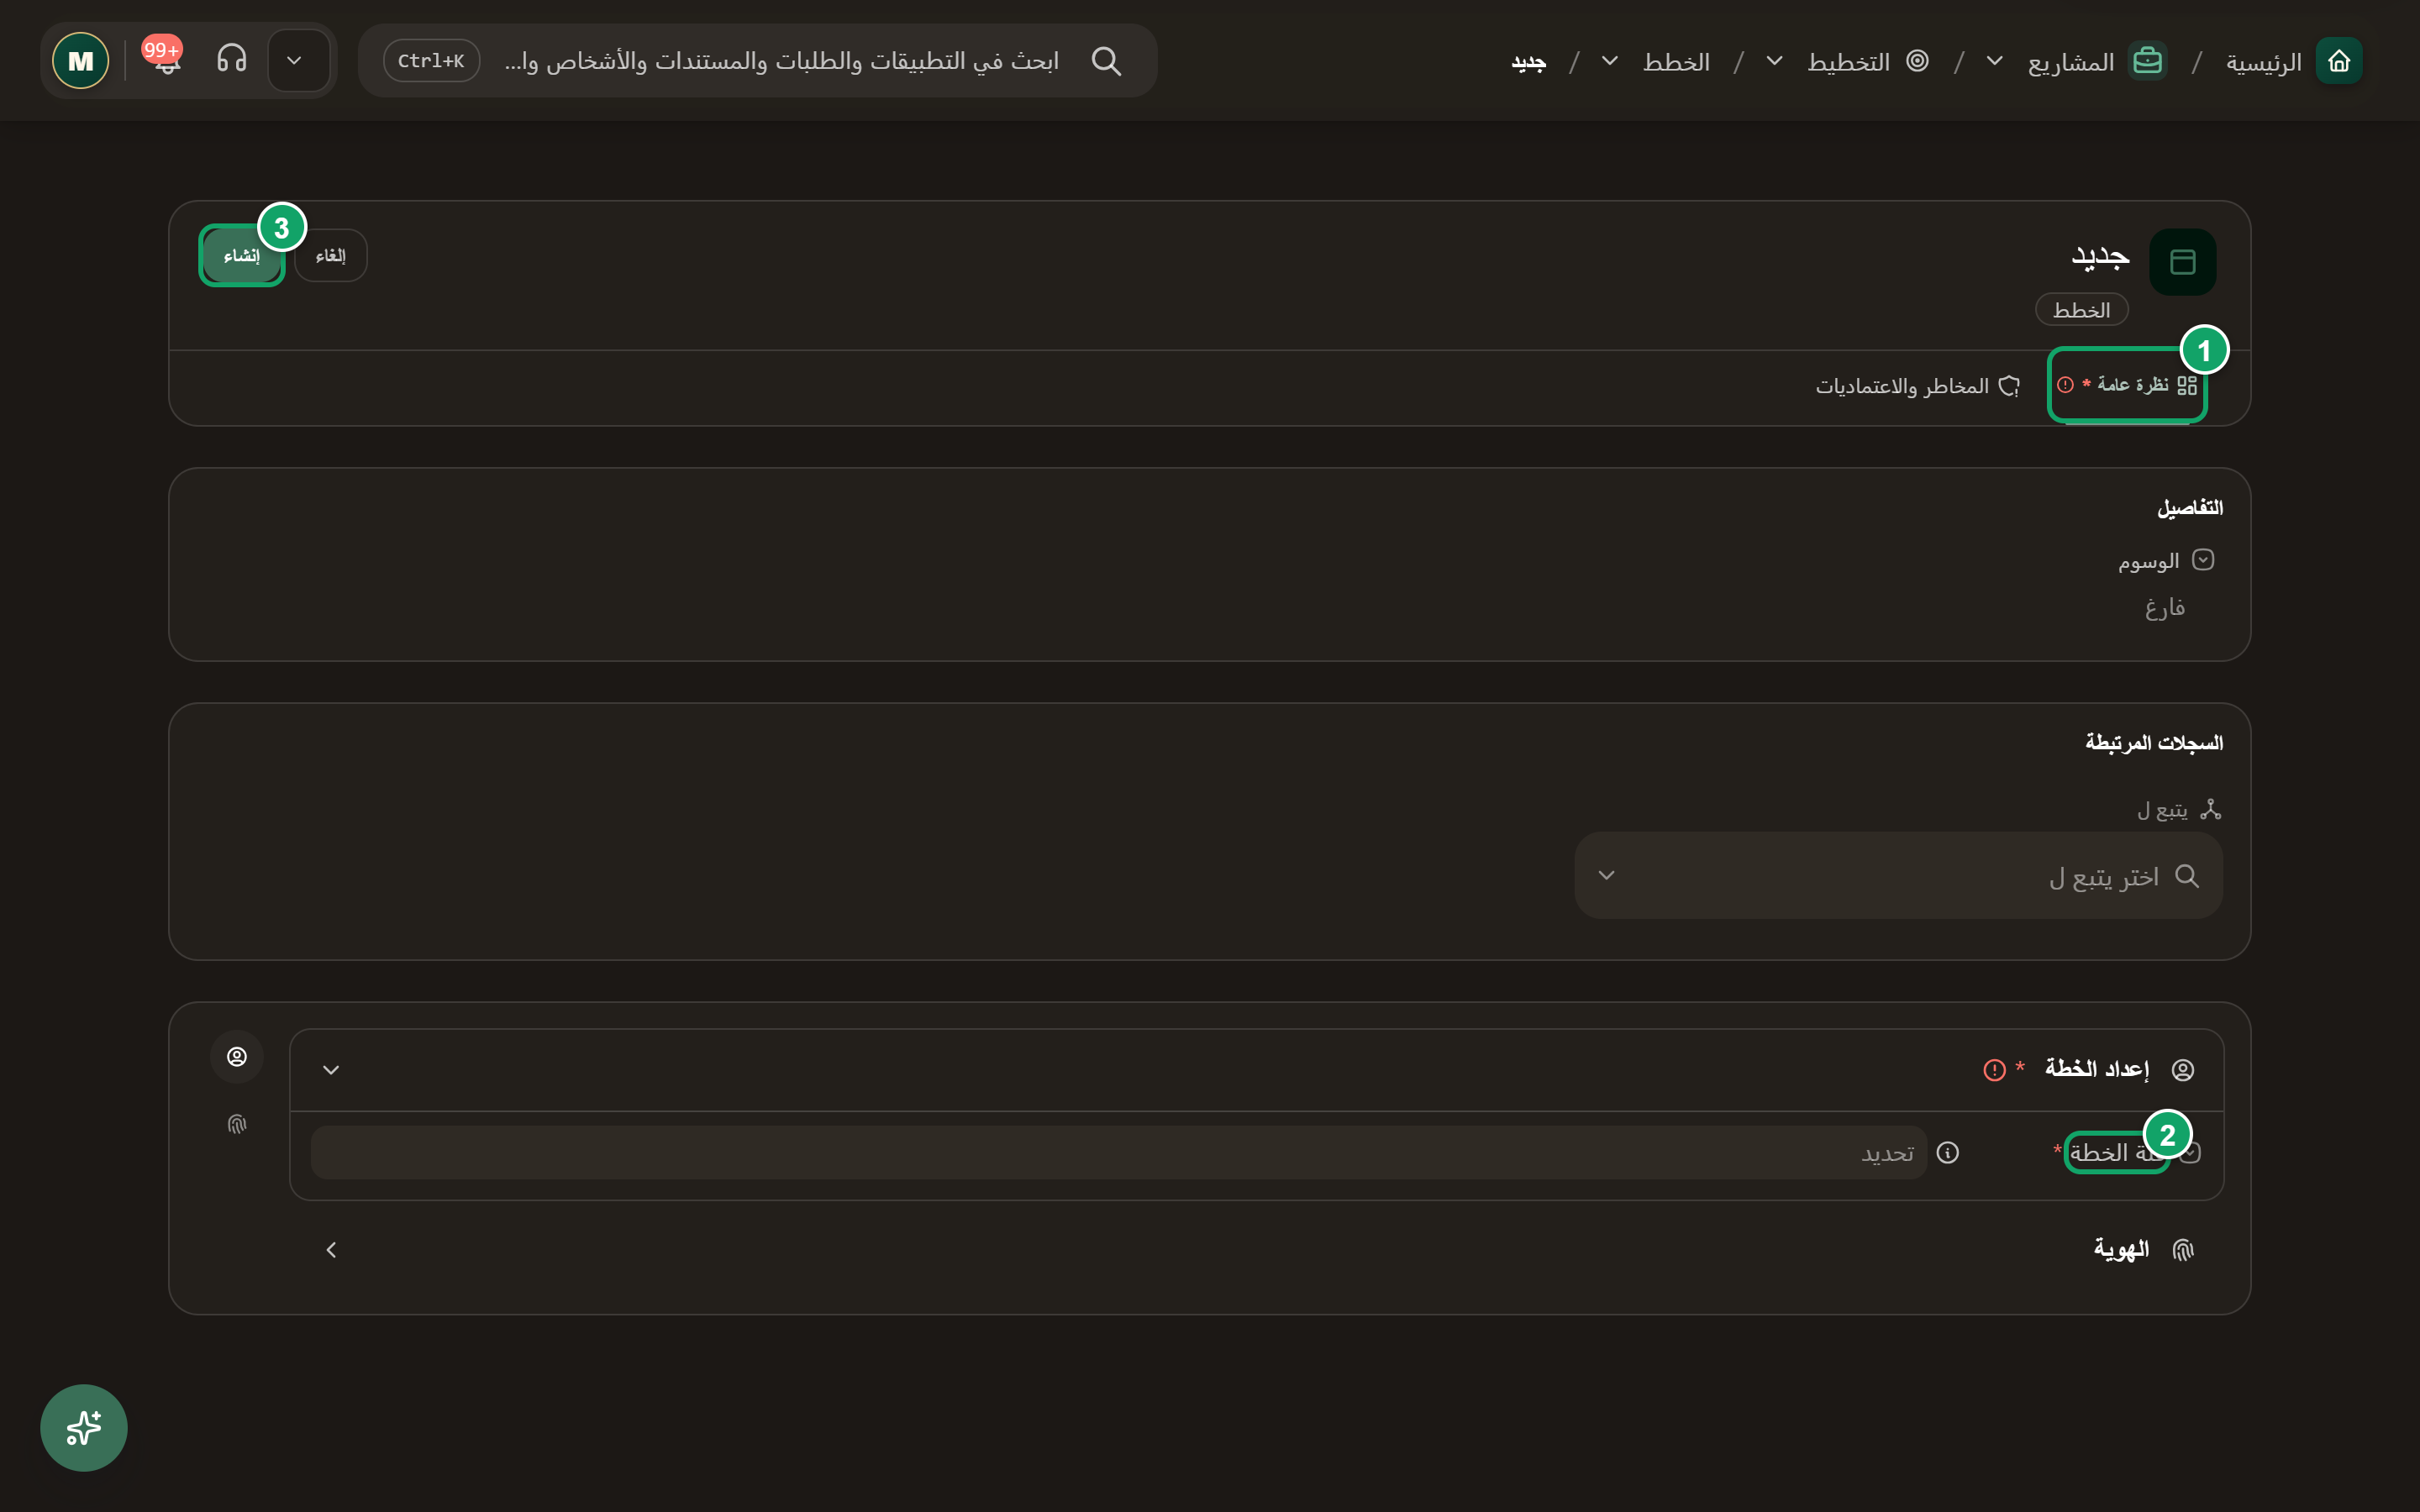
\includegraphics[width=0.95\linewidth,height=0.72\textheight,keepaspectratio]{figures/screens/ch05-plans-ar.png}
\caption{بداية إنشاء خطة قبل اختيار فئتها}
\label{fig:projects-screen-plans}
\shotnote{يبدأ النموذج بحقل «فئة الخطة»، ثم تظهر الاختيارات المناسبة للفئة. لذلك لا تتوقع رؤية جميع بيانات الخطة أو تبويباتها قبل تحديد ما تريد التخطيط له؛ الصورة تعرض نموذجاً غير محفوظ. ① تبويب «نظرة عامة» الذي تبدأ منه الخطة. ② «فئة الخطة»: الحقل الإلزامي الأول، وتظهر بقية الحقول بحسبه. ③ «إنشاء»: يحفظ الخطة بعد إكمال الحقول الإلزامية.}
\end{figure}
\begin{table}[H]
\centering
\caption{ما الذي تسجّله؟}
\label{tab:projects-plans-fields}
\begin{tabularx}{\linewidth}{R{4.2cm} Y}
\rcHeaderRow
\thh{نوع البيانات} & \thh{الحقول}\\
بيانات إلزامية & «فئة الخطة».\\
بيانات إلزامية عند ظهورها & «نوع الخطة»، «الجهة المستهدفة الرئيسية»، «الإطار الأساسي»، «الاسم»، «الأولوية»، «تاريخ البدء»، «تاريخ الانتهاء»، «المالك المسؤول»، «ملف مصدر الإجراء»، «نوع القيد المالي»، «قيمة الغلاف المالي»، «عملة الغلاف المالي»، «رابط الميزانية الإلزامي»، «التفويض»، «منطق الخدمة / عبء العمل»، «منهج تخطيط عبء العمل»، «تاريخ السريان»، «الاختصاص / التغطية»، «نوع السياسة»، «مستوى الإلزام». يعتمد ظهورها على نوع السجل وإعداداته.\\
بيانات إضافية & «الأطر الإضافية»، «الحالة»، «الوصف»، «الأفق التخطيطي»، «وتيرة المراجعة»، «المطّلع»، «الراعي»، «الجهة الحاكمة»، «الوحدة المسؤولة»، «مسؤول المراجعة»، «عقد التغطية»، «مواقع التغطية»، «دورة الخطة»، «جهات النطاق»، «الخطة المرجعية»، «الهدف المرتبط»، «المبادرة المرتبطة»، «السنة المالية»، «حالة التوقع»، «معايير النجاح»، «تاريخ الانتهاء»، «يحل محل الخطة»، «معايير الفاعلية»، «ملاحظات التخطيط»، «الوسوم».\\
نتائج يحسبها النظام & «فئة الجهة المستهدفة»، «حالة الصحة»، «ملخص خط الأساس»، «إصدار خط الأساس»، «الإصدار»، «حالة المراجعة»، «يتطلب اعتماداً»، «مرحلة الاعتماد»، «حالة الاعتماد»، «آخر مراجعة في»، «المراجعة القادمة في»، «إشارة إعادة خط الأساس»، «سبب إعادة خط الأساس»، «الجهد المخطط للموارد (ساعات)»، «الجهد الفعلي للموارد (ساعات)»، «ملخص التكلفة المخططة للموارد»، «السعة المخططة للموارد (ساعات)»، «التكلفة المخططة للموارد»، «التكلفة الملتزم بها للموارد»، «ملخص التكلفة الفعلية للموارد»، «التكلفة الفعلية للموارد»، «انحراف تكلفة الموارد»، «ملخص كميات الموارد»، «الكمية المخططة للموارد»، «الكمية الفعلية للموارد»، «نسبة استخدام سعة الموارد \%»، «عدد المخاطر المفتوحة»، «عدد الاعتماديات المعطلة»، «نسبة تغطية المعالجات»، «إجمالي التعرض الكامن»، «إجمالي التعرض المتبقي»، «نسبة تغطية السيناريوهات»، «نسبة اكتمال تحليل الأثر»، «نسبة جاهزية الإجراءات»، «نسبة نجاح التمارين»، «نسبة تغطية الضوابط»، «عدد الملاحظات المفتوحة»، «عدد الحوادث النشطة»، «نسبة التقدم»، «مرحلة حالة الخطة»، «مفتاح ملف الخطة»، «قالب حالة الخطة». راجع بياناتها المصدرية عند اختلاف النتيجة المتوقعة.\\
\end{tabularx}
\end{table}
\begin{table}[H]
\centering
\caption{التبويبات والسجلات المرتبطة}
\label{tab:projects-plans-tabs}
\begin{tabularx}{\linewidth}{R{4.2cm} Y}
\rcHeaderRow
\thh{التبويب} & \thh{ما الذي تجده فيه؟}\\
«نظرة عامة» & «إعداد الخطة»؛ «الهوية»؛ «الملكية والمساءلة»؛ «الحوكمة»؛ «الجدول الزمني»؛ «الغلاف المالي»؛ «التفويض وحجم العمل»\\
«المصدر» & «مصدر الإجراء والمواءمة»\\
«المعالم» & يعرض المعلومات المرتبطة بهذا الجانب عندما تنطبق إعدادات السجل.\\
«التنفيذ» & «سجل التنفيذ»؛ «حزم العمل»؛ «مسارات حزم العمل»؛ «المخرجات»؛ «نموذج المعالم»؛ «سجل المعالم»؛ «المشكلات والعوائق»؛ «التصعيدات»؛ «التزامات الخدمة»؛ «قياسات الخدمة»؛ «إخلالات الخدمة»؛ «إجراءات الاستعادة»؛ «طلبات التغيير»؛ «مراجعات البوابة»؛ معالم التخطيط (\ref{sec:projects-feature-planning-milestones})؛ هيكل العمل / حزم العمل (\ref{sec:projects-feature-wbs-items})؛ المخرجات / المنتجات (\ref{sec:projects-feature-deliverables})\\
«المواءمة» & «روابط الهرمية والمواءمة»\\
«التغطية» & «التغطية»\\
«النطاق» & «الجهة المستهدفة الأساسية»؛ «النطاق الإضافي»\\
«الإطار» & «نموذج الإطار»؛ «المحاور الاستراتيجية»؛ «الأهداف»؛ «مقاييس بطاقة الأداء»؛ «خريطة الاستراتيجية»؛ «دورات OKR»؛ «النتائج الرئيسية»؛ «مسارات المراجعات»؛ «مواءمة هوشين»؛ «مصفوفة X / كاتشبول»؛ «النماذج المنطقية»؛ «عناصر مسار التغيير»؛ «سلسلة النتائج»؛ «السياق / الجهات / المسار السببي»؛ «دورة حياة السياسة»؛ «تدابير السياسة»؛ «نموذج خارطة الطريق»؛ «عناصر خارطة الطريق»؛ «مسارات الأهداف»؛ المحاور التخطيطية (\ref{sec:projects-feature-planning-themes})؛ أهداف التخطيط (\ref{sec:projects-feature-planning-objectives})؛ دورات OKR (\ref{sec:projects-feature-planning-okrs})؛ النتائج الرئيسية (\ref{sec:projects-feature-planning-key-results})؛ متابعات النتائج الرئيسية (\ref{sec:projects-feature-planning-key-result-checkins})؛ عناصر هوشين (\ref{sec:projects-feature-planning-hoshin-items})؛ روابط مصفوفة X لهوشين (\ref{sec:projects-feature-planning-hoshin-x-matrix-links})؛ تبادلات كاتشبّول لهوشين (\ref{sec:projects-feature-planning-hoshin-catchball-exchanges})؛ الإجراءات المضادة لهوشين (\ref{sec:projects-feature-planning-hoshin-countermeasures})؛ نظرية التغيير (\ref{sec:projects-feature-theory-of-change})؛ أطر النتائج (\ref{sec:projects-feature-logframes})؛ أهداف الإطار المنطقي (\ref{sec:projects-feature-logframe-goals})؛ نتائج الإطار المنطقي (\ref{sec:projects-feature-logframe-outcomes})؛ مخرجات الإطار المنطقي (\ref{sec:projects-feature-logframe-outputs})؛ أنشطة الإطار المنطقي (\ref{sec:projects-feature-logframe-activities})\\
«المبادرات» & «المبادرات الأصلية»؛ المبادرات التخطيطية (\ref{sec:projects-feature-planning-initiatives})\\
«المخرجات» & يعرض المعلومات المرتبطة بهذا الجانب عندما تنطبق إعدادات السجل.\\
«الحوكمة» & «اعتمادات دورة الحياة»؛ «جدولة المراجعة»؛ «المراجعات الحوكمية»؛ «القرارات»؛ «سجل التغييرات»؛ «الإصدارات وخطوط الأساس»؛ مراجعات التخطيط (\ref{sec:projects-feature-planning-reviews})؛ اعتمادات التخطيط (\ref{sec:projects-feature-planning-approvals})؛ قرارات التخطيط (\ref{sec:projects-feature-planning-decisions})\\
«الميزانية» & «نموذج الميزانية»؛ «الميزانيات»؛ «بنود الميزانية»؛ «فترات الميزانية»؛ الميزانيات (\ref{sec:projects-feature-budgets})؛ بنود الميزانية (\ref{sec:projects-feature-budget-lines})؛ فترات بند الميزانية (\ref{sec:projects-feature-budget-line-periods})\\
«التمويل» & «نموذج التمويل»؛ «مصادر التمويل»؛ مصادر التمويل (\ref{sec:projects-feature-funding-sources})\\
«القوى العاملة» & «نموذج القوى العاملة»؛ «احتياجات التوظيف»؛ «المناصب»؛ «التعيينات»\\
«التوظيف» & «نموذج التوظيف»؛ «الشواغر»\\
«المشتريات» & «نموذج المشتريات»؛ «المشتريات»؛ المشتريات (\ref{sec:projects-feature-procurements})\\
«العقود» & «نموذج العقود»\\
«الطلب والسعة» & «نموذج الطلب والسعة»\\
«التخصيصات» & «نموذج التخصيص»؛ «تخصيصات السعة»\\
«المسار» & «مسار جمع التمويل»؛ «الفرص»\\
«المنح والالتزامات» & «المنح والقيود»\\
«الأصول» & «نموذج سجل الأصول»؛ «سجل الأصول»\\
«دورة الحياة» & «نموذج دورة الحياة»؛ «أحداث دورة الحياة»\\
«البوابات» & يعرض المعلومات المرتبطة بهذا الجانب عندما تنطبق إعدادات السجل.\\
«التصعيدات» & يعرض المعلومات المرتبطة بهذا الجانب عندما تنطبق إعدادات السجل.\\
«ضبط التغيير» & يعرض المعلومات المرتبطة بهذا الجانب عندما تنطبق إعدادات السجل.\\
«الموارد» & «نموذج الموارد»؛ «سجل الموارد»؛ موارد التخطيط (\ref{sec:projects-feature-planning-resources})؛ تخصيص الموارد (\ref{sec:projects-feature-resource-allocations})\\
«المخاطر والاعتماديات» & «نموذج المخاطر»؛ «المخاطر»؛ «الاعتماديات»؛ اعتماديات التخطيط (\ref{sec:projects-feature-planning-dependencies})؛ سجل المخاطر (\ref{sec:projects-feature-planning-risks})\\
«الأداء» & «نموذج الأداء»؛ «الأهداف المرحلية»؛ «المؤشرات»؛ «قياسات المؤشرات»؛ «مسارات القياسات»؛ مؤشرات الأداء (\ref{sec:projects-feature-performance-indicators})؛ الأهداف المرحلية (\ref{sec:projects-feature-planning-time-targets})\\
«البيانات» & «مصادر البيانات»؛ «بروتوكولات المؤشرات»؛ «فترات التقارير»؛ «مراجعات جودة البيانات»؛ «سجل الأدلة»؛ فترات التقارير (\ref{sec:projects-feature-planning-reporting-periods})؛ مصادر بيانات التخطيط (\ref{sec:projects-feature-planning-data-sources})؛ عناصر الأدلة (\ref{sec:projects-feature-planning-evidence-items})\\
«التقييم» & «أسئلة التقييم»؛ «نتائج التقييم»؛ «استجابات الإدارة»؛ أسئلة التقييم (\ref{sec:projects-feature-planning-evaluation-questions})؛ نتائج التقييم (\ref{sec:projects-feature-planning-evaluation-findings})؛ استجابات الإدارة (\ref{sec:projects-feature-planning-management-responses})\\
«التعلم» & «أجندة التعلم»؛ «رؤى التعلم»؛ بنود أجندة التعلم (\ref{sec:projects-feature-planning-learning-agenda-items})؛ رؤى التعلم (\ref{sec:projects-feature-planning-learning-insights})\\
«التحسين» & «فرص التحسين»؛ فرص التحسين (\ref{sec:projects-feature-planning-improvement-opportunities})\\
«الافتراضات» & «الافتراضات»؛ «سجل الافتراضات»؛ افتراضات التخطيط (\ref{sec:projects-feature-planning-assumptions})\\
«الدورة» & «نموذج الدورة»\\
«المشاورات» & «سجل المشاورات»\\
«النشر» & «الإصدارات»\\
«الالتزامات» & يعرض المعلومات المرتبطة بهذا الجانب عندما تنطبق إعدادات السجل.\\
«القياسات» & يعرض المعلومات المرتبطة بهذا الجانب عندما تنطبق إعدادات السجل.\\
«الإخلالات» & يعرض المعلومات المرتبطة بهذا الجانب عندما تنطبق إعدادات السجل.\\
«الاستعادة» & «أهداف التعافي»؛ «نطاق التعافي»؛ «تسلسل الاستعادة والتحويل»\\
«الضوابط» & «نموذج الضوابط»؛ «سجل الضوابط»؛ ضوابط التخطيط (\ref{sec:projects-feature-planning-controls})\\
«التقييمات» & «تقييمات الضوابط»؛ تقييمات الضوابط (\ref{sec:projects-feature-planning-control-assessments})\\
«الملاحظات» & «سجل الملاحظات»؛ «الإقرارات واعتمادات الإغلاق»؛ ملاحظات التخطيط (\ref{sec:projects-feature-planning-findings})\\
«الحوادث» & «سجل الحوادث»؛ «الخطورة والتصنيف»؛ حوادث التخطيط (\ref{sec:projects-feature-planning-incidents})\\
«الخط الزمني» & «الخط الزمني للحادث»؛ أحداث الخط الزمني للحوادث (\ref{sec:projects-feature-planning-incident-events})\\
«ما بعد الحادث» & «مراجعة ما بعد الحادث»\\
«السيناريوهات» & «سجل السيناريوهات»؛ «مصفوفة المحفزات»؛ «معايير التفعيل»؛ سيناريوهات التخطيط (\ref{sec:projects-feature-planning-scenarios})\\
«الكتب التشغيلية» & «نموذج الكتب التشغيلية»\\
«تحليل أثر الأعمال» & «نموذج تحليل الأثر»؛ «سجل تحليل الأثر»؛ سجلات تحليل أثر الأعمال (\ref{sec:projects-feature-planning-bia-entries})\\
«الاستمرارية» & «استراتيجيات الاستمرارية»؛ «الحلول اليدوية البديلة»\\
«الإجراءات» & «الإجراءات والكتب التشغيلية»؛ إجراءات التخطيط (\ref{sec:projects-feature-planning-procedures})\\
«التمارين» & «التمارين والاختبارات»؛ تمارين التخطيط (\ref{sec:projects-feature-planning-exercises})\\
«الاختبارات» & «برنامج اختبارات التعافي»\\
\end{tabularx}
\end{table}
\begin{figure}[H]
\centering
\begin{tikzpicture}[node distance=0.5cm]
\node[stepBox] (n0) {\RL{اختيار صفحة العمل}};
\node[stepBox,below=of n0] (n1) {\RL{الخطط}};
\node[stepBox,below=of n1] (n2) {\RL{الحفظ ثم إعادة الفتح}};
\draw[flowsTo] (n0) -- (n1);
\draw[flowsTo] (n1) -- (n2);
\end{tikzpicture}
\rclegend
\caption{مسار العمل والتحقق}
\label{fig:projects-plans-flow}
\shotnote{يبدأ العمل بفتح «الخطط» واختيار السجل الصحيح قبل إدخال التفاصيل. إعادة فتحه بعد الحفظ تؤكد بقاء البيانات، لكنها لا تعني اعتمادها أو اكتمال العمل المرتبط بها.}
\end{figure}

\subsection{خطوات العمل والتحقق}
\begin{enumerate}
\item افتح «الخطط» من تطبيق «المشاريع»، ثم اضغط «إضافة». اختر «فئة الخطة» أولاً، ثم النوع المتاح الذي يطابق العمل المطلوب.
\item اختر «الجهة المستهدفة الرئيسية» من السجلات المتاحة، ثم «الإطار الأساسي». أكمل الاسم والمالك المسؤول والأولوية وتاريخي البدء والانتهاء، ثم راجع أي حقول إضافية يطلبها النوع المختار.
\item اضغط «إنشاء»، ثم أعد فتح الخطة. تحقق من الجهة والمالك والفترة، وافتح الأقسام المتاحة لإضافة الأهداف أو التنفيذ أو القياس حسب نوعها.
\item راجع مرحلة الخطة قبل تعديلها؛ فقد لا تسمح المرحلة الحالية بتغيير الإعدادات أو إضافة بعض السجلات. عالج رسالة التحقق أو اطلب مراجعة الصلاحية بدلاً من تكرار الخطة.
\end{enumerate}

\textbf{تطبيق المثال:} في المثال الافتراضي، استخدم «خطة تحسين جاهزية فرع حلب» في «الاسم»، ثم أكمل بقية البيانات بما يناسب عمل الأفق. لا تستخدم قيم المثال بديلاً عن السجلات الفعلية المطلوبة في حقول الربط.

\textbf{تحقق ومعالجة المشكلة:} يجب أن تجد السجل بعد إعادة فتحه وأن تبقى البيانات التي حفظتها. إذا لم يظهر، فراجع البحث والفلاتر والنطاق وصلاحية الوصول قبل إنشائه مرة أخرى. وإذا تعذر الحفظ، فأكمل الحقول المطلوبة ورسائل التحقق؛ أما غياب تبويب أو قفل حقل فيستدعي مراجعة نوع السجل وإطاره ومرحلته مع المسؤول.

\clearpage
\section{المشاريع}
\label{sec:projects-feature-projects}

يجمع المشروع عملاً محدد النطاق له مدير ونتيجة مطلوبة. ابدأ بتعريفه وميثاقه، ثم استخدم الأقسام المتاحة لتخطيط التنفيذ ومراجعة التقدم.

\begin{rcnote}[مثال: شركة الأفق]
تنشئ سارة مشروع «تجهيز زيارة فرع حلب» بالرمز \en{HZN-PRJ-01}، وتحدّد النتيجة المطلوبة في الميثاق. يتولى عمر إعداد ملف الزيارة بعد تحديد مسؤوليته، وتراجع سارة المخرج عند التسليم.
\end{rcnote}

\textbf{المسار ومن يستخدمه:} افتح تطبيق «المشاريع»، ثم بطاقة «المشاريع». هذه صفحة رئيسية في التطبيق. يستخدمها المسؤول عن هذا العمل، ويعدّل الموظف البيانات المسموح له بها وفق صلاحياته.

\subsection{الميثاق يسبق التخطيط التفصيلي}
يجمع تبويب «ميثاق المشروع» الغرض والأهداف ومعايير النجاح والنطاق وما يقع خارجه، ودراسة الجدوى والافتراضات والمخاطر وبيانات الاعتماد. راجع «مدير المشروع» و«الراعي» والتواريخ، ولا تعتبر حفظ السجل اعتماداً للميثاق.

يتطلب ظهور أقسام التخطيط أن تكون «حالة الميثاق» معتمدة وأن يتجاوز المشروع مرحلة الإعداد. ويحدد «الإطار المنهجي» و«نهج التسليم» ما يظهر من مراحل وسباقات وحوكمة، بينما تؤثر طبيعة المشروع والعميل في المشتريات والمتابعة والتقييم. بعد الاعتماد قد تُقفل بيانات الإعداد، ويُراجع تعديلها عبر ضبط التغيير.

\textbf{التقدم والحالة:} تُحسب نسبة التقدم من سجلات التنفيذ ذات الصلة. راجع حزم العمل والمخرجات والمؤشرات قبل تفسير حالة المشروع؛ ولا تخلط اكتمال مهمة منفردة باكتمال المشروع كله.
\begin{figure}[H]
\centering
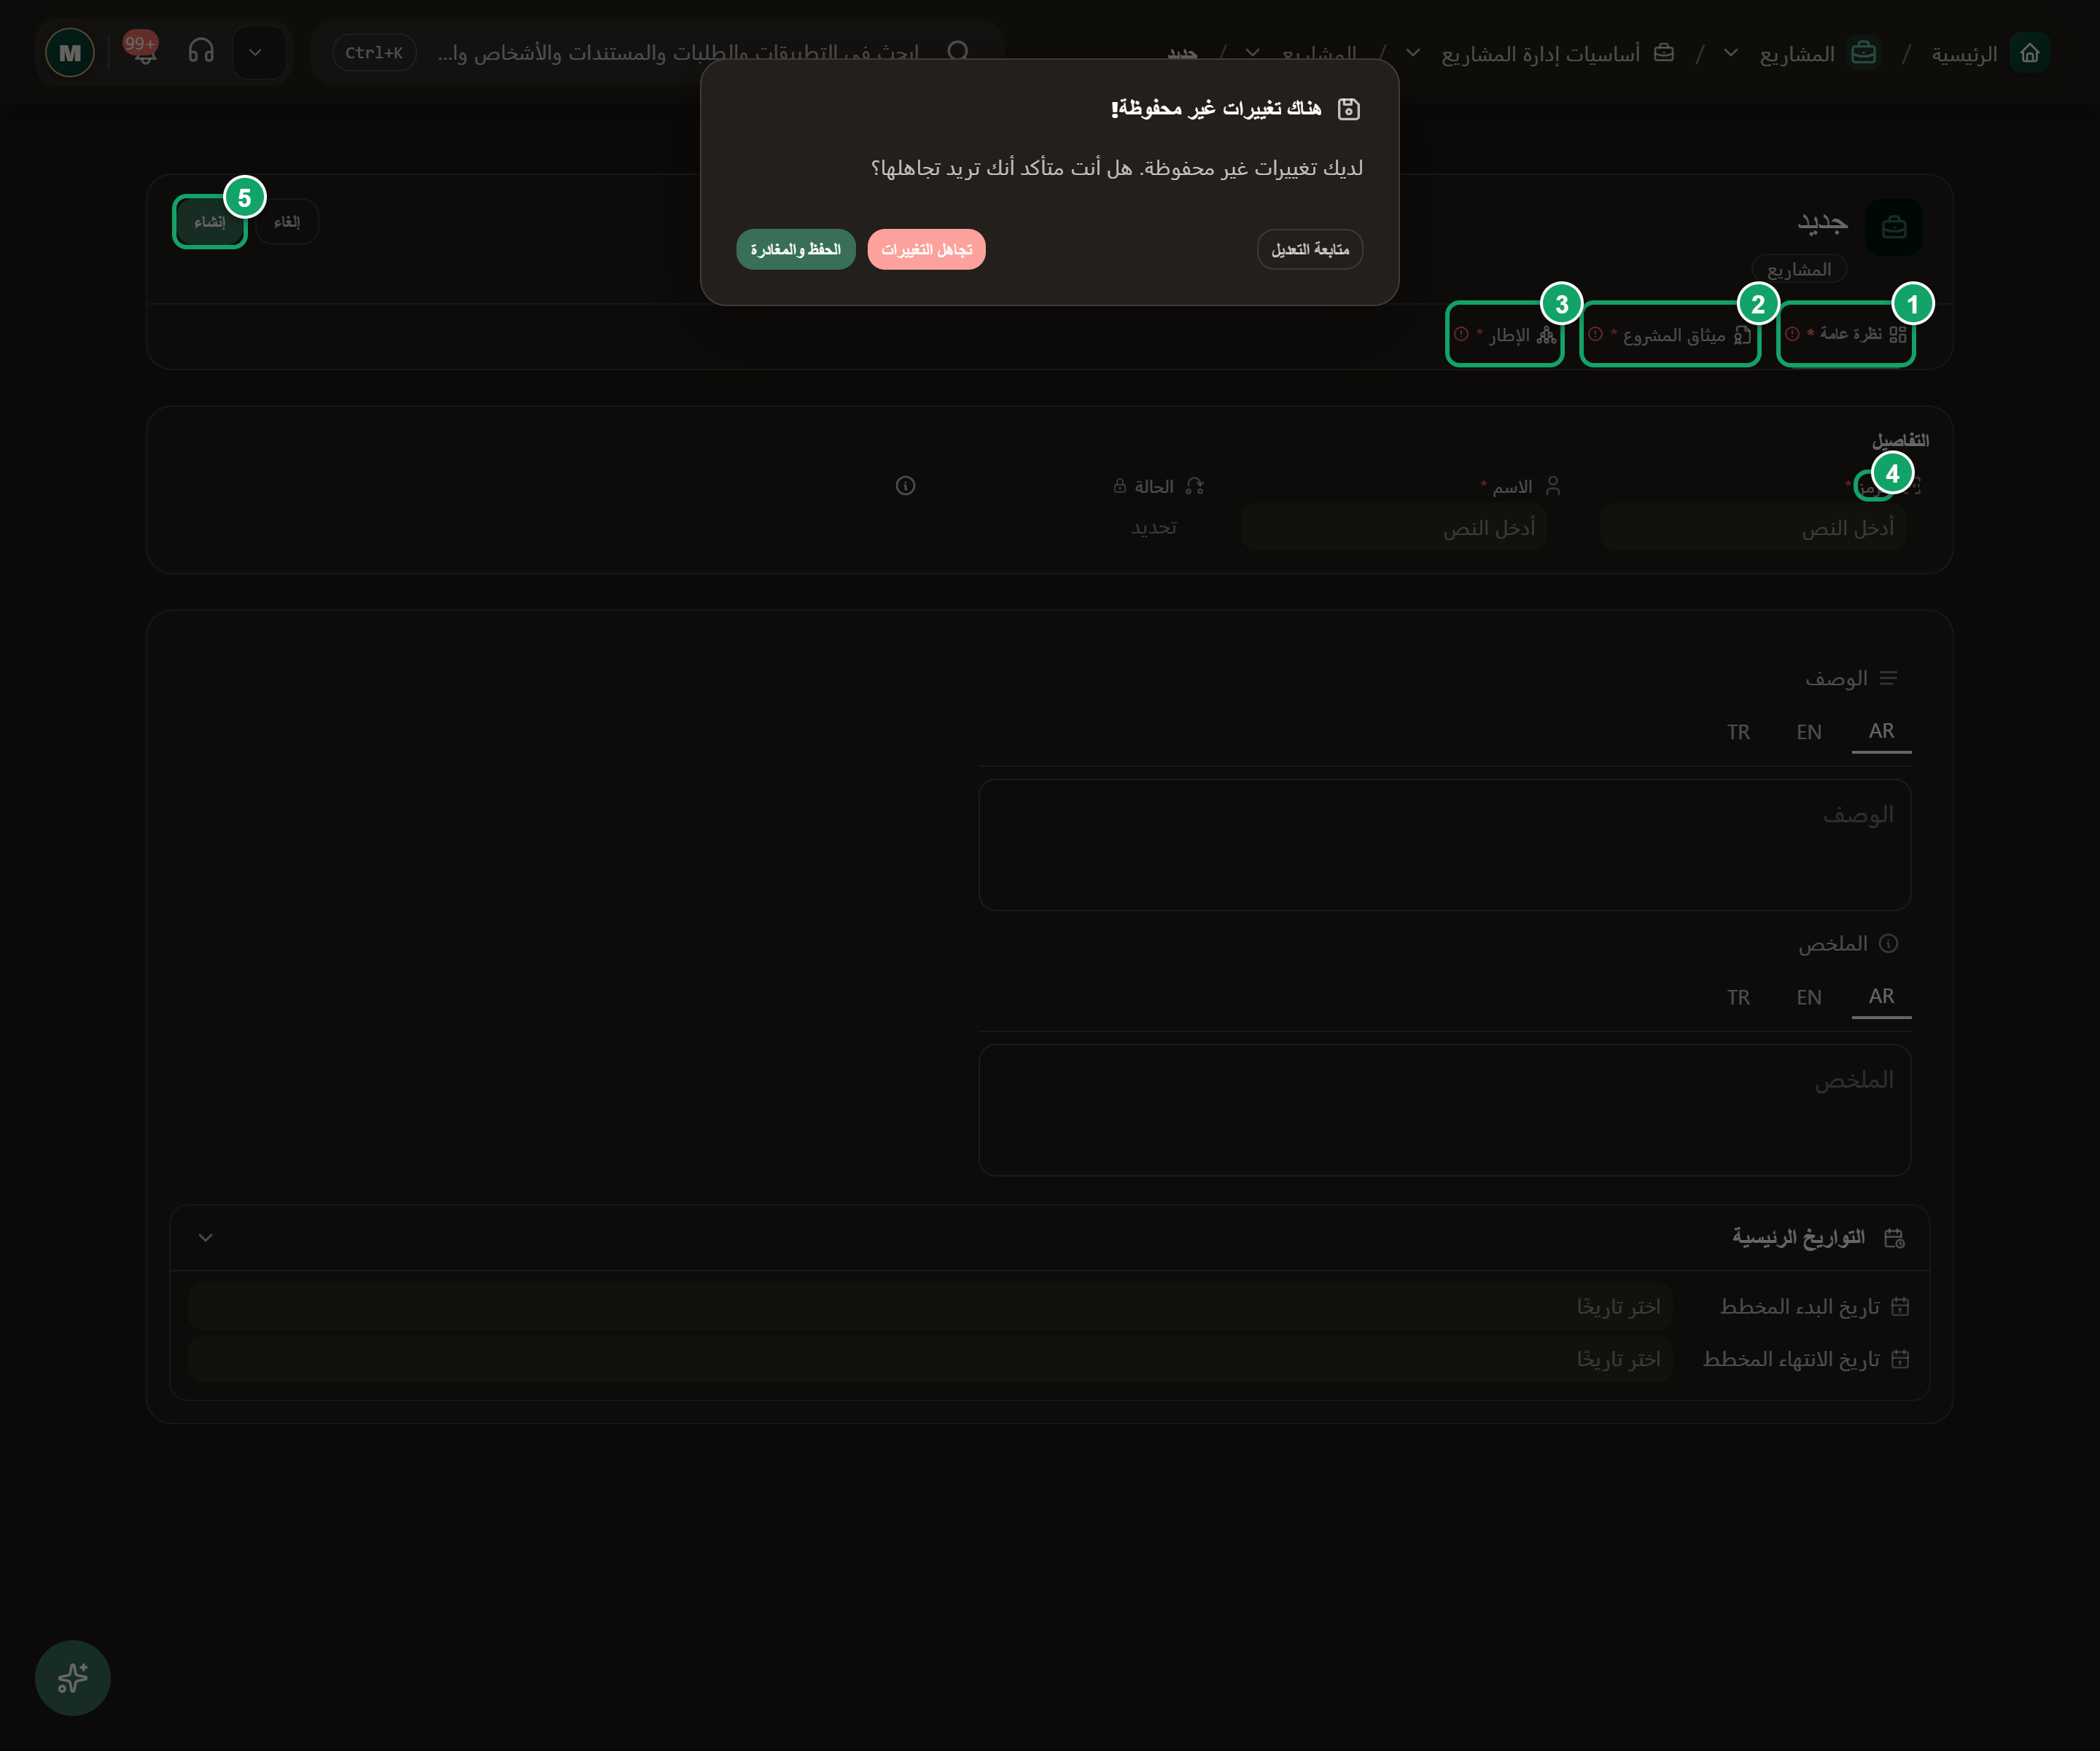
\includegraphics[width=0.95\linewidth,height=0.72\textheight,keepaspectratio]{figures/screens/ch05-project-create-ar.png}
\caption{نظرة عامة على مشروع جديد غير محفوظ}
\label{fig:projects-screen-project-create}
\shotnote{يجمع هذا التبويب هوية المشروع ووصفه وتواريخه المخططة. ظهور الاسم والرمز لا يكفي لإكمال الإنشاء؛ يطلب التبويبان الآخران بيانات الميثاق والإطار، وتبقى حالة المشروع مرتبطة بإعداداته. ① تبويب «نظرة عامة». ② تبويب «ميثاق المشروع». ③ تبويب «الإطار»؛ وتعني العلامة الحمراء أن في التبويب حقلاً إلزامياً فارغاً. ④ «الرمز»: أول الحقول الإلزامية. ⑤ «إنشاء».}
\end{figure}
\begin{figure}[H]
\centering
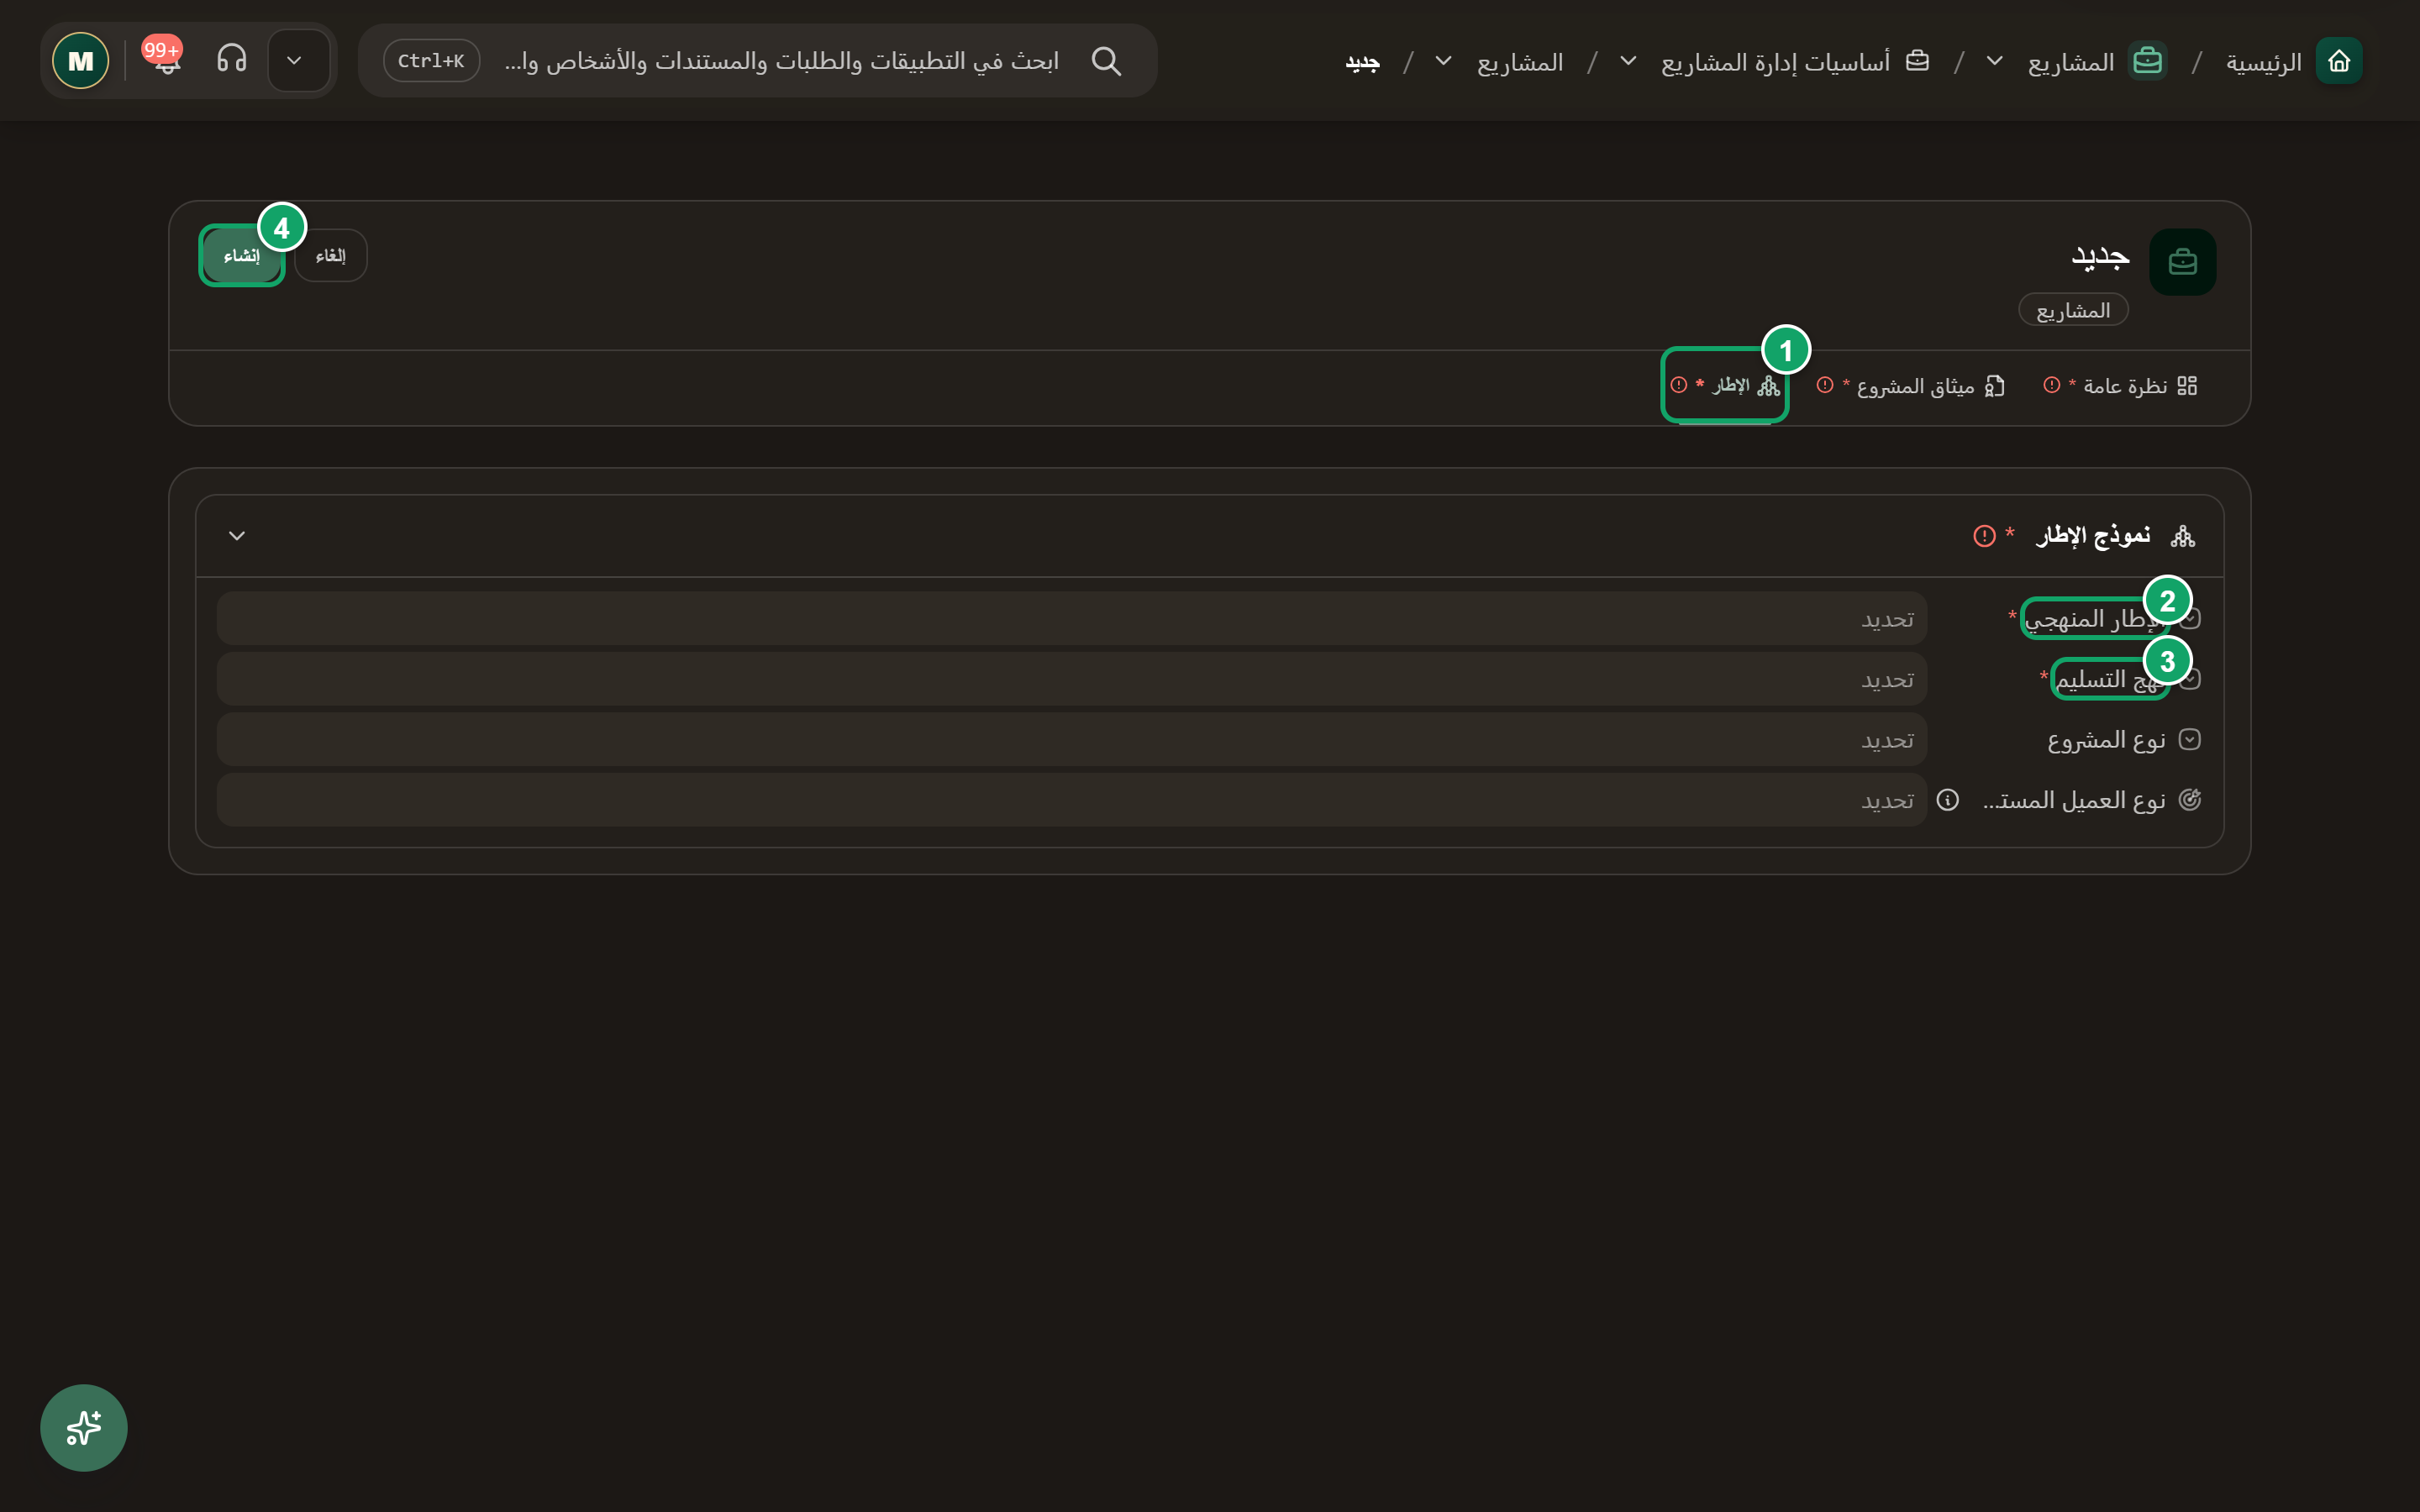
\includegraphics[width=0.95\linewidth,height=0.72\textheight,keepaspectratio]{figures/screens/ch05-project-framework-ar.png}
\caption{اختيار إطار المشروع ونهج التسليم}
\label{fig:projects-screen-project-framework}
\shotnote{يحدد «الإطار المنهجي» و«نهج التسليم» طريقة تنظيم المشروع والأقسام المناسبة له. راجع أيضاً نوع المشروع والعميل المستهدف، لأنهما يساعدان على تحديد الحاجة إلى المشتريات والمتابعة؛ النموذج في الصورة لم يُحفظ. ① تبويب «الإطار». ② «الإطار المنهجي»: الطريقة التي يُدار بها المشروع. ③ «نهج التسليم»: كيف تُسلَّم النتائج. ④ «إنشاء»: يحفظ المشروع بعد إكمال التبويبات الإلزامية.}
\end{figure}
\begin{figure}[H]
\centering
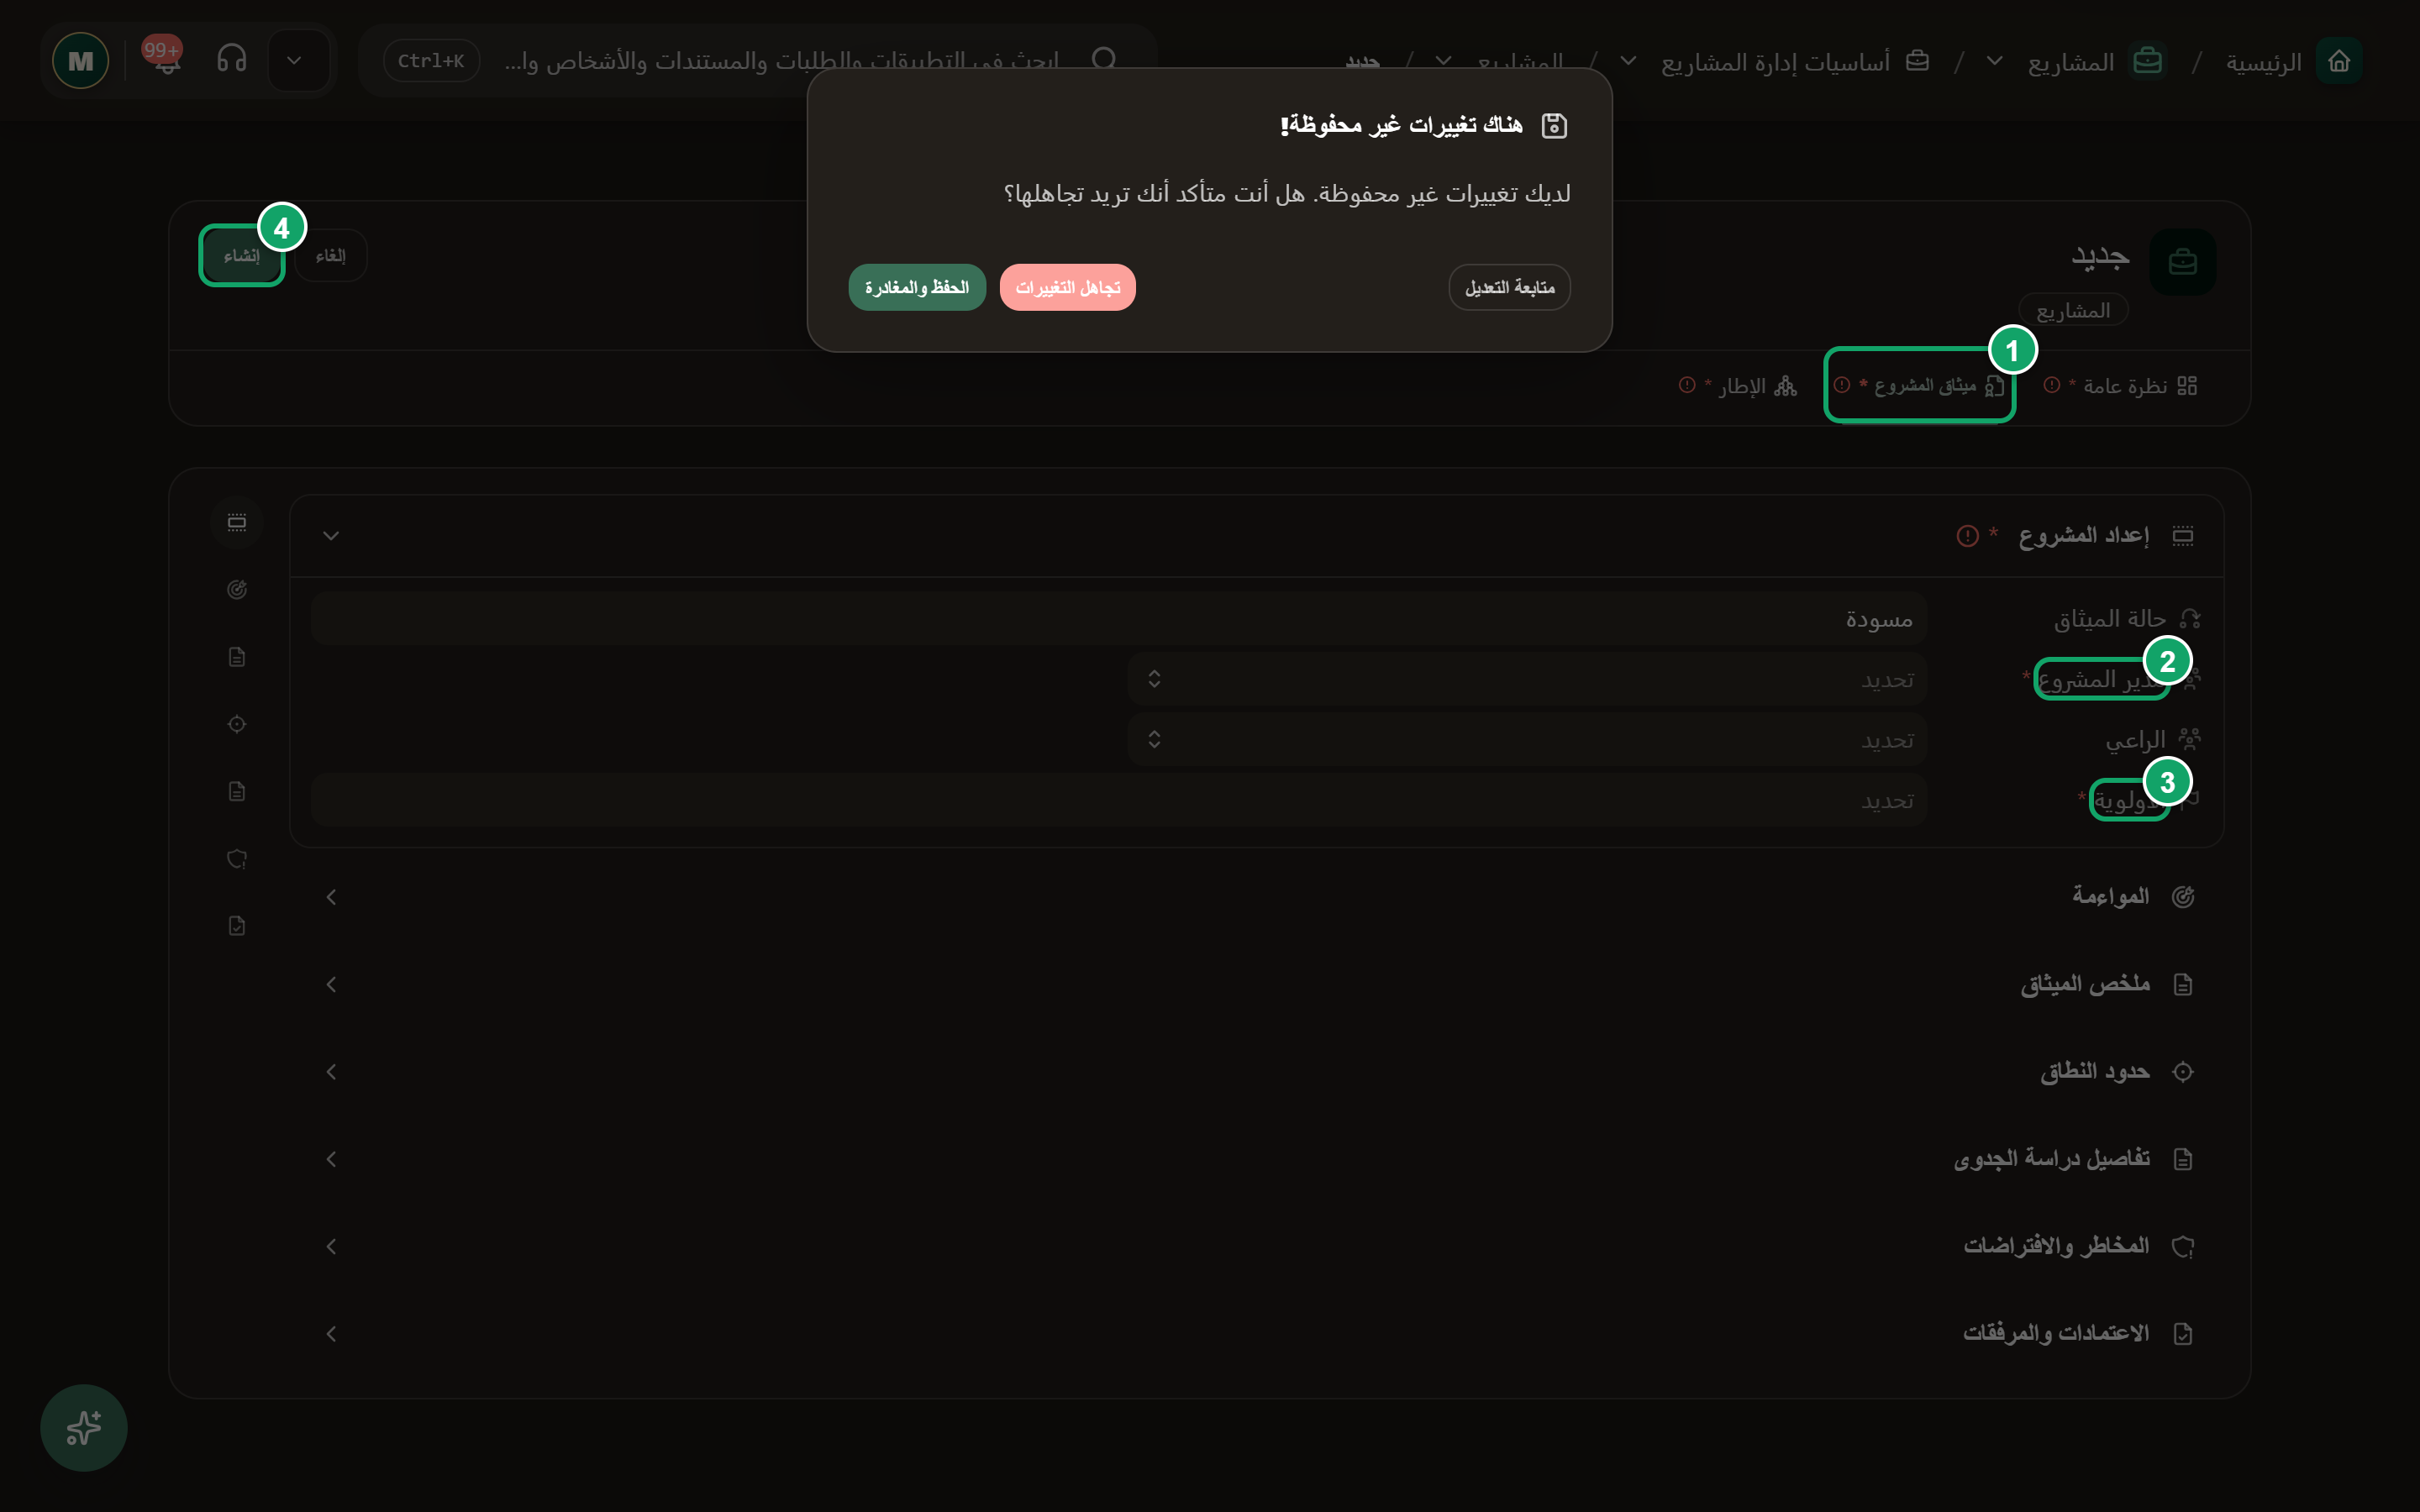
\includegraphics[width=0.95\linewidth,height=0.72\textheight,keepaspectratio]{figures/screens/ch05-project-charter-ar.png}
\caption{إعداد المشروع وأقسام الميثاق}
\label{fig:projects-screen-project-charter}
\shotnote{يظهر الميثاق بحالة «مسودة»، مع اختيار مدير المشروع والراعي والأولوية. تجمع الأقسام الأخرى الغرض والنطاق ودراسة الجدوى والمخاطر والاعتماد؛ فتح التبويب أو حفظ بياناته لا يعني أن الميثاق اعتُمد. ① تبويب «ميثاق المشروع». ② «مدير المشروع». ③ «الأولوية». ④ «إنشاء».}
\end{figure}
\begin{table}[H]
\centering
\caption{ما الذي تسجّله؟}
\label{tab:projects-projects-fields}
\begin{tabularx}{\linewidth}{R{4.2cm} Y}
\rcHeaderRow
\thh{نوع البيانات} & \thh{الحقول}\\
بيانات إلزامية & «الرمز»، «الاسم»، «الإطار المنهجي»، «نهج التسليم»، «مدير المشروع»، «الأولوية».\\
بيانات إضافية & «الوصف»، «نوع المشروع»، «نوع العميل المستهدف»، «الحالة»، «حالة الميثاق»، «عنوان الميثاق»، «الغرض»، «الأهداف»، «معايير النجاح»، «وصف النطاق»، «خارج النطاق»، «نوع دراسة الجدوى»، «التوافق الاستراتيجي»، «الفوائد المتوقعة»، «تأثير أصحاب المصلحة»، «العائد المتوقع»، «الميزانية المقدرة»، «المدة المقدرة (أيام)»، «تاريخ البدء المستهدف»، «تاريخ الانتهاء المستهدف»، «الافتراضات الرئيسية»، «القيود الرئيسية»، «المخاطر الرئيسية»، «اعتمد بواسطة»، «تاريخ الاعتماد»، «المرفقات»، «المحفظة»، «البرنامج»، «الخطط»، «الراعي»، «المالكون»، «المطّلعون»، «تجاوز صحة النطاق»، «تجاوز صحة الجودة»، «تاريخ البدء المخطط»، «تاريخ الانتهاء المخطط»، «تاريخ البدء الفعلي»، «تاريخ الانتهاء الفعلي»، «المرحلة الحالية»، «العملة»، «الميزانية المخططة»، «التكلفة الفعلية»، «القيمة المكتسبة»، «القيمة المخططة»، «القطاع»، «المانحون»، «الإطار المنطقي»، «الوسوم».\\
نتائج يحسبها النظام & «قالب حالة المشروع»، «مرحلة الإعداد»، «ملف الإعداد»، «اكتمل الإعداد»، «الحوكمة مطلوبة»، «الصحة العامة»، «صحة النطاق»، «صحة الجدول الزمني»، «صحة التكلفة»، «صحة الجودة»، «صحة المخاطر»، «مؤشر أداء التكلفة»، «مؤشر أداء الجدول الزمني»، «نسبة التقدم». راجع بياناتها المصدرية عند اختلاف النتيجة المتوقعة.\\
\end{tabularx}
\end{table}
\begin{table}[H]
\centering
\caption{التبويبات والسجلات المرتبطة}
\label{tab:projects-projects-tabs}
\begin{tabularx}{\linewidth}{R{4.2cm} Y}
\rcHeaderRow
\thh{التبويب} & \thh{ما الذي تجده فيه؟}\\
«نظرة عامة» & «الملخص السريع»؛ «التواريخ الرئيسية»\\
«ميثاق المشروع» & «إعداد المشروع»؛ «المواءمة»؛ «ملخص الميثاق»؛ «حدود النطاق»؛ «تفاصيل دراسة الجدوى»؛ «المخاطر والافتراضات»؛ «الاعتمادات والمرفقات»\\
«الإطار» & «نموذج الإطار»؛ المحاور التخطيطية (\ref{sec:projects-feature-planning-themes})؛ أهداف التخطيط (\ref{sec:projects-feature-planning-objectives})؛ دورات OKR (\ref{sec:projects-feature-planning-okrs})؛ النتائج الرئيسية (\ref{sec:projects-feature-planning-key-results})؛ متابعات النتائج الرئيسية (\ref{sec:projects-feature-planning-key-result-checkins})؛ عناصر هوشين (\ref{sec:projects-feature-planning-hoshin-items})؛ روابط مصفوفة X لهوشين (\ref{sec:projects-feature-planning-hoshin-x-matrix-links})؛ تبادلات كاتشبّول لهوشين (\ref{sec:projects-feature-planning-hoshin-catchball-exchanges})؛ الإجراءات المضادة لهوشين (\ref{sec:projects-feature-planning-hoshin-countermeasures})؛ نظرية التغيير (\ref{sec:projects-feature-theory-of-change})؛ أطر النتائج (\ref{sec:projects-feature-logframes})؛ أهداف الإطار المنطقي (\ref{sec:projects-feature-logframe-goals})؛ نتائج الإطار المنطقي (\ref{sec:projects-feature-logframe-outcomes})؛ مخرجات الإطار المنطقي (\ref{sec:projects-feature-logframe-outputs})؛ أنشطة الإطار المنطقي (\ref{sec:projects-feature-logframe-activities})\\
«التنفيذ» & «النطاق / هيكل العمل وحزم العمل»؛ «المخرجات / المنتجات»؛ «ضبط التنفيذ»؛ «المهام / الأنشطة»؛ معالم التخطيط (\ref{sec:projects-feature-planning-milestones})؛ هيكل العمل / حزم العمل (\ref{sec:projects-feature-wbs-items})؛ المخرجات / المنتجات (\ref{sec:projects-feature-deliverables})؛ المتطلبات (\ref{sec:projects-feature-requirements})\\
«الأداء» & «مؤشرات الصحة»؛ «مسارات القياسات»؛ «المؤشرات»؛ «القياسات»؛ «بطاقة الأداء»؛ «جودة البيانات»؛ «تقارير الحالة»؛ «القيمة المكتسبة»؛ تقارير الحالة (\ref{sec:projects-feature-status-reports})؛ مؤشرات الأداء (\ref{sec:projects-feature-performance-indicators})؛ الأهداف المرحلية (\ref{sec:projects-feature-planning-time-targets})\\
«الموارد» & «القيادة»؛ «الملكية والتواصل»؛ «الفريق الأساسي»؛ «أصحاب المصلحة»؛ «مصفوفة المسؤوليات»؛ موارد التخطيط (\ref{sec:projects-feature-planning-resources})؛ أدوار الفريق (\ref{sec:projects-feature-team-roles})؛ مصفوفة المسؤوليات (\ref{sec:projects-feature-raci-entries})؛ تخصيص الموارد (\ref{sec:projects-feature-resource-allocations})؛ أصحاب المصلحة (\ref{sec:projects-feature-stakeholders})\\
«النطاق» & يعرض المعلومات المرتبطة بهذا الجانب عندما تنطبق إعدادات السجل.\\
«الجدول الزمني» & «المرحلة الحالية»؛ مراحل المشروع (\ref{sec:projects-feature-phases})؛ التبعيات (\ref{sec:projects-feature-dependencies})؛ خطوط الأساس (\ref{sec:projects-feature-baselines})\\
«المالية» & «ملخص الميزانية»؛ «تتبع التكاليف»؛ «إدارة القيمة المكتسبة»؛ المصروفات (\ref{sec:projects-feature-expenditures})\\
«الجودة» & معايير الجودة (\ref{sec:projects-feature-quality-criteria})\\
«المخاطر والمشكلات» & اعتماديات التخطيط (\ref{sec:projects-feature-planning-dependencies})؛ سجل المخاطر (\ref{sec:projects-feature-planning-risks})؛ سجل مخاطر إدارة المشاريع (\ref{sec:projects-feature-project-risks})؛ المشكلات (\ref{sec:projects-feature-issues})\\
«الاتصالات» & «خطة الاتصال»؛ خطة الاتصال (\ref{sec:projects-feature-communication-plan})\\
«المشتريات» & المشتريات (\ref{sec:projects-feature-procurements})\\
«الحوكمة» & «البيانات الوصفية»؛ مراجعات التخطيط (\ref{sec:projects-feature-planning-reviews})؛ اعتمادات التخطيط (\ref{sec:projects-feature-planning-approvals})؛ قرارات التخطيط (\ref{sec:projects-feature-planning-decisions})؛ مراجعات البوابة (\ref{sec:projects-feature-gate-reviews})؛ طلبات التغيير (\ref{sec:projects-feature-change-requests})؛ قرارات الاجتماعات (\ref{sec:projects-feature-meeting-decisions})؛ الدروس المستفادة (\ref{sec:projects-feature-lessons-learned})\\
«أجايل» & السباقات (\ref{sec:projects-feature-sprints})؛ تعريف الإنجاز (\ref{sec:projects-feature-definition-of-done})\\
«المتابعة والتقييم» & «إعداد المتابعة والتقييم»؛ المستفيدون (\ref{sec:projects-feature-beneficiaries})\\
\end{tabularx}
\end{table}
\begin{figure}[H]
\centering
\begin{tikzpicture}[node distance=0.5cm]
\node[stepBox] (n0) {\RL{اختيار صفحة العمل}};
\node[stepBox,below=of n0] (n1) {\RL{المشاريع}};
\node[stepBox,below=of n1] (n2) {\RL{الحفظ ثم إعادة الفتح}};
\draw[flowsTo] (n0) -- (n1);
\draw[flowsTo] (n1) -- (n2);
\end{tikzpicture}
\rclegend
\caption{مسار العمل والتحقق}
\label{fig:projects-projects-flow}
\shotnote{يبدأ العمل بفتح «المشاريع» واختيار السجل الصحيح قبل إدخال التفاصيل. إعادة فتحه بعد الحفظ تؤكد بقاء البيانات، لكنها لا تعني اعتمادها أو اكتمال العمل المرتبط بها.}
\end{figure}

\subsection{خطوات العمل والتحقق}
\begin{enumerate}
\item افتح «المشاريع» واضغط «إضافة». في «نظرة عامة»، أدخل الرمز والاسم وحدّد التاريخين المخططين عندما تعرفهما.
\item افتح «الإطار»، واختر «الإطار المنهجي» و«نهج التسليم». راجع نوع المشروع ونوع العميل المستهدف لأنهما يؤثران في الأقسام المتاحة لاحقاً.
\item افتح «ميثاق المشروع»، واختر «مدير المشروع» و«الأولوية». أكمل الغرض والأهداف والنطاق ومعايير النجاح، وراجع الراعي وبيانات الاعتماد مع المسؤول عن المشروع.
\item اضغط «إنشاء» وأعد فتح المشروع. تحقق من اسمه ومديره وإطاره؛ لا تغيّر حالة الميثاق إلى معتمد لمجرد إظهار التبويبات.
\item بعد المراجعة والاعتماد وفق صلاحيات المؤسسة، تحقق من مرحلة الإعداد والتبويبات المتاحة. أضف سجلات التنفيذ المناسبة، ثم راجع التقدم من نتائج العمل الفعلية.
\end{enumerate}

\textbf{تطبيق المثال:} في المثال الافتراضي، استخدم «تجهيز زيارة فرع حلب» في «الاسم»، ثم أكمل بقية البيانات بما يناسب عمل الأفق. لا تستخدم قيم المثال بديلاً عن السجلات الفعلية المطلوبة في حقول الربط.

\textbf{تحقق ومعالجة المشكلة:} يجب أن تجد السجل بعد إعادة فتحه وأن تبقى البيانات التي حفظتها. إذا لم يظهر، فراجع البحث والفلاتر والنطاق وصلاحية الوصول قبل إنشائه مرة أخرى. وإذا تعذر الحفظ، فأكمل الحقول المطلوبة ورسائل التحقق؛ أما غياب تبويب أو قفل حقل فيستدعي مراجعة نوع السجل وإطاره ومرحلته مع المسؤول.

\clearpage
\section{المحافظ}
\label{sec:projects-feature-portfolios}

تجمع المحفظة برامج ومشاريع تخدم توجهاً مشتركاً، وتساعد الإدارة على مراجعة الأولويات والتمويل. أنشئها عندما تحتاج إلى متابعة عدة أعمال معاً؛ فربط المشروع بمحفظة ليس شرطاً عاماً لإنشائه.

\begin{rcnote}[مثال: شركة الأفق]
تجمع إدارة الأفق أعمال تطوير الفروع في محفظة واحدة، وتكلّف سارة بمتابعة المعلومات المتعلقة بزيارة حلب. تراجع الإدارة الأولويات عبر المشاريع المرتبطة دون دمج سجلاتها.
\end{rcnote}

\textbf{المسار ومن يستخدمه:} افتح تطبيق «المشاريع»، ثم بطاقة «المحافظ». هذه صفحة رئيسية في التطبيق. يستخدمها المسؤول عن هذا العمل، ويعدّل الموظف البيانات المسموح له بها وفق صلاحياته.

\begin{figure}[H]
\centering
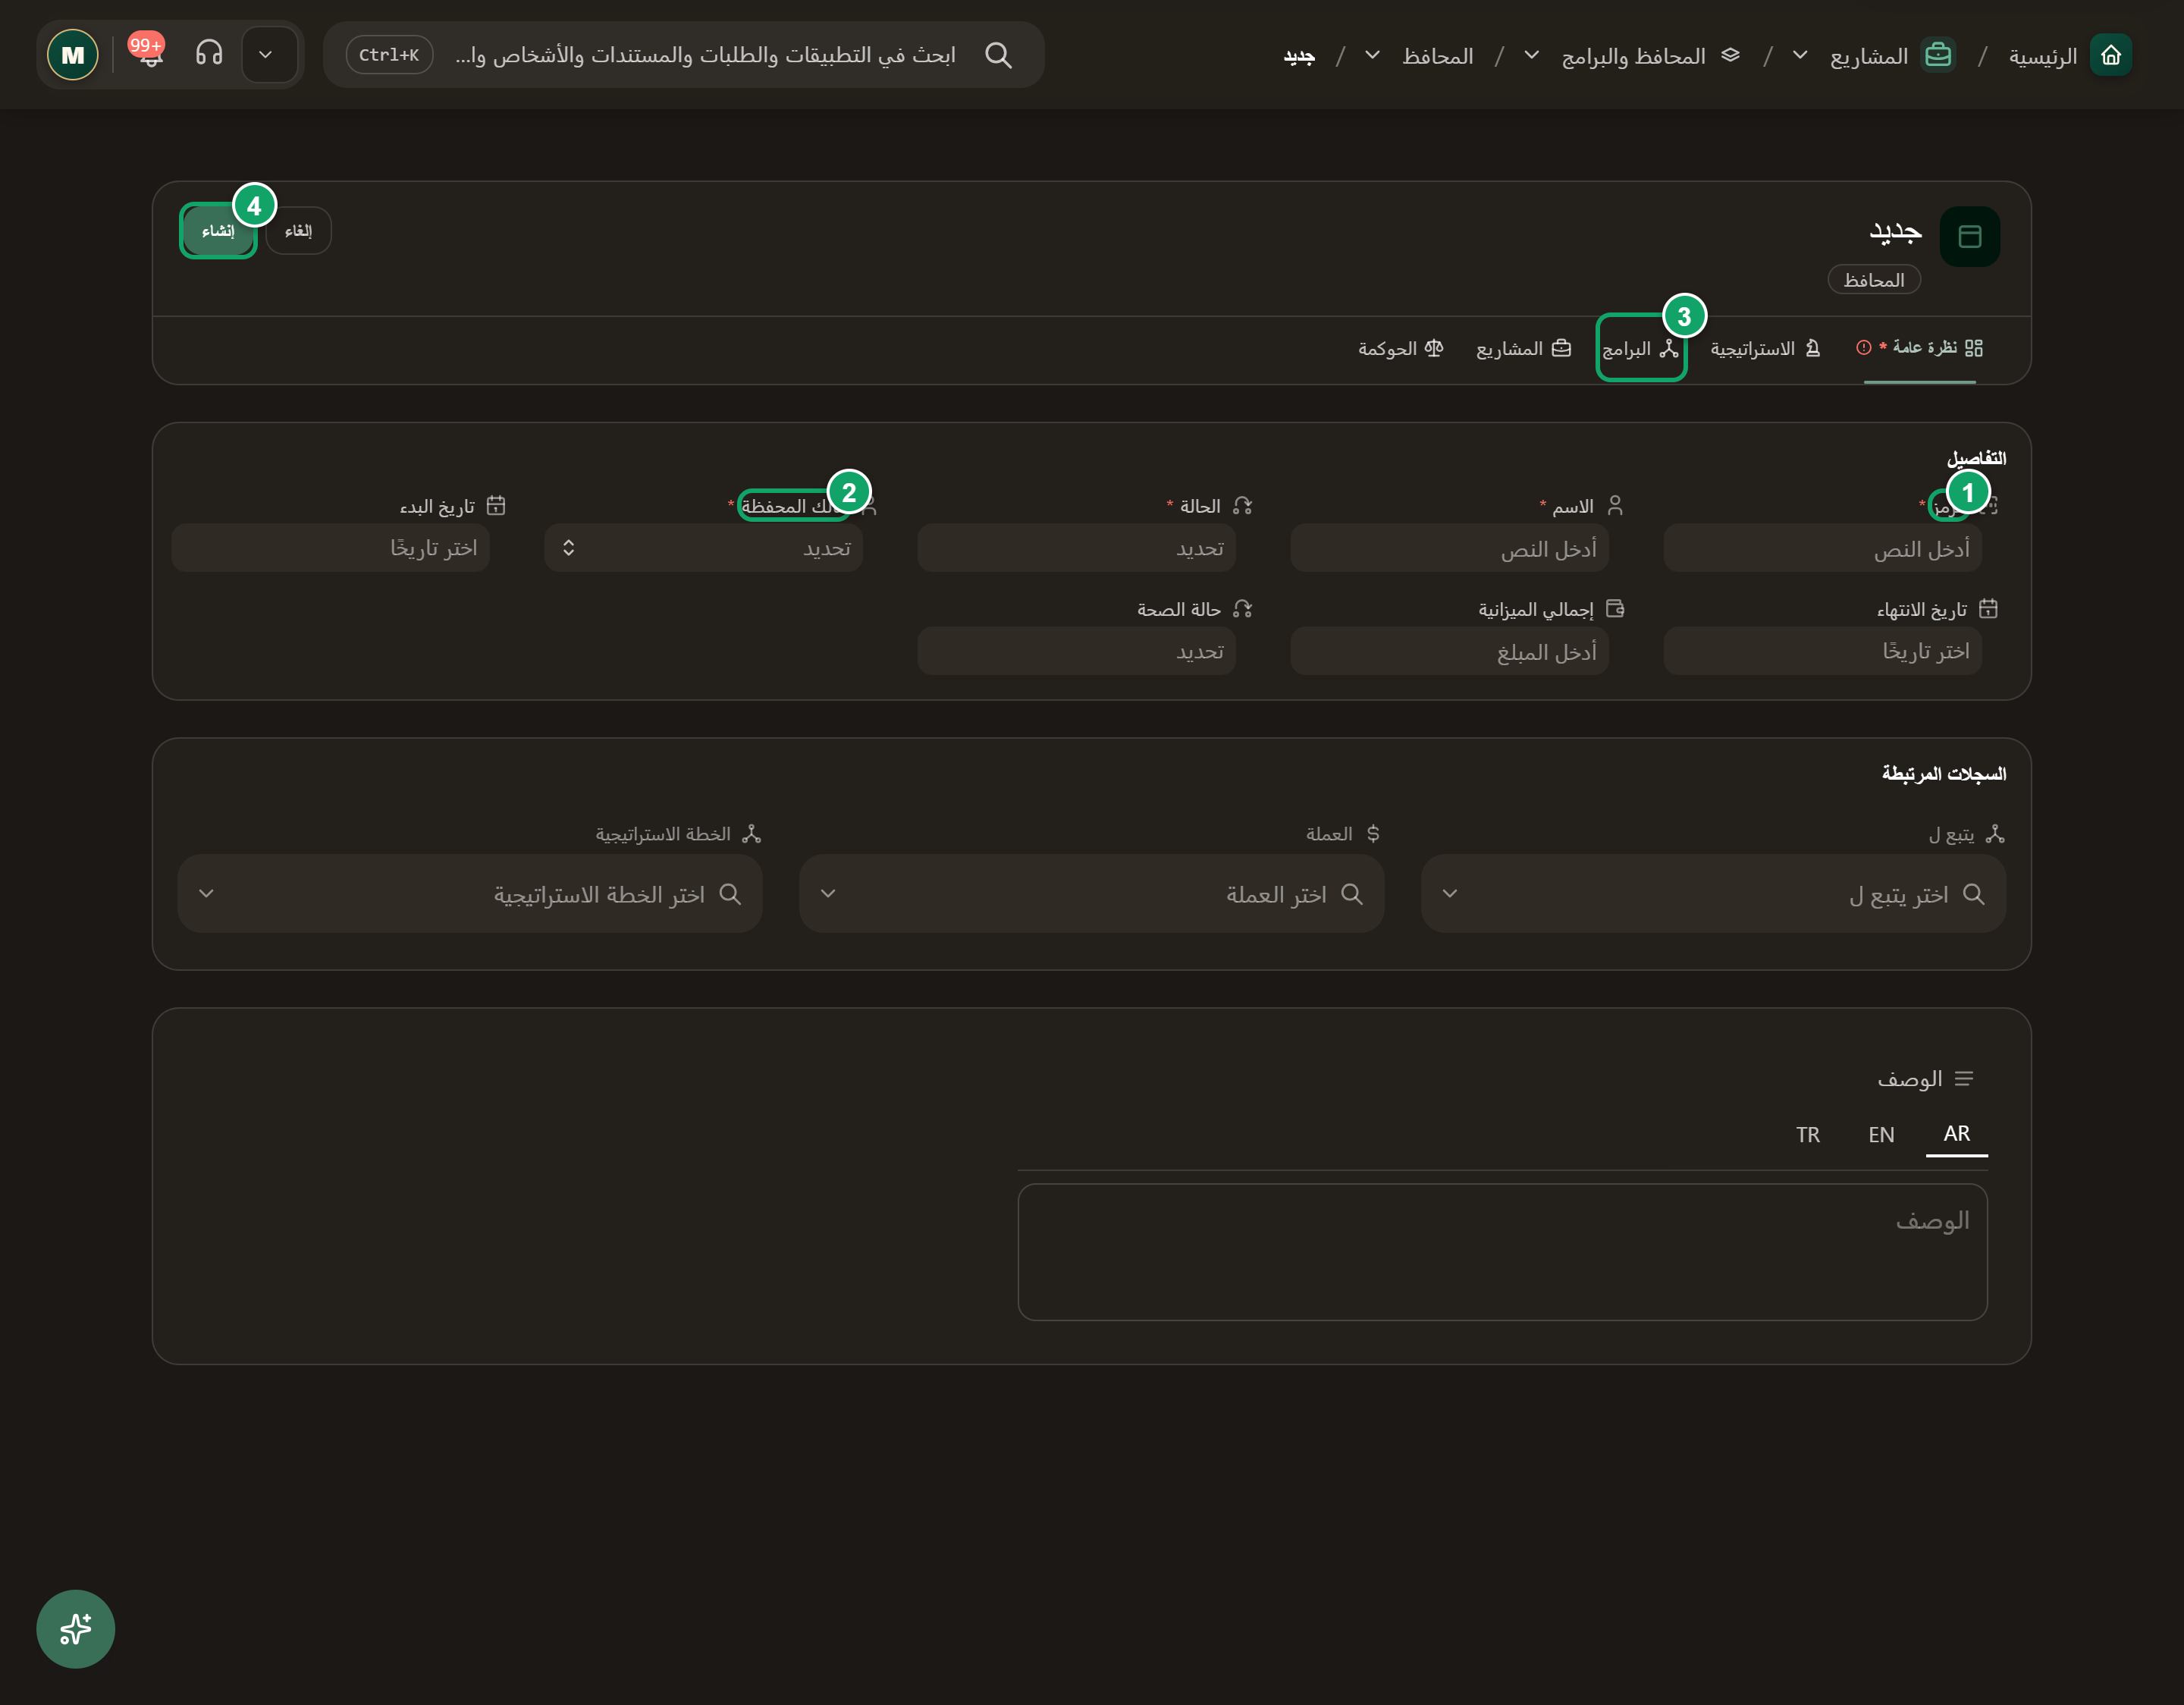
\includegraphics[width=0.95\linewidth,height=0.72\textheight,keepaspectratio]{figures/screens/ch05-portfolios-ar.png}
\caption{نموذج محفظة جديدة قبل الحفظ}
\label{fig:projects-screen-portfolios}
\shotnote{تحدد بيانات المحفظة اسمها ومالكها وحالتها قبل ربط البرامج والمشاريع بها. يظهر الربط بالخطة الاستراتيجية والعملة ضمن البيانات المرتبطة، بينما يبقى إنشاء المحفظة خطوة مستقلة عن إنشاء البرامج التي قد تتبعها. ① «الرمز»: رمز فريد للمحفظة. ② «مالك المحفظة». ③ تبويب «البرامج» الذي يجمع برامج المحفظة. ④ «إنشاء».}
\end{figure}
\begin{table}[H]
\centering
\caption{ما الذي تسجّله؟}
\label{tab:projects-portfolios-fields}
\begin{tabularx}{\linewidth}{R{4.2cm} Y}
\rcHeaderRow
\thh{نوع البيانات} & \thh{الحقول}\\
بيانات إلزامية & «الرمز»، «الاسم»، «الحالة»، «مالك المحفظة».\\
بيانات إضافية & «الوصف»، «التوافق الاستراتيجي»، «تاريخ البدء»، «تاريخ الانتهاء»، «إجمالي الميزانية»، «العملة»، «حالة الصحة»، «طريقة تحديد الأولويات»، «مستوى النضج»، «الخطة الاستراتيجية»، «الوسوم».\\
\end{tabularx}
\end{table}
\begin{table}[H]
\centering
\caption{التبويبات والسجلات المرتبطة}
\label{tab:projects-portfolios-tabs}
\begin{tabularx}{\linewidth}{R{4.2cm} Y}
\rcHeaderRow
\thh{التبويب} & \thh{ما الذي تجده فيه؟}\\
«نظرة عامة» & «ملخص المحفظة»؛ «الجدول الزمني والصحة»\\
«الاستراتيجية» & «المواءمة الاستراتيجية»\\
«البرامج» & البرامج (\ref{sec:projects-feature-programs})\\
«المشاريع» & المشاريع (\ref{sec:projects-feature-projects})\\
«المالية» & يعرض المعلومات المرتبطة بهذا الجانب عندما تنطبق إعدادات السجل.\\
«الحوكمة» & «نموذج الحوكمة»؛ مراجعات التخطيط (\ref{sec:projects-feature-planning-reviews})؛ اعتمادات التخطيط (\ref{sec:projects-feature-planning-approvals})؛ قرارات التخطيط (\ref{sec:projects-feature-planning-decisions})\\
\end{tabularx}
\end{table}
\begin{figure}[H]
\centering
\begin{tikzpicture}[node distance=0.5cm]
\node[stepBox] (n0) {\RL{اختيار صفحة العمل}};
\node[stepBox,below=of n0] (n1) {\RL{المحافظ}};
\node[stepBox,below=of n1] (n2) {\RL{الحفظ ثم إعادة الفتح}};
\draw[flowsTo] (n0) -- (n1);
\draw[flowsTo] (n1) -- (n2);
\end{tikzpicture}
\rclegend
\caption{مسار العمل والتحقق}
\label{fig:projects-portfolios-flow}
\shotnote{يبدأ العمل بفتح «المحافظ» واختيار السجل الصحيح قبل إدخال التفاصيل. إعادة فتحه بعد الحفظ تؤكد بقاء البيانات، لكنها لا تعني اعتمادها أو اكتمال العمل المرتبط بها.}
\end{figure}

\subsection{خطوات العمل والتحقق}
\begin{enumerate}
\item افتح «المحافظ» واضغط «إضافة». أدخل الرمز والاسم واختر الحالة ومالك المحفظة.
\item أكمل معلومات التوجه والتواريخ والميزانية عندما تحتاج إليها، ثم اضغط «إنشاء». لا تعتبر مبلغ الميزانية وحده دليلاً على وجود تمويل متاح.
\item أعد فتح المحفظة وراجع مالكها وحالتها. عند ربط برنامج أو مشروع، اختر هذه المحفظة في السجل المعني ثم تحقق من ظهوره ضمن سجلاتها المرتبطة.
\end{enumerate}

\textbf{تطبيق المثال:} في المثال الافتراضي، استخدم «تطوير فروع الأفق» في «الاسم»، ثم أكمل بقية البيانات بما يناسب عمل الأفق. لا تستخدم قيم المثال بديلاً عن السجلات الفعلية المطلوبة في حقول الربط.

\textbf{تحقق ومعالجة المشكلة:} يجب أن تجد السجل بعد إعادة فتحه وأن تبقى البيانات التي حفظتها. إذا لم يظهر، فراجع البحث والفلاتر والنطاق وصلاحية الوصول قبل إنشائه مرة أخرى. وإذا تعذر الحفظ، فأكمل الحقول المطلوبة ورسائل التحقق؛ أما غياب تبويب أو قفل حقل فيستدعي مراجعة نوع السجل وإطاره ومرحلته مع المسؤول.

\clearpage
\section{البرامج}
\label{sec:projects-feature-programs}

ينسّق البرنامج مشاريع مترابطة لتحقيق فائدة مشتركة. يراجع مدير البرنامج المشاريع والنتائج والموارد معاً، ويمكن ربط البرنامج بمحفظة عند الحاجة.

\begin{rcnote}[مثال: شركة الأفق]
تربط سارة مشروع زيارة حلب ببرنامج «تحسين خدمات الفروع» بعد الاتفاق مع مديره. يظهر المشروع ضمن أعمال البرنامج، فتُراجع فائدته مع بقية المشاريع المرتبطة.
\end{rcnote}

\textbf{المسار ومن يستخدمه:} افتح تطبيق «المشاريع»، ثم بطاقة «البرامج». هذه صفحة رئيسية في التطبيق. يستخدمها المسؤول عن هذا العمل، ويعدّل الموظف البيانات المسموح له بها وفق صلاحياته.

\begin{figure}[H]
\centering
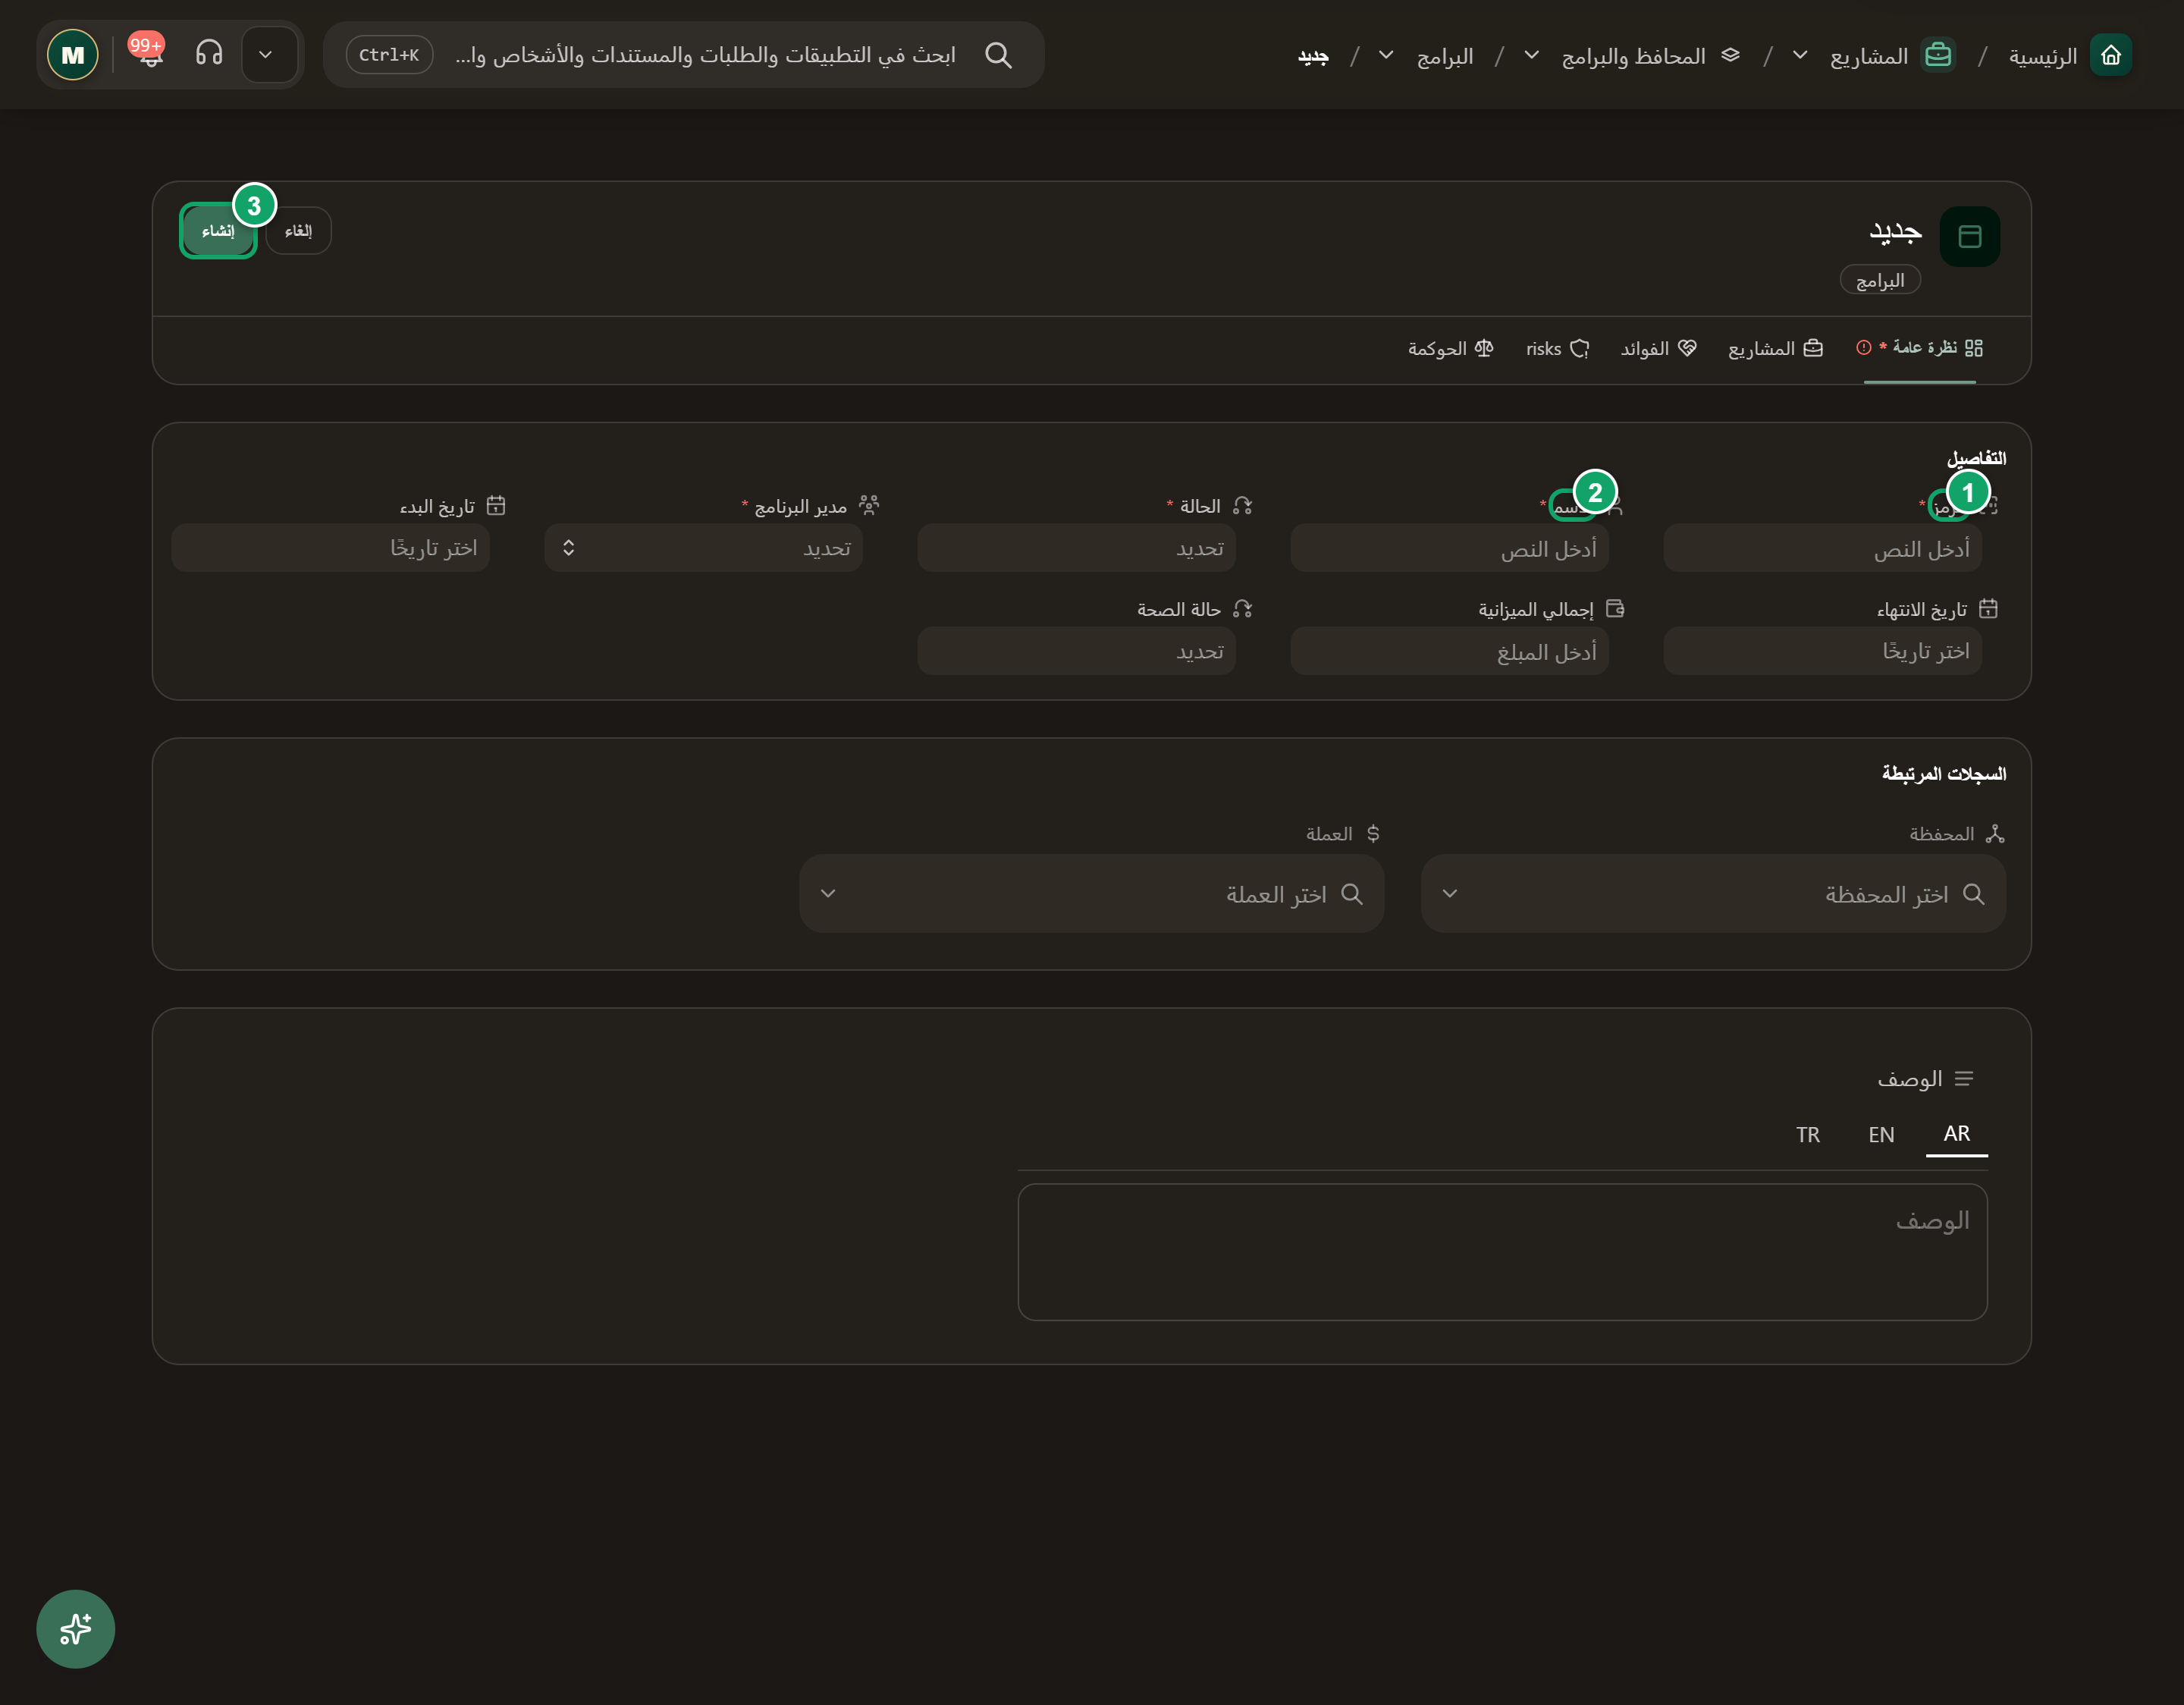
\includegraphics[width=0.95\linewidth,height=0.72\textheight,keepaspectratio]{figures/screens/ch05-programs-ar.png}
\caption{نموذج برنامج جديد قبل الحفظ}
\label{fig:projects-screen-programs}
\shotnote{يعرض النموذج مدير البرنامج وحالته والتواريخ، مع ربط اختياري بالمحفظة. تساعد هذه البيانات على تحديد من ينسّق المشاريع المرتبطة، ولا يعني اختيار محفظة أن المشاريع أُضيفت إلى البرنامج تلقائياً. ① «الرمز» و② «الاسم»: أول حقلين يعرّفان البرنامج. ③ «إنشاء».}
\end{figure}
\begin{table}[H]
\centering
\caption{ما الذي تسجّله؟}
\label{tab:projects-programs-fields}
\begin{tabularx}{\linewidth}{R{4.2cm} Y}
\rcHeaderRow
\thh{نوع البيانات} & \thh{الحقول}\\
بيانات إلزامية & «الرمز»، «الاسم»، «الحالة»، «مدير البرنامج».\\
بيانات إضافية & «الوصف»، «المحفظة»، «الراعي»، «تاريخ البدء»، «تاريخ الانتهاء»، «إجمالي الميزانية»، «العملة»، «حالة الصحة»، «ملخص الفوائد»، «الخطة الاستراتيجية»، «الوسوم».\\
\end{tabularx}
\end{table}
\begin{table}[H]
\centering
\caption{التبويبات والسجلات المرتبطة}
\label{tab:projects-programs-tabs}
\begin{tabularx}{\linewidth}{R{4.2cm} Y}
\rcHeaderRow
\thh{التبويب} & \thh{ما الذي تجده فيه؟}\\
«نظرة عامة» & «ملخص البرنامج»\\
«المشاريع» & المشاريع (\ref{sec:projects-feature-projects})\\
«الفوائد» & «حالة الفوائد»\\
«المالية» & يعرض المعلومات المرتبطة بهذا الجانب عندما تنطبق إعدادات السجل.\\
«التنفيذ» & «سياق التنفيذ»\\
«الحوكمة» & «الحوكمة»؛ مراجعات التخطيط (\ref{sec:projects-feature-planning-reviews})؛ اعتمادات التخطيط (\ref{sec:projects-feature-planning-approvals})؛ قرارات التخطيط (\ref{sec:projects-feature-planning-decisions})\\
\end{tabularx}
\end{table}
\begin{figure}[H]
\centering
\begin{tikzpicture}[node distance=0.5cm]
\node[stepBox] (n0) {\RL{اختيار صفحة العمل}};
\node[stepBox,below=of n0] (n1) {\RL{البرامج}};
\node[stepBox,below=of n1] (n2) {\RL{الحفظ ثم إعادة الفتح}};
\draw[flowsTo] (n0) -- (n1);
\draw[flowsTo] (n1) -- (n2);
\end{tikzpicture}
\rclegend
\caption{مسار العمل والتحقق}
\label{fig:projects-programs-flow}
\shotnote{يبدأ العمل بفتح «البرامج» واختيار السجل الصحيح قبل إدخال التفاصيل. إعادة فتحه بعد الحفظ تؤكد بقاء البيانات، لكنها لا تعني اعتمادها أو اكتمال العمل المرتبط بها.}
\end{figure}

\subsection{خطوات العمل والتحقق}
\begin{enumerate}
\item افتح «البرامج» واضغط «إضافة». أدخل الرمز والاسم واختر الحالة ومدير البرنامج.
\item اختر المحفظة إذا كان البرنامج يتبعها، ثم اكتب الفوائد المتوقعة والتواريخ والمعلومات المالية المتاحة. اضغط «إنشاء».
\item أعد فتح البرنامج وراجع مديره والفوائد التي يتابعها. اربط المشاريع المناسبة من حقل البرنامج في كل مشروع، وتحقق من قائمة المشاريع المرتبطة.
\end{enumerate}

\textbf{تطبيق المثال:} في المثال الافتراضي، استخدم «تحسين خدمات الفروع» في «الاسم»، ثم أكمل بقية البيانات بما يناسب عمل الأفق. لا تستخدم قيم المثال بديلاً عن السجلات الفعلية المطلوبة في حقول الربط.

\textbf{تحقق ومعالجة المشكلة:} يجب أن تجد السجل بعد إعادة فتحه وأن تبقى البيانات التي حفظتها. إذا لم يظهر، فراجع البحث والفلاتر والنطاق وصلاحية الوصول قبل إنشائه مرة أخرى. وإذا تعذر الحفظ، فأكمل الحقول المطلوبة ورسائل التحقق؛ أما غياب تبويب أو قفل حقل فيستدعي مراجعة نوع السجل وإطاره ومرحلته مع المسؤول.

\clearpage
\section{الميزانيات}
\label{sec:projects-feature-budgets}

تجمع الميزانية بنود التكلفة ومصادر التمويل والمصروفات في سجل واحد. يراجع المسؤول المالي المبلغ المخطط وما سُجّل فعلياً قبل اتخاذ قرار بشأن الإنفاق.

\begin{rcnote}[مثال: شركة الأفق]
تنسّق سارة مع المسؤول المالي لإعداد ميزانية زيارة حلب. يسجّل المسؤول بند الانتقال ثم يقارن المبلغ المخطط بالمصروفات المسجّلة للعملة والفترة نفسيهما.
\end{rcnote}

\textbf{المسار ومن يستخدمه:} افتح تطبيق «المشاريع»، ثم بطاقة «الميزانيات». هذه صفحة رئيسية في التطبيق. يستخدمها المسؤول عن هذا العمل، ويعدّل الموظف البيانات المسموح له بها وفق صلاحياته.

\begin{figure}[H]
\centering
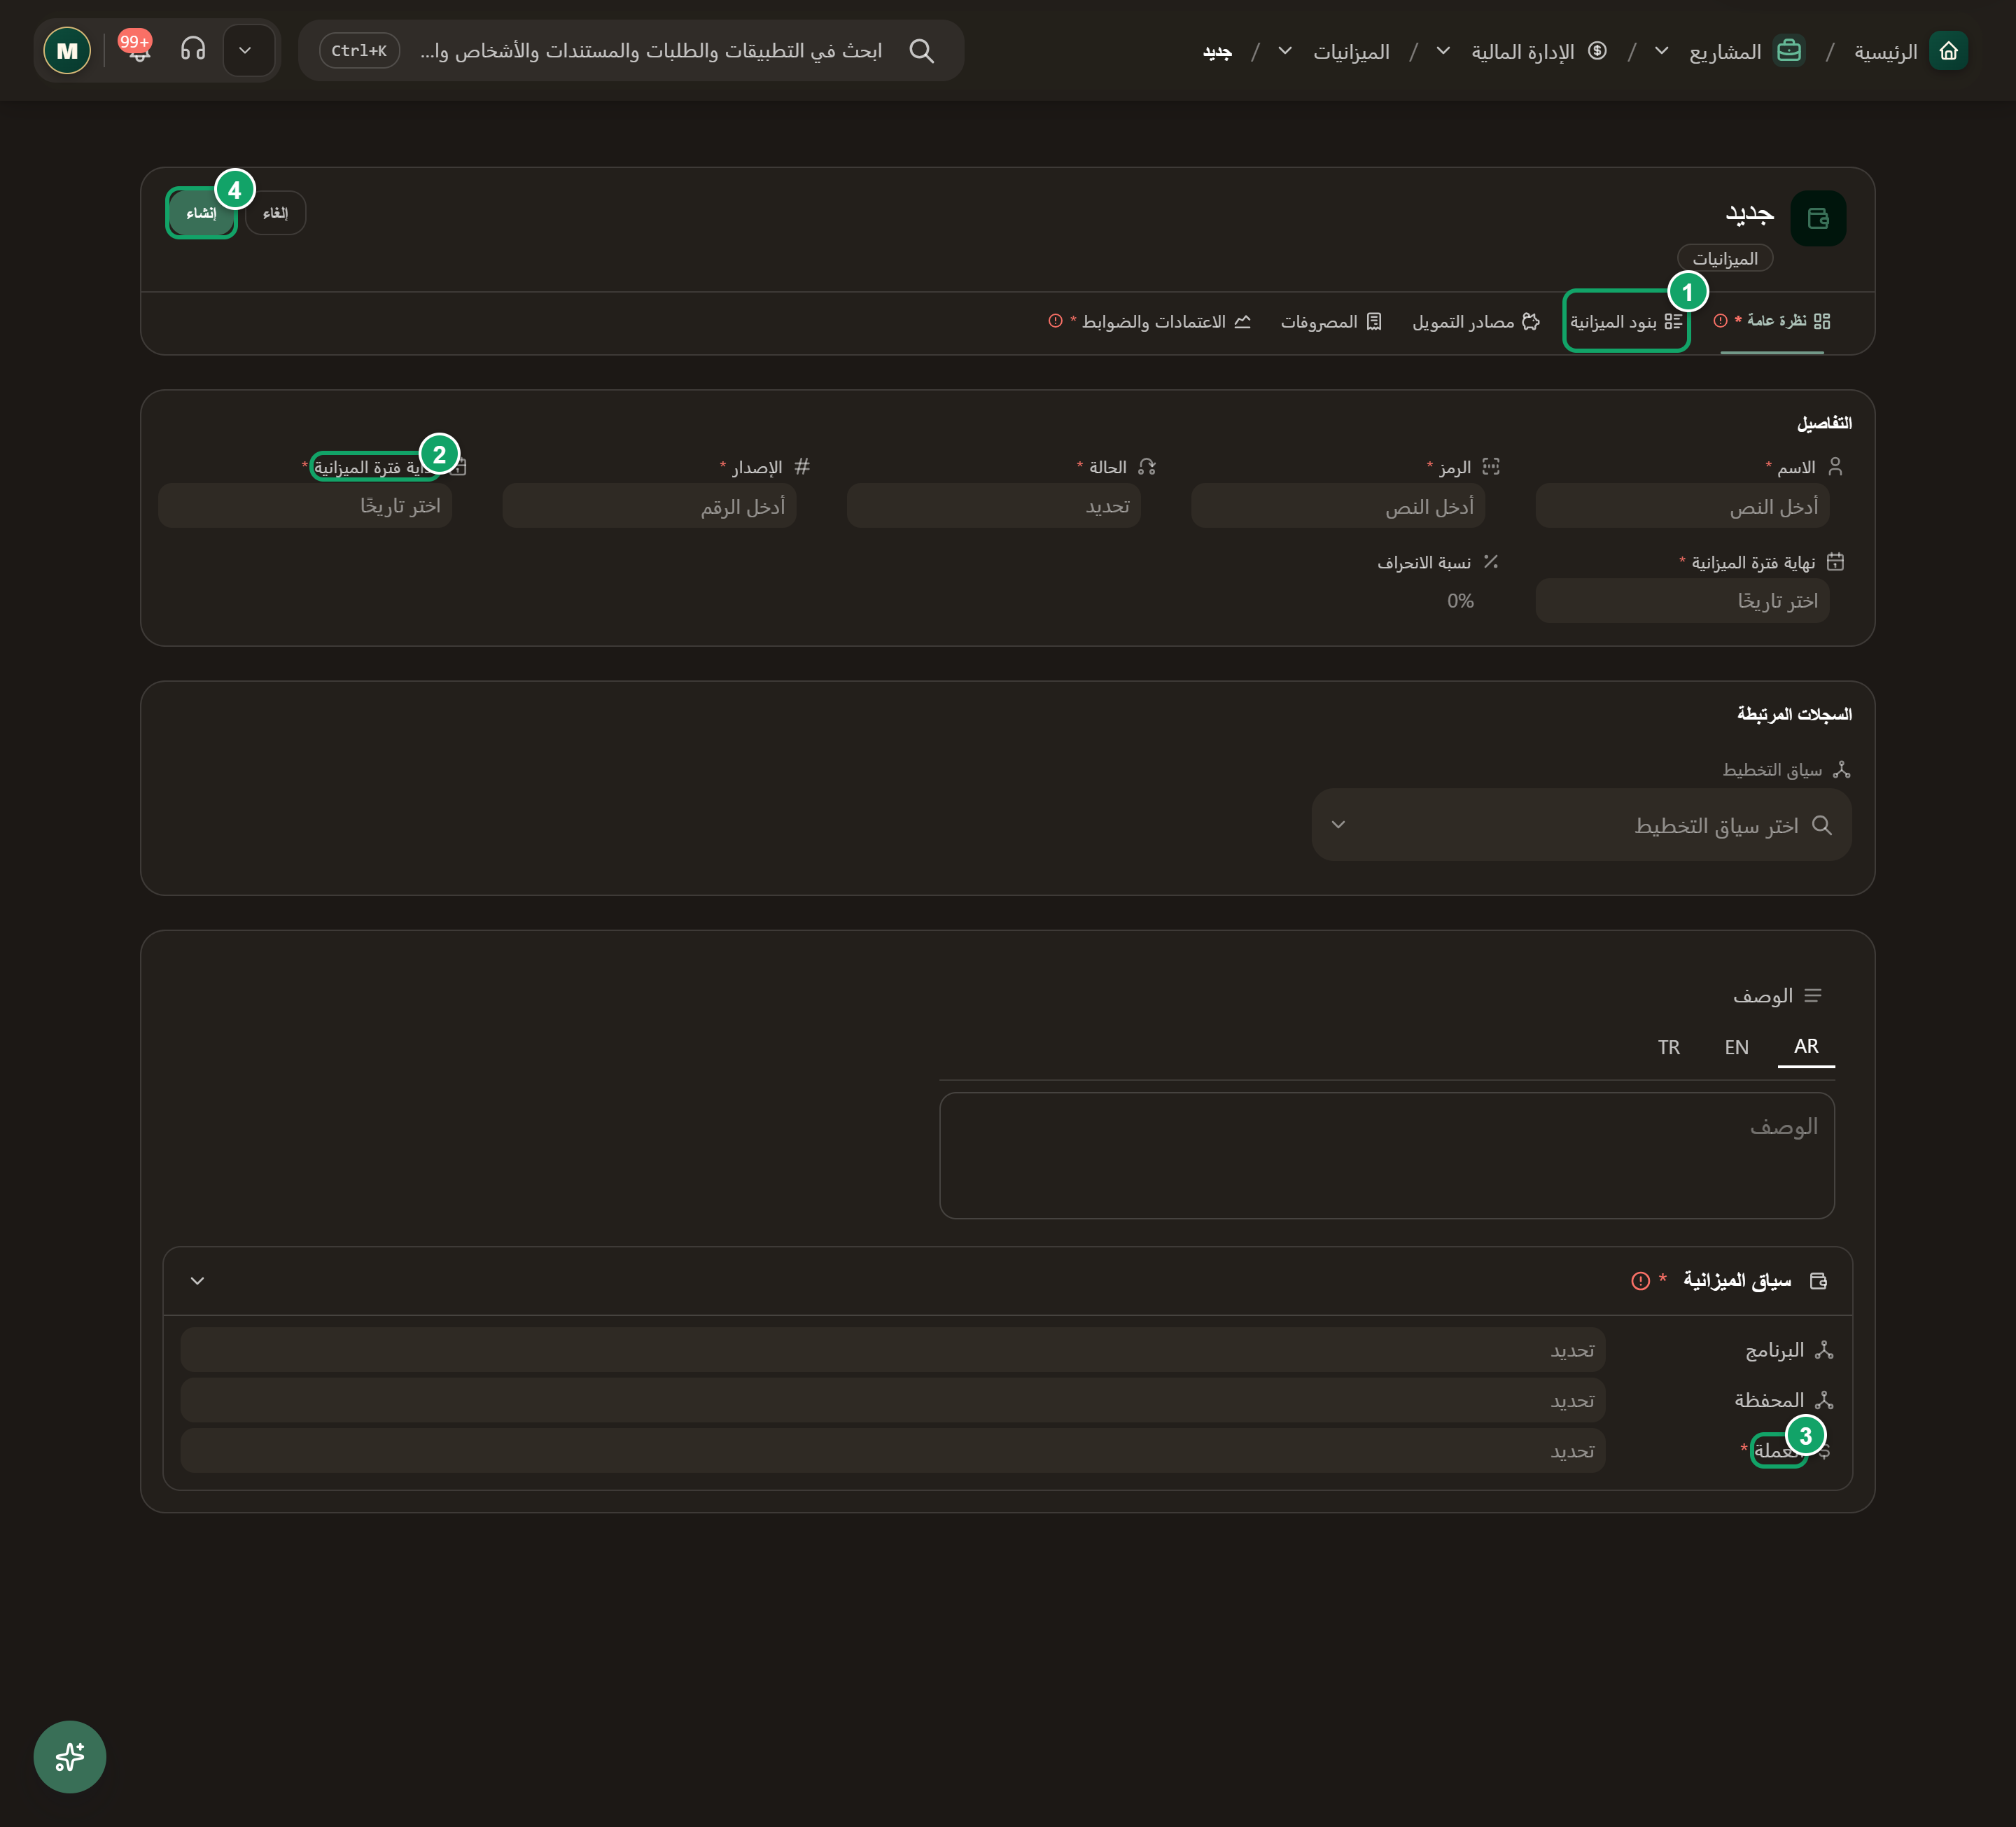
\includegraphics[width=0.95\linewidth,height=0.72\textheight,keepaspectratio]{figures/screens/ch05-budgets-ar.png}
\caption{إعداد ميزانية جديدة قبل الحفظ}
\label{fig:projects-screen-budgets}
\shotnote{يربط النموذج اسم الميزانية وإصدارها بفترة وعملة محددتين، ويتيح اختيار سياق العمل. أما البنود والتمويل والمصروفات فلها أقسامها؛ لذلك لا تمثّل هذه الشاشة وحدها ميزانية مكتملة أو عملية إنفاق. ① تبويب «بنود الميزانية» الذي تُفصَّل فيه المبالغ. ② «بداية فترة الميزانية». ③ «العملة» في سياق الميزانية. ④ «إنشاء».}
\end{figure}
\begin{table}[H]
\centering
\caption{ما الذي تسجّله؟}
\label{tab:projects-budgets-fields}
\begin{tabularx}{\linewidth}{R{4.2cm} Y}
\rcHeaderRow
\thh{نوع البيانات} & \thh{الحقول}\\
بيانات إلزامية & «الاسم»، «الرمز»، «الحالة»، «الإصدار»، «الإصدار الحالي»، «العملة»، «بداية فترة الميزانية»، «نهاية فترة الميزانية»، «أعد بواسطة».\\
بيانات إضافية & «الوصف»، «سياق التخطيط»، «البرنامج»، «المحفظة»، «الإصدار السابق»، «إجمالي المخطط»، «إجمالي الفعلي»، «إجمالي الملتزم»، «إجمالي المتاح»، «إجمالي الممول»، «فجوة التمويل»، «نسبة الانحراف»، «مبلغ الطوارئ»، «نسبة الطوارئ»، «اعتمد بواسطة»، «تاريخ الاعتماد»، «ملاحظات».\\
\end{tabularx}
\end{table}
\begin{table}[H]
\centering
\caption{التبويبات والسجلات المرتبطة}
\label{tab:projects-budgets-tabs}
\begin{tabularx}{\linewidth}{R{4.2cm} Y}
\rcHeaderRow
\thh{التبويب} & \thh{ما الذي تجده فيه؟}\\
«نظرة عامة» & «سياق الميزانية»؛ «إجماليات الميزانية»\\
«بنود الميزانية» & بنود الميزانية (\ref{sec:projects-feature-budget-lines})\\
«مصادر التمويل» & «حالة التمويل»؛ مصادر التمويل (\ref{sec:projects-feature-funding-sources})\\
«المصروفات» & المصروفات (\ref{sec:projects-feature-expenditures})\\
«الاعتمادات والضوابط» & «الإصدارات»؛ «الاعتمادات»؛ «ضوابط التوقع»\\
\end{tabularx}
\end{table}
\begin{figure}[H]
\centering
\begin{tikzpicture}[node distance=0.5cm]
\node[stepBox] (n0) {\RL{اختيار صفحة العمل}};
\node[stepBox,below=of n0] (n1) {\RL{الميزانيات}};
\node[stepBox,below=of n1] (n2) {\RL{الحفظ ثم إعادة الفتح}};
\draw[flowsTo] (n0) -- (n1);
\draw[flowsTo] (n1) -- (n2);
\end{tikzpicture}
\rclegend
\caption{مسار العمل والتحقق}
\label{fig:projects-budgets-flow}
\shotnote{يبدأ العمل بفتح «الميزانيات» واختيار السجل الصحيح قبل إدخال التفاصيل. إعادة فتحه بعد الحفظ تؤكد بقاء البيانات، لكنها لا تعني اعتمادها أو اكتمال العمل المرتبط بها.}
\end{figure}

\subsection{خطوات العمل والتحقق}
\begin{enumerate}
\item افتح «الميزانيات» في تطبيق «المشاريع» واضغط «إضافة». أدخل الرمز والاسم واختر العملة وبداية فترة الميزانية ونهايتها.
\item راجع الحالة والإصدار و«الإصدار الحالي» و«أعد بواسطة». اربط الميزانية بسياق العمل المقصود عند الحاجة، ثم اضغط «إنشاء».
\item أعد فتح الميزانية وأضف بنودها من «بنود الميزانية». راجع نوع كل بند وطريقة احتسابه قبل تفسير الإجمالي.
\item تابع مصادر التمويل والمصروفات في أقسامها. تحقق من الإصدار والعملة والفترة عند المقارنة، ولا تخلط التعهد بالتمويل بالمبلغ المستلم أو المصروف المدفوع.
\end{enumerate}

\textbf{تطبيق المثال:} في المثال الافتراضي، استخدم «ميزانية زيارة فرع حلب» في «الاسم»، ثم أكمل بقية البيانات بما يناسب عمل الأفق. لا تستخدم قيم المثال بديلاً عن السجلات الفعلية المطلوبة في حقول الربط.

\textbf{تحقق ومعالجة المشكلة:} يجب أن تجد السجل بعد إعادة فتحه وأن تبقى البيانات التي حفظتها. إذا لم يظهر، فراجع البحث والفلاتر والنطاق وصلاحية الوصول قبل إنشائه مرة أخرى. وإذا تعذر الحفظ، فأكمل الحقول المطلوبة ورسائل التحقق؛ أما غياب تبويب أو قفل حقل فيستدعي مراجعة نوع السجل وإطاره ومرحلته مع المسؤول.

\clearpage
\section{فئات التكلفة}
\label{sec:projects-feature-cost-categories}

توحّد فئات التكلفة طريقة تصنيف بنود الميزانية، مثل السفر والتجهيزات. يهيّئها المسؤول المالي كي يمكن مقارنة بنود متشابهة بدلاً من توزيعها على تسميات مختلفة.

\begin{rcnote}[مثال: شركة الأفق]
يهيّئ المسؤول المالي فئة «السفر والانتقال» بالرمز \en{HZN-C-01} والنوع «سفر». تستخدم سارة هذه الفئة عند تصنيف بند انتقال فريق الزيارة، فتظل تكاليف السفر مجمّعة تحت تسمية واحدة.
\end{rcnote}

\textbf{المسار ومن يستخدمه:} افتح تطبيق «المشاريع»، ثم بطاقة «فئات التكلفة». هذه صفحة رئيسية في التطبيق. يستخدمها المسؤول عن هذا العمل، ويعدّل الموظف البيانات المسموح له بها وفق صلاحياته.

\begin{figure}[H]
\centering
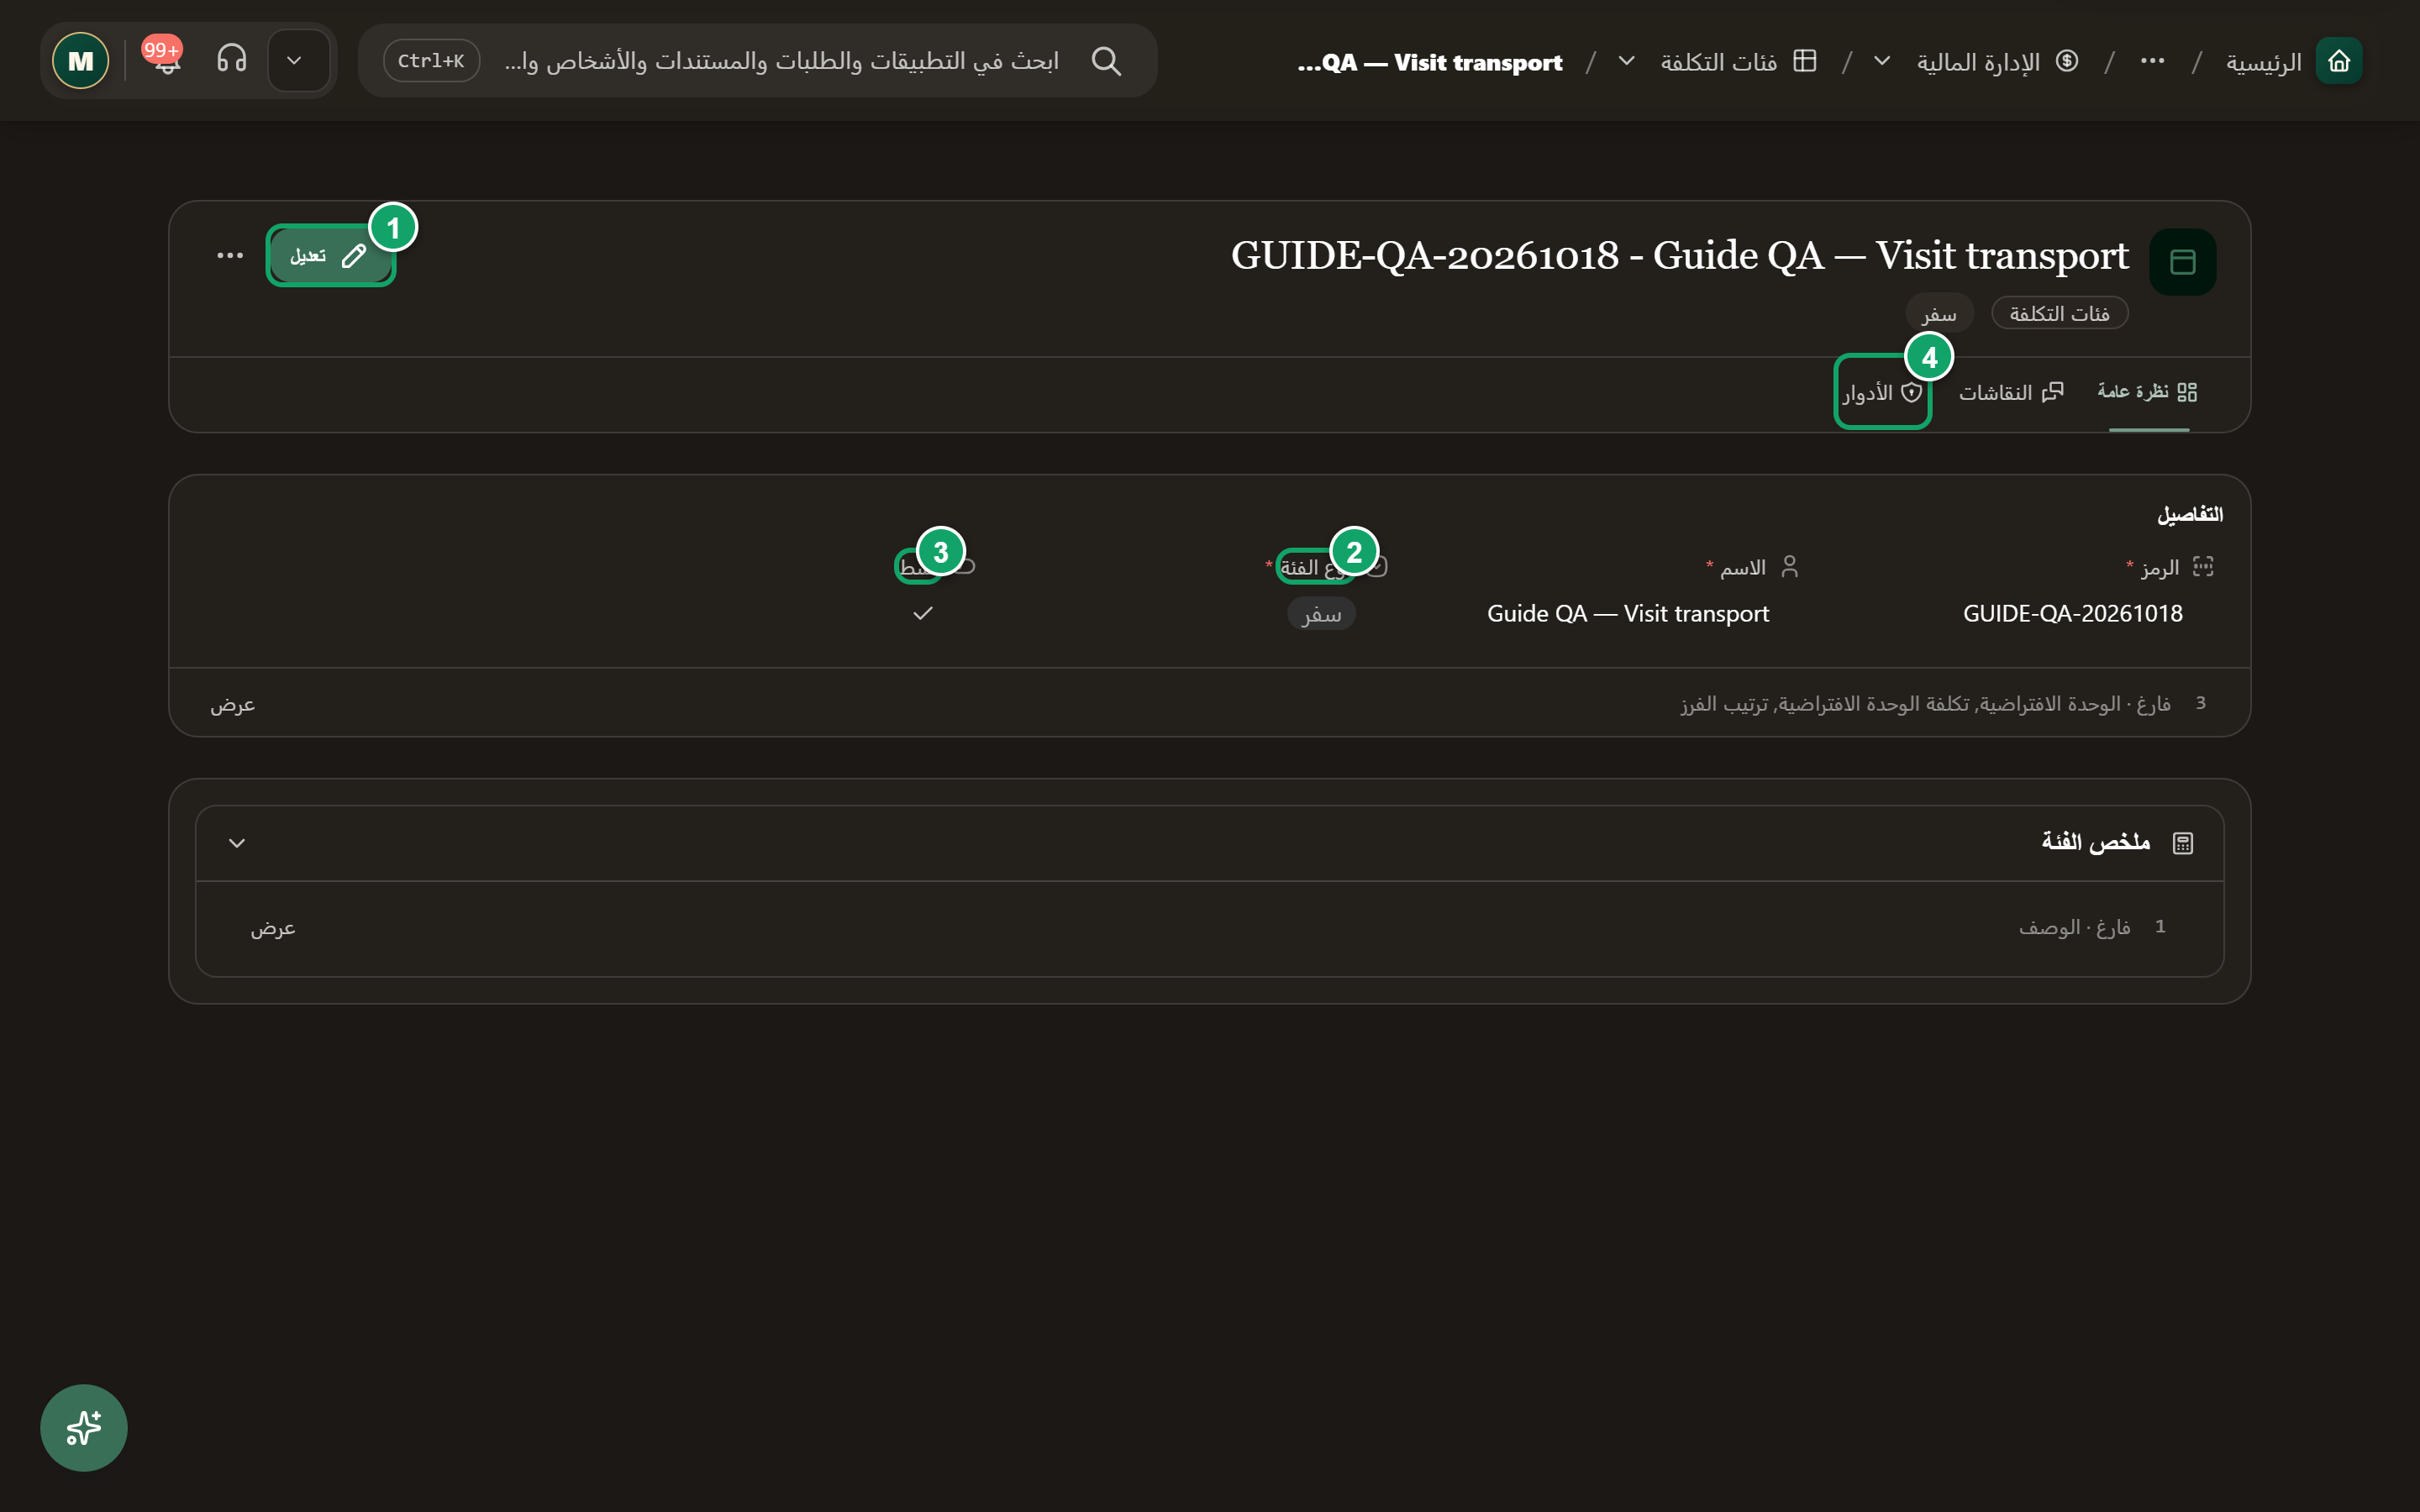
\includegraphics[width=0.95\linewidth,height=0.72\textheight,keepaspectratio]{figures/screens/ch05-cost-category-ar.png}
\caption{فئة تكلفة تجريبية بعد حفظها}
\label{fig:projects-screen-cost-category}
\shotnote{يعرض السجل المحفوظ الرمز والاسم والنوع «سفر»، مع تفعيل الفئة. الحقول الفارغة مخفية ويمكن إظهارها، لذا لا يعني غياب قيمة الوحدة أو تكلفتها أن الحفظ فشل؛ هذا سجل اختبار منفصل عن مثال شركة الأفق. ① «تعديل». ② «نوع الفئة»: يصنّف التكلفة، وهو هنا «سفر». ③ «نشط»: يبيّن أن الفئة متاحة للاستخدام. ④ تبويب «الأدوار» لمن يستطيع رؤية الفئة أو تعديلها.}
\end{figure}
\begin{table}[H]
\centering
\caption{ما الذي تسجّله؟}
\label{tab:projects-cost-categories-fields}
\begin{tabularx}{\linewidth}{R{4.2cm} Y}
\rcHeaderRow
\thh{نوع البيانات} & \thh{الحقول}\\
بيانات إلزامية & «الرمز»، «الاسم»، «نوع الفئة».\\
بيانات إضافية & «الوصف»، «نشط»، «الوحدة الافتراضية»، «تكلفة الوحدة الافتراضية»، «ترتيب الفرز».\\
\end{tabularx}
\end{table}
\begin{table}[H]
\centering
\caption{التبويبات والسجلات المرتبطة}
\label{tab:projects-cost-categories-tabs}
\begin{tabularx}{\linewidth}{R{4.2cm} Y}
\rcHeaderRow
\thh{التبويب} & \thh{ما الذي تجده فيه؟}\\
«نظرة عامة» & «ملخص الفئة»\\
\end{tabularx}
\end{table}
\begin{figure}[H]
\centering
\begin{tikzpicture}[node distance=0.5cm]
\node[stepBox] (n0) {\RL{اختيار صفحة العمل}};
\node[stepBox,below=of n0] (n1) {\RL{فئات التكلفة}};
\node[stepBox,below=of n1] (n2) {\RL{الحفظ ثم إعادة الفتح}};
\draw[flowsTo] (n0) -- (n1);
\draw[flowsTo] (n1) -- (n2);
\end{tikzpicture}
\rclegend
\caption{مسار العمل والتحقق}
\label{fig:projects-cost-categories-flow}
\shotnote{يبدأ العمل بفتح «فئات التكلفة» واختيار السجل الصحيح قبل إدخال التفاصيل. إعادة فتحه بعد الحفظ تؤكد بقاء البيانات، لكنها لا تعني اعتمادها أو اكتمال العمل المرتبط بها.}
\end{figure}

\subsection{خطوات العمل والتحقق}
\begin{enumerate}
\item افتح «فئات التكلفة» واضغط «إضافة». أدخل «الرمز» و«الاسم»، ثم اختر «نوع الفئة».
\item راجع «نشط»، وأدخل الوحدة الافتراضية وتكلفتها إذا كانتا مناسبتين للفئة. اضغط «إنشاء» وانتظر تأكيد النجاح.
\item أعد فتح الفئة من قائمتها. تحقق من الرمز والاسم والنوع، ثم استخدمها في بند الميزانية المناسب بدلاً من إنشاء فئة أخرى بالمعنى نفسه.
\end{enumerate}

\textbf{تطبيق المثال:} في المثال الافتراضي، استخدم «السفر والانتقال» في «الاسم»، ثم أكمل بقية البيانات بما يناسب عمل الأفق. لا تستخدم قيم المثال بديلاً عن السجلات الفعلية المطلوبة في حقول الربط.

\textbf{تحقق ومعالجة المشكلة:} يجب أن تجد السجل بعد إعادة فتحه وأن تبقى البيانات التي حفظتها. إذا لم يظهر، فراجع البحث والفلاتر والنطاق وصلاحية الوصول قبل إنشائه مرة أخرى. وإذا تعذر الحفظ، فأكمل الحقول المطلوبة ورسائل التحقق؛ أما غياب تبويب أو قفل حقل فيستدعي مراجعة نوع السجل وإطاره ومرحلته مع المسؤول.

\clearpage
\section{المحاور التخطيطية}
\label{sec:projects-feature-planning-themes}

يجمع المحور الاستراتيجي مجموعة من الأولويات تحت توجه واضح. استخدمه لتنظيم أهداف الخطة قبل الانتقال إلى تفاصيل التنفيذ.

\begin{rcnote}[مثال: شركة الأفق]
في شركة الأفق، تراجع سارة «جاهزية الفروع» ضمن التحضير لزيارة فرع حلب. تحدد البيانات التي تخص هذا العمل وتتحقق من ظهورها في السجل الصحيح قبل متابعة الخطوة التالية.
\end{rcnote}

\textbf{المسار ومن يستخدمه:} افتح «الخطط» (\ref{sec:projects-feature-plans})، ثم السجل المعني وتبويب «الإطار»، ومنه «المحاور التخطيطية». هذا سجل مرتبط داخل مساحة العمل، وليس صفحة مستقلة في قائمة التطبيق. يستخدمها المسؤول عن هذا العمل، ويعدّل الموظف البيانات المسموح له بها وفق صلاحياته.

\begin{table}[H]
\centering
\caption{ما الذي تسجّله؟}
\label{tab:projects-planning-themes-fields}
\begin{tabularx}{\linewidth}{R{4.2cm} Y}
\rcHeaderRow
\thh{نوع البيانات} & \thh{الحقول}\\
بيانات إلزامية & «العنوان».\\
بيانات إلزامية عند ظهورها & «سياق التخطيط». يعتمد ظهورها على نوع السجل وإعداداته.\\
بيانات إضافية & «الوصف»، «المالك».\\
\end{tabularx}
\end{table}
\begin{figure}[H]
\centering
\begin{tikzpicture}[node distance=0.5cm]
\node[stepBox] (n0) {\RL{المحاور التخطيطية}};
\node[stepBox,below=of n0] (n1) {\RL{سياق التخطيط}};
\draw[dependsOn] (n0) -- (n1);
\end{tikzpicture}
\rclegend
\caption{ارتباط السجل بسياقه}
\label{fig:projects-planning-themes-flow}
\shotnote{يربط حقل «سياق التخطيط» هذا السجل بـأحد سياقات العمل المتاحة. هذا الحقل مطلوب عندما ينطبق النموذج، لذلك جهّز السجل المرجعي قبل الحفظ. قد يكون السياق خطة أو مشروعاً أو برنامجاً أو محفظة بحسب الخيارات المتاحة؛ ولا يلزم إنشاء هذه الأنواع كلها.}
\end{figure}

\subsection{خطوات العمل والتحقق}
\begin{enumerate}
\item افتح السجل المطلوب في «الخطط»، ثم «الإطار». تحقق من الاسم قبل فتح قسم «المحاور التخطيطية».
\item افتح السجل الموجود لتعديله، أو استخدم إجراء الإضافة في القائمة لإنشاء سجل جديد. راجع رابط السجل الأصلي الذي تعبّئه الشاشة، ولا تغيّره دون قصد.
\item أكمل «العنوان». اختر القيم المرتبطة من السجلات الموجودة، وراجع الحقول الإضافية التي تظهر بحسب الاختيارات.
\item عند الإنشاء، اضغط «إنشاء» وانتظر اكتمال الحفظ. أعد فتح السجل من القائمة وتحقق من بياناته وروابطه وحالته.
\end{enumerate}

\textbf{تطبيق المثال:} في المثال الافتراضي، استخدم «جاهزية الفروع» في «العنوان»، ثم أكمل بقية البيانات بما يناسب عمل الأفق. لا تستخدم قيم المثال بديلاً عن السجلات الفعلية المطلوبة في حقول الربط.

\textbf{تحقق ومعالجة المشكلة:} يجب أن تجد السجل بعد إعادة فتحه وأن تبقى البيانات التي حفظتها مرتبطة بسجل «الخطط» المقصود. إذا لم يظهر، فراجع البحث والفلاتر والنطاق وصلاحية الوصول قبل إنشائه مرة أخرى. وإذا تعذر الحفظ، فأكمل الحقول المطلوبة ورسائل التحقق؛ أما غياب تبويب أو قفل حقل فيستدعي مراجعة نوع السجل وإطاره ومرحلته مع المسؤول.

\clearpage
\section{أهداف التخطيط}
\label{sec:projects-feature-planning-objectives}

يصف الهدف التغيير الذي تريد الخطة تحقيقه. اربطه بسياق العمل الصحيح، ثم راجع المؤشرات المرتبطة به بدلاً من الاكتفاء بعنوان عام.

\begin{rcnote}[مثال: شركة الأفق]
في شركة الأفق، تراجع سارة «رفع جاهزية الزيارات» ضمن التحضير لزيارة فرع حلب. تحدد البيانات التي تخص هذا العمل وتتحقق من ظهورها في السجل الصحيح قبل متابعة الخطوة التالية.
\end{rcnote}

\textbf{المسار ومن يستخدمه:} افتح «الخطط» (\ref{sec:projects-feature-plans})، ثم السجل المعني وتبويب «الإطار»، ومنه «أهداف التخطيط». هذا سجل مرتبط داخل مساحة العمل، وليس صفحة مستقلة في قائمة التطبيق. يستخدمها المسؤول عن هذا العمل، ويعدّل الموظف البيانات المسموح له بها وفق صلاحياته.

\begin{table}[H]
\centering
\caption{ما الذي تسجّله؟}
\label{tab:projects-planning-objectives-fields}
\begin{tabularx}{\linewidth}{R{4.2cm} Y}
\rcHeaderRow
\thh{نوع البيانات} & \thh{الحقول}\\
بيانات إلزامية & «الاسم»، «الحالة».\\
بيانات إلزامية عند ظهورها & «سياق التخطيط». يعتمد ظهورها على نوع السجل وإعداداته.\\
بيانات إضافية & «الوصف»، «نوع الهدف»، «الأولوية»، «المالك»، «التاريخ المستهدف».\\
نتائج يحسبها النظام & «نسبة التقدم». راجع بياناتها المصدرية عند اختلاف النتيجة المتوقعة.\\
\end{tabularx}
\end{table}
\begin{figure}[H]
\centering
\begin{tikzpicture}[node distance=0.5cm]
\node[stepBox] (n0) {\RL{أهداف التخطيط}};
\node[stepBox,below=of n0] (n1) {\RL{سياق التخطيط}};
\draw[dependsOn] (n0) -- (n1);
\end{tikzpicture}
\rclegend
\caption{ارتباط السجل بسياقه}
\label{fig:projects-planning-objectives-flow}
\shotnote{يربط حقل «سياق التخطيط» هذا السجل بـأحد سياقات العمل المتاحة. هذا الحقل مطلوب عندما ينطبق النموذج، لذلك جهّز السجل المرجعي قبل الحفظ. قد يكون السياق خطة أو مشروعاً أو برنامجاً أو محفظة بحسب الخيارات المتاحة؛ ولا يلزم إنشاء هذه الأنواع كلها.}
\end{figure}

\subsection{خطوات العمل والتحقق}
\begin{enumerate}
\item افتح السجل المطلوب في «الخطط»، ثم «الإطار». تحقق من الاسم قبل فتح قسم «أهداف التخطيط».
\item افتح السجل الموجود لتعديله، أو استخدم إجراء الإضافة في القائمة لإنشاء سجل جديد. راجع رابط السجل الأصلي الذي تعبّئه الشاشة، ولا تغيّره دون قصد.
\item أكمل «الاسم»، «الحالة». اختر القيم المرتبطة من السجلات الموجودة، وراجع الحقول الإضافية التي تظهر بحسب الاختيارات.
\item عند الإنشاء، اضغط «إنشاء» وانتظر اكتمال الحفظ. أعد فتح السجل من القائمة وتحقق من بياناته وروابطه وحالته.
\end{enumerate}

\textbf{تطبيق المثال:} في المثال الافتراضي، استخدم «رفع جاهزية الزيارات» في «الاسم»، ثم أكمل بقية البيانات بما يناسب عمل الأفق. لا تستخدم قيم المثال بديلاً عن السجلات الفعلية المطلوبة في حقول الربط.

\textbf{تحقق ومعالجة المشكلة:} يجب أن تجد السجل بعد إعادة فتحه وأن تبقى البيانات التي حفظتها مرتبطة بسجل «الخطط» المقصود. إذا لم يظهر، فراجع البحث والفلاتر والنطاق وصلاحية الوصول قبل إنشائه مرة أخرى. وإذا تعذر الحفظ، فأكمل الحقول المطلوبة ورسائل التحقق؛ أما غياب تبويب أو قفل حقل فيستدعي مراجعة نوع السجل وإطاره ومرحلته مع المسؤول.

\clearpage
\section{المبادرات التخطيطية}
\label{sec:projects-feature-planning-initiatives}

تسجّل المبادرة عملاً مقترحاً يدعم التوجه الاستراتيجي. استخدمها لمتابعة الفكرة ومسؤوليتها وحالتها داخل الخطة، دون اعتبار تسجيلها إنشاءً تلقائياً لمشروع.

\begin{rcnote}[مثال: شركة الأفق]
في شركة الأفق، تراجع سارة «توحيد قائمة تجهيز الزيارات» ضمن التحضير لزيارة فرع حلب. تحدد البيانات التي تخص هذا العمل وتتحقق من ظهورها في السجل الصحيح قبل متابعة الخطوة التالية.
\end{rcnote}

\textbf{المسار ومن يستخدمه:} افتح «الخطط» (\ref{sec:projects-feature-plans})، ثم السجل المعني وتبويب «المبادرات»، ومنه «المبادرات التخطيطية». هذا سجل مرتبط داخل مساحة العمل، وليس صفحة مستقلة في قائمة التطبيق. يستخدمها المسؤول عن هذا العمل، ويعدّل الموظف البيانات المسموح له بها وفق صلاحياته.

\begin{table}[H]
\centering
\caption{ما الذي تسجّله؟}
\label{tab:projects-planning-initiatives-fields}
\begin{tabularx}{\linewidth}{R{4.2cm} Y}
\rcHeaderRow
\thh{نوع البيانات} & \thh{الحقول}\\
بيانات إلزامية & «العنوان»، «الحالة».\\
بيانات إلزامية عند ظهورها & «سياق التخطيط». يعتمد ظهورها على نوع السجل وإعداداته.\\
بيانات إضافية & «المحور»، «الهدف»، «الوصف»، «المالك»، «الأولوية»، «البداية المخططة»، «النهاية المخططة»، «فرضية المنفعة»، «الجهة المرتبطة».\\
\end{tabularx}
\end{table}
\begin{figure}[H]
\centering
\begin{tikzpicture}[node distance=0.5cm]
\node[stepBox] (n0) {\RL{المبادرات التخطيطية}};
\node[stepBox,below=of n0] (n1) {\RL{سياق التخطيط}};
\draw[dependsOn] (n0) -- (n1);
\end{tikzpicture}
\rclegend
\caption{ارتباط السجل بسياقه}
\label{fig:projects-planning-initiatives-flow}
\shotnote{يربط حقل «سياق التخطيط» هذا السجل بـأحد سياقات العمل المتاحة. هذا الحقل مطلوب عندما ينطبق النموذج، لذلك جهّز السجل المرجعي قبل الحفظ. قد يكون السياق خطة أو مشروعاً أو برنامجاً أو محفظة بحسب الخيارات المتاحة؛ ولا يلزم إنشاء هذه الأنواع كلها.}
\end{figure}

\subsection{خطوات العمل والتحقق}
\begin{enumerate}
\item افتح السجل المطلوب في «الخطط»، ثم «المبادرات». تحقق من الاسم قبل فتح قسم «المبادرات التخطيطية».
\item افتح السجل الموجود لتعديله، أو استخدم إجراء الإضافة في القائمة لإنشاء سجل جديد. راجع رابط السجل الأصلي الذي تعبّئه الشاشة، ولا تغيّره دون قصد.
\item أكمل «العنوان»، «الحالة». اختر القيم المرتبطة من السجلات الموجودة، وراجع الحقول الإضافية التي تظهر بحسب الاختيارات.
\item عند الإنشاء، اضغط «إنشاء» وانتظر اكتمال الحفظ. أعد فتح السجل من القائمة وتحقق من بياناته وروابطه وحالته.
\end{enumerate}

\textbf{تطبيق المثال:} في المثال الافتراضي، استخدم «توحيد قائمة تجهيز الزيارات» في «العنوان»، ثم أكمل بقية البيانات بما يناسب عمل الأفق. لا تستخدم قيم المثال بديلاً عن السجلات الفعلية المطلوبة في حقول الربط.

\textbf{تحقق ومعالجة المشكلة:} يجب أن تجد السجل بعد إعادة فتحه وأن تبقى البيانات التي حفظتها مرتبطة بسجل «الخطط» المقصود. إذا لم يظهر، فراجع البحث والفلاتر والنطاق وصلاحية الوصول قبل إنشائه مرة أخرى. وإذا تعذر الحفظ، فأكمل الحقول المطلوبة ورسائل التحقق؛ أما غياب تبويب أو قفل حقل فيستدعي مراجعة نوع السجل وإطاره ومرحلته مع المسؤول.

\clearpage
\section{دورات OKR}
\label{sec:projects-feature-planning-okrs}

تجمع دورة الأهداف والنتائج الرئيسية أهداف فترة محددة والنتائج التي تقيس تحققها. حدّد الدورة أولاً، ثم أضف النتائج الرئيسية وتحديثاتها.

\begin{rcnote}[مثال: شركة الأفق]
في شركة الأفق، تراجع سارة «جاهزية الفروع للربع الأخير» ضمن التحضير لزيارة فرع حلب. تحدد البيانات التي تخص هذا العمل وتتحقق من ظهورها في السجل الصحيح قبل متابعة الخطوة التالية.
\end{rcnote}

\textbf{المسار ومن يستخدمه:} افتح «الخطط» (\ref{sec:projects-feature-plans})، ثم السجل المعني وتبويب «الإطار»، ومنه «دورات OKR». هذا سجل مرتبط داخل مساحة العمل، وليس صفحة مستقلة في قائمة التطبيق. يستخدمها المسؤول عن هذا العمل، ويعدّل الموظف البيانات المسموح له بها وفق صلاحياته.

\begin{table}[H]
\centering
\caption{ما الذي تسجّله؟}
\label{tab:projects-planning-okrs-fields}
\begin{tabularx}{\linewidth}{R{4.2cm} Y}
\rcHeaderRow
\thh{نوع البيانات} & \thh{الحقول}\\
بيانات إلزامية & «اسم الدورة».\\
بيانات إلزامية عند ظهورها & «سياق التخطيط». يعتمد ظهورها على نوع السجل وإعداداته.\\
بيانات إضافية & «الهدف»، «الوتيرة»، «المالك».\\
\end{tabularx}
\end{table}
\begin{table}[H]
\centering
\caption{السجلات المرتبطة}
\label{tab:projects-planning-okrs-children}
\begin{tabularx}{\linewidth}{R{4.2cm} Y}
\rcHeaderRow
\thh{السجل} & \thh{افتح الشرح}\\
النتائج الرئيسية & \ref{sec:projects-feature-planning-key-results}\\
\end{tabularx}
\end{table}
\begin{figure}[H]
\centering
\begin{tikzpicture}[node distance=0.5cm]
\node[stepBox] (n0) {\RL{دورات OKR}};
\node[stepBox,below=of n0] (n1) {\RL{سياق التخطيط}};
\draw[dependsOn] (n0) -- (n1);
\end{tikzpicture}
\rclegend
\caption{ارتباط السجل بسياقه}
\label{fig:projects-planning-okrs-flow}
\shotnote{يربط حقل «سياق التخطيط» هذا السجل بـأحد سياقات العمل المتاحة. هذا الحقل مطلوب عندما ينطبق النموذج، لذلك جهّز السجل المرجعي قبل الحفظ. قد يكون السياق خطة أو مشروعاً أو برنامجاً أو محفظة بحسب الخيارات المتاحة؛ ولا يلزم إنشاء هذه الأنواع كلها.}
\end{figure}

\subsection{خطوات العمل والتحقق}
\begin{enumerate}
\item افتح السجل المطلوب في «الخطط»، ثم «الإطار». تحقق من الاسم قبل فتح قسم «دورات OKR».
\item افتح السجل الموجود لتعديله، أو استخدم إجراء الإضافة في القائمة لإنشاء سجل جديد. راجع رابط السجل الأصلي الذي تعبّئه الشاشة، ولا تغيّره دون قصد.
\item أكمل «اسم الدورة». اختر القيم المرتبطة من السجلات الموجودة، وراجع الحقول الإضافية التي تظهر بحسب الاختيارات.
\item عند الإنشاء، اضغط «إنشاء» وانتظر اكتمال الحفظ. أعد فتح السجل من القائمة وتحقق من بياناته وروابطه وحالته.
\end{enumerate}

\textbf{تطبيق المثال:} في المثال الافتراضي، استخدم «جاهزية الفروع للربع الأخير» في «اسم الدورة»، ثم أكمل بقية البيانات بما يناسب عمل الأفق. لا تستخدم قيم المثال بديلاً عن السجلات الفعلية المطلوبة في حقول الربط.

\textbf{تحقق ومعالجة المشكلة:} يجب أن تجد السجل بعد إعادة فتحه وأن تبقى البيانات التي حفظتها مرتبطة بسجل «الخطط» المقصود. إذا لم يظهر، فراجع البحث والفلاتر والنطاق وصلاحية الوصول قبل إنشائه مرة أخرى. وإذا تعذر الحفظ، فأكمل الحقول المطلوبة ورسائل التحقق؛ أما غياب تبويب أو قفل حقل فيستدعي مراجعة نوع السجل وإطاره ومرحلته مع المسؤول.

\clearpage
\section{النتائج الرئيسية}
\label{sec:projects-feature-planning-key-results}

تحوّل النتيجة الرئيسية الهدف إلى نتيجة قابلة للمتابعة. اختر طريقة التتبع المناسبة، وميّز بين القيمة المستهدفة وما تحقق فعلياً.

\begin{rcnote}[مثال: شركة الأفق]
في شركة الأفق، تراجع سارة «اكتمال تجهيز الزيارة» ضمن التحضير لزيارة فرع حلب. تحدد البيانات التي تخص هذا العمل وتتحقق من ظهورها في السجل الصحيح قبل متابعة الخطوة التالية.
\end{rcnote}

\textbf{المسار ومن يستخدمه:} افتح «الخطط» (\ref{sec:projects-feature-plans})، ثم السجل المعني وتبويب «الإطار»، ومنه «النتائج الرئيسية». هذا سجل مرتبط داخل مساحة العمل، وليس صفحة مستقلة في قائمة التطبيق. يستخدمها المسؤول عن هذا العمل، ويعدّل الموظف البيانات المسموح له بها وفق صلاحياته.

\begin{table}[H]
\centering
\caption{ما الذي تسجّله؟}
\label{tab:projects-planning-key-results-fields}
\begin{tabularx}{\linewidth}{R{4.2cm} Y}
\rcHeaderRow
\thh{نوع البيانات} & \thh{الحقول}\\
بيانات إلزامية & «دورة OKR»، «وضع التتبع»، «الاسم»، «نوع الالتزام».\\
بيانات إلزامية عند ظهورها & «سياق التخطيط». يعتمد ظهورها على نوع السجل وإعداداته.\\
بيانات إضافية & «المؤشر»، «طريقة التقييم»، «القيمة المستهدفة»، «قيمة البداية»، «القيمة المستهدفة (رقم)»، «الثقة»، «حالة الوتيرة»، «الحالة».\\
نتائج يحسبها النظام & «القيمة الحالية»، «القيمة الحالية (رقم)»، «نسبة التقييم»، «آخر متابعة». راجع بياناتها المصدرية عند اختلاف النتيجة المتوقعة.\\
\end{tabularx}
\end{table}
\begin{figure}[H]
\centering
\begin{tikzpicture}[node distance=0.5cm]
\node[stepBox] (n0) {\RL{النتائج الرئيسية}};
\node[stepBox,below=of n0] (n1) {\RL{سياق التخطيط}};
\draw[dependsOn] (n0) -- (n1);
\end{tikzpicture}
\rclegend
\caption{ارتباط السجل بسياقه}
\label{fig:projects-planning-key-results-flow}
\shotnote{يربط حقل «سياق التخطيط» هذا السجل بـأحد سياقات العمل المتاحة. هذا الحقل مطلوب عندما ينطبق النموذج، لذلك جهّز السجل المرجعي قبل الحفظ. قد يكون السياق خطة أو مشروعاً أو برنامجاً أو محفظة بحسب الخيارات المتاحة؛ ولا يلزم إنشاء هذه الأنواع كلها.}
\end{figure}

\subsection{خطوات العمل والتحقق}
\begin{enumerate}
\item افتح السجل المطلوب في «الخطط»، ثم «الإطار». تحقق من الاسم قبل فتح قسم «النتائج الرئيسية».
\item افتح السجل الموجود لتعديله، أو استخدم إجراء الإضافة في القائمة لإنشاء سجل جديد. راجع رابط السجل الأصلي الذي تعبّئه الشاشة، ولا تغيّره دون قصد.
\item أكمل «دورة OKR»، «وضع التتبع»، «الاسم»، «نوع الالتزام». اختر القيم المرتبطة من السجلات الموجودة، وراجع الحقول الإضافية التي تظهر بحسب الاختيارات.
\item عند الإنشاء، اضغط «إنشاء» وانتظر اكتمال الحفظ. أعد فتح السجل من القائمة وتحقق من بياناته وروابطه وحالته.
\end{enumerate}

\textbf{تطبيق المثال:} في المثال الافتراضي، استخدم «اكتمال تجهيز الزيارة» في «الاسم»، ثم أكمل بقية البيانات بما يناسب عمل الأفق. لا تستخدم قيم المثال بديلاً عن السجلات الفعلية المطلوبة في حقول الربط.

\textbf{تحقق ومعالجة المشكلة:} يجب أن تجد السجل بعد إعادة فتحه وأن تبقى البيانات التي حفظتها مرتبطة بسجل «الخطط» المقصود. إذا لم يظهر، فراجع البحث والفلاتر والنطاق وصلاحية الوصول قبل إنشائه مرة أخرى. وإذا تعذر الحفظ، فأكمل الحقول المطلوبة ورسائل التحقق؛ أما غياب تبويب أو قفل حقل فيستدعي مراجعة نوع السجل وإطاره ومرحلته مع المسؤول.

\clearpage
\section{متابعات النتائج الرئيسية}
\label{sec:projects-feature-planning-key-result-checkins}

يسجّل تحديث النتيجة الرئيسية وضعها في تاريخ محدد. تساعد التحديثات المتتابعة على فهم التقدم والعوائق بدلاً من الاعتماد على آخر رقم وحده.

\begin{rcnote}[مثال: شركة الأفق]
في شركة الأفق، تراجع سارة «مراجعة جاهزية قائمة الزيارة» ضمن التحضير لزيارة فرع حلب. تحدد البيانات التي تخص هذا العمل وتتحقق من ظهورها في السجل الصحيح قبل متابعة الخطوة التالية.
\end{rcnote}

\textbf{المسار ومن يستخدمه:} افتح «الخطط» (\ref{sec:projects-feature-plans})، ثم السجل المعني وتبويب «الإطار»، ومنه «متابعات النتائج الرئيسية». هذا سجل مرتبط داخل مساحة العمل، وليس صفحة مستقلة في قائمة التطبيق. يستخدمها المسؤول عن هذا العمل، ويعدّل الموظف البيانات المسموح له بها وفق صلاحياته.

\begin{table}[H]
\centering
\caption{ما الذي تسجّله؟}
\label{tab:projects-planning-key-result-checkins-fields}
\begin{tabularx}{\linewidth}{R{4.2cm} Y}
\rcHeaderRow
\thh{نوع البيانات} & \thh{الحقول}\\
بيانات إلزامية & «النتيجة الرئيسية»، «تاريخ المتابعة»، «الحالة».\\
بيانات إلزامية عند ظهورها & «سياق التخطيط». يعتمد ظهورها على نوع السجل وإعداداته.\\
بيانات إضافية & «القيمة (رقم)»، «القيمة (نص)»، «نسبة التقييم»، «الثقة»، «الملخص».\\
\end{tabularx}
\end{table}
\begin{figure}[H]
\centering
\begin{tikzpicture}[node distance=0.5cm]
\node[stepBox] (n0) {\RL{متابعات النتائج الرئيسية}};
\node[stepBox,below=of n0] (n1) {\RL{سياق التخطيط}};
\draw[dependsOn] (n0) -- (n1);
\end{tikzpicture}
\rclegend
\caption{ارتباط السجل بسياقه}
\label{fig:projects-planning-key-result-checkins-flow}
\shotnote{يربط حقل «سياق التخطيط» هذا السجل بـأحد سياقات العمل المتاحة. هذا الحقل مطلوب عندما ينطبق النموذج، لذلك جهّز السجل المرجعي قبل الحفظ. قد يكون السياق خطة أو مشروعاً أو برنامجاً أو محفظة بحسب الخيارات المتاحة؛ ولا يلزم إنشاء هذه الأنواع كلها.}
\end{figure}

\subsection{خطوات العمل والتحقق}
\begin{enumerate}
\item افتح السجل المطلوب في «الخطط»، ثم «الإطار». تحقق من الاسم قبل فتح قسم «متابعات النتائج الرئيسية».
\item افتح السجل الموجود لتعديله، أو استخدم إجراء الإضافة في القائمة لإنشاء سجل جديد. راجع رابط السجل الأصلي الذي تعبّئه الشاشة، ولا تغيّره دون قصد.
\item أكمل «النتيجة الرئيسية»، «تاريخ المتابعة»، «الحالة». اختر القيم المرتبطة من السجلات الموجودة، وراجع الحقول الإضافية التي تظهر بحسب الاختيارات.
\item عند الإنشاء، اضغط «إنشاء» وانتظر اكتمال الحفظ. أعد فتح السجل من القائمة وتحقق من بياناته وروابطه وحالته.
\end{enumerate}

\textbf{تحقق ومعالجة المشكلة:} يجب أن تجد السجل بعد إعادة فتحه وأن تبقى البيانات التي حفظتها مرتبطة بسجل «الخطط» المقصود. إذا لم يظهر، فراجع البحث والفلاتر والنطاق وصلاحية الوصول قبل إنشائه مرة أخرى. وإذا تعذر الحفظ، فأكمل الحقول المطلوبة ورسائل التحقق؛ أما غياب تبويب أو قفل حقل فيستدعي مراجعة نوع السجل وإطاره ومرحلته مع المسؤول.

\clearpage
\section{عناصر هوشين}
\label{sec:projects-feature-planning-hoshin-items}

يربط أسلوب هوشين التوجهات طويلة المدى بالأهداف السنوية والعمل المطلوب. سجّل نوع العنصر بوضوح كي لا تختلط النتيجة الاستراتيجية بالإجراء التنفيذي.

\begin{rcnote}[مثال: شركة الأفق]
في شركة الأفق، تراجع سارة «تحسين انضباط الزيارات» ضمن التحضير لزيارة فرع حلب. تحدد البيانات التي تخص هذا العمل وتتحقق من ظهورها في السجل الصحيح قبل متابعة الخطوة التالية.
\end{rcnote}

\textbf{المسار ومن يستخدمه:} افتح «الخطط» (\ref{sec:projects-feature-plans})، ثم السجل المعني وتبويب «الإطار»، ومنه «عناصر هوشين». هذا سجل مرتبط داخل مساحة العمل، وليس صفحة مستقلة في قائمة التطبيق. يستخدمها المسؤول عن هذا العمل، ويعدّل الموظف البيانات المسموح له بها وفق صلاحياته.

\begin{table}[H]
\centering
\caption{ما الذي تسجّله؟}
\label{tab:projects-planning-hoshin-items-fields}
\begin{tabularx}{\linewidth}{R{4.2cm} Y}
\rcHeaderRow
\thh{نوع البيانات} & \thh{الحقول}\\
بيانات إلزامية & «اسم العنصر»، «نوع العنصر».\\
بيانات إلزامية عند ظهورها & «سياق التخطيط». يعتمد ظهورها على نوع السجل وإعداداته.\\
بيانات إضافية & «الهدف»، «المالك»، «محور مصفوفة X»، «تاريخ الاستحقاق»، «الحالة».\\
\end{tabularx}
\end{table}
\begin{figure}[H]
\centering
\begin{tikzpicture}[node distance=0.5cm]
\node[stepBox] (n0) {\RL{عناصر هوشين}};
\node[stepBox,below=of n0] (n1) {\RL{سياق التخطيط}};
\draw[dependsOn] (n0) -- (n1);
\end{tikzpicture}
\rclegend
\caption{ارتباط السجل بسياقه}
\label{fig:projects-planning-hoshin-items-flow}
\shotnote{يربط حقل «سياق التخطيط» هذا السجل بـأحد سياقات العمل المتاحة. هذا الحقل مطلوب عندما ينطبق النموذج، لذلك جهّز السجل المرجعي قبل الحفظ. قد يكون السياق خطة أو مشروعاً أو برنامجاً أو محفظة بحسب الخيارات المتاحة؛ ولا يلزم إنشاء هذه الأنواع كلها.}
\end{figure}

\subsection{خطوات العمل والتحقق}
\begin{enumerate}
\item افتح السجل المطلوب في «الخطط»، ثم «الإطار». تحقق من الاسم قبل فتح قسم «عناصر هوشين».
\item افتح السجل الموجود لتعديله، أو استخدم إجراء الإضافة في القائمة لإنشاء سجل جديد. راجع رابط السجل الأصلي الذي تعبّئه الشاشة، ولا تغيّره دون قصد.
\item أكمل «اسم العنصر»، «نوع العنصر». اختر القيم المرتبطة من السجلات الموجودة، وراجع الحقول الإضافية التي تظهر بحسب الاختيارات.
\item عند الإنشاء، اضغط «إنشاء» وانتظر اكتمال الحفظ. أعد فتح السجل من القائمة وتحقق من بياناته وروابطه وحالته.
\end{enumerate}

\textbf{تطبيق المثال:} في المثال الافتراضي، استخدم «تحسين انضباط الزيارات» في «اسم العنصر»، ثم أكمل بقية البيانات بما يناسب عمل الأفق. لا تستخدم قيم المثال بديلاً عن السجلات الفعلية المطلوبة في حقول الربط.

\textbf{تحقق ومعالجة المشكلة:} يجب أن تجد السجل بعد إعادة فتحه وأن تبقى البيانات التي حفظتها مرتبطة بسجل «الخطط» المقصود. إذا لم يظهر، فراجع البحث والفلاتر والنطاق وصلاحية الوصول قبل إنشائه مرة أخرى. وإذا تعذر الحفظ، فأكمل الحقول المطلوبة ورسائل التحقق؛ أما غياب تبويب أو قفل حقل فيستدعي مراجعة نوع السجل وإطاره ومرحلته مع المسؤول.

\clearpage
\section{روابط مصفوفة X لهوشين}
\label{sec:projects-feature-planning-hoshin-x-matrix-links}

توضح روابط مصفوفة هوشين كيف يدعم عنصرٌ عنصراً آخر. اختر المصدر والهدف ونوع الرابط، ثم تحقق من أن العلاقة تعبّر عن المعنى المقصود.

\begin{rcnote}[مثال: شركة الأفق]
في شركة الأفق، تراجع سارة «ربط جاهزية الفروع بالزيارات» ضمن التحضير لزيارة فرع حلب. تحدد البيانات التي تخص هذا العمل وتتحقق من ظهورها في السجل الصحيح قبل متابعة الخطوة التالية.
\end{rcnote}

\textbf{المسار ومن يستخدمه:} افتح «الخطط» (\ref{sec:projects-feature-plans})، ثم السجل المعني وتبويب «الإطار»، ومنه «روابط مصفوفة X لهوشين». هذا سجل مرتبط داخل مساحة العمل، وليس صفحة مستقلة في قائمة التطبيق. يستخدمها المسؤول عن هذا العمل، ويعدّل الموظف البيانات المسموح له بها وفق صلاحياته.

\begin{table}[H]
\centering
\caption{ما الذي تسجّله؟}
\label{tab:projects-planning-hoshin-x-matrix-links-fields}
\begin{tabularx}{\linewidth}{R{4.2cm} Y}
\rcHeaderRow
\thh{نوع البيانات} & \thh{الحقول}\\
بيانات إلزامية & «العنصر المصدر»، «العنصر الهدف»، «نوع الرابط».\\
بيانات إلزامية عند ظهورها & «سياق التخطيط». يعتمد ظهورها على نوع السجل وإعداداته.\\
بيانات إضافية & «قوة الرابط»، «ملاحظات».\\
\end{tabularx}
\end{table}
\begin{figure}[H]
\centering
\begin{tikzpicture}[node distance=0.5cm]
\node[stepBox] (n0) {\RL{روابط مصفوفة X لهوشين}};
\node[stepBox,below=of n0] (n1) {\RL{سياق التخطيط}};
\draw[dependsOn] (n0) -- (n1);
\end{tikzpicture}
\rclegend
\caption{ارتباط السجل بسياقه}
\label{fig:projects-planning-hoshin-x-matrix-links-flow}
\shotnote{يربط حقل «سياق التخطيط» هذا السجل بـأحد سياقات العمل المتاحة. هذا الحقل مطلوب عندما ينطبق النموذج، لذلك جهّز السجل المرجعي قبل الحفظ. قد يكون السياق خطة أو مشروعاً أو برنامجاً أو محفظة بحسب الخيارات المتاحة؛ ولا يلزم إنشاء هذه الأنواع كلها.}
\end{figure}

\subsection{خطوات العمل والتحقق}
\begin{enumerate}
\item افتح السجل المطلوب في «الخطط»، ثم «الإطار». تحقق من الاسم قبل فتح قسم «روابط مصفوفة X لهوشين».
\item افتح السجل الموجود لتعديله، أو استخدم إجراء الإضافة في القائمة لإنشاء سجل جديد. راجع رابط السجل الأصلي الذي تعبّئه الشاشة، ولا تغيّره دون قصد.
\item أكمل «العنصر المصدر»، «العنصر الهدف»، «نوع الرابط». اختر القيم المرتبطة من السجلات الموجودة، وراجع الحقول الإضافية التي تظهر بحسب الاختيارات.
\item عند الإنشاء، اضغط «إنشاء» وانتظر اكتمال الحفظ. أعد فتح السجل من القائمة وتحقق من بياناته وروابطه وحالته.
\end{enumerate}

\textbf{تحقق ومعالجة المشكلة:} يجب أن تجد السجل بعد إعادة فتحه وأن تبقى البيانات التي حفظتها مرتبطة بسجل «الخطط» المقصود. إذا لم يظهر، فراجع البحث والفلاتر والنطاق وصلاحية الوصول قبل إنشائه مرة أخرى. وإذا تعذر الحفظ، فأكمل الحقول المطلوبة ورسائل التحقق؛ أما غياب تبويب أو قفل حقل فيستدعي مراجعة نوع السجل وإطاره ومرحلته مع المسؤول.

\clearpage
\section{تبادلات كاتشبّول لهوشين}
\label{sec:projects-feature-planning-hoshin-catchball-exchanges}

تسجّل جولات التشاور المقترحات والردود حول عنصر من عناصر هوشين. احتفظ بتاريخ الجولة وحالة الرد لتعرف ما اتُّفق عليه وما لا يزال قيد النقاش.

\begin{rcnote}[مثال: شركة الأفق]
في شركة الأفق، تراجع سارة «مراجعة قدرة فرع حلب» ضمن التحضير لزيارة فرع حلب. تحدد البيانات التي تخص هذا العمل وتتحقق من ظهورها في السجل الصحيح قبل متابعة الخطوة التالية.
\end{rcnote}

\textbf{المسار ومن يستخدمه:} افتح «الخطط» (\ref{sec:projects-feature-plans})، ثم السجل المعني وتبويب «الإطار»، ومنه «تبادلات كاتشبّول لهوشين». هذا سجل مرتبط داخل مساحة العمل، وليس صفحة مستقلة في قائمة التطبيق. يستخدمها المسؤول عن هذا العمل، ويعدّل الموظف البيانات المسموح له بها وفق صلاحياته.

\begin{table}[H]
\centering
\caption{ما الذي تسجّله؟}
\label{tab:projects-planning-hoshin-catchball-exchanges-fields}
\begin{tabularx}{\linewidth}{R{4.2cm} Y}
\rcHeaderRow
\thh{نوع البيانات} & \thh{الحقول}\\
بيانات إلزامية & «عنصر هوشين»، «تاريخ التبادل»، «حالة الرد».\\
بيانات إلزامية عند ظهورها & «سياق التخطيط». يعتمد ظهورها على نوع السجل وإعداداته.\\
بيانات إضافية & «المرسل»، «المستلم»، «الملخص»، «القرار».\\
\end{tabularx}
\end{table}
\begin{figure}[H]
\centering
\begin{tikzpicture}[node distance=0.5cm]
\node[stepBox] (n0) {\RL{تبادلات كاتشبّول لهوشين}};
\node[stepBox,below=of n0] (n1) {\RL{سياق التخطيط}};
\draw[dependsOn] (n0) -- (n1);
\end{tikzpicture}
\rclegend
\caption{ارتباط السجل بسياقه}
\label{fig:projects-planning-hoshin-catchball-exchanges-flow}
\shotnote{يربط حقل «سياق التخطيط» هذا السجل بـأحد سياقات العمل المتاحة. هذا الحقل مطلوب عندما ينطبق النموذج، لذلك جهّز السجل المرجعي قبل الحفظ. قد يكون السياق خطة أو مشروعاً أو برنامجاً أو محفظة بحسب الخيارات المتاحة؛ ولا يلزم إنشاء هذه الأنواع كلها.}
\end{figure}

\subsection{خطوات العمل والتحقق}
\begin{enumerate}
\item افتح السجل المطلوب في «الخطط»، ثم «الإطار». تحقق من الاسم قبل فتح قسم «تبادلات كاتشبّول لهوشين».
\item افتح السجل الموجود لتعديله، أو استخدم إجراء الإضافة في القائمة لإنشاء سجل جديد. راجع رابط السجل الأصلي الذي تعبّئه الشاشة، ولا تغيّره دون قصد.
\item أكمل «عنصر هوشين»، «تاريخ التبادل»، «حالة الرد». اختر القيم المرتبطة من السجلات الموجودة، وراجع الحقول الإضافية التي تظهر بحسب الاختيارات.
\item عند الإنشاء، اضغط «إنشاء» وانتظر اكتمال الحفظ. أعد فتح السجل من القائمة وتحقق من بياناته وروابطه وحالته.
\end{enumerate}

\textbf{تحقق ومعالجة المشكلة:} يجب أن تجد السجل بعد إعادة فتحه وأن تبقى البيانات التي حفظتها مرتبطة بسجل «الخطط» المقصود. إذا لم يظهر، فراجع البحث والفلاتر والنطاق وصلاحية الوصول قبل إنشائه مرة أخرى. وإذا تعذر الحفظ، فأكمل الحقول المطلوبة ورسائل التحقق؛ أما غياب تبويب أو قفل حقل فيستدعي مراجعة نوع السجل وإطاره ومرحلته مع المسؤول.

\clearpage
\section{الإجراءات المضادة لهوشين}
\label{sec:projects-feature-planning-hoshin-countermeasures}

يسجّل الإجراء التصحيحي استجابةً لتعثر عنصر من عناصر هوشين. اربطه بالعنصر المتأثر وحدّد ما سيُنفّذ، ثم تابع حالته.

\begin{rcnote}[مثال: شركة الأفق]
في شركة الأفق، تراجع سارة «استكمال بيانات قائمة الزيارة» ضمن التحضير لزيارة فرع حلب. تحدد البيانات التي تخص هذا العمل وتتحقق من ظهورها في السجل الصحيح قبل متابعة الخطوة التالية.
\end{rcnote}

\textbf{المسار ومن يستخدمه:} افتح «الخطط» (\ref{sec:projects-feature-plans})، ثم السجل المعني وتبويب «الإطار»، ومنه «الإجراءات المضادة لهوشين». هذا سجل مرتبط داخل مساحة العمل، وليس صفحة مستقلة في قائمة التطبيق. يستخدمها المسؤول عن هذا العمل، ويعدّل الموظف البيانات المسموح له بها وفق صلاحياته.

\begin{table}[H]
\centering
\caption{ما الذي تسجّله؟}
\label{tab:projects-planning-hoshin-countermeasures-fields}
\begin{tabularx}{\linewidth}{R{4.2cm} Y}
\rcHeaderRow
\thh{نوع البيانات} & \thh{الحقول}\\
بيانات إلزامية & «عنصر هوشين»، «العنوان»، «الحالة».\\
بيانات إلزامية عند ظهورها & «سياق التخطيط». يعتمد ظهورها على نوع السجل وإعداداته.\\
بيانات إضافية & «المالك»، «تاريخ الاستحقاق»، «نسبة التقدم».\\
\end{tabularx}
\end{table}
\begin{figure}[H]
\centering
\begin{tikzpicture}[node distance=0.5cm]
\node[stepBox] (n0) {\RL{الإجراءات المضادة لهوشين}};
\node[stepBox,below=of n0] (n1) {\RL{سياق التخطيط}};
\draw[dependsOn] (n0) -- (n1);
\end{tikzpicture}
\rclegend
\caption{ارتباط السجل بسياقه}
\label{fig:projects-planning-hoshin-countermeasures-flow}
\shotnote{يربط حقل «سياق التخطيط» هذا السجل بـأحد سياقات العمل المتاحة. هذا الحقل مطلوب عندما ينطبق النموذج، لذلك جهّز السجل المرجعي قبل الحفظ. قد يكون السياق خطة أو مشروعاً أو برنامجاً أو محفظة بحسب الخيارات المتاحة؛ ولا يلزم إنشاء هذه الأنواع كلها.}
\end{figure}

\subsection{خطوات العمل والتحقق}
\begin{enumerate}
\item افتح السجل المطلوب في «الخطط»، ثم «الإطار». تحقق من الاسم قبل فتح قسم «الإجراءات المضادة لهوشين».
\item افتح السجل الموجود لتعديله، أو استخدم إجراء الإضافة في القائمة لإنشاء سجل جديد. راجع رابط السجل الأصلي الذي تعبّئه الشاشة، ولا تغيّره دون قصد.
\item أكمل «عنصر هوشين»، «العنوان»، «الحالة». اختر القيم المرتبطة من السجلات الموجودة، وراجع الحقول الإضافية التي تظهر بحسب الاختيارات.
\item عند الإنشاء، اضغط «إنشاء» وانتظر اكتمال الحفظ. أعد فتح السجل من القائمة وتحقق من بياناته وروابطه وحالته.
\end{enumerate}

\textbf{تطبيق المثال:} في المثال الافتراضي، استخدم «استكمال بيانات قائمة الزيارة» في «العنوان»، ثم أكمل بقية البيانات بما يناسب عمل الأفق. لا تستخدم قيم المثال بديلاً عن السجلات الفعلية المطلوبة في حقول الربط.

\textbf{تحقق ومعالجة المشكلة:} يجب أن تجد السجل بعد إعادة فتحه وأن تبقى البيانات التي حفظتها مرتبطة بسجل «الخطط» المقصود. إذا لم يظهر، فراجع البحث والفلاتر والنطاق وصلاحية الوصول قبل إنشائه مرة أخرى. وإذا تعذر الحفظ، فأكمل الحقول المطلوبة ورسائل التحقق؛ أما غياب تبويب أو قفل حقل فيستدعي مراجعة نوع السجل وإطاره ومرحلته مع المسؤول.

\clearpage
\section{افتراضات التخطيط}
\label{sec:projects-feature-planning-assumptions}

تسجّل الافتراضات أموراً تعتمد عليها الخطة ولم تُحسم بعد. راجع حالتها عندما تتغير الظروف، لأن سقوط افتراض قد يستلزم تعديل العمل.

\begin{rcnote}[مثال: شركة الأفق]
في شركة الأفق، تراجع سارة «توافر فريق الفرع يوم الزيارة» ضمن التحضير لزيارة فرع حلب. تحدد البيانات التي تخص هذا العمل وتتحقق من ظهورها في السجل الصحيح قبل متابعة الخطوة التالية.
\end{rcnote}

\textbf{المسار ومن يستخدمه:} افتح «الخطط» (\ref{sec:projects-feature-plans})، ثم السجل المعني وتبويب «الافتراضات»، ومنه «افتراضات التخطيط». هذا سجل مرتبط داخل مساحة العمل، وليس صفحة مستقلة في قائمة التطبيق. يستخدمها المسؤول عن هذا العمل، ويعدّل الموظف البيانات المسموح له بها وفق صلاحياته.

\begin{table}[H]
\centering
\caption{ما الذي تسجّله؟}
\label{tab:projects-planning-assumptions-fields}
\begin{tabularx}{\linewidth}{R{4.2cm} Y}
\rcHeaderRow
\thh{نوع البيانات} & \thh{الحقول}\\
بيانات إلزامية & «الافتراض»، «الحالة».\\
بيانات إلزامية عند ظهورها & «سياق التخطيط». يعتمد ظهورها على نوع السجل وإعداداته.\\
بيانات إضافية & «المكوّن المرتبط»، «صالح حتى».\\
\end{tabularx}
\end{table}
\begin{figure}[H]
\centering
\begin{tikzpicture}[node distance=0.5cm]
\node[stepBox] (n0) {\RL{افتراضات التخطيط}};
\node[stepBox,below=of n0] (n1) {\RL{سياق التخطيط}};
\draw[dependsOn] (n0) -- (n1);
\end{tikzpicture}
\rclegend
\caption{ارتباط السجل بسياقه}
\label{fig:projects-planning-assumptions-flow}
\shotnote{يربط حقل «سياق التخطيط» هذا السجل بـأحد سياقات العمل المتاحة. هذا الحقل مطلوب عندما ينطبق النموذج، لذلك جهّز السجل المرجعي قبل الحفظ. قد يكون السياق خطة أو مشروعاً أو برنامجاً أو محفظة بحسب الخيارات المتاحة؛ ولا يلزم إنشاء هذه الأنواع كلها.}
\end{figure}

\subsection{خطوات العمل والتحقق}
\begin{enumerate}
\item افتح السجل المطلوب في «الخطط»، ثم «الافتراضات». تحقق من الاسم قبل فتح قسم «افتراضات التخطيط».
\item افتح السجل الموجود لتعديله، أو استخدم إجراء الإضافة في القائمة لإنشاء سجل جديد. راجع رابط السجل الأصلي الذي تعبّئه الشاشة، ولا تغيّره دون قصد.
\item أكمل «الافتراض»، «الحالة». اختر القيم المرتبطة من السجلات الموجودة، وراجع الحقول الإضافية التي تظهر بحسب الاختيارات.
\item عند الإنشاء، اضغط «إنشاء» وانتظر اكتمال الحفظ. أعد فتح السجل من القائمة وتحقق من بياناته وروابطه وحالته.
\end{enumerate}

\textbf{تطبيق المثال:} في المثال الافتراضي، استخدم «توافر فريق الفرع يوم الزيارة» في «الافتراض»، ثم أكمل بقية البيانات بما يناسب عمل الأفق. لا تستخدم قيم المثال بديلاً عن السجلات الفعلية المطلوبة في حقول الربط.

\textbf{تحقق ومعالجة المشكلة:} يجب أن تجد السجل بعد إعادة فتحه وأن تبقى البيانات التي حفظتها مرتبطة بسجل «الخطط» المقصود. إذا لم يظهر، فراجع البحث والفلاتر والنطاق وصلاحية الوصول قبل إنشائه مرة أخرى. وإذا تعذر الحفظ، فأكمل الحقول المطلوبة ورسائل التحقق؛ أما غياب تبويب أو قفل حقل فيستدعي مراجعة نوع السجل وإطاره ومرحلته مع المسؤول.

\clearpage
\section{معالم التخطيط}
\label{sec:projects-feature-planning-milestones}

يمثّل المعلم موعداً لنتيجة مهمة يمكن التحقق منها. حدّد مالكه وتاريخ استحقاقه، ثم راجع حالته عند الوصول إلى الموعد.

\begin{rcnote}[مثال: شركة الأفق]
في شركة الأفق، تراجع سارة «اعتماد قائمة الزيارة» ضمن التحضير لزيارة فرع حلب. تحدد البيانات التي تخص هذا العمل وتتحقق من ظهورها في السجل الصحيح قبل متابعة الخطوة التالية.
\end{rcnote}

\textbf{المسار ومن يستخدمه:} افتح «الخطط» (\ref{sec:projects-feature-plans})، ثم السجل المعني وتبويب «التنفيذ»، ومنه «معالم التخطيط». هذا سجل مرتبط داخل مساحة العمل، وليس صفحة مستقلة في قائمة التطبيق. يستخدمها المسؤول عن هذا العمل، ويعدّل الموظف البيانات المسموح له بها وفق صلاحياته.

\begin{table}[H]
\centering
\caption{ما الذي تسجّله؟}
\label{tab:projects-planning-milestones-fields}
\begin{tabularx}{\linewidth}{R{4.2cm} Y}
\rcHeaderRow
\thh{نوع البيانات} & \thh{الحقول}\\
بيانات إلزامية & «الاسم»، «المالك»، «تاريخ الاستحقاق»، «الحالة».\\
بيانات إلزامية عند ظهورها & «سياق التخطيط». يعتمد ظهورها على نوع السجل وإعداداته.\\
بيانات إضافية & «المكوّن المرتبط»، «الوصف»، «تاريخ خط الأساس»، «التاريخ المتوقع»، «التاريخ الفعلي»، «نوع البوابة»، «معلم حرج»، «قرار البوابة»، «سبب الانحراف».\\
\end{tabularx}
\end{table}
\begin{figure}[H]
\centering
\begin{tikzpicture}[node distance=0.5cm]
\node[stepBox] (n0) {\RL{معالم التخطيط}};
\node[stepBox,below=of n0] (n1) {\RL{سياق التخطيط}};
\draw[dependsOn] (n0) -- (n1);
\end{tikzpicture}
\rclegend
\caption{ارتباط السجل بسياقه}
\label{fig:projects-planning-milestones-flow}
\shotnote{يربط حقل «سياق التخطيط» هذا السجل بـأحد سياقات العمل المتاحة. هذا الحقل مطلوب عندما ينطبق النموذج، لذلك جهّز السجل المرجعي قبل الحفظ. قد يكون السياق خطة أو مشروعاً أو برنامجاً أو محفظة بحسب الخيارات المتاحة؛ ولا يلزم إنشاء هذه الأنواع كلها.}
\end{figure}

\subsection{خطوات العمل والتحقق}
\begin{enumerate}
\item افتح السجل المطلوب في «الخطط»، ثم «التنفيذ». تحقق من الاسم قبل فتح قسم «معالم التخطيط».
\item افتح السجل الموجود لتعديله، أو استخدم إجراء الإضافة في القائمة لإنشاء سجل جديد. راجع رابط السجل الأصلي الذي تعبّئه الشاشة، ولا تغيّره دون قصد.
\item أكمل «الاسم»، «المالك»، «تاريخ الاستحقاق»، «الحالة». اختر القيم المرتبطة من السجلات الموجودة، وراجع الحقول الإضافية التي تظهر بحسب الاختيارات.
\item عند الإنشاء، اضغط «إنشاء» وانتظر اكتمال الحفظ. أعد فتح السجل من القائمة وتحقق من بياناته وروابطه وحالته.
\end{enumerate}

\textbf{تطبيق المثال:} في المثال الافتراضي، استخدم «اعتماد قائمة الزيارة» في «الاسم»، ثم أكمل بقية البيانات بما يناسب عمل الأفق. لا تستخدم قيم المثال بديلاً عن السجلات الفعلية المطلوبة في حقول الربط.

\textbf{تحقق ومعالجة المشكلة:} يجب أن تجد السجل بعد إعادة فتحه وأن تبقى البيانات التي حفظتها مرتبطة بسجل «الخطط» المقصود. إذا لم يظهر، فراجع البحث والفلاتر والنطاق وصلاحية الوصول قبل إنشائه مرة أخرى. وإذا تعذر الحفظ، فأكمل الحقول المطلوبة ورسائل التحقق؛ أما غياب تبويب أو قفل حقل فيستدعي مراجعة نوع السجل وإطاره ومرحلته مع المسؤول.

\clearpage
\section{مراحل المشروع}
\label{sec:projects-feature-phases}

تقسّم المرحلة المشروع إلى فترات عمل مرتبة يمكن مراجعة نهايتها. حدّد ترتيبها ومواعيدها، وراجع ضوابط الانتقال إذا كان المشروع يستخدم بوابات مراجعة.

\begin{rcnote}[مثال: شركة الأفق]
في شركة الأفق، تراجع سارة «التحضير للزيارة» ضمن التحضير لزيارة فرع حلب. تحدد البيانات التي تخص هذا العمل وتتحقق من ظهورها في السجل الصحيح قبل متابعة الخطوة التالية.
\end{rcnote}

\textbf{المسار ومن يستخدمه:} افتح «المشاريع» (\ref{sec:projects-feature-projects})، ثم السجل المعني وتبويب «الجدول الزمني»، ومنه «مراحل المشروع». هذا سجل مرتبط داخل مساحة العمل، وليس صفحة مستقلة في قائمة التطبيق. يستخدمها المسؤول عن هذا العمل، ويعدّل الموظف البيانات المسموح له بها وفق صلاحياته.

\begin{table}[H]
\centering
\caption{ما الذي تسجّله؟}
\label{tab:projects-phases-fields}
\begin{tabularx}{\linewidth}{R{4.2cm} Y}
\rcHeaderRow
\thh{نوع البيانات} & \thh{الحقول}\\
بيانات إلزامية & «الاسم»، «الترتيب»، «الحالة».\\
بيانات إلزامية عند ظهورها & «المشروع». يعتمد ظهورها على نوع السجل وإعداداته.\\
بيانات إضافية & «الوصف»، «نوع المرحلة»، «تاريخ البدء المخطط»، «تاريخ الانتهاء المخطط»، «تاريخ البدء الفعلي»، «تاريخ الانتهاء الفعلي»، «مراجعة البوابة مطلوبة»، «مراجعة البوابة»، «معايير الخروج»، «ملاحظات».\\
\end{tabularx}
\end{table}
\begin{table}[H]
\centering
\caption{التبويبات والسجلات المرتبطة}
\label{tab:projects-phases-tabs}
\begin{tabularx}{\linewidth}{R{4.2cm} Y}
\rcHeaderRow
\thh{التبويب} & \thh{ما الذي تجده فيه؟}\\
«الوصف» & «ملخص المرحلة»؛ «الوصف»\\
«الجدول» & «تواريخ الجدول»\\
«ضوابط البوابة» & «ضوابط البوابة»\\
\end{tabularx}
\end{table}
\begin{figure}[H]
\centering
\begin{tikzpicture}[node distance=0.5cm]
\node[stepBox] (n0) {\RL{مراحل المشروع}};
\node[stepBox,below=of n0] (n1) {\RL{المشاريع}};
\draw[dependsOn] (n0) -- (n1);
\end{tikzpicture}
\rclegend
\caption{ارتباط السجل بسياقه}
\label{fig:projects-phases-flow}
\shotnote{يربط حقل «المشروع» هذا السجل بـ«المشاريع». هذا الحقل مطلوب عندما ينطبق النموذج، لذلك جهّز السجل المرجعي قبل الحفظ. وقد تُقيّد الإعدادات المرحلة التي تسمح بالإضافة أو التعديل.}
\end{figure}

\subsection{خطوات العمل والتحقق}
\begin{enumerate}
\item افتح السجل المطلوب في «المشاريع»، ثم «الجدول الزمني». تحقق من الاسم قبل فتح قسم «مراحل المشروع».
\item افتح السجل الموجود لتعديله، أو استخدم إجراء الإضافة في القائمة لإنشاء سجل جديد. راجع رابط السجل الأصلي الذي تعبّئه الشاشة، ولا تغيّره دون قصد.
\item أكمل «الاسم»، «الترتيب»، «الحالة». اختر القيم المرتبطة من السجلات الموجودة، وراجع الحقول الإضافية التي تظهر بحسب الاختيارات.
\item عند الإنشاء، اضغط «إنشاء» وانتظر اكتمال الحفظ. أعد فتح السجل من القائمة وتحقق من بياناته وروابطه وحالته.
\end{enumerate}

\textbf{تطبيق المثال:} في المثال الافتراضي، استخدم «التحضير للزيارة» في «الاسم»، ثم أكمل بقية البيانات بما يناسب عمل الأفق. لا تستخدم قيم المثال بديلاً عن السجلات الفعلية المطلوبة في حقول الربط.

\textbf{تحقق ومعالجة المشكلة:} يجب أن تجد السجل بعد إعادة فتحه وأن تبقى البيانات التي حفظتها مرتبطة بسجل «المشاريع» المقصود. إذا لم يظهر، فراجع البحث والفلاتر والنطاق وصلاحية الوصول قبل إنشائه مرة أخرى. وإذا تعذر الحفظ، فأكمل الحقول المطلوبة ورسائل التحقق؛ أما غياب تبويب أو قفل حقل فيستدعي مراجعة نوع السجل وإطاره ومرحلته مع المسؤول.

\clearpage
\section{هيكل العمل / حزم العمل}
\label{sec:projects-feature-wbs-items}

تقسّم حزمة العمل نطاق المشروع إلى جزء يمكن إسناده وتقدير جهده وتكلفته. اربط الحزم ضمن هيكل واضح، وميّز حزمة التنفيذ من عناصر التجميع والتخطيط.

\begin{rcnote}[مثال: شركة الأفق]
في شركة الأفق، تراجع سارة «إعداد ملف الزيارة» ضمن التحضير لزيارة فرع حلب. تحدد البيانات التي تخص هذا العمل وتتحقق من ظهورها في السجل الصحيح قبل متابعة الخطوة التالية.
\end{rcnote}

\textbf{المسار ومن يستخدمه:} افتح «المشاريع» (\ref{sec:projects-feature-projects})، ثم السجل المعني وتبويب «التنفيذ»، ومنه «هيكل العمل / حزم العمل». هذا سجل مرتبط داخل مساحة العمل، وليس صفحة مستقلة في قائمة التطبيق. يستخدمها المسؤول عن هذا العمل، ويعدّل الموظف البيانات المسموح له بها وفق صلاحياته.

\begin{table}[H]
\centering
\caption{ما الذي تسجّله؟}
\label{tab:projects-wbs-items-fields}
\begin{tabularx}{\linewidth}{R{4.2cm} Y}
\rcHeaderRow
\thh{نوع البيانات} & \thh{الحقول}\\
بيانات إلزامية & «رمز هيكل العمل»، «الاسم»، «النوع»، «الحالة».\\
بيانات إضافية & «سياق التخطيط»، «الوصف»، «المرحلة»، «المسؤول»، «البداية المخططة»، «النهاية المخططة»، «النهاية المتوقعة»، «البداية الفعلية»، «النهاية الفعلية»، «تاريخ الاستحقاق»، «المخرجات»، «المبادرات التخطيطية المرتبطة»، «الجهد المقدر (ساعات)»، «التكلفة المقدرة»، «نسبة التقدم»، «منهج التقدم»، «معطل»، «عدد العوائق»، «عدد التبعيات»، «ترتيب الفرز».\\
\end{tabularx}
\end{table}
\begin{table}[H]
\centering
\caption{التبويبات والسجلات المرتبطة}
\label{tab:projects-wbs-items-tabs}
\begin{tabularx}{\linewidth}{R{4.2cm} Y}
\rcHeaderRow
\thh{التبويب} & \thh{ما الذي تجده فيه؟}\\
«الوصف» & «ملخص عنصر هيكل العمل»؛ «التقدم»\\
«الجدولة» & «ضبط الجدولة»\\
«هيكل التسليم» & «المخرجات والأنشطة»؛ «ضبط التنفيذ»\\
«الجهد والتكلفة» & «الجهد والتكلفة»\\
\end{tabularx}
\end{table}
\begin{figure}[H]
\centering
\begin{tikzpicture}[node distance=0.5cm]
\node[stepBox] (n0) {\RL{هيكل العمل / حزم العمل}};
\node[stepBox,below=of n0] (n1) {\RL{سياق التخطيط}};
\draw[dependsOnOpt] (n0) -- (n1);
\end{tikzpicture}
\rclegend
\caption{ارتباط السجل بسياقه}
\label{fig:projects-wbs-items-flow}
\shotnote{يربط حقل «سياق التخطيط» هذا السجل بـأحد سياقات العمل المتاحة. الرابط اختياري في تعريف الحقل، لكنه يحدد مكان ظهور السجل عند إضافته من هذا السياق. قد يكون السياق خطة أو مشروعاً أو برنامجاً أو محفظة بحسب الخيارات المتاحة؛ ولا يلزم إنشاء هذه الأنواع كلها.}
\end{figure}

\subsection{خطوات العمل والتحقق}
\begin{enumerate}
\item افتح السجل المطلوب في «المشاريع»، ثم «التنفيذ». تحقق من الاسم قبل فتح قسم «هيكل العمل / حزم العمل».
\item افتح السجل الموجود لتعديله، أو استخدم إجراء الإضافة في القائمة لإنشاء سجل جديد. راجع رابط السجل الأصلي الذي تعبّئه الشاشة، ولا تغيّره دون قصد.
\item أكمل «رمز هيكل العمل»، «الاسم»، «النوع»، «الحالة». اختر القيم المرتبطة من السجلات الموجودة، وراجع الحقول الإضافية التي تظهر بحسب الاختيارات.
\item عند الإنشاء، اضغط «إنشاء» وانتظر اكتمال الحفظ. أعد فتح السجل من القائمة وتحقق من بياناته وروابطه وحالته.
\end{enumerate}

\textbf{تطبيق المثال:} في المثال الافتراضي، استخدم «إعداد ملف الزيارة» في «الاسم»، ثم أكمل بقية البيانات بما يناسب عمل الأفق. لا تستخدم قيم المثال بديلاً عن السجلات الفعلية المطلوبة في حقول الربط.

\textbf{تحقق ومعالجة المشكلة:} يجب أن تجد السجل بعد إعادة فتحه وأن تبقى البيانات التي حفظتها مرتبطة بسجل «المشاريع» المقصود. إذا لم يظهر، فراجع البحث والفلاتر والنطاق وصلاحية الوصول قبل إنشائه مرة أخرى. وإذا تعذر الحفظ، فأكمل الحقول المطلوبة ورسائل التحقق؛ أما غياب تبويب أو قفل حقل فيستدعي مراجعة نوع السجل وإطاره ومرحلته مع المسؤول.

\clearpage
\section{المخرجات / المنتجات}
\label{sec:projects-feature-deliverables}

المخرج نتيجة أو منتج يمكن التحقق منه عند التسليم. حدّد ما سيُسلّم وموعده ومعيار قبوله، ثم راجع التسليم والقبول كلّاً على حدة.

\begin{rcnote}[مثال: شركة الأفق]
في شركة الأفق، تراجع سارة «قائمة الزيارة المعتمدة» ضمن التحضير لزيارة فرع حلب. تحدد البيانات التي تخص هذا العمل وتتحقق من ظهورها في السجل الصحيح قبل متابعة الخطوة التالية.
\end{rcnote}

\textbf{المسار ومن يستخدمه:} افتح «المشاريع» (\ref{sec:projects-feature-projects})، ثم السجل المعني وتبويب «التنفيذ»، ومنه «المخرجات / المنتجات». هذا سجل مرتبط داخل مساحة العمل، وليس صفحة مستقلة في قائمة التطبيق. يستخدمها المسؤول عن هذا العمل، ويعدّل الموظف البيانات المسموح له بها وفق صلاحياته.

\begin{table}[H]
\centering
\caption{ما الذي تسجّله؟}
\label{tab:projects-deliverables-fields}
\begin{tabularx}{\linewidth}{R{4.2cm} Y}
\rcHeaderRow
\thh{نوع البيانات} & \thh{الحقول}\\
بيانات إلزامية & «الاسم»، «النوع»، «الحالة».\\
بيانات إضافية & «سياق التخطيط»، «الهدف»، «الوصف»، «المرحلة»، «عنصر هيكل العمل»، «معايير القبول»، «تاريخ الاستحقاق»، «تاريخ الاستحقاق الأساسي»، «تاريخ الاستحقاق المتوقع»، «تاريخ التسليم الفعلي»، «المسؤول»، «حالة القبول»، «اعتمد بواسطة»، «تاريخ الاعتماد»، «المراجعون»، «استيفاء معايير الجودة»، «المرفقات».\\
\end{tabularx}
\end{table}
\begin{table}[H]
\centering
\caption{التبويبات والسجلات المرتبطة}
\label{tab:projects-deliverables-tabs}
\begin{tabularx}{\linewidth}{R{4.2cm} Y}
\rcHeaderRow
\thh{التبويب} & \thh{ما الذي تجده فيه؟}\\
«الوصف» & «ملخص المخرج»\\
«التسليم» & «خطة التسليم»؛ «ضبط التنفيذ»\\
«القبول» & «مراجعة القبول»\\
\end{tabularx}
\end{table}
\begin{figure}[H]
\centering
\begin{tikzpicture}[node distance=0.5cm]
\node[stepBox] (n0) {\RL{المخرجات / المنتجات}};
\node[stepBox,below=of n0] (n1) {\RL{سياق التخطيط}};
\draw[dependsOnOpt] (n0) -- (n1);
\end{tikzpicture}
\rclegend
\caption{ارتباط السجل بسياقه}
\label{fig:projects-deliverables-flow}
\shotnote{يربط حقل «سياق التخطيط» هذا السجل بـأحد سياقات العمل المتاحة. الرابط اختياري في تعريف الحقل، لكنه يحدد مكان ظهور السجل عند إضافته من هذا السياق. قد يكون السياق خطة أو مشروعاً أو برنامجاً أو محفظة بحسب الخيارات المتاحة؛ ولا يلزم إنشاء هذه الأنواع كلها.}
\end{figure}

\subsection{خطوات العمل والتحقق}
\begin{enumerate}
\item افتح السجل المطلوب في «المشاريع»، ثم «التنفيذ». تحقق من الاسم قبل فتح قسم «المخرجات / المنتجات».
\item افتح السجل الموجود لتعديله، أو استخدم إجراء الإضافة في القائمة لإنشاء سجل جديد. راجع رابط السجل الأصلي الذي تعبّئه الشاشة، ولا تغيّره دون قصد.
\item أكمل «الاسم»، «النوع»، «الحالة». اختر القيم المرتبطة من السجلات الموجودة، وراجع الحقول الإضافية التي تظهر بحسب الاختيارات.
\item عند الإنشاء، اضغط «إنشاء» وانتظر اكتمال الحفظ. أعد فتح السجل من القائمة وتحقق من بياناته وروابطه وحالته.
\end{enumerate}

\textbf{تطبيق المثال:} في المثال الافتراضي، استخدم «قائمة الزيارة المعتمدة» في «الاسم»، ثم أكمل بقية البيانات بما يناسب عمل الأفق. لا تستخدم قيم المثال بديلاً عن السجلات الفعلية المطلوبة في حقول الربط.

\textbf{تحقق ومعالجة المشكلة:} يجب أن تجد السجل بعد إعادة فتحه وأن تبقى البيانات التي حفظتها مرتبطة بسجل «المشاريع» المقصود. إذا لم يظهر، فراجع البحث والفلاتر والنطاق وصلاحية الوصول قبل إنشائه مرة أخرى. وإذا تعذر الحفظ، فأكمل الحقول المطلوبة ورسائل التحقق؛ أما غياب تبويب أو قفل حقل فيستدعي مراجعة نوع السجل وإطاره ومرحلته مع المسؤول.

\clearpage
\section{المتطلبات}
\label{sec:projects-feature-requirements}

يصف المتطلب ما يجب أن يحققه المشروع. حدّد أولويته ثم تابع تنفيذه والتحقق منه، كي لا يُعدّ مكتملًا لمجرد تسجيله.

\begin{rcnote}[مثال: شركة الأفق]
في شركة الأفق، تراجع سارة «تضمين جهات الاتصال في ملف الزيارة» ضمن التحضير لزيارة فرع حلب. تحدد البيانات التي تخص هذا العمل وتتحقق من ظهورها في السجل الصحيح قبل متابعة الخطوة التالية.
\end{rcnote}

\textbf{المسار ومن يستخدمه:} افتح «المشاريع» (\ref{sec:projects-feature-projects})، ثم السجل المعني وتبويب «التنفيذ»، ومنه «المتطلبات». هذا سجل مرتبط داخل مساحة العمل، وليس صفحة مستقلة في قائمة التطبيق. يستخدمها المسؤول عن هذا العمل، ويعدّل الموظف البيانات المسموح له بها وفق صلاحياته.

\begin{table}[H]
\centering
\caption{ما الذي تسجّله؟}
\label{tab:projects-requirements-fields}
\begin{tabularx}{\linewidth}{R{4.2cm} Y}
\rcHeaderRow
\thh{نوع البيانات} & \thh{الحقول}\\
بيانات إلزامية & «الرمز»، «العنوان»، «النوع»، «الأولوية»، «الحالة».\\
بيانات إلزامية عند ظهورها & «المشروع». يعتمد ظهورها على نوع السجل وإعداداته.\\
بيانات إضافية & «الوصف»، «المصدر»، «المخرج»، «عنصر هيكل العمل»، «مهام التنفيذ»، «المالك»، «طريقة التحقق»، «ملاحظات».\\
\end{tabularx}
\end{table}
\begin{table}[H]
\centering
\caption{التبويبات والسجلات المرتبطة}
\label{tab:projects-requirements-tabs}
\begin{tabularx}{\linewidth}{R{4.2cm} Y}
\rcHeaderRow
\thh{التبويب} & \thh{ما الذي تجده فيه؟}\\
«نظرة عامة» & «ملخص المتطلب»\\
«التنفيذ» & «التتبع»\\
«التحقق» & «خطة التحقق»\\
\end{tabularx}
\end{table}
\begin{figure}[H]
\centering
\begin{tikzpicture}[node distance=0.5cm]
\node[stepBox] (n0) {\RL{المتطلبات}};
\node[stepBox,below=of n0] (n1) {\RL{المشاريع}};
\draw[dependsOn] (n0) -- (n1);
\end{tikzpicture}
\rclegend
\caption{ارتباط السجل بسياقه}
\label{fig:projects-requirements-flow}
\shotnote{يربط حقل «المشروع» هذا السجل بـ«المشاريع». هذا الحقل مطلوب عندما ينطبق النموذج، لذلك جهّز السجل المرجعي قبل الحفظ. وقد تُقيّد الإعدادات المرحلة التي تسمح بالإضافة أو التعديل.}
\end{figure}

\subsection{خطوات العمل والتحقق}
\begin{enumerate}
\item افتح السجل المطلوب في «المشاريع»، ثم «التنفيذ». تحقق من الاسم قبل فتح قسم «المتطلبات».
\item افتح السجل الموجود لتعديله، أو استخدم إجراء الإضافة في القائمة لإنشاء سجل جديد. راجع رابط السجل الأصلي الذي تعبّئه الشاشة، ولا تغيّره دون قصد.
\item أكمل «الرمز»، «العنوان»، «النوع»، «الأولوية»، «الحالة». اختر القيم المرتبطة من السجلات الموجودة، وراجع الحقول الإضافية التي تظهر بحسب الاختيارات.
\item عند الإنشاء، اضغط «إنشاء» وانتظر اكتمال الحفظ. أعد فتح السجل من القائمة وتحقق من بياناته وروابطه وحالته.
\end{enumerate}

\textbf{تطبيق المثال:} في المثال الافتراضي، استخدم «تضمين جهات الاتصال في ملف الزيارة» في «العنوان»، ثم أكمل بقية البيانات بما يناسب عمل الأفق. لا تستخدم قيم المثال بديلاً عن السجلات الفعلية المطلوبة في حقول الربط.

\textbf{تحقق ومعالجة المشكلة:} يجب أن تجد السجل بعد إعادة فتحه وأن تبقى البيانات التي حفظتها مرتبطة بسجل «المشاريع» المقصود. إذا لم يظهر، فراجع البحث والفلاتر والنطاق وصلاحية الوصول قبل إنشائه مرة أخرى. وإذا تعذر الحفظ، فأكمل الحقول المطلوبة ورسائل التحقق؛ أما غياب تبويب أو قفل حقل فيستدعي مراجعة نوع السجل وإطاره ومرحلته مع المسؤول.

\clearpage
\section{التبعيات}
\label{sec:projects-feature-dependencies}

تربط علاقة الاعتماد عملاً سابقاً بعمل لاحق وتحدد نوع العلاقة الزمنية بينهما. راجع الاتجاه والتوقيت لأن عكس السجلين يغيّر معنى الجدول.

\begin{rcnote}[مثال: شركة الأفق]
في شركة الأفق، تراجع سارة «إعداد الملف قبل مراجعته» ضمن التحضير لزيارة فرع حلب. تحدد البيانات التي تخص هذا العمل وتتحقق من ظهورها في السجل الصحيح قبل متابعة الخطوة التالية.
\end{rcnote}

\textbf{المسار ومن يستخدمه:} افتح «المشاريع» (\ref{sec:projects-feature-projects})، ثم السجل المعني وتبويب «الجدول الزمني»، ومنه «التبعيات». هذا سجل مرتبط داخل مساحة العمل، وليس صفحة مستقلة في قائمة التطبيق. يستخدمها المسؤول عن هذا العمل، ويعدّل الموظف البيانات المسموح له بها وفق صلاحياته.

\begin{table}[H]
\centering
\caption{ما الذي تسجّله؟}
\label{tab:projects-dependencies-fields}
\begin{tabularx}{\linewidth}{R{4.2cm} Y}
\rcHeaderRow
\thh{نوع البيانات} & \thh{الحقول}\\
بيانات إلزامية & «السابق»، «اللاحق»، «نوع التبعية».\\
بيانات إضافية & «سياق التخطيط»، «التأخر/التقدم (أيام)»، «المسار الحرج»، «حالة التبعية»، «تبعية خارجية»، «ملاحظات».\\
\end{tabularx}
\end{table}
\begin{table}[H]
\centering
\caption{التبويبات والسجلات المرتبطة}
\label{tab:projects-dependencies-tabs}
\begin{tabularx}{\linewidth}{R{4.2cm} Y}
\rcHeaderRow
\thh{التبويب} & \thh{ما الذي تجده فيه؟}\\
«نظرة عامة» & «مسار التبعية»\\
«التوقيت» & «قواعد التوقيت»\\
\end{tabularx}
\end{table}
\begin{figure}[H]
\centering
\begin{tikzpicture}[node distance=0.5cm]
\node[stepBox] (n0) {\RL{التبعيات}};
\node[stepBox,below=of n0] (n1) {\RL{سياق التخطيط}};
\draw[dependsOnOpt] (n0) -- (n1);
\end{tikzpicture}
\rclegend
\caption{ارتباط السجل بسياقه}
\label{fig:projects-dependencies-flow}
\shotnote{يربط حقل «سياق التخطيط» هذا السجل بـأحد سياقات العمل المتاحة. الرابط اختياري في تعريف الحقل، لكنه يحدد مكان ظهور السجل عند إضافته من هذا السياق. قد يكون السياق خطة أو مشروعاً أو برنامجاً أو محفظة بحسب الخيارات المتاحة؛ ولا يلزم إنشاء هذه الأنواع كلها.}
\end{figure}

\subsection{خطوات العمل والتحقق}
\begin{enumerate}
\item افتح السجل المطلوب في «المشاريع»، ثم «الجدول الزمني». تحقق من الاسم قبل فتح قسم «التبعيات».
\item افتح السجل الموجود لتعديله، أو استخدم إجراء الإضافة في القائمة لإنشاء سجل جديد. راجع رابط السجل الأصلي الذي تعبّئه الشاشة، ولا تغيّره دون قصد.
\item أكمل «السابق»، «اللاحق»، «نوع التبعية». اختر القيم المرتبطة من السجلات الموجودة، وراجع الحقول الإضافية التي تظهر بحسب الاختيارات.
\item عند الإنشاء، اضغط «إنشاء» وانتظر اكتمال الحفظ. أعد فتح السجل من القائمة وتحقق من بياناته وروابطه وحالته.
\end{enumerate}

\textbf{تحقق ومعالجة المشكلة:} يجب أن تجد السجل بعد إعادة فتحه وأن تبقى البيانات التي حفظتها مرتبطة بسجل «المشاريع» المقصود. إذا لم يظهر، فراجع البحث والفلاتر والنطاق وصلاحية الوصول قبل إنشائه مرة أخرى. وإذا تعذر الحفظ، فأكمل الحقول المطلوبة ورسائل التحقق؛ أما غياب تبويب أو قفل حقل فيستدعي مراجعة نوع السجل وإطاره ومرحلته مع المسؤول.

\clearpage
\section{اعتماديات التخطيط}
\label{sec:projects-feature-planning-dependencies}

تسجّل علاقة الاعتماد ما ينتظر عملاً أو قراراً آخر داخل الخطة. حدّد السجلين ونوع العلاقة، ثم تابع المسؤولية وما يلزم لإزالة العائق.

\begin{rcnote}[مثال: شركة الأفق]
في شركة الأفق، تراجع سارة «انتظار تأكيد موعد الزيارة» ضمن التحضير لزيارة فرع حلب. تحدد البيانات التي تخص هذا العمل وتتحقق من ظهورها في السجل الصحيح قبل متابعة الخطوة التالية.
\end{rcnote}

\textbf{المسار ومن يستخدمه:} افتح «الخطط» (\ref{sec:projects-feature-plans})، ثم السجل المعني وتبويب «المخاطر والاعتماديات»، ومنه «اعتماديات التخطيط». هذا سجل مرتبط داخل مساحة العمل، وليس صفحة مستقلة في قائمة التطبيق. يستخدمها المسؤول عن هذا العمل، ويعدّل الموظف البيانات المسموح له بها وفق صلاحياته.

\begin{table}[H]
\centering
\caption{ما الذي تسجّله؟}
\label{tab:projects-planning-dependencies-fields}
\begin{tabularx}{\linewidth}{R{4.2cm} Y}
\rcHeaderRow
\thh{نوع البيانات} & \thh{الحقول}\\
بيانات إلزامية & «السجل المصدر»، «السجل الهدف»، «نوع الاعتمادية»، «الحالة».\\
بيانات إلزامية عند ظهورها & «سياق التخطيط». يعتمد ظهورها على نوع السجل وإعداداته.\\
بيانات إضافية & «أيام الإزاحة / التقديم»، «الحرجية»، «المبرر»، «المالك»، «مطلوب بحلول»، «تاريخ آخر مراجعة»، «وتيرة المراجعة»، «إجراء إزالة العائق»، «يتطلب تصعيداً»، «ملاحظات التصعيد»، «سجل التصعيد».\\
\end{tabularx}
\end{table}
\begin{table}[H]
\centering
\caption{التبويبات والسجلات المرتبطة}
\label{tab:projects-planning-dependencies-tabs}
\begin{tabularx}{\linewidth}{R{4.2cm} Y}
\rcHeaderRow
\thh{التبويب} & \thh{ما الذي تجده فيه؟}\\
«نظرة عامة» & «مسار الاعتمادية»\\
«الإدارة» & «الإدارة»\\
\end{tabularx}
\end{table}
\begin{figure}[H]
\centering
\begin{tikzpicture}[node distance=0.5cm]
\node[stepBox] (n0) {\RL{اعتماديات التخطيط}};
\node[stepBox,below=of n0] (n1) {\RL{سياق التخطيط}};
\draw[dependsOn] (n0) -- (n1);
\end{tikzpicture}
\rclegend
\caption{ارتباط السجل بسياقه}
\label{fig:projects-planning-dependencies-flow}
\shotnote{يربط حقل «سياق التخطيط» هذا السجل بـأحد سياقات العمل المتاحة. هذا الحقل مطلوب عندما ينطبق النموذج، لذلك جهّز السجل المرجعي قبل الحفظ. قد يكون السياق خطة أو مشروعاً أو برنامجاً أو محفظة بحسب الخيارات المتاحة؛ ولا يلزم إنشاء هذه الأنواع كلها.}
\end{figure}

\subsection{خطوات العمل والتحقق}
\begin{enumerate}
\item افتح السجل المطلوب في «الخطط»، ثم «المخاطر والاعتماديات». تحقق من الاسم قبل فتح قسم «اعتماديات التخطيط».
\item افتح السجل الموجود لتعديله، أو استخدم إجراء الإضافة في القائمة لإنشاء سجل جديد. راجع رابط السجل الأصلي الذي تعبّئه الشاشة، ولا تغيّره دون قصد.
\item أكمل «السجل المصدر»، «السجل الهدف»، «نوع الاعتمادية»، «الحالة». اختر القيم المرتبطة من السجلات الموجودة، وراجع الحقول الإضافية التي تظهر بحسب الاختيارات.
\item عند الإنشاء، اضغط «إنشاء» وانتظر اكتمال الحفظ. أعد فتح السجل من القائمة وتحقق من بياناته وروابطه وحالته.
\end{enumerate}

\textbf{تحقق ومعالجة المشكلة:} يجب أن تجد السجل بعد إعادة فتحه وأن تبقى البيانات التي حفظتها مرتبطة بسجل «الخطط» المقصود. إذا لم يظهر، فراجع البحث والفلاتر والنطاق وصلاحية الوصول قبل إنشائه مرة أخرى. وإذا تعذر الحفظ، فأكمل الحقول المطلوبة ورسائل التحقق؛ أما غياب تبويب أو قفل حقل فيستدعي مراجعة نوع السجل وإطاره ومرحلته مع المسؤول.

\clearpage
\section{خطوط الأساس}
\label{sec:projects-feature-baselines}

يحفظ خط الأساس مرجعاً للمقارنة بين الخطة المعتمدة وما يحدث لاحقاً. سجّل نوعه وإصداره وتاريخ التقاطه، ثم راجع عناصره قبل تفسير أي انحراف.

\begin{rcnote}[مثال: شركة الأفق]
في شركة الأفق، تراجع سارة «مرجع جدول زيارة حلب» ضمن التحضير لزيارة فرع حلب. تحدد البيانات التي تخص هذا العمل وتتحقق من ظهورها في السجل الصحيح قبل متابعة الخطوة التالية.
\end{rcnote}

\textbf{المسار ومن يستخدمه:} افتح «المشاريع» (\ref{sec:projects-feature-projects})، ثم السجل المعني وتبويب «الجدول الزمني»، ومنه «خطوط الأساس». هذا سجل مرتبط داخل مساحة العمل، وليس صفحة مستقلة في قائمة التطبيق. يستخدمها المسؤول عن هذا العمل، ويعدّل الموظف البيانات المسموح له بها وفق صلاحياته.

\begin{table}[H]
\centering
\caption{ما الذي تسجّله؟}
\label{tab:projects-baselines-fields}
\begin{tabularx}{\linewidth}{R{4.2cm} Y}
\rcHeaderRow
\thh{نوع البيانات} & \thh{الحقول}\\
بيانات إلزامية & «الاسم»، «نوع خط الأساس»، «تاريخ الالتقاط»، «تم الالتقاط بواسطة»، «الحالة»، «الإصدار».\\
بيانات إلزامية عند ظهورها & «المشروع». يعتمد ظهورها على نوع السجل وإعداداته.\\
بيانات إضافية & «ملاحظات».\\
\end{tabularx}
\end{table}
\begin{table}[H]
\centering
\caption{التبويبات والسجلات المرتبطة}
\label{tab:projects-baselines-tabs}
\begin{tabularx}{\linewidth}{R{4.2cm} Y}
\rcHeaderRow
\thh{التبويب} & \thh{ما الذي تجده فيه؟}\\
«نظرة عامة» & «ملخص خط الأساس»؛ «تفاصيل الالتقاط»\\
«اللقطة» & «عناصر اللقطة»؛ عناصر خط الأساس (\ref{sec:projects-feature-baseline-items})\\
\end{tabularx}
\end{table}
\begin{figure}[H]
\centering
\begin{tikzpicture}[node distance=0.5cm]
\node[stepBox] (n0) {\RL{خطوط الأساس}};
\node[stepBox,below=of n0] (n1) {\RL{المشاريع}};
\draw[dependsOn] (n0) -- (n1);
\end{tikzpicture}
\rclegend
\caption{ارتباط السجل بسياقه}
\label{fig:projects-baselines-flow}
\shotnote{يربط حقل «المشروع» هذا السجل بـ«المشاريع». هذا الحقل مطلوب عندما ينطبق النموذج، لذلك جهّز السجل المرجعي قبل الحفظ. وقد تُقيّد الإعدادات المرحلة التي تسمح بالإضافة أو التعديل.}
\end{figure}

\subsection{خطوات العمل والتحقق}
\begin{enumerate}
\item افتح السجل المطلوب في «المشاريع»، ثم «الجدول الزمني». تحقق من الاسم قبل فتح قسم «خطوط الأساس».
\item افتح السجل الموجود لتعديله، أو استخدم إجراء الإضافة في القائمة لإنشاء سجل جديد. راجع رابط السجل الأصلي الذي تعبّئه الشاشة، ولا تغيّره دون قصد.
\item أكمل «الاسم»، «نوع خط الأساس»، «تاريخ الالتقاط»، «تم الالتقاط بواسطة»، «الحالة»، «الإصدار». اختر القيم المرتبطة من السجلات الموجودة، وراجع الحقول الإضافية التي تظهر بحسب الاختيارات.
\item عند الإنشاء، اضغط «إنشاء» وانتظر اكتمال الحفظ. أعد فتح السجل من القائمة وتحقق من بياناته وروابطه وحالته.
\end{enumerate}

\textbf{تطبيق المثال:} في المثال الافتراضي، استخدم «مرجع جدول زيارة حلب» في «الاسم»، ثم أكمل بقية البيانات بما يناسب عمل الأفق. لا تستخدم قيم المثال بديلاً عن السجلات الفعلية المطلوبة في حقول الربط.

\textbf{تحقق ومعالجة المشكلة:} يجب أن تجد السجل بعد إعادة فتحه وأن تبقى البيانات التي حفظتها مرتبطة بسجل «المشاريع» المقصود. إذا لم يظهر، فراجع البحث والفلاتر والنطاق وصلاحية الوصول قبل إنشائه مرة أخرى. وإذا تعذر الحفظ، فأكمل الحقول المطلوبة ورسائل التحقق؛ أما غياب تبويب أو قفل حقل فيستدعي مراجعة نوع السجل وإطاره ومرحلته مع المسؤول.

\clearpage
\section{عناصر خط الأساس}
\label{sec:projects-feature-baseline-items}

يمثّل عنصر خط الأساس قيمة محفوظة ضمن إصدار محدد. راجع المقياس والقيمة والسجل المرتبط حتى تكون المقارنة مع القيمة الحالية ذات معنى.

\begin{rcnote}[مثال: شركة الأفق]
في شركة الأفق، تراجع سارة «موعد تسليم ملف الزيارة» ضمن التحضير لزيارة فرع حلب. تحدد البيانات التي تخص هذا العمل وتتحقق من ظهورها في السجل الصحيح قبل متابعة الخطوة التالية.
\end{rcnote}

\textbf{المسار ومن يستخدمه:} افتح «خطوط الأساس» (\ref{sec:projects-feature-baselines})، ثم السجل المعني وتبويب «اللقطة»، ومنه «عناصر خط الأساس». هذا سجل مرتبط داخل مساحة العمل، وليس صفحة مستقلة في قائمة التطبيق. يستخدمها المسؤول عن هذا العمل، ويعدّل الموظف البيانات المسموح له بها وفق صلاحياته.

\begin{table}[H]
\centering
\caption{ما الذي تسجّله؟}
\label{tab:projects-baseline-items-fields}
\begin{tabularx}{\linewidth}{R{4.2cm} Y}
\rcHeaderRow
\thh{نوع البيانات} & \thh{الحقول}\\
بيانات إلزامية & «خط الأساس»، «اسم المؤشر».\\
بيانات إضافية & «رمز المؤشر»، «مجموعة المؤشر»، «القيمة الرقمية»، «القيمة النصية»، «الوحدة»، «ملاحظات»، «الترتيب».\\
\end{tabularx}
\end{table}
\begin{figure}[H]
\centering
\begin{tikzpicture}[node distance=0.5cm]
\node[stepBox] (n0) {\RL{عناصر خط الأساس}};
\node[stepBox,below=of n0] (n1) {\RL{خطوط الأساس}};
\draw[dependsOn] (n0) -- (n1);
\end{tikzpicture}
\rclegend
\caption{ارتباط السجل بسياقه}
\label{fig:projects-baseline-items-flow}
\shotnote{يربط حقل «خط الأساس» هذا السجل بـ«خطوط الأساس». هذا الحقل مطلوب عندما ينطبق النموذج، لذلك جهّز السجل المرجعي قبل الحفظ. وقد تُقيّد الإعدادات المرحلة التي تسمح بالإضافة أو التعديل.}
\end{figure}

\subsection{خطوات العمل والتحقق}
\begin{enumerate}
\item افتح السجل المطلوب في «خطوط الأساس»، ثم «اللقطة». تحقق من الاسم قبل فتح قسم «عناصر خط الأساس».
\item افتح السجل الموجود لتعديله، أو استخدم إجراء الإضافة في القائمة لإنشاء سجل جديد. راجع رابط السجل الأصلي الذي تعبّئه الشاشة، ولا تغيّره دون قصد.
\item أكمل «خط الأساس»، «اسم المؤشر». اختر القيم المرتبطة من السجلات الموجودة، وراجع الحقول الإضافية التي تظهر بحسب الاختيارات.
\item عند الإنشاء، اضغط «إنشاء» وانتظر اكتمال الحفظ. أعد فتح السجل من القائمة وتحقق من بياناته وروابطه وحالته.
\end{enumerate}

\textbf{تحقق ومعالجة المشكلة:} يجب أن تجد السجل بعد إعادة فتحه وأن تبقى البيانات التي حفظتها مرتبطة بسجل «خطوط الأساس» المقصود. إذا لم يظهر، فراجع البحث والفلاتر والنطاق وصلاحية الوصول قبل إنشائه مرة أخرى. وإذا تعذر الحفظ، فأكمل الحقول المطلوبة ورسائل التحقق؛ أما غياب تبويب أو قفل حقل فيستدعي مراجعة نوع السجل وإطاره ومرحلته مع المسؤول.

\clearpage
\section{موارد التخطيط}
\label{sec:projects-feature-planning-resources}

تسجّل موارد الخطة احتياجات الجهد والتكلفة والكمية والسعة. اختر نوع المورد ومعنى التخصيص قبل إدخال الأرقام حتى تكون المقارنة بين المخطط والفعلي مفهومة.

\begin{rcnote}[مثال: شركة الأفق]
في شركة الأفق، تراجع سارة «وقت إعداد قائمة الزيارة» ضمن التحضير لزيارة فرع حلب. تحدد البيانات التي تخص هذا العمل وتتحقق من ظهورها في السجل الصحيح قبل متابعة الخطوة التالية.
\end{rcnote}

\textbf{المسار ومن يستخدمه:} افتح «الخطط» (\ref{sec:projects-feature-plans})، ثم السجل المعني وتبويب «الموارد»، ومنه «موارد التخطيط». هذا سجل مرتبط داخل مساحة العمل، وليس صفحة مستقلة في قائمة التطبيق. يستخدمها المسؤول عن هذا العمل، ويعدّل الموظف البيانات المسموح له بها وفق صلاحياته.

\begin{table}[H]
\centering
\caption{ما الذي تسجّله؟}
\label{tab:projects-planning-resources-fields}
\begin{tabularx}{\linewidth}{R{4.2cm} Y}
\rcHeaderRow
\thh{نوع البيانات} & \thh{الحقول}\\
بيانات إلزامية & «نوع السجل»، «نوع المورد»، «دلالة التخصيص»، «اسم المورد»، «الحالة».\\
بيانات إلزامية عند ظهورها & «سياق التخطيط». يعتمد ظهورها على نوع السجل وإعداداته.\\
بيانات إضافية & «عنصر التنفيذ»، «المكوّن المرتبط»، «المؤشر المرتبط»، «السجل التشغيلي»، «المالك»، «العضو المسند»، «الجهة المسؤولة»، «بداية الفترة»، «نهاية الفترة»، «الوحدة الزمنية»، «ساعات السعة»، «سعة FTE»، «ساعات الجهد»، «جهد FTE»، «الكمية»، «وحدة الكمية»، «قيمة التكلفة»، «عملة التكلفة»، «ملاحظات».\\
نتائج يحسبها النظام & «نسبة الاستخدام». راجع بياناتها المصدرية عند اختلاف النتيجة المتوقعة.\\
\end{tabularx}
\end{table}
\begin{table}[H]
\centering
\caption{التبويبات والسجلات المرتبطة}
\label{tab:projects-planning-resources-tabs}
\begin{tabularx}{\linewidth}{R{4.2cm} Y}
\rcHeaderRow
\thh{التبويب} & \thh{ما الذي تجده فيه؟}\\
«نظرة عامة» & «ملخص المورد»؛ «الإسناد والمساءلة»\\
«التوزيع الزمني» & «التوزيع الزمني»\\
«الجهد / التكلفة / الكمية» & «القياس»\\
\end{tabularx}
\end{table}
\begin{figure}[H]
\centering
\begin{tikzpicture}[node distance=0.5cm]
\node[stepBox] (n0) {\RL{موارد التخطيط}};
\node[stepBox,below=of n0] (n1) {\RL{سياق التخطيط}};
\draw[dependsOn] (n0) -- (n1);
\end{tikzpicture}
\rclegend
\caption{ارتباط السجل بسياقه}
\label{fig:projects-planning-resources-flow}
\shotnote{يربط حقل «سياق التخطيط» هذا السجل بـأحد سياقات العمل المتاحة. هذا الحقل مطلوب عندما ينطبق النموذج، لذلك جهّز السجل المرجعي قبل الحفظ. قد يكون السياق خطة أو مشروعاً أو برنامجاً أو محفظة بحسب الخيارات المتاحة؛ ولا يلزم إنشاء هذه الأنواع كلها.}
\end{figure}

\subsection{خطوات العمل والتحقق}
\begin{enumerate}
\item افتح السجل المطلوب في «الخطط»، ثم «الموارد». تحقق من الاسم قبل فتح قسم «موارد التخطيط».
\item افتح السجل الموجود لتعديله، أو استخدم إجراء الإضافة في القائمة لإنشاء سجل جديد. راجع رابط السجل الأصلي الذي تعبّئه الشاشة، ولا تغيّره دون قصد.
\item أكمل «نوع السجل»، «نوع المورد»، «دلالة التخصيص»، «اسم المورد»، «الحالة». اختر القيم المرتبطة من السجلات الموجودة، وراجع الحقول الإضافية التي تظهر بحسب الاختيارات.
\item عند الإنشاء، اضغط «إنشاء» وانتظر اكتمال الحفظ. أعد فتح السجل من القائمة وتحقق من بياناته وروابطه وحالته.
\end{enumerate}

\textbf{تحقق ومعالجة المشكلة:} يجب أن تجد السجل بعد إعادة فتحه وأن تبقى البيانات التي حفظتها مرتبطة بسجل «الخطط» المقصود. إذا لم يظهر، فراجع البحث والفلاتر والنطاق وصلاحية الوصول قبل إنشائه مرة أخرى. وإذا تعذر الحفظ، فأكمل الحقول المطلوبة ورسائل التحقق؛ أما غياب تبويب أو قفل حقل فيستدعي مراجعة نوع السجل وإطاره ومرحلته مع المسؤول.

\clearpage
\section{أدوار الفريق}
\label{sec:projects-feature-team-roles}

يسجّل دور الفريق مسؤولية عضو داخل المشروع ونسبة تخصيصه عند استخدامها. هذا الدور يوضح العمل المطلوب، ولا يغني عن صلاحيات الوصول إلى السجلات.

\begin{rcnote}[مثال: شركة الأفق]
في شركة الأفق، تراجع سارة «تنسيق زيارة فرع حلب» ضمن التحضير لزيارة فرع حلب. تحدد البيانات التي تخص هذا العمل وتتحقق من ظهورها في السجل الصحيح قبل متابعة الخطوة التالية.
\end{rcnote}

\textbf{المسار ومن يستخدمه:} افتح «المشاريع» (\ref{sec:projects-feature-projects})، ثم السجل المعني وتبويب «الموارد»، ومنه «أدوار الفريق». هذا سجل مرتبط داخل مساحة العمل، وليس صفحة مستقلة في قائمة التطبيق. يستخدمها المسؤول عن هذا العمل، ويعدّل الموظف البيانات المسموح له بها وفق صلاحياته.

\begin{table}[H]
\centering
\caption{ما الذي تسجّله؟}
\label{tab:projects-team-roles-fields}
\begin{tabularx}{\linewidth}{R{4.2cm} Y}
\rcHeaderRow
\thh{نوع البيانات} & \thh{الحقول}\\
بيانات إلزامية & «المشروع»، «العضو»، «اسم الدور»، «نوع الدور»، «الحالة».\\
بيانات إضافية & «تاريخ البدء»، «تاريخ الانتهاء»، «نسبة التخصيص»، «معدل الساعة»، «العملة»، «ملاحظات».\\
\end{tabularx}
\end{table}
\begin{table}[H]
\centering
\caption{التبويبات والسجلات المرتبطة}
\label{tab:projects-team-roles-tabs}
\begin{tabularx}{\linewidth}{R{4.2cm} Y}
\rcHeaderRow
\thh{التبويب} & \thh{ما الذي تجده فيه؟}\\
«نظرة عامة» & «ملخص الدور»؛ «فترة التعيين»\\
«التخصيص» & «السعة والتكلفة»\\
\end{tabularx}
\end{table}
\begin{figure}[H]
\centering
\begin{tikzpicture}[node distance=0.5cm]
\node[stepBox] (n0) {\RL{أدوار الفريق}};
\node[stepBox,below=of n0] (n1) {\RL{المشاريع}};
\draw[dependsOn] (n0) -- (n1);
\end{tikzpicture}
\rclegend
\caption{ارتباط السجل بسياقه}
\label{fig:projects-team-roles-flow}
\shotnote{يربط حقل «المشروع» هذا السجل بـ«المشاريع». هذا الحقل مطلوب عندما ينطبق النموذج، لذلك جهّز السجل المرجعي قبل الحفظ. وقد تُقيّد الإعدادات المرحلة التي تسمح بالإضافة أو التعديل.}
\end{figure}

\subsection{خطوات العمل والتحقق}
\begin{enumerate}
\item افتح السجل المطلوب في «المشاريع»، ثم «الموارد». تحقق من الاسم قبل فتح قسم «أدوار الفريق».
\item افتح السجل الموجود لتعديله، أو استخدم إجراء الإضافة في القائمة لإنشاء سجل جديد. راجع رابط السجل الأصلي الذي تعبّئه الشاشة، ولا تغيّره دون قصد.
\item أكمل «المشروع»، «العضو»، «اسم الدور»، «نوع الدور»، «الحالة». اختر القيم المرتبطة من السجلات الموجودة، وراجع الحقول الإضافية التي تظهر بحسب الاختيارات.
\item عند الإنشاء، اضغط «إنشاء» وانتظر اكتمال الحفظ. أعد فتح السجل من القائمة وتحقق من بياناته وروابطه وحالته.
\end{enumerate}

\textbf{تحقق ومعالجة المشكلة:} يجب أن تجد السجل بعد إعادة فتحه وأن تبقى البيانات التي حفظتها مرتبطة بسجل «المشاريع» المقصود. إذا لم يظهر، فراجع البحث والفلاتر والنطاق وصلاحية الوصول قبل إنشائه مرة أخرى. وإذا تعذر الحفظ، فأكمل الحقول المطلوبة ورسائل التحقق؛ أما غياب تبويب أو قفل حقل فيستدعي مراجعة نوع السجل وإطاره ومرحلته مع المسؤول.

\clearpage
\section{مصفوفة المسؤوليات}
\label{sec:projects-feature-raci-entries}

توضح مصفوفة المسؤوليات من ينفّذ النشاط ومن يتحمل مسؤوليته ومن يُستشار ومن يُطلع. سجّل دور كل عضو للنشاط المقصود كي لا تبقى المسؤولية ضمنية.

\begin{rcnote}[مثال: شركة الأفق]
في شركة الأفق، تراجع سارة «مراجعة ملف الزيارة» ضمن التحضير لزيارة فرع حلب. تحدد البيانات التي تخص هذا العمل وتتحقق من ظهورها في السجل الصحيح قبل متابعة الخطوة التالية.
\end{rcnote}

\textbf{المسار ومن يستخدمه:} افتح «المشاريع» (\ref{sec:projects-feature-projects})، ثم السجل المعني وتبويب «الموارد»، ومنه «مصفوفة المسؤوليات». هذا سجل مرتبط داخل مساحة العمل، وليس صفحة مستقلة في قائمة التطبيق. يستخدمها المسؤول عن هذا العمل، ويعدّل الموظف البيانات المسموح له بها وفق صلاحياته.

\begin{table}[H]
\centering
\caption{ما الذي تسجّله؟}
\label{tab:projects-raci-entries-fields}
\begin{tabularx}{\linewidth}{R{4.2cm} Y}
\rcHeaderRow
\thh{نوع البيانات} & \thh{الحقول}\\
بيانات إلزامية & «المشروع»، «النشاط»، «العضو»، «دور RACI».\\
بيانات إضافية & «ملاحظات».\\
\end{tabularx}
\end{table}
\begin{table}[H]
\centering
\caption{التبويبات والسجلات المرتبطة}
\label{tab:projects-raci-entries-tabs}
\begin{tabularx}{\linewidth}{R{4.2cm} Y}
\rcHeaderRow
\thh{التبويب} & \thh{ما الذي تجده فيه؟}\\
«نظرة عامة» & «ملخص التعيين»\\
«ملاحظات» & «ملاحظات التعيين»\\
\end{tabularx}
\end{table}
\begin{figure}[H]
\centering
\begin{tikzpicture}[node distance=0.5cm]
\node[stepBox] (n0) {\RL{مصفوفة المسؤوليات}};
\node[stepBox,below=of n0] (n1) {\RL{المشاريع}};
\draw[dependsOn] (n0) -- (n1);
\end{tikzpicture}
\rclegend
\caption{ارتباط السجل بسياقه}
\label{fig:projects-raci-entries-flow}
\shotnote{يربط حقل «المشروع» هذا السجل بـ«المشاريع». هذا الحقل مطلوب عندما ينطبق النموذج، لذلك جهّز السجل المرجعي قبل الحفظ. وقد تُقيّد الإعدادات المرحلة التي تسمح بالإضافة أو التعديل.}
\end{figure}

\subsection{خطوات العمل والتحقق}
\begin{enumerate}
\item افتح السجل المطلوب في «المشاريع»، ثم «الموارد». تحقق من الاسم قبل فتح قسم «مصفوفة المسؤوليات».
\item افتح السجل الموجود لتعديله، أو استخدم إجراء الإضافة في القائمة لإنشاء سجل جديد. راجع رابط السجل الأصلي الذي تعبّئه الشاشة، ولا تغيّره دون قصد.
\item أكمل «المشروع»، «النشاط»، «العضو»، «دور RACI». اختر القيم المرتبطة من السجلات الموجودة، وراجع الحقول الإضافية التي تظهر بحسب الاختيارات.
\item عند الإنشاء، اضغط «إنشاء» وانتظر اكتمال الحفظ. أعد فتح السجل من القائمة وتحقق من بياناته وروابطه وحالته.
\end{enumerate}

\textbf{تحقق ومعالجة المشكلة:} يجب أن تجد السجل بعد إعادة فتحه وأن تبقى البيانات التي حفظتها مرتبطة بسجل «المشاريع» المقصود. إذا لم يظهر، فراجع البحث والفلاتر والنطاق وصلاحية الوصول قبل إنشائه مرة أخرى. وإذا تعذر الحفظ، فأكمل الحقول المطلوبة ورسائل التحقق؛ أما غياب تبويب أو قفل حقل فيستدعي مراجعة نوع السجل وإطاره ومرحلته مع المسؤول.

\clearpage
\section{تخصيص الموارد}
\label{sec:projects-feature-resource-allocations}

يسجّل تخصيص المورد السعة المحجوزة للعمل وما استُخدم منها. راجع الفترة والمورد والقيم لتجنب تفسير التخصيص على أنه إنجاز فعلي.

\begin{rcnote}[مثال: شركة الأفق]
في شركة الأفق، تراجع سارة «وقت عمر للتحضير للزيارة» ضمن التحضير لزيارة فرع حلب. تحدد البيانات التي تخص هذا العمل وتتحقق من ظهورها في السجل الصحيح قبل متابعة الخطوة التالية.
\end{rcnote}

\textbf{المسار ومن يستخدمه:} افتح «المشاريع» (\ref{sec:projects-feature-projects})، ثم السجل المعني وتبويب «الموارد»، ومنه «تخصيص الموارد». هذا سجل مرتبط داخل مساحة العمل، وليس صفحة مستقلة في قائمة التطبيق. يستخدمها المسؤول عن هذا العمل، ويعدّل الموظف البيانات المسموح له بها وفق صلاحياته.

\begin{table}[H]
\centering
\caption{ما الذي تسجّله؟}
\label{tab:projects-resource-allocations-fields}
\begin{tabularx}{\linewidth}{R{4.2cm} Y}
\rcHeaderRow
\thh{نوع البيانات} & \thh{الحقول}\\
بيانات إلزامية & «الحالة».\\
بيانات إضافية & «سياق التخطيط»، «المكوّن المرتبط»، «اسم المورد»، «العضو»، «بداية الفترة»، «نهاية الفترة»، «الساعات المخصصة»، «الساعات الفعلية»، «نسبة التخصيص»، «الكمية»، «قيمة التكلفة»، «عملة التكلفة»، «نوع المورد»، «ملاحظات».\\
\end{tabularx}
\end{table}
\begin{table}[H]
\centering
\caption{التبويبات والسجلات المرتبطة}
\label{tab:projects-resource-allocations-tabs}
\begin{tabularx}{\linewidth}{R{4.2cm} Y}
\rcHeaderRow
\thh{التبويب} & \thh{ما الذي تجده فيه؟}\\
«نظرة عامة» & «ملخص التخصيص»؛ «فترة التخصيص»\\
«الاستخدام» & «تتبع السعة»\\
\end{tabularx}
\end{table}
\begin{figure}[H]
\centering
\begin{tikzpicture}[node distance=0.5cm]
\node[stepBox] (n0) {\RL{تخصيص الموارد}};
\node[stepBox,below=of n0] (n1) {\RL{سياق التخطيط}};
\draw[dependsOnOpt] (n0) -- (n1);
\end{tikzpicture}
\rclegend
\caption{ارتباط السجل بسياقه}
\label{fig:projects-resource-allocations-flow}
\shotnote{يربط حقل «سياق التخطيط» هذا السجل بـأحد سياقات العمل المتاحة. الرابط اختياري في تعريف الحقل، لكنه يحدد مكان ظهور السجل عند إضافته من هذا السياق. قد يكون السياق خطة أو مشروعاً أو برنامجاً أو محفظة بحسب الخيارات المتاحة؛ ولا يلزم إنشاء هذه الأنواع كلها.}
\end{figure}

\subsection{خطوات العمل والتحقق}
\begin{enumerate}
\item افتح السجل المطلوب في «المشاريع»، ثم «الموارد». تحقق من الاسم قبل فتح قسم «تخصيص الموارد».
\item افتح السجل الموجود لتعديله، أو استخدم إجراء الإضافة في القائمة لإنشاء سجل جديد. راجع رابط السجل الأصلي الذي تعبّئه الشاشة، ولا تغيّره دون قصد.
\item أكمل «الحالة». اختر القيم المرتبطة من السجلات الموجودة، وراجع الحقول الإضافية التي تظهر بحسب الاختيارات.
\item عند الإنشاء، اضغط «إنشاء» وانتظر اكتمال الحفظ. أعد فتح السجل من القائمة وتحقق من بياناته وروابطه وحالته.
\end{enumerate}

\textbf{تحقق ومعالجة المشكلة:} يجب أن تجد السجل بعد إعادة فتحه وأن تبقى البيانات التي حفظتها مرتبطة بسجل «المشاريع» المقصود. إذا لم يظهر، فراجع البحث والفلاتر والنطاق وصلاحية الوصول قبل إنشائه مرة أخرى. وإذا تعذر الحفظ، فأكمل الحقول المطلوبة ورسائل التحقق؛ أما غياب تبويب أو قفل حقل فيستدعي مراجعة نوع السجل وإطاره ومرحلته مع المسؤول.

\clearpage
\section{أصحاب المصلحة}
\label{sec:projects-feature-stakeholders}

يجمع سجل أصحاب المصلحة الأشخاص أو الجهات المعنية بالمشروع ودرجة اهتمامهم وتأثيرهم. استخدمه لاختيار طريقة المشاركة والتواصل المناسبة.

\begin{rcnote}[مثال: شركة الأفق]
في شركة الأفق، تراجع سارة «منسق فرع حلب» ضمن التحضير لزيارة فرع حلب. تحدد البيانات التي تخص هذا العمل وتتحقق من ظهورها في السجل الصحيح قبل متابعة الخطوة التالية.
\end{rcnote}

\textbf{المسار ومن يستخدمه:} افتح «المشاريع» (\ref{sec:projects-feature-projects})، ثم السجل المعني وتبويب «الموارد»، ومنه «أصحاب المصلحة». هذا سجل مرتبط داخل مساحة العمل، وليس صفحة مستقلة في قائمة التطبيق. يستخدمها المسؤول عن هذا العمل، ويعدّل الموظف البيانات المسموح له بها وفق صلاحياته.

\begin{table}[H]
\centering
\caption{ما الذي تسجّله؟}
\label{tab:projects-stakeholders-fields}
\begin{tabularx}{\linewidth}{R{4.2cm} Y}
\rcHeaderRow
\thh{نوع البيانات} & \thh{الحقول}\\
بيانات إلزامية & «المشروع»، «الاسم»، «النوع»، «مستوى الاهتمام»، «مستوى التأثير»، «الحالة».\\
بيانات إضافية & «العضو الداخلي»، «المنظمة»، «الدور / المسمى»، «استراتيجية المشاركة»، «تفضيل التواصل»، «تكرار التواصل»، «التوقعات»، «المخاوف»، «البريد الإلكتروني»، «الهاتف»، «مانح»، «متطلبات المانح».\\
\end{tabularx}
\end{table}
\begin{table}[H]
\centering
\caption{التبويبات والسجلات المرتبطة}
\label{tab:projects-stakeholders-tabs}
\begin{tabularx}{\linewidth}{R{4.2cm} Y}
\rcHeaderRow
\thh{التبويب} & \thh{ما الذي تجده فيه؟}\\
«نظرة عامة» & «ملخص صاحب المصلحة»؛ «ملف التأثير»\\
«المشاركة» & «خطة المشاركة»\\
«التواصل» & «تفاصيل التواصل»؛ «سياق المانح»\\
\end{tabularx}
\end{table}
\begin{figure}[H]
\centering
\begin{tikzpicture}[node distance=0.5cm]
\node[stepBox] (n0) {\RL{أصحاب المصلحة}};
\node[stepBox,below=of n0] (n1) {\RL{المشاريع}};
\draw[dependsOn] (n0) -- (n1);
\end{tikzpicture}
\rclegend
\caption{ارتباط السجل بسياقه}
\label{fig:projects-stakeholders-flow}
\shotnote{يربط حقل «المشروع» هذا السجل بـ«المشاريع». هذا الحقل مطلوب عندما ينطبق النموذج، لذلك جهّز السجل المرجعي قبل الحفظ. وقد تُقيّد الإعدادات المرحلة التي تسمح بالإضافة أو التعديل.}
\end{figure}

\subsection{خطوات العمل والتحقق}
\begin{enumerate}
\item افتح السجل المطلوب في «المشاريع»، ثم «الموارد». تحقق من الاسم قبل فتح قسم «أصحاب المصلحة».
\item افتح السجل الموجود لتعديله، أو استخدم إجراء الإضافة في القائمة لإنشاء سجل جديد. راجع رابط السجل الأصلي الذي تعبّئه الشاشة، ولا تغيّره دون قصد.
\item أكمل «المشروع»، «الاسم»، «النوع»، «مستوى الاهتمام»، «مستوى التأثير»، «الحالة». اختر القيم المرتبطة من السجلات الموجودة، وراجع الحقول الإضافية التي تظهر بحسب الاختيارات.
\item عند الإنشاء، اضغط «إنشاء» وانتظر اكتمال الحفظ. أعد فتح السجل من القائمة وتحقق من بياناته وروابطه وحالته.
\end{enumerate}

\textbf{تطبيق المثال:} في المثال الافتراضي، استخدم «منسق فرع حلب» في «الاسم»، ثم أكمل بقية البيانات بما يناسب عمل الأفق. لا تستخدم قيم المثال بديلاً عن السجلات الفعلية المطلوبة في حقول الربط.

\textbf{تحقق ومعالجة المشكلة:} يجب أن تجد السجل بعد إعادة فتحه وأن تبقى البيانات التي حفظتها مرتبطة بسجل «المشاريع» المقصود. إذا لم يظهر، فراجع البحث والفلاتر والنطاق وصلاحية الوصول قبل إنشائه مرة أخرى. وإذا تعذر الحفظ، فأكمل الحقول المطلوبة ورسائل التحقق؛ أما غياب تبويب أو قفل حقل فيستدعي مراجعة نوع السجل وإطاره ومرحلته مع المسؤول.

\clearpage
\section{خطة الاتصال}
\label{sec:projects-feature-communication-plan}

تحدد خطة التواصل ما سيُعرض ولمن وبأي نوع من التواصل. تسجيل الخطة لا يرسل رسالة بحد ذاته؛ راجع الجمهور والمحتوى قبل تنفيذ التواصل.

\begin{rcnote}[مثال: شركة الأفق]
في شركة الأفق، تراجع سارة «تحديث التحضير للزيارة» ضمن التحضير لزيارة فرع حلب. تحدد البيانات التي تخص هذا العمل وتتحقق من ظهورها في السجل الصحيح قبل متابعة الخطوة التالية.
\end{rcnote}

\textbf{المسار ومن يستخدمه:} افتح «المشاريع» (\ref{sec:projects-feature-projects})، ثم السجل المعني وتبويب «الاتصالات»، ومنه «خطة الاتصال». هذا سجل مرتبط داخل مساحة العمل، وليس صفحة مستقلة في قائمة التطبيق. يستخدمها المسؤول عن هذا العمل، ويعدّل الموظف البيانات المسموح له بها وفق صلاحياته.

\begin{table}[H]
\centering
\caption{ما الذي تسجّله؟}
\label{tab:projects-communication-plan-fields}
\begin{tabularx}{\linewidth}{R{4.2cm} Y}
\rcHeaderRow
\thh{نوع البيانات} & \thh{الحقول}\\
بيانات إلزامية & «المشروع»، «الاسم»، «النوع»، «الحالة».\\
بيانات إضافية & «الوصف»، «التكرار»، «الجمهور (أصحاب المصلحة)»، «الجمهور (الأعضاء)»، «المسؤول»، «القناة»، «قالب المحتوى».\\
\end{tabularx}
\end{table}
\begin{table}[H]
\centering
\caption{التبويبات والسجلات المرتبطة}
\label{tab:projects-communication-plan-tabs}
\begin{tabularx}{\linewidth}{R{4.2cm} Y}
\rcHeaderRow
\thh{التبويب} & \thh{ما الذي تجده فيه؟}\\
«نظرة عامة» & «ملخص الاتصال»؛ «إعداد التسليم»\\
«الجمهور» & «الجمهور المستهدف»\\
«المحتوى» & «تعريف المحتوى»\\
\end{tabularx}
\end{table}
\begin{figure}[H]
\centering
\begin{tikzpicture}[node distance=0.5cm]
\node[stepBox] (n0) {\RL{خطة الاتصال}};
\node[stepBox,below=of n0] (n1) {\RL{المشاريع}};
\draw[dependsOn] (n0) -- (n1);
\end{tikzpicture}
\rclegend
\caption{ارتباط السجل بسياقه}
\label{fig:projects-communication-plan-flow}
\shotnote{يربط حقل «المشروع» هذا السجل بـ«المشاريع». هذا الحقل مطلوب عندما ينطبق النموذج، لذلك جهّز السجل المرجعي قبل الحفظ. وقد تُقيّد الإعدادات المرحلة التي تسمح بالإضافة أو التعديل.}
\end{figure}

\subsection{خطوات العمل والتحقق}
\begin{enumerate}
\item افتح السجل المطلوب في «المشاريع»، ثم «الاتصالات». تحقق من الاسم قبل فتح قسم «خطة الاتصال».
\item افتح السجل الموجود لتعديله، أو استخدم إجراء الإضافة في القائمة لإنشاء سجل جديد. راجع رابط السجل الأصلي الذي تعبّئه الشاشة، ولا تغيّره دون قصد.
\item أكمل «المشروع»، «الاسم»، «النوع»، «الحالة». اختر القيم المرتبطة من السجلات الموجودة، وراجع الحقول الإضافية التي تظهر بحسب الاختيارات.
\item عند الإنشاء، اضغط «إنشاء» وانتظر اكتمال الحفظ. أعد فتح السجل من القائمة وتحقق من بياناته وروابطه وحالته.
\end{enumerate}

\textbf{تطبيق المثال:} في المثال الافتراضي، استخدم «تحديث التحضير للزيارة» في «الاسم»، ثم أكمل بقية البيانات بما يناسب عمل الأفق. لا تستخدم قيم المثال بديلاً عن السجلات الفعلية المطلوبة في حقول الربط.

\textbf{تحقق ومعالجة المشكلة:} يجب أن تجد السجل بعد إعادة فتحه وأن تبقى البيانات التي حفظتها مرتبطة بسجل «المشاريع» المقصود. إذا لم يظهر، فراجع البحث والفلاتر والنطاق وصلاحية الوصول قبل إنشائه مرة أخرى. وإذا تعذر الحفظ، فأكمل الحقول المطلوبة ورسائل التحقق؛ أما غياب تبويب أو قفل حقل فيستدعي مراجعة نوع السجل وإطاره ومرحلته مع المسؤول.

\clearpage
\section{مراجعات التخطيط}
\label{sec:projects-feature-planning-reviews}

توثّق المراجعة ما جرى تقييمه خلال فترة محددة وحالة تلك المراجعة. استخدمها لتجميع الملاحظات والقرارات المرتبطة بدلاً من تركها في محادثات متفرقة.

\begin{rcnote}[مثال: شركة الأفق]
في شركة الأفق، تراجع سارة «مراجعة التحضير للزيارة» ضمن التحضير لزيارة فرع حلب. تحدد البيانات التي تخص هذا العمل وتتحقق من ظهورها في السجل الصحيح قبل متابعة الخطوة التالية.
\end{rcnote}

\textbf{المسار ومن يستخدمه:} افتح «الخطط» (\ref{sec:projects-feature-plans})، ثم السجل المعني وتبويب «الحوكمة»، ومنه «مراجعات التخطيط». هذا سجل مرتبط داخل مساحة العمل، وليس صفحة مستقلة في قائمة التطبيق. يستخدمها المسؤول عن هذا العمل، ويعدّل الموظف البيانات المسموح له بها وفق صلاحياته.

\begin{table}[H]
\centering
\caption{ما الذي تسجّله؟}
\label{tab:projects-planning-reviews-fields}
\begin{tabularx}{\linewidth}{R{4.2cm} Y}
\rcHeaderRow
\thh{نوع البيانات} & \thh{الحقول}\\
بيانات إلزامية & «نوع المراجعة»، «بداية فترة المراجعة»، «نهاية فترة المراجعة»، «حالة المراجعة».\\
بيانات إلزامية عند ظهورها & «سياق التخطيط». يعتمد ظهورها على نوع السجل وإعداداته.\\
بيانات إضافية & «المراجع»، «رئيس المراجعة»، «الحضور»، «نتيجة المراجعة»، «حالة اللقطة»، «عدد القرارات»، «تاريخ المتابعة»، «الملخص».\\
\end{tabularx}
\end{table}
\begin{figure}[H]
\centering
\begin{tikzpicture}[node distance=0.5cm]
\node[stepBox] (n0) {\RL{مراجعات التخطيط}};
\node[stepBox,below=of n0] (n1) {\RL{سياق التخطيط}};
\draw[dependsOn] (n0) -- (n1);
\end{tikzpicture}
\rclegend
\caption{ارتباط السجل بسياقه}
\label{fig:projects-planning-reviews-flow}
\shotnote{يربط حقل «سياق التخطيط» هذا السجل بـأحد سياقات العمل المتاحة. هذا الحقل مطلوب عندما ينطبق النموذج، لذلك جهّز السجل المرجعي قبل الحفظ. قد يكون السياق خطة أو مشروعاً أو برنامجاً أو محفظة بحسب الخيارات المتاحة؛ ولا يلزم إنشاء هذه الأنواع كلها.}
\end{figure}

\subsection{خطوات العمل والتحقق}
\begin{enumerate}
\item افتح السجل المطلوب في «الخطط»، ثم «الحوكمة». تحقق من الاسم قبل فتح قسم «مراجعات التخطيط».
\item افتح السجل الموجود لتعديله، أو استخدم إجراء الإضافة في القائمة لإنشاء سجل جديد. راجع رابط السجل الأصلي الذي تعبّئه الشاشة، ولا تغيّره دون قصد.
\item أكمل «نوع المراجعة»، «بداية فترة المراجعة»، «نهاية فترة المراجعة»، «حالة المراجعة». اختر القيم المرتبطة من السجلات الموجودة، وراجع الحقول الإضافية التي تظهر بحسب الاختيارات.
\item عند الإنشاء، اضغط «إنشاء» وانتظر اكتمال الحفظ. أعد فتح السجل من القائمة وتحقق من بياناته وروابطه وحالته.
\end{enumerate}

\textbf{تحقق ومعالجة المشكلة:} يجب أن تجد السجل بعد إعادة فتحه وأن تبقى البيانات التي حفظتها مرتبطة بسجل «الخطط» المقصود. إذا لم يظهر، فراجع البحث والفلاتر والنطاق وصلاحية الوصول قبل إنشائه مرة أخرى. وإذا تعذر الحفظ، فأكمل الحقول المطلوبة ورسائل التحقق؛ أما غياب تبويب أو قفل حقل فيستدعي مراجعة نوع السجل وإطاره ومرحلته مع المسؤول.

\clearpage
\section{اعتمادات التخطيط}
\label{sec:projects-feature-planning-approvals}

يسجّل سجل الموافقة المرحلة والقرار المتعلقين بالخطة. راجعه لمعرفة ما تقرر في كل مرحلة، ولا تعتبر مجرد إدخال سجل موافقة انتقالاً تلقائياً لحالة الخطة.

\begin{rcnote}[مثال: شركة الأفق]
في شركة الأفق، تراجع سارة «قرار مراجعة خطة الزيارة» ضمن التحضير لزيارة فرع حلب. تحدد البيانات التي تخص هذا العمل وتتحقق من ظهورها في السجل الصحيح قبل متابعة الخطوة التالية.
\end{rcnote}

\textbf{المسار ومن يستخدمه:} افتح «الخطط» (\ref{sec:projects-feature-plans})، ثم السجل المعني وتبويب «الحوكمة»، ومنه «اعتمادات التخطيط». هذا سجل مرتبط داخل مساحة العمل، وليس صفحة مستقلة في قائمة التطبيق. يستخدمها المسؤول عن هذا العمل، ويعدّل الموظف البيانات المسموح له بها وفق صلاحياته.

\begin{table}[H]
\centering
\caption{ما الذي تسجّله؟}
\label{tab:projects-planning-approvals-fields}
\begin{tabularx}{\linewidth}{R{4.2cm} Y}
\rcHeaderRow
\thh{نوع البيانات} & \thh{الحقول}\\
بيانات إلزامية & «المرحلة»، «القرار».\\
بيانات إلزامية عند ظهورها & «سياق التخطيط». يعتمد ظهورها على نوع السجل وإعداداته.\\
بيانات إضافية & «المعتمد»، «ملخص القرار»، «تاريخ القرار».\\
\end{tabularx}
\end{table}
\begin{figure}[H]
\centering
\begin{tikzpicture}[node distance=0.5cm]
\node[stepBox] (n0) {\RL{اعتمادات التخطيط}};
\node[stepBox,below=of n0] (n1) {\RL{سياق التخطيط}};
\draw[dependsOn] (n0) -- (n1);
\end{tikzpicture}
\rclegend
\caption{ارتباط السجل بسياقه}
\label{fig:projects-planning-approvals-flow}
\shotnote{يربط حقل «سياق التخطيط» هذا السجل بـأحد سياقات العمل المتاحة. هذا الحقل مطلوب عندما ينطبق النموذج، لذلك جهّز السجل المرجعي قبل الحفظ. قد يكون السياق خطة أو مشروعاً أو برنامجاً أو محفظة بحسب الخيارات المتاحة؛ ولا يلزم إنشاء هذه الأنواع كلها.}
\end{figure}

\subsection{خطوات العمل والتحقق}
\begin{enumerate}
\item افتح السجل المطلوب في «الخطط»، ثم «الحوكمة». تحقق من الاسم قبل فتح قسم «اعتمادات التخطيط».
\item افتح السجل الموجود لتعديله، أو استخدم إجراء الإضافة في القائمة لإنشاء سجل جديد. راجع رابط السجل الأصلي الذي تعبّئه الشاشة، ولا تغيّره دون قصد.
\item أكمل «المرحلة»، «القرار». اختر القيم المرتبطة من السجلات الموجودة، وراجع الحقول الإضافية التي تظهر بحسب الاختيارات.
\item عند الإنشاء، اضغط «إنشاء» وانتظر اكتمال الحفظ. أعد فتح السجل من القائمة وتحقق من بياناته وروابطه وحالته.
\end{enumerate}

\textbf{تحقق ومعالجة المشكلة:} يجب أن تجد السجل بعد إعادة فتحه وأن تبقى البيانات التي حفظتها مرتبطة بسجل «الخطط» المقصود. إذا لم يظهر، فراجع البحث والفلاتر والنطاق وصلاحية الوصول قبل إنشائه مرة أخرى. وإذا تعذر الحفظ، فأكمل الحقول المطلوبة ورسائل التحقق؛ أما غياب تبويب أو قفل حقل فيستدعي مراجعة نوع السجل وإطاره ومرحلته مع المسؤول.

\clearpage
\section{قرارات التخطيط}
\label{sec:projects-feature-planning-decisions}

يحفظ سجل القرار ما تقرر وسبب متابعته ضمن الخطة. اربطه بالمراجعة أو المسألة المعنية عندما يلزم، ثم راجع حالته.

\begin{rcnote}[مثال: شركة الأفق]
في شركة الأفق، تراجع سارة «تثبيت نطاق الزيارة» ضمن التحضير لزيارة فرع حلب. تحدد البيانات التي تخص هذا العمل وتتحقق من ظهورها في السجل الصحيح قبل متابعة الخطوة التالية.
\end{rcnote}

\textbf{المسار ومن يستخدمه:} افتح «الخطط» (\ref{sec:projects-feature-plans})، ثم السجل المعني وتبويب «الحوكمة»، ومنه «قرارات التخطيط». هذا سجل مرتبط داخل مساحة العمل، وليس صفحة مستقلة في قائمة التطبيق. يستخدمها المسؤول عن هذا العمل، ويعدّل الموظف البيانات المسموح له بها وفق صلاحياته.

\begin{table}[H]
\centering
\caption{ما الذي تسجّله؟}
\label{tab:projects-planning-decisions-fields}
\begin{tabularx}{\linewidth}{R{4.2cm} Y}
\rcHeaderRow
\thh{نوع البيانات} & \thh{الحقول}\\
بيانات إلزامية & «نوع القرار»، «ملخص القرار»، «الحالة».\\
بيانات إلزامية عند ظهورها & «سياق التخطيط». يعتمد ظهورها على نوع السجل وإعداداته.\\
بيانات إضافية & «المصدر»، «المالك»، «تاريخ الاستحقاق».\\
\end{tabularx}
\end{table}
\begin{figure}[H]
\centering
\begin{tikzpicture}[node distance=0.5cm]
\node[stepBox] (n0) {\RL{قرارات التخطيط}};
\node[stepBox,below=of n0] (n1) {\RL{سياق التخطيط}};
\draw[dependsOn] (n0) -- (n1);
\end{tikzpicture}
\rclegend
\caption{ارتباط السجل بسياقه}
\label{fig:projects-planning-decisions-flow}
\shotnote{يربط حقل «سياق التخطيط» هذا السجل بـأحد سياقات العمل المتاحة. هذا الحقل مطلوب عندما ينطبق النموذج، لذلك جهّز السجل المرجعي قبل الحفظ. قد يكون السياق خطة أو مشروعاً أو برنامجاً أو محفظة بحسب الخيارات المتاحة؛ ولا يلزم إنشاء هذه الأنواع كلها.}
\end{figure}

\subsection{خطوات العمل والتحقق}
\begin{enumerate}
\item افتح السجل المطلوب في «الخطط»، ثم «الحوكمة». تحقق من الاسم قبل فتح قسم «قرارات التخطيط».
\item افتح السجل الموجود لتعديله، أو استخدم إجراء الإضافة في القائمة لإنشاء سجل جديد. راجع رابط السجل الأصلي الذي تعبّئه الشاشة، ولا تغيّره دون قصد.
\item أكمل «نوع القرار»، «ملخص القرار»، «الحالة». اختر القيم المرتبطة من السجلات الموجودة، وراجع الحقول الإضافية التي تظهر بحسب الاختيارات.
\item عند الإنشاء، اضغط «إنشاء» وانتظر اكتمال الحفظ. أعد فتح السجل من القائمة وتحقق من بياناته وروابطه وحالته.
\end{enumerate}

\textbf{تحقق ومعالجة المشكلة:} يجب أن تجد السجل بعد إعادة فتحه وأن تبقى البيانات التي حفظتها مرتبطة بسجل «الخطط» المقصود. إذا لم يظهر، فراجع البحث والفلاتر والنطاق وصلاحية الوصول قبل إنشائه مرة أخرى. وإذا تعذر الحفظ، فأكمل الحقول المطلوبة ورسائل التحقق؛ أما غياب تبويب أو قفل حقل فيستدعي مراجعة نوع السجل وإطاره ومرحلته مع المسؤول.

\clearpage
\section{سجل المخاطر}
\label{sec:projects-feature-planning-risks}

يسجّل الخطر حدثاً محتملاً قد يؤثر في الخطة. قيّم الاحتمال والأثر، ثم دوّن الاستجابة والمراجعة اللاحقة لتعرف ما بقي من التعرض للخطر.

\begin{rcnote}[مثال: شركة الأفق]
في شركة الأفق، تراجع سارة «تأخر تجهيز بيانات الفرع» ضمن التحضير لزيارة فرع حلب. تحدد البيانات التي تخص هذا العمل وتتحقق من ظهورها في السجل الصحيح قبل متابعة الخطوة التالية.
\end{rcnote}

\textbf{المسار ومن يستخدمه:} افتح «الخطط» (\ref{sec:projects-feature-plans})، ثم السجل المعني وتبويب «المخاطر والاعتماديات»، ومنه «سجل المخاطر». هذا سجل مرتبط داخل مساحة العمل، وليس صفحة مستقلة في قائمة التطبيق. يستخدمها المسؤول عن هذا العمل، ويعدّل الموظف البيانات المسموح له بها وفق صلاحياته.

\begin{table}[H]
\centering
\caption{ما الذي تسجّله؟}
\label{tab:projects-planning-risks-fields}
\begin{tabularx}{\linewidth}{R{4.2cm} Y}
\rcHeaderRow
\thh{نوع البيانات} & \thh{الحقول}\\
بيانات إلزامية & «العنوان»، «نوع المخاطرة»، «فئة المخاطرة»، «الاحتمالية»، «التأثير»، «الحالة».\\
بيانات إلزامية عند ظهورها & «سياق التخطيط». يعتمد ظهورها على نوع السجل وإعداداته.\\
بيانات إضافية & «المكوّن المرتبط»، «عناصر التنفيذ المتأثرة»، «الوصف»، «مالك المخاطرة»، «استراتيجية الاستجابة»، «خطة الاستجابة»، «خطة الطوارئ»، «إجراءات التخفيف»، «حالة التخفيف»، «شروط التفعيل»، «تاريخ استحقاق التخفيف»، «الاحتمالية المتبقية»، «الأثر المتبقي»، «تاريخ التحديد»، «تاريخ آخر مراجعة»، «وتيرة المراجعة»، «تاريخ المراجعة القادمة»، «حالة التصعيد»، «تاريخ الإغلاق».\\
نتائج يحسبها النظام & «درجة التعرض»، «الخطورة»، «درجة التعرض المتبقية»، «الخطورة المتبقية». راجع بياناتها المصدرية عند اختلاف النتيجة المتوقعة.\\
\end{tabularx}
\end{table}
\begin{table}[H]
\centering
\caption{التبويبات والسجلات المرتبطة}
\label{tab:projects-planning-risks-tabs}
\begin{tabularx}{\linewidth}{R{4.2cm} Y}
\rcHeaderRow
\thh{التبويب} & \thh{ما الذي تجده فيه؟}\\
«التقييم» & «ملخص المخاطرة»؛ «التعرض»\\
«خطة الاستجابة» & «إجراءات الاستجابة»\\
«المتبقي والمراجعة» & «تقييم الأثر المتبقي»\\
\end{tabularx}
\end{table}
\begin{figure}[H]
\centering
\begin{tikzpicture}[node distance=0.5cm]
\node[stepBox] (n0) {\RL{سجل المخاطر}};
\node[stepBox,below=of n0] (n1) {\RL{سياق التخطيط}};
\draw[dependsOn] (n0) -- (n1);
\end{tikzpicture}
\rclegend
\caption{ارتباط السجل بسياقه}
\label{fig:projects-planning-risks-flow}
\shotnote{يربط حقل «سياق التخطيط» هذا السجل بـأحد سياقات العمل المتاحة. هذا الحقل مطلوب عندما ينطبق النموذج، لذلك جهّز السجل المرجعي قبل الحفظ. قد يكون السياق خطة أو مشروعاً أو برنامجاً أو محفظة بحسب الخيارات المتاحة؛ ولا يلزم إنشاء هذه الأنواع كلها.}
\end{figure}

\subsection{خطوات العمل والتحقق}
\begin{enumerate}
\item افتح السجل المطلوب في «الخطط»، ثم «المخاطر والاعتماديات». تحقق من الاسم قبل فتح قسم «سجل المخاطر».
\item افتح السجل الموجود لتعديله، أو استخدم إجراء الإضافة في القائمة لإنشاء سجل جديد. راجع رابط السجل الأصلي الذي تعبّئه الشاشة، ولا تغيّره دون قصد.
\item أكمل «العنوان»، «نوع المخاطرة»، «فئة المخاطرة»، «الاحتمالية»، «التأثير»، «الحالة». اختر القيم المرتبطة من السجلات الموجودة، وراجع الحقول الإضافية التي تظهر بحسب الاختيارات.
\item عند الإنشاء، اضغط «إنشاء» وانتظر اكتمال الحفظ. أعد فتح السجل من القائمة وتحقق من بياناته وروابطه وحالته.
\end{enumerate}

\textbf{تطبيق المثال:} في المثال الافتراضي، استخدم «تأخر تجهيز بيانات الفرع» في «العنوان»، ثم أكمل بقية البيانات بما يناسب عمل الأفق. لا تستخدم قيم المثال بديلاً عن السجلات الفعلية المطلوبة في حقول الربط.

\textbf{تحقق ومعالجة المشكلة:} يجب أن تجد السجل بعد إعادة فتحه وأن تبقى البيانات التي حفظتها مرتبطة بسجل «الخطط» المقصود. إذا لم يظهر، فراجع البحث والفلاتر والنطاق وصلاحية الوصول قبل إنشائه مرة أخرى. وإذا تعذر الحفظ، فأكمل الحقول المطلوبة ورسائل التحقق؛ أما غياب تبويب أو قفل حقل فيستدعي مراجعة نوع السجل وإطاره ومرحلته مع المسؤول.

\clearpage
\section{سجل مخاطر إدارة المشاريع}
\label{sec:projects-feature-project-risks}

يسجّل خطر المشروع احتمالاً قد يؤثر في التسليم، مع تقدير الأثر وخطة الاستجابة. راجع الخطر المتبقي بعد المعالجة وموعد المراجعة التالية.

\begin{rcnote}[مثال: شركة الأفق]
في شركة الأفق، تراجع سارة «تأخر تسليم ملف الزيارة» ضمن التحضير لزيارة فرع حلب. تحدد البيانات التي تخص هذا العمل وتتحقق من ظهورها في السجل الصحيح قبل متابعة الخطوة التالية.
\end{rcnote}

\textbf{المسار ومن يستخدمه:} افتح «المشاريع» (\ref{sec:projects-feature-projects})، ثم السجل المعني وتبويب «المخاطر والمشكلات»، ومنه «سجل مخاطر إدارة المشاريع». هذا سجل مرتبط داخل مساحة العمل، وليس صفحة مستقلة في قائمة التطبيق. يستخدمها المسؤول عن هذا العمل، ويعدّل الموظف البيانات المسموح له بها وفق صلاحياته.

\begin{table}[H]
\centering
\caption{ما الذي تسجّله؟}
\label{tab:projects-project-risks-fields}
\begin{tabularx}{\linewidth}{R{4.2cm} Y}
\rcHeaderRow
\thh{نوع البيانات} & \thh{الحقول}\\
بيانات إلزامية & «الاسم»، «الوصف»، «الفئة»، «نوع المخاطرة»، «الاحتمالية»، «التأثير»، «الحالة».\\
بيانات إضافية & «سياق إدارة المشاريع»، «المكوّن المرتبط»، «استراتيجية الاستجابة»، «خطة الاستجابة»، «خطة الطوارئ»، «شروط التفعيل»، «مالك المخاطرة»، «تاريخ التحديد»، «تاريخ آخر مراجعة»، «تاريخ الإغلاق»، «الاحتمالية المتبقية»، «التأثير المتبقي»، «التأثير المالي»، «المخرجات المرتبطة».\\
نتائج يحسبها النظام & «الشدة». راجع بياناتها المصدرية عند اختلاف النتيجة المتوقعة.\\
\end{tabularx}
\end{table}
\begin{table}[H]
\centering
\caption{التبويبات والسجلات المرتبطة}
\label{tab:projects-project-risks-tabs}
\begin{tabularx}{\linewidth}{R{4.2cm} Y}
\rcHeaderRow
\thh{التبويب} & \thh{ما الذي تجده فيه؟}\\
«التقييم» & «ملخص المخاطرة»؛ «التعرض»\\
«خطة الاستجابة» & «إجراءات الاستجابة»\\
«المتبقي والمراجعة» & «تقييم الأثر المتبقي»\\
\end{tabularx}
\end{table}
\begin{figure}[H]
\centering
\begin{tikzpicture}[node distance=0.5cm]
\node[stepBox] (n0) {\RL{سجل مخاطر إدارة المشاريع}};
\node[stepBox,below=of n0] (n1) {\RL{سياق إدارة المشاريع}};
\draw[dependsOnOpt] (n0) -- (n1);
\end{tikzpicture}
\rclegend
\caption{ارتباط السجل بسياقه}
\label{fig:projects-project-risks-flow}
\shotnote{يربط حقل «سياق إدارة المشاريع» هذا السجل بـأحد سياقات العمل المتاحة. الرابط اختياري في تعريف الحقل، لكنه يحدد مكان ظهور السجل عند إضافته من هذا السياق. قد يكون السياق خطة أو مشروعاً أو برنامجاً أو محفظة بحسب الخيارات المتاحة؛ ولا يلزم إنشاء هذه الأنواع كلها.}
\end{figure}

\subsection{خطوات العمل والتحقق}
\begin{enumerate}
\item افتح السجل المطلوب في «المشاريع»، ثم «المخاطر والمشكلات». تحقق من الاسم قبل فتح قسم «سجل مخاطر إدارة المشاريع».
\item افتح السجل الموجود لتعديله، أو استخدم إجراء الإضافة في القائمة لإنشاء سجل جديد. راجع رابط السجل الأصلي الذي تعبّئه الشاشة، ولا تغيّره دون قصد.
\item أكمل «الاسم»، «الوصف»، «الفئة»، «نوع المخاطرة»، «الاحتمالية»، «التأثير» وبقية البيانات الإلزامية في الجدول. اختر القيم المرتبطة من السجلات الموجودة، وراجع الحقول الإضافية التي تظهر بحسب الاختيارات.
\item عند الإنشاء، اضغط «إنشاء» وانتظر اكتمال الحفظ. أعد فتح السجل من القائمة وتحقق من بياناته وروابطه وحالته.
\end{enumerate}

\textbf{تطبيق المثال:} في المثال الافتراضي، استخدم «تأخر تسليم ملف الزيارة» في «الاسم»، ثم أكمل بقية البيانات بما يناسب عمل الأفق. لا تستخدم قيم المثال بديلاً عن السجلات الفعلية المطلوبة في حقول الربط.

\textbf{تحقق ومعالجة المشكلة:} يجب أن تجد السجل بعد إعادة فتحه وأن تبقى البيانات التي حفظتها مرتبطة بسجل «المشاريع» المقصود. إذا لم يظهر، فراجع البحث والفلاتر والنطاق وصلاحية الوصول قبل إنشائه مرة أخرى. وإذا تعذر الحفظ، فأكمل الحقول المطلوبة ورسائل التحقق؛ أما غياب تبويب أو قفل حقل فيستدعي مراجعة نوع السجل وإطاره ومرحلته مع المسؤول.

\clearpage
\section{المشكلات}
\label{sec:projects-feature-issues}

تسجّل المسألة مشكلة قائمة تحتاج إلى حل، بخلاف الخطر الذي قد يقع لاحقاً. حدّد الأولوية والمسؤولية، ثم وثّق الحل وروابطه قبل الإغلاق.

\begin{rcnote}[مثال: شركة الأفق]
في شركة الأفق، تراجع سارة «نقص معلومات الاتصال» ضمن التحضير لزيارة فرع حلب. تحدد البيانات التي تخص هذا العمل وتتحقق من ظهورها في السجل الصحيح قبل متابعة الخطوة التالية.
\end{rcnote}

\textbf{المسار ومن يستخدمه:} افتح «المشاريع» (\ref{sec:projects-feature-projects})، ثم السجل المعني وتبويب «المخاطر والمشكلات»، ومنه «المشكلات». هذا سجل مرتبط داخل مساحة العمل، وليس صفحة مستقلة في قائمة التطبيق. يستخدمها المسؤول عن هذا العمل، ويعدّل الموظف البيانات المسموح له بها وفق صلاحياته.

\begin{table}[H]
\centering
\caption{ما الذي تسجّله؟}
\label{tab:projects-issues-fields}
\begin{tabularx}{\linewidth}{R{4.2cm} Y}
\rcHeaderRow
\thh{نوع البيانات} & \thh{الحقول}\\
بيانات إلزامية & «المشروع»، «العنوان»، «الوصف»، «نوع المشكلة»، «الأولوية»، «رفع بواسطة»، «تاريخ الرفع»، «الحالة».\\
بيانات إضافية & «التأثير»، «المسؤول»، «الحل»، «تاريخ الحل»، «المخاطرة المرتبطة»، «المهام المرتبطة»، «تصعيد إلى».\\
\end{tabularx}
\end{table}
\begin{table}[H]
\centering
\caption{التبويبات والسجلات المرتبطة}
\label{tab:projects-issues-tabs}
\begin{tabularx}{\linewidth}{R{4.2cm} Y}
\rcHeaderRow
\thh{التبويب} & \thh{ما الذي تجده فيه؟}\\
«نظرة عامة» & «ملخص المشكلة»؛ «الملكية»\\
«الحل» & «خطة الحل»\\
«الروابط» & «العناصر المرتبطة»\\
\end{tabularx}
\end{table}
\begin{figure}[H]
\centering
\begin{tikzpicture}[node distance=0.5cm]
\node[stepBox] (n0) {\RL{المشكلات}};
\node[stepBox,below=of n0] (n1) {\RL{المشاريع}};
\draw[dependsOn] (n0) -- (n1);
\end{tikzpicture}
\rclegend
\caption{ارتباط السجل بسياقه}
\label{fig:projects-issues-flow}
\shotnote{يربط حقل «المشروع» هذا السجل بـ«المشاريع». هذا الحقل مطلوب عندما ينطبق النموذج، لذلك جهّز السجل المرجعي قبل الحفظ. وقد تُقيّد الإعدادات المرحلة التي تسمح بالإضافة أو التعديل.}
\end{figure}

\subsection{خطوات العمل والتحقق}
\begin{enumerate}
\item افتح السجل المطلوب في «المشاريع»، ثم «المخاطر والمشكلات». تحقق من الاسم قبل فتح قسم «المشكلات».
\item افتح السجل الموجود لتعديله، أو استخدم إجراء الإضافة في القائمة لإنشاء سجل جديد. راجع رابط السجل الأصلي الذي تعبّئه الشاشة، ولا تغيّره دون قصد.
\item أكمل «المشروع»، «العنوان»، «الوصف»، «نوع المشكلة»، «الأولوية»، «رفع بواسطة» وبقية البيانات الإلزامية في الجدول. اختر القيم المرتبطة من السجلات الموجودة، وراجع الحقول الإضافية التي تظهر بحسب الاختيارات.
\item عند الإنشاء، اضغط «إنشاء» وانتظر اكتمال الحفظ. أعد فتح السجل من القائمة وتحقق من بياناته وروابطه وحالته.
\end{enumerate}

\textbf{تطبيق المثال:} في المثال الافتراضي، استخدم «نقص معلومات الاتصال» في «العنوان»، ثم أكمل بقية البيانات بما يناسب عمل الأفق. لا تستخدم قيم المثال بديلاً عن السجلات الفعلية المطلوبة في حقول الربط.

\textbf{تحقق ومعالجة المشكلة:} يجب أن تجد السجل بعد إعادة فتحه وأن تبقى البيانات التي حفظتها مرتبطة بسجل «المشاريع» المقصود. إذا لم يظهر، فراجع البحث والفلاتر والنطاق وصلاحية الوصول قبل إنشائه مرة أخرى. وإذا تعذر الحفظ، فأكمل الحقول المطلوبة ورسائل التحقق؛ أما غياب تبويب أو قفل حقل فيستدعي مراجعة نوع السجل وإطاره ومرحلته مع المسؤول.

\clearpage
\section{معايير الجودة}
\label{sec:projects-feature-quality-criteria}

يحدد معيار الجودة كيف ستتحقق من صلاحية نتيجة العمل. اكتب معياراً يمكن فحصه، ثم وثّق التحقق بدلاً من الاكتفاء بوصف عام مثل جودة جيدة.

\begin{rcnote}[مثال: شركة الأفق]
في شركة الأفق، تراجع سارة «اكتمال جهات الاتصال المطلوبة» ضمن التحضير لزيارة فرع حلب. تحدد البيانات التي تخص هذا العمل وتتحقق من ظهورها في السجل الصحيح قبل متابعة الخطوة التالية.
\end{rcnote}

\textbf{المسار ومن يستخدمه:} افتح «المشاريع» (\ref{sec:projects-feature-projects})، ثم السجل المعني وتبويب «الجودة»، ومنه «معايير الجودة». هذا سجل مرتبط داخل مساحة العمل، وليس صفحة مستقلة في قائمة التطبيق. يستخدمها المسؤول عن هذا العمل، ويعدّل الموظف البيانات المسموح له بها وفق صلاحياته.

\begin{table}[H]
\centering
\caption{ما الذي تسجّله؟}
\label{tab:projects-quality-criteria-fields}
\begin{tabularx}{\linewidth}{R{4.2cm} Y}
\rcHeaderRow
\thh{نوع البيانات} & \thh{الحقول}\\
بيانات إلزامية & «المشروع»، «الاسم»، «نوع الجودة»، «الحالة».\\
بيانات إضافية & «الوصف»، «المرجع القياسي»، «معايير القبول»، «طريقة القياس»، «القيمة المستهدفة»، «القيمة الفعلية»، «مرتبط بـ»، «اختبر بواسطة»، «تاريخ الاختبار»، «ملاحظات».\\
\end{tabularx}
\end{table}
\begin{table}[H]
\centering
\caption{التبويبات والسجلات المرتبطة}
\label{tab:projects-quality-criteria-tabs}
\begin{tabularx}{\linewidth}{R{4.2cm} Y}
\rcHeaderRow
\thh{التبويب} & \thh{ما الذي تجده فيه؟}\\
«نظرة عامة» & «ملخص المعيار»؛ «إعداد القياس»\\
«التحقق» & «نتيجة التحقق»\\
\end{tabularx}
\end{table}
\begin{figure}[H]
\centering
\begin{tikzpicture}[node distance=0.5cm]
\node[stepBox] (n0) {\RL{معايير الجودة}};
\node[stepBox,below=of n0] (n1) {\RL{المشاريع}};
\draw[dependsOn] (n0) -- (n1);
\end{tikzpicture}
\rclegend
\caption{ارتباط السجل بسياقه}
\label{fig:projects-quality-criteria-flow}
\shotnote{يربط حقل «المشروع» هذا السجل بـ«المشاريع». هذا الحقل مطلوب عندما ينطبق النموذج، لذلك جهّز السجل المرجعي قبل الحفظ. وقد تُقيّد الإعدادات المرحلة التي تسمح بالإضافة أو التعديل.}
\end{figure}

\subsection{خطوات العمل والتحقق}
\begin{enumerate}
\item افتح السجل المطلوب في «المشاريع»، ثم «الجودة». تحقق من الاسم قبل فتح قسم «معايير الجودة».
\item افتح السجل الموجود لتعديله، أو استخدم إجراء الإضافة في القائمة لإنشاء سجل جديد. راجع رابط السجل الأصلي الذي تعبّئه الشاشة، ولا تغيّره دون قصد.
\item أكمل «المشروع»، «الاسم»، «نوع الجودة»، «الحالة». اختر القيم المرتبطة من السجلات الموجودة، وراجع الحقول الإضافية التي تظهر بحسب الاختيارات.
\item عند الإنشاء، اضغط «إنشاء» وانتظر اكتمال الحفظ. أعد فتح السجل من القائمة وتحقق من بياناته وروابطه وحالته.
\end{enumerate}

\textbf{تطبيق المثال:} في المثال الافتراضي، استخدم «اكتمال جهات الاتصال المطلوبة» في «الاسم»، ثم أكمل بقية البيانات بما يناسب عمل الأفق. لا تستخدم قيم المثال بديلاً عن السجلات الفعلية المطلوبة في حقول الربط.

\textbf{تحقق ومعالجة المشكلة:} يجب أن تجد السجل بعد إعادة فتحه وأن تبقى البيانات التي حفظتها مرتبطة بسجل «المشاريع» المقصود. إذا لم يظهر، فراجع البحث والفلاتر والنطاق وصلاحية الوصول قبل إنشائه مرة أخرى. وإذا تعذر الحفظ، فأكمل الحقول المطلوبة ورسائل التحقق؛ أما غياب تبويب أو قفل حقل فيستدعي مراجعة نوع السجل وإطاره ومرحلته مع المسؤول.

\clearpage
\section{مراجعات البوابة}
\label{sec:projects-feature-gate-reviews}

تسجّل مراجعة البوابة قرار الانتقال عند نقطة مهمة في المشروع. حدّد المراجعين وراجع الأدلة ونتائج الفحص قبل توثيق القرار.

\begin{rcnote}[مثال: شركة الأفق]
في شركة الأفق، تراجع سارة «مراجعة الجاهزية للزيارة» ضمن التحضير لزيارة فرع حلب. تحدد البيانات التي تخص هذا العمل وتتحقق من ظهورها في السجل الصحيح قبل متابعة الخطوة التالية.
\end{rcnote}

\textbf{المسار ومن يستخدمه:} افتح «المشاريع» (\ref{sec:projects-feature-projects})، ثم السجل المعني وتبويب «الحوكمة»، ومنه «مراجعات البوابة». هذا سجل مرتبط داخل مساحة العمل، وليس صفحة مستقلة في قائمة التطبيق. يستخدمها المسؤول عن هذا العمل، ويعدّل الموظف البيانات المسموح له بها وفق صلاحياته.

\begin{table}[H]
\centering
\caption{ما الذي تسجّله؟}
\label{tab:projects-gate-reviews-fields}
\begin{tabularx}{\linewidth}{R{4.2cm} Y}
\rcHeaderRow
\thh{نوع البيانات} & \thh{الحقول}\\
بيانات إلزامية & «الاسم»، «نوع البوابة»، «الحالة»، «المراجعون».\\
بيانات إلزامية عند ظهورها & «المشروع». يعتمد ظهورها على نوع السجل وإعداداته.\\
بيانات إضافية & «المرحلة»، «الوصف»، «التاريخ المجدول»، «التاريخ الفعلي»، «القرار»، «ملاحظات القرار»، «الشروط»، «تم رفع استثناء»، «المرفقات».\\
\end{tabularx}
\end{table}
\begin{table}[H]
\centering
\caption{التبويبات والسجلات المرتبطة}
\label{tab:projects-gate-reviews-tabs}
\begin{tabularx}{\linewidth}{R{4.2cm} Y}
\rcHeaderRow
\thh{التبويب} & \thh{ما الذي تجده فيه؟}\\
«نظرة عامة» & «ملخص البوابة»؛ «الإطار الزمني»\\
«القرار» & «نتيجة القرار»\\
«الأدلة» & «مخرجات المراجعة»؛ فحوصات مراجعة البوابة (\ref{sec:projects-feature-gate-review-checks})\\
\end{tabularx}
\end{table}
\begin{figure}[H]
\centering
\begin{tikzpicture}[node distance=0.5cm]
\node[stepBox] (n0) {\RL{مراجعات البوابة}};
\node[stepBox,below=of n0] (n1) {\RL{المشاريع}};
\draw[dependsOn] (n0) -- (n1);
\end{tikzpicture}
\rclegend
\caption{ارتباط السجل بسياقه}
\label{fig:projects-gate-reviews-flow}
\shotnote{يربط حقل «المشروع» هذا السجل بـ«المشاريع». هذا الحقل مطلوب عندما ينطبق النموذج، لذلك جهّز السجل المرجعي قبل الحفظ. وقد تُقيّد الإعدادات المرحلة التي تسمح بالإضافة أو التعديل.}
\end{figure}

\subsection{خطوات العمل والتحقق}
\begin{enumerate}
\item افتح السجل المطلوب في «المشاريع»، ثم «الحوكمة». تحقق من الاسم قبل فتح قسم «مراجعات البوابة».
\item افتح السجل الموجود لتعديله، أو استخدم إجراء الإضافة في القائمة لإنشاء سجل جديد. راجع رابط السجل الأصلي الذي تعبّئه الشاشة، ولا تغيّره دون قصد.
\item أكمل «الاسم»، «نوع البوابة»، «الحالة»، «المراجعون». اختر القيم المرتبطة من السجلات الموجودة، وراجع الحقول الإضافية التي تظهر بحسب الاختيارات.
\item عند الإنشاء، اضغط «إنشاء» وانتظر اكتمال الحفظ. أعد فتح السجل من القائمة وتحقق من بياناته وروابطه وحالته.
\end{enumerate}

\textbf{تطبيق المثال:} في المثال الافتراضي، استخدم «مراجعة الجاهزية للزيارة» في «الاسم»، ثم أكمل بقية البيانات بما يناسب عمل الأفق. لا تستخدم قيم المثال بديلاً عن السجلات الفعلية المطلوبة في حقول الربط.

\textbf{تحقق ومعالجة المشكلة:} يجب أن تجد السجل بعد إعادة فتحه وأن تبقى البيانات التي حفظتها مرتبطة بسجل «المشاريع» المقصود. إذا لم يظهر، فراجع البحث والفلاتر والنطاق وصلاحية الوصول قبل إنشائه مرة أخرى. وإذا تعذر الحفظ، فأكمل الحقول المطلوبة ورسائل التحقق؛ أما غياب تبويب أو قفل حقل فيستدعي مراجعة نوع السجل وإطاره ومرحلته مع المسؤول.

\clearpage
\section{فحوصات مراجعة البوابة}
\label{sec:projects-feature-gate-review-checks}

يسجّل فحص البوابة نتيجة معيار واحد من معايير المراجعة. اربطه بالمراجعة واكتب النتيجة وفق الدليل، حتى يفهم المراجع أساس القرار.

\begin{rcnote}[مثال: شركة الأفق]
في شركة الأفق، تراجع سارة «تأكيد جهات الاتصال» ضمن التحضير لزيارة فرع حلب. تحدد البيانات التي تخص هذا العمل وتتحقق من ظهورها في السجل الصحيح قبل متابعة الخطوة التالية.
\end{rcnote}

\textbf{المسار ومن يستخدمه:} افتح «مراجعات البوابة» (\ref{sec:projects-feature-gate-reviews})، ثم السجل المعني وتبويب «الأدلة»، ومنه «فحوصات مراجعة البوابة». هذا سجل مرتبط داخل مساحة العمل، وليس صفحة مستقلة في قائمة التطبيق. يستخدمها المسؤول عن هذا العمل، ويعدّل الموظف البيانات المسموح له بها وفق صلاحياته.

\begin{table}[H]
\centering
\caption{ما الذي تسجّله؟}
\label{tab:projects-gate-review-checks-fields}
\begin{tabularx}{\linewidth}{R{4.2cm} Y}
\rcHeaderRow
\thh{نوع البيانات} & \thh{الحقول}\\
بيانات إلزامية & «مراجعة البوابة»، «المعيار»، «النتيجة».\\
بيانات إضافية & «مطلوب»، «راجع بواسطة»، «تاريخ المراجعة»، «ملاحظات الأدلة»، «الترتيب».\\
\end{tabularx}
\end{table}
\begin{figure}[H]
\centering
\begin{tikzpicture}[node distance=0.5cm]
\node[stepBox] (n0) {\RL{فحوصات مراجعة البوابة}};
\node[stepBox,below=of n0] (n1) {\RL{مراجعات البوابة}};
\draw[dependsOn] (n0) -- (n1);
\end{tikzpicture}
\rclegend
\caption{ارتباط السجل بسياقه}
\label{fig:projects-gate-review-checks-flow}
\shotnote{يربط حقل «مراجعة البوابة» هذا السجل بـ«مراجعات البوابة». هذا الحقل مطلوب عندما ينطبق النموذج، لذلك جهّز السجل المرجعي قبل الحفظ. وقد تُقيّد الإعدادات المرحلة التي تسمح بالإضافة أو التعديل.}
\end{figure}

\subsection{خطوات العمل والتحقق}
\begin{enumerate}
\item افتح السجل المطلوب في «مراجعات البوابة»، ثم «الأدلة». تحقق من الاسم قبل فتح قسم «فحوصات مراجعة البوابة».
\item افتح السجل الموجود لتعديله، أو استخدم إجراء الإضافة في القائمة لإنشاء سجل جديد. راجع رابط السجل الأصلي الذي تعبّئه الشاشة، ولا تغيّره دون قصد.
\item أكمل «مراجعة البوابة»، «المعيار»، «النتيجة». اختر القيم المرتبطة من السجلات الموجودة، وراجع الحقول الإضافية التي تظهر بحسب الاختيارات.
\item عند الإنشاء، اضغط «إنشاء» وانتظر اكتمال الحفظ. أعد فتح السجل من القائمة وتحقق من بياناته وروابطه وحالته.
\end{enumerate}

\textbf{تطبيق المثال:} في المثال الافتراضي، استخدم «تأكيد جهات الاتصال» في «المعيار»، ثم أكمل بقية البيانات بما يناسب عمل الأفق. لا تستخدم قيم المثال بديلاً عن السجلات الفعلية المطلوبة في حقول الربط.

\textbf{تحقق ومعالجة المشكلة:} يجب أن تجد السجل بعد إعادة فتحه وأن تبقى البيانات التي حفظتها مرتبطة بسجل «مراجعات البوابة» المقصود. إذا لم يظهر، فراجع البحث والفلاتر والنطاق وصلاحية الوصول قبل إنشائه مرة أخرى. وإذا تعذر الحفظ، فأكمل الحقول المطلوبة ورسائل التحقق؛ أما غياب تبويب أو قفل حقل فيستدعي مراجعة نوع السجل وإطاره ومرحلته مع المسؤول.

\clearpage
\section{طلبات التغيير}
\label{sec:projects-feature-change-requests}

يحفظ طلب التغيير التعديل المقترح وأثره على المشروع ومسار مراجعته. سجّل الطلب قبل اعتبار التعديل معتمداً، وراجع أثره على النطاق والوقت والتكلفة.

\begin{rcnote}[مثال: شركة الأفق]
في شركة الأفق، تراجع سارة «تعديل موعد زيارة الفرع» ضمن التحضير لزيارة فرع حلب. تحدد البيانات التي تخص هذا العمل وتتحقق من ظهورها في السجل الصحيح قبل متابعة الخطوة التالية.
\end{rcnote}

\textbf{المسار ومن يستخدمه:} افتح «المشاريع» (\ref{sec:projects-feature-projects})، ثم السجل المعني وتبويب «الحوكمة»، ومنه «طلبات التغيير». هذا سجل مرتبط داخل مساحة العمل، وليس صفحة مستقلة في قائمة التطبيق. يستخدمها المسؤول عن هذا العمل، ويعدّل الموظف البيانات المسموح له بها وفق صلاحياته.

\begin{table}[H]
\centering
\caption{ما الذي تسجّله؟}
\label{tab:projects-change-requests-fields}
\begin{tabularx}{\linewidth}{R{4.2cm} Y}
\rcHeaderRow
\thh{نوع البيانات} & \thh{الحقول}\\
بيانات إلزامية & «الرمز»، «العنوان»، «الوصف»، «نوع التغيير»، «الأولوية»، «مقدم الطلب»، «تاريخ الطلب»، «الحالة».\\
بيانات إلزامية عند ظهورها & «المشروع». يعتمد ظهورها على نوع السجل وإعداداته.\\
بيانات إضافية & «تحليل الأثر»، «أثر التكلفة»، «أثر الجدول الزمني (أيام)»، «تمت المراجعة بواسطة»، «تاريخ المراجعة»، «اعتمد بواسطة»، «تاريخ الاعتماد»، «ملاحظات التنفيذ»، «المخرجات ذات الصلة»، «المهام ذات الصلة».\\
\end{tabularx}
\end{table}
\begin{table}[H]
\centering
\caption{التبويبات والسجلات المرتبطة}
\label{tab:projects-change-requests-tabs}
\begin{tabularx}{\linewidth}{R{4.2cm} Y}
\rcHeaderRow
\thh{التبويب} & \thh{ما الذي تجده فيه؟}\\
«نظرة عامة» & «ملخص الطلب»\\
«الأثر» & «تقييم الأثر»\\
«سير العمل» & «مسار الاعتماد»؛ «متابعة التنفيذ»\\
\end{tabularx}
\end{table}
\begin{figure}[H]
\centering
\begin{tikzpicture}[node distance=0.5cm]
\node[stepBox] (n0) {\RL{طلبات التغيير}};
\node[stepBox,below=of n0] (n1) {\RL{المشاريع}};
\draw[dependsOn] (n0) -- (n1);
\end{tikzpicture}
\rclegend
\caption{ارتباط السجل بسياقه}
\label{fig:projects-change-requests-flow}
\shotnote{يربط حقل «المشروع» هذا السجل بـ«المشاريع». هذا الحقل مطلوب عندما ينطبق النموذج، لذلك جهّز السجل المرجعي قبل الحفظ. وقد تُقيّد الإعدادات المرحلة التي تسمح بالإضافة أو التعديل.}
\end{figure}

\subsection{خطوات العمل والتحقق}
\begin{enumerate}
\item افتح السجل المطلوب في «المشاريع»، ثم «الحوكمة». تحقق من الاسم قبل فتح قسم «طلبات التغيير».
\item افتح السجل الموجود لتعديله، أو استخدم إجراء الإضافة في القائمة لإنشاء سجل جديد. راجع رابط السجل الأصلي الذي تعبّئه الشاشة، ولا تغيّره دون قصد.
\item أكمل «الرمز»، «العنوان»، «الوصف»، «نوع التغيير»، «الأولوية»، «مقدم الطلب» وبقية البيانات الإلزامية في الجدول. اختر القيم المرتبطة من السجلات الموجودة، وراجع الحقول الإضافية التي تظهر بحسب الاختيارات.
\item عند الإنشاء، اضغط «إنشاء» وانتظر اكتمال الحفظ. أعد فتح السجل من القائمة وتحقق من بياناته وروابطه وحالته.
\end{enumerate}

\textbf{تطبيق المثال:} في المثال الافتراضي، استخدم «تعديل موعد زيارة الفرع» في «العنوان»، ثم أكمل بقية البيانات بما يناسب عمل الأفق. لا تستخدم قيم المثال بديلاً عن السجلات الفعلية المطلوبة في حقول الربط.

\textbf{تحقق ومعالجة المشكلة:} يجب أن تجد السجل بعد إعادة فتحه وأن تبقى البيانات التي حفظتها مرتبطة بسجل «المشاريع» المقصود. إذا لم يظهر، فراجع البحث والفلاتر والنطاق وصلاحية الوصول قبل إنشائه مرة أخرى. وإذا تعذر الحفظ، فأكمل الحقول المطلوبة ورسائل التحقق؛ أما غياب تبويب أو قفل حقل فيستدعي مراجعة نوع السجل وإطاره ومرحلته مع المسؤول.

\clearpage
\section{قرارات الاجتماعات}
\label{sec:projects-feature-meeting-decisions}

يسجّل قرار الاجتماع ما اتُّفق عليه وما يحتاج إلى متابعة. حدّد تاريخ القرار وحالته ثم راجع تنفيذ الإجراء المرتبط به.

\begin{rcnote}[مثال: شركة الأفق]
في شركة الأفق، تراجع سارة «اعتماد موعد مراجعة الملف» ضمن التحضير لزيارة فرع حلب. تحدد البيانات التي تخص هذا العمل وتتحقق من ظهورها في السجل الصحيح قبل متابعة الخطوة التالية.
\end{rcnote}

\textbf{المسار ومن يستخدمه:} افتح «المشاريع» (\ref{sec:projects-feature-projects})، ثم السجل المعني وتبويب «الحوكمة»، ومنه «قرارات الاجتماعات». هذا سجل مرتبط داخل مساحة العمل، وليس صفحة مستقلة في قائمة التطبيق. يستخدمها المسؤول عن هذا العمل، ويعدّل الموظف البيانات المسموح له بها وفق صلاحياته.

\begin{table}[H]
\centering
\caption{ما الذي تسجّله؟}
\label{tab:projects-meeting-decisions-fields}
\begin{tabularx}{\linewidth}{R{4.2cm} Y}
\rcHeaderRow
\thh{نوع البيانات} & \thh{الحقول}\\
بيانات إلزامية & «المشروع»، «العنوان»، «نوع القرار»، «تاريخ القرار»، «الحالة».\\
بيانات إضافية & «الاجتماع»، «الوصف»، «قرر بواسطة»، «مهام المتابعة»، «التأثير»، «المبررات».\\
\end{tabularx}
\end{table}
\begin{table}[H]
\centering
\caption{التبويبات والسجلات المرتبطة}
\label{tab:projects-meeting-decisions-tabs}
\begin{tabularx}{\linewidth}{R{4.2cm} Y}
\rcHeaderRow
\thh{التبويب} & \thh{ما الذي تجده فيه؟}\\
«نظرة عامة» & «ملخص القرار»؛ «السياق والمبررات»\\
«المتابعة» & «التنفيذ والمتابعة»\\
\end{tabularx}
\end{table}
\begin{figure}[H]
\centering
\begin{tikzpicture}[node distance=0.5cm]
\node[stepBox] (n0) {\RL{قرارات الاجتماعات}};
\node[stepBox,below=of n0] (n1) {\RL{المشاريع}};
\draw[dependsOn] (n0) -- (n1);
\end{tikzpicture}
\rclegend
\caption{ارتباط السجل بسياقه}
\label{fig:projects-meeting-decisions-flow}
\shotnote{يربط حقل «المشروع» هذا السجل بـ«المشاريع». هذا الحقل مطلوب عندما ينطبق النموذج، لذلك جهّز السجل المرجعي قبل الحفظ. وقد تُقيّد الإعدادات المرحلة التي تسمح بالإضافة أو التعديل.}
\end{figure}

\subsection{خطوات العمل والتحقق}
\begin{enumerate}
\item افتح السجل المطلوب في «المشاريع»، ثم «الحوكمة». تحقق من الاسم قبل فتح قسم «قرارات الاجتماعات».
\item افتح السجل الموجود لتعديله، أو استخدم إجراء الإضافة في القائمة لإنشاء سجل جديد. راجع رابط السجل الأصلي الذي تعبّئه الشاشة، ولا تغيّره دون قصد.
\item أكمل «المشروع»، «العنوان»، «نوع القرار»، «تاريخ القرار»، «الحالة». اختر القيم المرتبطة من السجلات الموجودة، وراجع الحقول الإضافية التي تظهر بحسب الاختيارات.
\item عند الإنشاء، اضغط «إنشاء» وانتظر اكتمال الحفظ. أعد فتح السجل من القائمة وتحقق من بياناته وروابطه وحالته.
\end{enumerate}

\textbf{تطبيق المثال:} في المثال الافتراضي، استخدم «اعتماد موعد مراجعة الملف» في «العنوان»، ثم أكمل بقية البيانات بما يناسب عمل الأفق. لا تستخدم قيم المثال بديلاً عن السجلات الفعلية المطلوبة في حقول الربط.

\textbf{تحقق ومعالجة المشكلة:} يجب أن تجد السجل بعد إعادة فتحه وأن تبقى البيانات التي حفظتها مرتبطة بسجل «المشاريع» المقصود. إذا لم يظهر، فراجع البحث والفلاتر والنطاق وصلاحية الوصول قبل إنشائه مرة أخرى. وإذا تعذر الحفظ، فأكمل الحقول المطلوبة ورسائل التحقق؛ أما غياب تبويب أو قفل حقل فيستدعي مراجعة نوع السجل وإطاره ومرحلته مع المسؤول.

\clearpage
\section{الدروس المستفادة}
\label{sec:projects-feature-lessons-learned}

يحفظ الدرس المستفاد تجربة يمكن أن تفيد أعمالاً لاحقة. اشرح ما حدث وما تعلمته وكيف يمكن إعادة استخدامه، دون تحويل حالة واحدة إلى قاعدة عامة بلا دليل.

\begin{rcnote}[مثال: شركة الأفق]
في شركة الأفق، تراجع سارة «جمع بيانات الاتصال مبكراً» ضمن التحضير لزيارة فرع حلب. تحدد البيانات التي تخص هذا العمل وتتحقق من ظهورها في السجل الصحيح قبل متابعة الخطوة التالية.
\end{rcnote}

\textbf{المسار ومن يستخدمه:} افتح «المشاريع» (\ref{sec:projects-feature-projects})، ثم السجل المعني وتبويب «الحوكمة»، ومنه «الدروس المستفادة». هذا سجل مرتبط داخل مساحة العمل، وليس صفحة مستقلة في قائمة التطبيق. يستخدمها المسؤول عن هذا العمل، ويعدّل الموظف البيانات المسموح له بها وفق صلاحياته.

\begin{table}[H]
\centering
\caption{ما الذي تسجّله؟}
\label{tab:projects-lessons-learned-fields}
\begin{tabularx}{\linewidth}{R{4.2cm} Y}
\rcHeaderRow
\thh{نوع البيانات} & \thh{الحقول}\\
بيانات إلزامية & «المشروع»، «العنوان»، «الوصف»، «الفئة»، «نوع الدرس»، «حدد بواسطة»، «تاريخ التحديد».\\
بيانات إضافية & «مستوى التأثير»، «المرحلة»، «التوصية»، «قابل للتطبيق على المشاريع المستقبلية»، «الوسوم».\\
\end{tabularx}
\end{table}
\begin{table}[H]
\centering
\caption{التبويبات والسجلات المرتبطة}
\label{tab:projects-lessons-learned-tabs}
\begin{tabularx}{\linewidth}{R{4.2cm} Y}
\rcHeaderRow
\thh{التبويب} & \thh{ما الذي تجده فيه؟}\\
«نظرة عامة» & «ملخص الدرس»؛ «السياق»\\
«الرؤية» & «تفاصيل الدرس»\\
«إعادة الاستخدام» & «الاستخدام المستقبلي»\\
\end{tabularx}
\end{table}
\begin{figure}[H]
\centering
\begin{tikzpicture}[node distance=0.5cm]
\node[stepBox] (n0) {\RL{الدروس المستفادة}};
\node[stepBox,below=of n0] (n1) {\RL{المشاريع}};
\draw[dependsOn] (n0) -- (n1);
\end{tikzpicture}
\rclegend
\caption{ارتباط السجل بسياقه}
\label{fig:projects-lessons-learned-flow}
\shotnote{يربط حقل «المشروع» هذا السجل بـ«المشاريع». هذا الحقل مطلوب عندما ينطبق النموذج، لذلك جهّز السجل المرجعي قبل الحفظ. وقد تُقيّد الإعدادات المرحلة التي تسمح بالإضافة أو التعديل.}
\end{figure}

\subsection{خطوات العمل والتحقق}
\begin{enumerate}
\item افتح السجل المطلوب في «المشاريع»، ثم «الحوكمة». تحقق من الاسم قبل فتح قسم «الدروس المستفادة».
\item افتح السجل الموجود لتعديله، أو استخدم إجراء الإضافة في القائمة لإنشاء سجل جديد. راجع رابط السجل الأصلي الذي تعبّئه الشاشة، ولا تغيّره دون قصد.
\item أكمل «المشروع»، «العنوان»، «الوصف»، «الفئة»، «نوع الدرس»، «حدد بواسطة» وبقية البيانات الإلزامية في الجدول. اختر القيم المرتبطة من السجلات الموجودة، وراجع الحقول الإضافية التي تظهر بحسب الاختيارات.
\item عند الإنشاء، اضغط «إنشاء» وانتظر اكتمال الحفظ. أعد فتح السجل من القائمة وتحقق من بياناته وروابطه وحالته.
\end{enumerate}

\textbf{تطبيق المثال:} في المثال الافتراضي، استخدم «جمع بيانات الاتصال مبكراً» في «العنوان»، ثم أكمل بقية البيانات بما يناسب عمل الأفق. لا تستخدم قيم المثال بديلاً عن السجلات الفعلية المطلوبة في حقول الربط.

\textbf{تحقق ومعالجة المشكلة:} يجب أن تجد السجل بعد إعادة فتحه وأن تبقى البيانات التي حفظتها مرتبطة بسجل «المشاريع» المقصود. إذا لم يظهر، فراجع البحث والفلاتر والنطاق وصلاحية الوصول قبل إنشائه مرة أخرى. وإذا تعذر الحفظ، فأكمل الحقول المطلوبة ورسائل التحقق؛ أما غياب تبويب أو قفل حقل فيستدعي مراجعة نوع السجل وإطاره ومرحلته مع المسؤول.

\clearpage
\section{تقارير الحالة}
\label{sec:projects-feature-status-reports}

يجمع تقرير الحالة التقدم والمخاطر والملاحظات خلال فترة محددة. راجع إشارات الأداء والأدلة قبل تسجيل الحالة العامة وإرسال التقرير عبر المسار المعتمد في المؤسسة.

\begin{rcnote}[مثال: شركة الأفق]
في شركة الأفق، تراجع سارة «تقرير التحضير لزيارة حلب» ضمن التحضير لزيارة فرع حلب. تحدد البيانات التي تخص هذا العمل وتتحقق من ظهورها في السجل الصحيح قبل متابعة الخطوة التالية.
\end{rcnote}

\textbf{المسار ومن يستخدمه:} افتح «المشاريع» (\ref{sec:projects-feature-projects})، ثم السجل المعني وتبويب «الأداء»، ومنه «تقارير الحالة». هذا سجل مرتبط داخل مساحة العمل، وليس صفحة مستقلة في قائمة التطبيق. يستخدمها المسؤول عن هذا العمل، ويعدّل الموظف البيانات المسموح له بها وفق صلاحياته.

\begin{table}[H]
\centering
\caption{ما الذي تسجّله؟}
\label{tab:projects-status-reports-fields}
\begin{tabularx}{\linewidth}{R{4.2cm} Y}
\rcHeaderRow
\thh{نوع البيانات} & \thh{الحقول}\\
بيانات إلزامية & «العنوان»، «نوع التقرير»، «بداية الفترة»، «نهاية الفترة»، «الحالة العامة»، «أعد بواسطة»، «تاريخ الإعداد»، «الحالة».\\
بيانات إلزامية عند ظهورها & «المشروع». يعتمد ظهورها على نوع السجل وإعداداته.\\
بيانات إضافية & «حالة النطاق»، «حالة الجدول»، «حالة التكلفة»، «حالة الجودة»، «الإنجازات»، «الأنشطة المخططة»، «المشكلات والمخاطر»، «القرارات المطلوبة»، «ملخص الميزانية»، «اعتمد بواسطة»، «المرفقات»، «ملخص الذكاء الاصطناعي».\\
\end{tabularx}
\end{table}
\begin{table}[H]
\centering
\caption{التبويبات والسجلات المرتبطة}
\label{tab:projects-status-reports-tabs}
\begin{tabularx}{\linewidth}{R{4.2cm} Y}
\rcHeaderRow
\thh{التبويب} & \thh{ما الذي تجده فيه؟}\\
«مؤشرات الصحة» & «ملخص التقرير»؛ «مؤشرات الصحة»\\
«ملاحظات التقدم» & «التحديثات السردية»\\
«الاعتمادات والمرفقات» & «حوكمة التقرير»\\
\end{tabularx}
\end{table}
\begin{figure}[H]
\centering
\begin{tikzpicture}[node distance=0.5cm]
\node[stepBox] (n0) {\RL{تقارير الحالة}};
\node[stepBox,below=of n0] (n1) {\RL{المشاريع}};
\draw[dependsOn] (n0) -- (n1);
\end{tikzpicture}
\rclegend
\caption{ارتباط السجل بسياقه}
\label{fig:projects-status-reports-flow}
\shotnote{يربط حقل «المشروع» هذا السجل بـ«المشاريع». هذا الحقل مطلوب عندما ينطبق النموذج، لذلك جهّز السجل المرجعي قبل الحفظ. وقد تُقيّد الإعدادات المرحلة التي تسمح بالإضافة أو التعديل.}
\end{figure}

\subsection{خطوات العمل والتحقق}
\begin{enumerate}
\item افتح السجل المطلوب في «المشاريع»، ثم «الأداء». تحقق من الاسم قبل فتح قسم «تقارير الحالة».
\item افتح السجل الموجود لتعديله، أو استخدم إجراء الإضافة في القائمة لإنشاء سجل جديد. راجع رابط السجل الأصلي الذي تعبّئه الشاشة، ولا تغيّره دون قصد.
\item أكمل «العنوان»، «نوع التقرير»، «بداية الفترة»، «نهاية الفترة»، «الحالة العامة»، «أعد بواسطة» وبقية البيانات الإلزامية في الجدول. اختر القيم المرتبطة من السجلات الموجودة، وراجع الحقول الإضافية التي تظهر بحسب الاختيارات.
\item عند الإنشاء، اضغط «إنشاء» وانتظر اكتمال الحفظ. أعد فتح السجل من القائمة وتحقق من بياناته وروابطه وحالته.
\end{enumerate}

\textbf{تطبيق المثال:} في المثال الافتراضي، استخدم «تقرير التحضير لزيارة حلب» في «العنوان»، ثم أكمل بقية البيانات بما يناسب عمل الأفق. لا تستخدم قيم المثال بديلاً عن السجلات الفعلية المطلوبة في حقول الربط.

\textbf{تحقق ومعالجة المشكلة:} يجب أن تجد السجل بعد إعادة فتحه وأن تبقى البيانات التي حفظتها مرتبطة بسجل «المشاريع» المقصود. إذا لم يظهر، فراجع البحث والفلاتر والنطاق وصلاحية الوصول قبل إنشائه مرة أخرى. وإذا تعذر الحفظ، فأكمل الحقول المطلوبة ورسائل التحقق؛ أما غياب تبويب أو قفل حقل فيستدعي مراجعة نوع السجل وإطاره ومرحلته مع المسؤول.

\clearpage
\section{السباقات}
\label{sec:projects-feature-sprints}

يقسّم السباق العمل الرشيق إلى فترة محددة لها هدف ومراجعة. حدّد بدايته ونهايته، ثم راجع العمل المتبقي والنتيجة والدروس في نهاية الفترة.

\begin{rcnote}[مثال: شركة الأفق]
في شركة الأفق، تراجع سارة «دورة تجهيز ملف الزيارة» ضمن التحضير لزيارة فرع حلب. تحدد البيانات التي تخص هذا العمل وتتحقق من ظهورها في السجل الصحيح قبل متابعة الخطوة التالية.
\end{rcnote}

\textbf{المسار ومن يستخدمه:} افتح «المشاريع» (\ref{sec:projects-feature-projects})، ثم السجل المعني وتبويب «أجايل»، ومنه «السباقات». هذا سجل مرتبط داخل مساحة العمل، وليس صفحة مستقلة في قائمة التطبيق. يستخدمها المسؤول عن هذا العمل، ويعدّل الموظف البيانات المسموح له بها وفق صلاحياته.

\begin{table}[H]
\centering
\caption{ما الذي تسجّله؟}
\label{tab:projects-sprints-fields}
\begin{tabularx}{\linewidth}{R{4.2cm} Y}
\rcHeaderRow
\thh{نوع البيانات} & \thh{الحقول}\\
بيانات إلزامية & «الاسم»، «رقم السباق»، «تاريخ البدء»، «تاريخ الانتهاء»، «الحالة».\\
بيانات إلزامية عند ظهورها & «المشروع». يعتمد ظهورها على نوع السجل وإعداداته.\\
بيانات إضافية & «هدف السباق»، «السعة المخططة»، «النقاط الملتزم بها»، «النقاط المكتملة»، «السرعة»، «ما سار بشكل جيد»، «ما يجب تحسينه»، «بنود العمل»، «ملاحظات المراجعة»، «تاريخ المراجعة».\\
\end{tabularx}
\end{table}
\begin{table}[H]
\centering
\caption{التبويبات والسجلات المرتبطة}
\label{tab:projects-sprints-tabs}
\begin{tabularx}{\linewidth}{R{4.2cm} Y}
\rcHeaderRow
\thh{التبويب} & \thh{ما الذي تجده فيه؟}\\
«نظرة عامة» & «ملخص السبرنت»؛ «التوقيت»؛ «المؤشرات»\\
«مراجعة السبرنت» & «ملاحظات المراجعة»\\
«الاحتراق» & «سلسلة الاحتراق»؛ إدخالات احتراق السبرنت (\ref{sec:projects-feature-sprint-burndown-entries})\\
«الاسترجاع» & «ملاحظات الاسترجاع»\\
\end{tabularx}
\end{table}
\begin{figure}[H]
\centering
\begin{tikzpicture}[node distance=0.5cm]
\node[stepBox] (n0) {\RL{السباقات}};
\node[stepBox,below=of n0] (n1) {\RL{المشاريع}};
\draw[dependsOn] (n0) -- (n1);
\end{tikzpicture}
\rclegend
\caption{ارتباط السجل بسياقه}
\label{fig:projects-sprints-flow}
\shotnote{يربط حقل «المشروع» هذا السجل بـ«المشاريع». هذا الحقل مطلوب عندما ينطبق النموذج، لذلك جهّز السجل المرجعي قبل الحفظ. وقد تُقيّد الإعدادات المرحلة التي تسمح بالإضافة أو التعديل.}
\end{figure}

\subsection{خطوات العمل والتحقق}
\begin{enumerate}
\item افتح السجل المطلوب في «المشاريع»، ثم «أجايل». تحقق من الاسم قبل فتح قسم «السباقات».
\item افتح السجل الموجود لتعديله، أو استخدم إجراء الإضافة في القائمة لإنشاء سجل جديد. راجع رابط السجل الأصلي الذي تعبّئه الشاشة، ولا تغيّره دون قصد.
\item أكمل «الاسم»، «رقم السباق»، «تاريخ البدء»، «تاريخ الانتهاء»، «الحالة». اختر القيم المرتبطة من السجلات الموجودة، وراجع الحقول الإضافية التي تظهر بحسب الاختيارات.
\item عند الإنشاء، اضغط «إنشاء» وانتظر اكتمال الحفظ. أعد فتح السجل من القائمة وتحقق من بياناته وروابطه وحالته.
\end{enumerate}

\textbf{تطبيق المثال:} في المثال الافتراضي، استخدم «دورة تجهيز ملف الزيارة» في «الاسم»، ثم أكمل بقية البيانات بما يناسب عمل الأفق. لا تستخدم قيم المثال بديلاً عن السجلات الفعلية المطلوبة في حقول الربط.

\textbf{تحقق ومعالجة المشكلة:} يجب أن تجد السجل بعد إعادة فتحه وأن تبقى البيانات التي حفظتها مرتبطة بسجل «المشاريع» المقصود. إذا لم يظهر، فراجع البحث والفلاتر والنطاق وصلاحية الوصول قبل إنشائه مرة أخرى. وإذا تعذر الحفظ، فأكمل الحقول المطلوبة ورسائل التحقق؛ أما غياب تبويب أو قفل حقل فيستدعي مراجعة نوع السجل وإطاره ومرحلته مع المسؤول.

\clearpage
\section{إدخالات احتراق السبرنت}
\label{sec:projects-feature-sprint-burndown-entries}

يسجّل قياس العمل المتبقي عدد النقاط في يوم محدد من السباق. استخدم قياسات متتابعة ومتسقة حتى يعبّر المنحنى عن التغير الفعلي.

\begin{rcnote}[مثال: شركة الأفق]
في شركة الأفق، تراجع سارة «النقاط المتبقية في يوم المراجعة» ضمن التحضير لزيارة فرع حلب. تحدد البيانات التي تخص هذا العمل وتتحقق من ظهورها في السجل الصحيح قبل متابعة الخطوة التالية.
\end{rcnote}

\textbf{المسار ومن يستخدمه:} افتح «السباقات» (\ref{sec:projects-feature-sprints})، ثم السجل المعني وتبويب «الاحتراق»، ومنه «إدخالات احتراق السبرنت». هذا سجل مرتبط داخل مساحة العمل، وليس صفحة مستقلة في قائمة التطبيق. يستخدمها المسؤول عن هذا العمل، ويعدّل الموظف البيانات المسموح له بها وفق صلاحياته.

\begin{table}[H]
\centering
\caption{ما الذي تسجّله؟}
\label{tab:projects-sprint-burndown-entries-fields}
\begin{tabularx}{\linewidth}{R{4.2cm} Y}
\rcHeaderRow
\thh{نوع البيانات} & \thh{الحقول}\\
بيانات إلزامية & «السبرنت»، «تاريخ الإدخال»، «النقاط المتبقية».\\
بيانات إضافية & «النقاط المثالية المتبقية»، «النقاط المكتملة»، «نقاط تغيير النطاق»، «ملاحظات».\\
\end{tabularx}
\end{table}
\begin{figure}[H]
\centering
\begin{tikzpicture}[node distance=0.5cm]
\node[stepBox] (n0) {\RL{إدخالات احتراق السبرنت}};
\node[stepBox,below=of n0] (n1) {\RL{السباقات}};
\draw[dependsOn] (n0) -- (n1);
\end{tikzpicture}
\rclegend
\caption{ارتباط السجل بسياقه}
\label{fig:projects-sprint-burndown-entries-flow}
\shotnote{يربط حقل «السبرنت» هذا السجل بـ«السباقات». هذا الحقل مطلوب عندما ينطبق النموذج، لذلك جهّز السجل المرجعي قبل الحفظ. وقد تُقيّد الإعدادات المرحلة التي تسمح بالإضافة أو التعديل.}
\end{figure}

\subsection{خطوات العمل والتحقق}
\begin{enumerate}
\item افتح السجل المطلوب في «السباقات»، ثم «الاحتراق». تحقق من الاسم قبل فتح قسم «إدخالات احتراق السبرنت».
\item افتح السجل الموجود لتعديله، أو استخدم إجراء الإضافة في القائمة لإنشاء سجل جديد. راجع رابط السجل الأصلي الذي تعبّئه الشاشة، ولا تغيّره دون قصد.
\item أكمل «السبرنت»، «تاريخ الإدخال»، «النقاط المتبقية». اختر القيم المرتبطة من السجلات الموجودة، وراجع الحقول الإضافية التي تظهر بحسب الاختيارات.
\item عند الإنشاء، اضغط «إنشاء» وانتظر اكتمال الحفظ. أعد فتح السجل من القائمة وتحقق من بياناته وروابطه وحالته.
\end{enumerate}

\textbf{تحقق ومعالجة المشكلة:} يجب أن تجد السجل بعد إعادة فتحه وأن تبقى البيانات التي حفظتها مرتبطة بسجل «السباقات» المقصود. إذا لم يظهر، فراجع البحث والفلاتر والنطاق وصلاحية الوصول قبل إنشائه مرة أخرى. وإذا تعذر الحفظ، فأكمل الحقول المطلوبة ورسائل التحقق؛ أما غياب تبويب أو قفل حقل فيستدعي مراجعة نوع السجل وإطاره ومرحلته مع المسؤول.

\clearpage
\section{تعريف الإنجاز}
\label{sec:projects-feature-definition-of-done}

تحدد معايير الإنجاز ما يجب استيفاؤه قبل اعتبار العمل منتهياً. اتفق على نطاق تطبيق المعيار ثم استخدمه عند المراجعة.

\begin{rcnote}[مثال: شركة الأفق]
في شركة الأفق، تراجع سارة «مراجعة الملف واعتماد بياناته» ضمن التحضير لزيارة فرع حلب. تحدد البيانات التي تخص هذا العمل وتتحقق من ظهورها في السجل الصحيح قبل متابعة الخطوة التالية.
\end{rcnote}

\textbf{المسار ومن يستخدمه:} افتح «المشاريع» (\ref{sec:projects-feature-projects})، ثم السجل المعني وتبويب «أجايل»، ومنه «تعريف الإنجاز». هذا سجل مرتبط داخل مساحة العمل، وليس صفحة مستقلة في قائمة التطبيق. يستخدمها المسؤول عن هذا العمل، ويعدّل الموظف البيانات المسموح له بها وفق صلاحياته.

\begin{table}[H]
\centering
\caption{ما الذي تسجّله؟}
\label{tab:projects-definition-of-done-fields}
\begin{tabularx}{\linewidth}{R{4.2cm} Y}
\rcHeaderRow
\thh{نوع البيانات} & \thh{الحقول}\\
بيانات إلزامية & «المعيار»، «ينطبق على».\\
بيانات إلزامية عند ظهورها & «المشروع». يعتمد ظهورها على نوع السجل وإعداداته.\\
بيانات إضافية & «الوصف»، «الترتيب»، «الحالة».\\
\end{tabularx}
\end{table}
\begin{table}[H]
\centering
\caption{التبويبات والسجلات المرتبطة}
\label{tab:projects-definition-of-done-tabs}
\begin{tabularx}{\linewidth}{R{4.2cm} Y}
\rcHeaderRow
\thh{التبويب} & \thh{ما الذي تجده فيه؟}\\
«نظرة عامة» & «ملخص التعريف»\\
«الإرشادات» & «ملاحظات إرشادية»\\
\end{tabularx}
\end{table}
\begin{figure}[H]
\centering
\begin{tikzpicture}[node distance=0.5cm]
\node[stepBox] (n0) {\RL{تعريف الإنجاز}};
\node[stepBox,below=of n0] (n1) {\RL{المشاريع}};
\draw[dependsOn] (n0) -- (n1);
\end{tikzpicture}
\rclegend
\caption{ارتباط السجل بسياقه}
\label{fig:projects-definition-of-done-flow}
\shotnote{يربط حقل «المشروع» هذا السجل بـ«المشاريع». هذا الحقل مطلوب عندما ينطبق النموذج، لذلك جهّز السجل المرجعي قبل الحفظ. وقد تُقيّد الإعدادات المرحلة التي تسمح بالإضافة أو التعديل.}
\end{figure}

\subsection{خطوات العمل والتحقق}
\begin{enumerate}
\item افتح السجل المطلوب في «المشاريع»، ثم «أجايل». تحقق من الاسم قبل فتح قسم «تعريف الإنجاز».
\item افتح السجل الموجود لتعديله، أو استخدم إجراء الإضافة في القائمة لإنشاء سجل جديد. راجع رابط السجل الأصلي الذي تعبّئه الشاشة، ولا تغيّره دون قصد.
\item أكمل «المعيار»، «ينطبق على». اختر القيم المرتبطة من السجلات الموجودة، وراجع الحقول الإضافية التي تظهر بحسب الاختيارات.
\item عند الإنشاء، اضغط «إنشاء» وانتظر اكتمال الحفظ. أعد فتح السجل من القائمة وتحقق من بياناته وروابطه وحالته.
\end{enumerate}

\textbf{تطبيق المثال:} في المثال الافتراضي، استخدم «مراجعة الملف واعتماد بياناته» في «المعيار»، ثم أكمل بقية البيانات بما يناسب عمل الأفق. لا تستخدم قيم المثال بديلاً عن السجلات الفعلية المطلوبة في حقول الربط.

\textbf{تحقق ومعالجة المشكلة:} يجب أن تجد السجل بعد إعادة فتحه وأن تبقى البيانات التي حفظتها مرتبطة بسجل «المشاريع» المقصود. إذا لم يظهر، فراجع البحث والفلاتر والنطاق وصلاحية الوصول قبل إنشائه مرة أخرى. وإذا تعذر الحفظ، فأكمل الحقول المطلوبة ورسائل التحقق؛ أما غياب تبويب أو قفل حقل فيستدعي مراجعة نوع السجل وإطاره ومرحلته مع المسؤول.

\clearpage
\section{المشتريات}
\label{sec:projects-feature-procurements}

يجمع سجل المشتريات الحاجة المطلوبة وبيانات التعاقد والمتابعة المالية. راجع النوع والحالة والقيم الفعلية قبل تفسير السجل على أنه شراء مكتمل أو مبلغ مدفوع.

\begin{rcnote}[مثال: شركة الأفق]
في شركة الأفق، تراجع سارة «تجهيز مواد الزيارة» ضمن التحضير لزيارة فرع حلب. تحدد البيانات التي تخص هذا العمل وتتحقق من ظهورها في السجل الصحيح قبل متابعة الخطوة التالية.
\end{rcnote}

\textbf{المسار ومن يستخدمه:} افتح «المشاريع» (\ref{sec:projects-feature-projects})، ثم السجل المعني وتبويب «المشتريات»، ومنه «المشتريات». هذا سجل مرتبط داخل مساحة العمل، وليس صفحة مستقلة في قائمة التطبيق. يستخدمها المسؤول عن هذا العمل، ويعدّل الموظف البيانات المسموح له بها وفق صلاحياته.

\begin{table}[H]
\centering
\caption{ما الذي تسجّله؟}
\label{tab:projects-procurements-fields}
\begin{tabularx}{\linewidth}{R{4.2cm} Y}
\rcHeaderRow
\thh{نوع البيانات} & \thh{الحقول}\\
بيانات إلزامية & «العنوان»، «النوع»، «الحالة».\\
بيانات إضافية & «سياق التخطيط»، «الوصف»، «رقم العقد»، «الطريقة»، «المورد»، «جهة اتصال المورد»، «قيمة العقد»، «العملة»، «تاريخ البدء»، «تاريخ الانتهاء»، «شروط الدفع»، «المخرجات»، «المسؤول»، «بند الميزانية»، «المبلغ الملتزم»، «المبلغ المدفوع»، «المرفقات».\\
نتائج يحسبها النظام & «المبلغ المتبقي». راجع بياناتها المصدرية عند اختلاف النتيجة المتوقعة.\\
\end{tabularx}
\end{table}
\begin{table}[H]
\centering
\caption{التبويبات والسجلات المرتبطة}
\label{tab:projects-procurements-tabs}
\begin{tabularx}{\linewidth}{R{4.2cm} Y}
\rcHeaderRow
\thh{التبويب} & \thh{ما الذي تجده فيه؟}\\
«نظرة عامة» & «ملخص المشتريات»؛ «تعريف النطاق»\\
«العقد» & «المورد والعقد»\\
«التتبع المالي» & «تتبع المبالغ»\\
\end{tabularx}
\end{table}
\begin{figure}[H]
\centering
\begin{tikzpicture}[node distance=0.5cm]
\node[stepBox] (n0) {\RL{المشتريات}};
\node[stepBox,below=of n0] (n1) {\RL{سياق التخطيط}};
\draw[dependsOnOpt] (n0) -- (n1);
\end{tikzpicture}
\rclegend
\caption{ارتباط السجل بسياقه}
\label{fig:projects-procurements-flow}
\shotnote{يربط حقل «سياق التخطيط» هذا السجل بـأحد سياقات العمل المتاحة. الرابط اختياري في تعريف الحقل، لكنه يحدد مكان ظهور السجل عند إضافته من هذا السياق. قد يكون السياق خطة أو مشروعاً أو برنامجاً أو محفظة بحسب الخيارات المتاحة؛ ولا يلزم إنشاء هذه الأنواع كلها.}
\end{figure}

\subsection{خطوات العمل والتحقق}
\begin{enumerate}
\item افتح السجل المطلوب في «المشاريع»، ثم «المشتريات». تحقق من الاسم قبل فتح قسم «المشتريات».
\item افتح السجل الموجود لتعديله، أو استخدم إجراء الإضافة في القائمة لإنشاء سجل جديد. راجع رابط السجل الأصلي الذي تعبّئه الشاشة، ولا تغيّره دون قصد.
\item أكمل «العنوان»، «النوع»، «الحالة». اختر القيم المرتبطة من السجلات الموجودة، وراجع الحقول الإضافية التي تظهر بحسب الاختيارات.
\item عند الإنشاء، اضغط «إنشاء» وانتظر اكتمال الحفظ. أعد فتح السجل من القائمة وتحقق من بياناته وروابطه وحالته.
\end{enumerate}

\textbf{تطبيق المثال:} في المثال الافتراضي، استخدم «تجهيز مواد الزيارة» في «العنوان»، ثم أكمل بقية البيانات بما يناسب عمل الأفق. لا تستخدم قيم المثال بديلاً عن السجلات الفعلية المطلوبة في حقول الربط.

\textbf{تحقق ومعالجة المشكلة:} يجب أن تجد السجل بعد إعادة فتحه وأن تبقى البيانات التي حفظتها مرتبطة بسجل «المشاريع» المقصود. إذا لم يظهر، فراجع البحث والفلاتر والنطاق وصلاحية الوصول قبل إنشائه مرة أخرى. وإذا تعذر الحفظ، فأكمل الحقول المطلوبة ورسائل التحقق؛ أما غياب تبويب أو قفل حقل فيستدعي مراجعة نوع السجل وإطاره ومرحلته مع المسؤول.

\clearpage
\section{بنود الميزانية}
\label{sec:projects-feature-budget-lines}

يفصّل بند الميزانية تكلفة محددة داخل الميزانية. حدّد نوع البند وطريقة احتسابه وروابطه، ثم راجع القيمة الناتجة ضمن إجمالي الميزانية.

\begin{rcnote}[مثال: شركة الأفق]
في شركة الأفق، تراجع سارة «تكلفة الانتقال إلى فرع حلب» ضمن التحضير لزيارة فرع حلب. تحدد البيانات التي تخص هذا العمل وتتحقق من ظهورها في السجل الصحيح قبل متابعة الخطوة التالية.
\end{rcnote}

\textbf{المسار ومن يستخدمه:} افتح «المشاريع» (\ref{sec:projects-feature-projects})، ثم السجل المعني، ومنه «بنود الميزانية». هذا سجل مرتبط داخل مساحة العمل، وليس صفحة مستقلة في قائمة التطبيق. يستخدمها المسؤول عن هذا العمل، ويعدّل الموظف البيانات المسموح له بها وفق صلاحياته.

\begin{table}[H]
\centering
\caption{ما الذي تسجّله؟}
\label{tab:projects-budget-lines-fields}
\begin{tabularx}{\linewidth}{R{4.2cm} Y}
\rcHeaderRow
\thh{نوع البيانات} & \thh{الحقول}\\
بيانات إلزامية & «الميزانية»، «الرمز»، «الاسم»، «نوع البند».\\
بيانات إضافية & «سياق التخطيط»، «فئة التكلفة»، «الوصف»، «الكمية»، «الوحدة»، «تكلفة الوحدة»، «التكرار»، «المبلغ المخطط»، «المبلغ الملتزم»، «الانحراف»، «نسبة الانحراف»، «مرتبط بـ»، «المرحلة»، «مصدر التمويل»، «ملاحظات»، «ترتيب الفرز».\\
نتائج يحسبها النظام & «المبلغ الفعلي». راجع بياناتها المصدرية عند اختلاف النتيجة المتوقعة.\\
\end{tabularx}
\end{table}
\begin{table}[H]
\centering
\caption{التبويبات والسجلات المرتبطة}
\label{tab:projects-budget-lines-tabs}
\begin{tabularx}{\linewidth}{R{4.2cm} Y}
\rcHeaderRow
\thh{التبويب} & \thh{ما الذي تجده فيه؟}\\
«نظرة عامة» & «ملخص البند»\\
«التكلفة» & «تتبع المبالغ»؛ «نموذج الكمية»\\
«الروابط» & «روابط البند»؛ فترات بند الميزانية (\ref{sec:projects-feature-budget-line-periods})\\
\end{tabularx}
\end{table}
\begin{figure}[H]
\centering
\begin{tikzpicture}[node distance=0.5cm]
\node[stepBox] (n0) {\RL{بنود الميزانية}};
\node[stepBox,below=of n0] (n1) {\RL{سياق التخطيط}};
\draw[dependsOnOpt] (n0) -- (n1);
\end{tikzpicture}
\rclegend
\caption{ارتباط السجل بسياقه}
\label{fig:projects-budget-lines-flow}
\shotnote{يربط حقل «سياق التخطيط» هذا السجل بـأحد سياقات العمل المتاحة. الرابط اختياري في تعريف الحقل، لكنه يحدد مكان ظهور السجل عند إضافته من هذا السياق. قد يكون السياق خطة أو مشروعاً أو برنامجاً أو محفظة بحسب الخيارات المتاحة؛ ولا يلزم إنشاء هذه الأنواع كلها.}
\end{figure}

\subsection{خطوات العمل والتحقق}
\begin{enumerate}
\item افتح السجل المطلوب في «المشاريع». تحقق من الاسم قبل فتح قسم «بنود الميزانية».
\item افتح السجل الموجود لتعديله، أو استخدم إجراء الإضافة في القائمة لإنشاء سجل جديد. راجع رابط السجل الأصلي الذي تعبّئه الشاشة، ولا تغيّره دون قصد.
\item أكمل «الميزانية»، «الرمز»، «الاسم»، «نوع البند». اختر القيم المرتبطة من السجلات الموجودة، وراجع الحقول الإضافية التي تظهر بحسب الاختيارات.
\item عند الإنشاء، اضغط «إنشاء» وانتظر اكتمال الحفظ. أعد فتح السجل من القائمة وتحقق من بياناته وروابطه وحالته.
\end{enumerate}

\textbf{تطبيق المثال:} في المثال الافتراضي، استخدم «تكلفة الانتقال إلى فرع حلب» في «الاسم»، ثم أكمل بقية البيانات بما يناسب عمل الأفق. لا تستخدم قيم المثال بديلاً عن السجلات الفعلية المطلوبة في حقول الربط.

\textbf{تحقق ومعالجة المشكلة:} يجب أن تجد السجل بعد إعادة فتحه وأن تبقى البيانات التي حفظتها مرتبطة بسجل «المشاريع» المقصود. إذا لم يظهر، فراجع البحث والفلاتر والنطاق وصلاحية الوصول قبل إنشائه مرة أخرى. وإذا تعذر الحفظ، فأكمل الحقول المطلوبة ورسائل التحقق؛ أما غياب تبويب أو قفل حقل فيستدعي مراجعة نوع السجل وإطاره ومرحلته مع المسؤول.

\clearpage
\section{فترات بند الميزانية}
\label{sec:projects-feature-budget-line-periods}

توزّع فترات البند مبالغه على الزمن. راجع حدود الفترة والقيمة المخططة والفعلية حتى لا تختلط تكلفة شهر بتكلفة فترة أخرى.

\begin{rcnote}[مثال: شركة الأفق]
في شركة الأفق، تراجع سارة «تكلفة أسبوع الزيارة» ضمن التحضير لزيارة فرع حلب. تحدد البيانات التي تخص هذا العمل وتتحقق من ظهورها في السجل الصحيح قبل متابعة الخطوة التالية.
\end{rcnote}

\textbf{المسار ومن يستخدمه:} افتح «المشاريع» (\ref{sec:projects-feature-projects})، ثم السجل المعني، ومنه «فترات بند الميزانية». هذا سجل مرتبط داخل مساحة العمل، وليس صفحة مستقلة في قائمة التطبيق. يستخدمها المسؤول عن هذا العمل، ويعدّل الموظف البيانات المسموح له بها وفق صلاحياته.

\begin{table}[H]
\centering
\caption{ما الذي تسجّله؟}
\label{tab:projects-budget-line-periods-fields}
\begin{tabularx}{\linewidth}{R{4.2cm} Y}
\rcHeaderRow
\thh{نوع البيانات} & \thh{الحقول}\\
بيانات إلزامية & «بند الميزانية»، «اسم الفترة».\\
بيانات إضافية & «سياق التخطيط»، «نوع الفترة»، «تاريخ البدء»، «تاريخ الانتهاء»، «المبلغ المخطط»، «المبلغ الفعلي»، «المبلغ الملتزم»، «نسبة التوزيع»، «ملاحظات»، «الترتيب».\\
\end{tabularx}
\end{table}
\begin{figure}[H]
\centering
\begin{tikzpicture}[node distance=0.5cm]
\node[stepBox] (n0) {\RL{فترات بند الميزانية}};
\node[stepBox,below=of n0] (n1) {\RL{سياق التخطيط}};
\draw[dependsOnOpt] (n0) -- (n1);
\end{tikzpicture}
\rclegend
\caption{ارتباط السجل بسياقه}
\label{fig:projects-budget-line-periods-flow}
\shotnote{يربط حقل «سياق التخطيط» هذا السجل بـأحد سياقات العمل المتاحة. الرابط اختياري في تعريف الحقل، لكنه يحدد مكان ظهور السجل عند إضافته من هذا السياق. قد يكون السياق خطة أو مشروعاً أو برنامجاً أو محفظة بحسب الخيارات المتاحة؛ ولا يلزم إنشاء هذه الأنواع كلها.}
\end{figure}

\subsection{خطوات العمل والتحقق}
\begin{enumerate}
\item افتح السجل المطلوب في «المشاريع». تحقق من الاسم قبل فتح قسم «فترات بند الميزانية».
\item افتح السجل الموجود لتعديله، أو استخدم إجراء الإضافة في القائمة لإنشاء سجل جديد. راجع رابط السجل الأصلي الذي تعبّئه الشاشة، ولا تغيّره دون قصد.
\item أكمل «بند الميزانية»، «اسم الفترة». اختر القيم المرتبطة من السجلات الموجودة، وراجع الحقول الإضافية التي تظهر بحسب الاختيارات.
\item عند الإنشاء، اضغط «إنشاء» وانتظر اكتمال الحفظ. أعد فتح السجل من القائمة وتحقق من بياناته وروابطه وحالته.
\end{enumerate}

\textbf{تطبيق المثال:} في المثال الافتراضي، استخدم «تكلفة أسبوع الزيارة» في «اسم الفترة»، ثم أكمل بقية البيانات بما يناسب عمل الأفق. لا تستخدم قيم المثال بديلاً عن السجلات الفعلية المطلوبة في حقول الربط.

\textbf{تحقق ومعالجة المشكلة:} يجب أن تجد السجل بعد إعادة فتحه وأن تبقى البيانات التي حفظتها مرتبطة بسجل «المشاريع» المقصود. إذا لم يظهر، فراجع البحث والفلاتر والنطاق وصلاحية الوصول قبل إنشائه مرة أخرى. وإذا تعذر الحفظ، فأكمل الحقول المطلوبة ورسائل التحقق؛ أما غياب تبويب أو قفل حقل فيستدعي مراجعة نوع السجل وإطاره ومرحلته مع المسؤول.

\clearpage
\section{مصادر التمويل}
\label{sec:projects-feature-funding-sources}

يسجّل مصدر التمويل الجهة أو المصدر والمبلغ المتعهد به وشروطه. فرّق بين التعهد والتمويل الذي وصل فعلياً عند مراجعة الدفعات.

\begin{rcnote}[مثال: شركة الأفق]
في شركة الأفق، تراجع سارة «تمويل تجهيز الزيارة» ضمن التحضير لزيارة فرع حلب. تحدد البيانات التي تخص هذا العمل وتتحقق من ظهورها في السجل الصحيح قبل متابعة الخطوة التالية.
\end{rcnote}

\textbf{المسار ومن يستخدمه:} افتح «المشاريع» (\ref{sec:projects-feature-projects})، ثم السجل المعني، ومنه «مصادر التمويل». هذا سجل مرتبط داخل مساحة العمل، وليس صفحة مستقلة في قائمة التطبيق. يستخدمها المسؤول عن هذا العمل، ويعدّل الموظف البيانات المسموح له بها وفق صلاحياته.

\begin{table}[H]
\centering
\caption{ما الذي تسجّله؟}
\label{tab:projects-funding-sources-fields}
\begin{tabularx}{\linewidth}{R{4.2cm} Y}
\rcHeaderRow
\thh{نوع البيانات} & \thh{الحقول}\\
بيانات إلزامية & «الاسم»، «نوع المصدر»، «المبلغ المتعهد»، «الحالة».\\
بيانات إضافية & «الميزانية»، «سياق التخطيط»، «المانح»، «المبلغ المستلم»، «المبلغ المتبقي»، «العملة»، «سعر الصرف»، «الشروط»، «أموال مقيدة»، «تفاصيل القيود»، «تاريخ البدء»، «تاريخ الانتهاء»، «رقم المرجع»، «ملاحظات».\\
\end{tabularx}
\end{table}
\begin{table}[H]
\centering
\caption{التبويبات والسجلات المرتبطة}
\label{tab:projects-funding-sources-tabs}
\begin{tabularx}{\linewidth}{R{4.2cm} Y}
\rcHeaderRow
\thh{التبويب} & \thh{ما الذي تجده فيه؟}\\
«نظرة عامة» & «ملخص المصدر»\\
«المبالغ» & «تتبع المبالغ»\\
«الشروط» & «شروط التمويل»؛ دفعات التمويل (\ref{sec:projects-feature-funding-disbursements})\\
\end{tabularx}
\end{table}
\begin{figure}[H]
\centering
\begin{tikzpicture}[node distance=0.5cm]
\node[stepBox] (n0) {\RL{مصادر التمويل}};
\node[stepBox,below=of n0] (n1) {\RL{سياق التخطيط}};
\draw[dependsOnOpt] (n0) -- (n1);
\end{tikzpicture}
\rclegend
\caption{ارتباط السجل بسياقه}
\label{fig:projects-funding-sources-flow}
\shotnote{يربط حقل «سياق التخطيط» هذا السجل بـأحد سياقات العمل المتاحة. الرابط اختياري في تعريف الحقل، لكنه يحدد مكان ظهور السجل عند إضافته من هذا السياق. قد يكون السياق خطة أو مشروعاً أو برنامجاً أو محفظة بحسب الخيارات المتاحة؛ ولا يلزم إنشاء هذه الأنواع كلها.}
\end{figure}

\subsection{خطوات العمل والتحقق}
\begin{enumerate}
\item افتح السجل المطلوب في «المشاريع». تحقق من الاسم قبل فتح قسم «مصادر التمويل».
\item افتح السجل الموجود لتعديله، أو استخدم إجراء الإضافة في القائمة لإنشاء سجل جديد. راجع رابط السجل الأصلي الذي تعبّئه الشاشة، ولا تغيّره دون قصد.
\item أكمل «الاسم»، «نوع المصدر»، «المبلغ المتعهد»، «الحالة». اختر القيم المرتبطة من السجلات الموجودة، وراجع الحقول الإضافية التي تظهر بحسب الاختيارات.
\item عند الإنشاء، اضغط «إنشاء» وانتظر اكتمال الحفظ. أعد فتح السجل من القائمة وتحقق من بياناته وروابطه وحالته.
\end{enumerate}

\textbf{تطبيق المثال:} في المثال الافتراضي، استخدم «تمويل تجهيز الزيارة» في «الاسم»، ثم أكمل بقية البيانات بما يناسب عمل الأفق. لا تستخدم قيم المثال بديلاً عن السجلات الفعلية المطلوبة في حقول الربط.

\textbf{تحقق ومعالجة المشكلة:} يجب أن تجد السجل بعد إعادة فتحه وأن تبقى البيانات التي حفظتها مرتبطة بسجل «المشاريع» المقصود. إذا لم يظهر، فراجع البحث والفلاتر والنطاق وصلاحية الوصول قبل إنشائه مرة أخرى. وإذا تعذر الحفظ، فأكمل الحقول المطلوبة ورسائل التحقق؛ أما غياب تبويب أو قفل حقل فيستدعي مراجعة نوع السجل وإطاره ومرحلته مع المسؤول.

\clearpage
\section{دفعات التمويل}
\label{sec:projects-feature-funding-disbursements}

تسجّل دفعة التمويل ما خُطط لاستلامه وما استُلم من المصدر. راجع حالتها وتواريخها ومبالغها قبل احتسابها تمويلاً متاحاً.

\begin{rcnote}[مثال: شركة الأفق]
في شركة الأفق، تراجع سارة «دفعة تمويل الزيارة» ضمن التحضير لزيارة فرع حلب. تحدد البيانات التي تخص هذا العمل وتتحقق من ظهورها في السجل الصحيح قبل متابعة الخطوة التالية.
\end{rcnote}

\textbf{المسار ومن يستخدمه:} افتح «مصادر التمويل» (\ref{sec:projects-feature-funding-sources})، ثم السجل المعني وتبويب «الشروط»، ومنه «دفعات التمويل». هذا سجل مرتبط داخل مساحة العمل، وليس صفحة مستقلة في قائمة التطبيق. يستخدمها المسؤول عن هذا العمل، ويعدّل الموظف البيانات المسموح له بها وفق صلاحياته.

\begin{table}[H]
\centering
\caption{ما الذي تسجّله؟}
\label{tab:projects-funding-disbursements-fields}
\begin{tabularx}{\linewidth}{R{4.2cm} Y}
\rcHeaderRow
\thh{نوع البيانات} & \thh{الحقول}\\
بيانات إلزامية & «مصدر التمويل»، «اسم الدفعة»، «الحالة».\\
بيانات إضافية & «التسلسل»، «التاريخ المخطط»، «التاريخ الفعلي»، «المبلغ المخطط»، «المبلغ المستلم»، «رقم المرجع»، «ملاحظات».\\
\end{tabularx}
\end{table}
\begin{figure}[H]
\centering
\begin{tikzpicture}[node distance=0.5cm]
\node[stepBox] (n0) {\RL{دفعات التمويل}};
\node[stepBox,below=of n0] (n1) {\RL{مصادر التمويل}};
\draw[dependsOn] (n0) -- (n1);
\end{tikzpicture}
\rclegend
\caption{ارتباط السجل بسياقه}
\label{fig:projects-funding-disbursements-flow}
\shotnote{يربط حقل «مصدر التمويل» هذا السجل بـ«مصادر التمويل». هذا الحقل مطلوب عندما ينطبق النموذج، لذلك جهّز السجل المرجعي قبل الحفظ. وقد تُقيّد الإعدادات المرحلة التي تسمح بالإضافة أو التعديل.}
\end{figure}

\subsection{خطوات العمل والتحقق}
\begin{enumerate}
\item افتح السجل المطلوب في «مصادر التمويل»، ثم «الشروط». تحقق من الاسم قبل فتح قسم «دفعات التمويل».
\item افتح السجل الموجود لتعديله، أو استخدم إجراء الإضافة في القائمة لإنشاء سجل جديد. راجع رابط السجل الأصلي الذي تعبّئه الشاشة، ولا تغيّره دون قصد.
\item أكمل «مصدر التمويل»، «اسم الدفعة»، «الحالة». اختر القيم المرتبطة من السجلات الموجودة، وراجع الحقول الإضافية التي تظهر بحسب الاختيارات.
\item عند الإنشاء، اضغط «إنشاء» وانتظر اكتمال الحفظ. أعد فتح السجل من القائمة وتحقق من بياناته وروابطه وحالته.
\end{enumerate}

\textbf{تطبيق المثال:} في المثال الافتراضي، استخدم «دفعة تمويل الزيارة» في «اسم الدفعة»، ثم أكمل بقية البيانات بما يناسب عمل الأفق. لا تستخدم قيم المثال بديلاً عن السجلات الفعلية المطلوبة في حقول الربط.

\textbf{تحقق ومعالجة المشكلة:} يجب أن تجد السجل بعد إعادة فتحه وأن تبقى البيانات التي حفظتها مرتبطة بسجل «مصادر التمويل» المقصود. إذا لم يظهر، فراجع البحث والفلاتر والنطاق وصلاحية الوصول قبل إنشائه مرة أخرى. وإذا تعذر الحفظ، فأكمل الحقول المطلوبة ورسائل التحقق؛ أما غياب تبويب أو قفل حقل فيستدعي مراجعة نوع السجل وإطاره ومرحلته مع المسؤول.

\clearpage
\section{المصروفات}
\label{sec:projects-feature-expenditures}

يسجّل المصروف تكلفة فعلية مرتبطة بمشروع وميزانية. راجع العملة والتحويل والدفع والمرجع المؤيد، فالمبلغ المسجّل ليس بالضرورة مبلغاً مدفوعاً.

\begin{rcnote}[مثال: شركة الأفق]
في شركة الأفق، تراجع سارة «مصروف انتقال فريق الزيارة» ضمن التحضير لزيارة فرع حلب. تحدد البيانات التي تخص هذا العمل وتتحقق من ظهورها في السجل الصحيح قبل متابعة الخطوة التالية.
\end{rcnote}

\textbf{المسار ومن يستخدمه:} افتح «المشاريع» (\ref{sec:projects-feature-projects})، ثم السجل المعني وتبويب «المالية»، ومنه «المصروفات». هذا سجل مرتبط داخل مساحة العمل، وليس صفحة مستقلة في قائمة التطبيق. يستخدمها المسؤول عن هذا العمل، ويعدّل الموظف البيانات المسموح له بها وفق صلاحياته.

\begin{table}[H]
\centering
\caption{ما الذي تسجّله؟}
\label{tab:projects-expenditures-fields}
\begin{tabularx}{\linewidth}{R{4.2cm} Y}
\rcHeaderRow
\thh{نوع البيانات} & \thh{الحقول}\\
بيانات إلزامية & «الميزانية»، «المشروع»، «الوصف»، «المبلغ»، «التاريخ»، «النوع».\\
بيانات إضافية & «بند الميزانية»، «العملة»، «سعر الصرف»، «المبلغ (عملة الميزانية)»، «فئة التكلفة»، «المورد»، «المشتريات»، «رقم الفاتورة»، «حالة الدفع»، «اعتمد بواسطة»، «تاريخ الاعتماد»، «الإيصال»، «مصدر التمويل»، «ملاحظات».\\
\end{tabularx}
\end{table}
\begin{table}[H]
\centering
\caption{التبويبات والسجلات المرتبطة}
\label{tab:projects-expenditures-tabs}
\begin{tabularx}{\linewidth}{R{4.2cm} Y}
\rcHeaderRow
\thh{التبويب} & \thh{ما الذي تجده فيه؟}\\
«العملة والتحويل» & «ملخص المصروف»؛ «تفاصيل العملة»\\
«الدفع والاعتماد» & «الدفع والاعتماد»\\
«المصدر والتتبع» & «تتبع المصدر»\\
\end{tabularx}
\end{table}
\begin{figure}[H]
\centering
\begin{tikzpicture}[node distance=0.5cm]
\node[stepBox] (n0) {\RL{المصروفات}};
\node[stepBox,below=of n0] (n1) {\RL{المشاريع}};
\draw[dependsOn] (n0) -- (n1);
\end{tikzpicture}
\rclegend
\caption{ارتباط السجل بسياقه}
\label{fig:projects-expenditures-flow}
\shotnote{يربط حقل «المشروع» هذا السجل بـ«المشاريع». هذا الحقل مطلوب عندما ينطبق النموذج، لذلك جهّز السجل المرجعي قبل الحفظ. وقد تُقيّد الإعدادات المرحلة التي تسمح بالإضافة أو التعديل.}
\end{figure}

\subsection{خطوات العمل والتحقق}
\begin{enumerate}
\item افتح السجل المطلوب في «المشاريع»، ثم «المالية». تحقق من الاسم قبل فتح قسم «المصروفات».
\item افتح السجل الموجود لتعديله، أو استخدم إجراء الإضافة في القائمة لإنشاء سجل جديد. راجع رابط السجل الأصلي الذي تعبّئه الشاشة، ولا تغيّره دون قصد.
\item أكمل «الميزانية»، «المشروع»، «الوصف»، «المبلغ»، «التاريخ»، «النوع». اختر القيم المرتبطة من السجلات الموجودة، وراجع الحقول الإضافية التي تظهر بحسب الاختيارات.
\item عند الإنشاء، اضغط «إنشاء» وانتظر اكتمال الحفظ. أعد فتح السجل من القائمة وتحقق من بياناته وروابطه وحالته.
\end{enumerate}

\textbf{تحقق ومعالجة المشكلة:} يجب أن تجد السجل بعد إعادة فتحه وأن تبقى البيانات التي حفظتها مرتبطة بسجل «المشاريع» المقصود. إذا لم يظهر، فراجع البحث والفلاتر والنطاق وصلاحية الوصول قبل إنشائه مرة أخرى. وإذا تعذر الحفظ، فأكمل الحقول المطلوبة ورسائل التحقق؛ أما غياب تبويب أو قفل حقل فيستدعي مراجعة نوع السجل وإطاره ومرحلته مع المسؤول.

\clearpage
\section{مؤشرات الأداء}
\label{sec:projects-feature-performance-indicators}

يقيس المؤشر جانباً محدداً من الأداء بوحدة واتجاه قياس ووتيرة متابعة. افصل بين المستهدف والقياس الفعلي، وحدّد ما إذا كان ارتفاع القيمة أم انخفاضها هو التحسن المطلوب.

\begin{rcnote}[مثال: شركة الأفق]
في شركة الأفق، تراجع سارة «نسبة اكتمال قائمة الزيارة» ضمن التحضير لزيارة فرع حلب. تحدد البيانات التي تخص هذا العمل وتتحقق من ظهورها في السجل الصحيح قبل متابعة الخطوة التالية.
\end{rcnote}

\textbf{المسار ومن يستخدمه:} افتح «المشاريع» (\ref{sec:projects-feature-projects})، ثم السجل المعني وتبويب «الأداء»، ومنه «مؤشرات الأداء». هذا سجل مرتبط داخل مساحة العمل، وليس صفحة مستقلة في قائمة التطبيق. يستخدمها المسؤول عن هذا العمل، ويعدّل الموظف البيانات المسموح له بها وفق صلاحياته.

\begin{table}[H]
\centering
\caption{ما الذي تسجّله؟}
\label{tab:projects-performance-indicators-fields}
\begin{tabularx}{\linewidth}{R{4.2cm} Y}
\rcHeaderRow
\thh{نوع البيانات} & \thh{الحقول}\\
بيانات إلزامية & «الاسم»، «الوحدة»، «الاتجاه»، «التكرار».\\
بيانات إلزامية عند ظهورها & «سياق الأداء». يعتمد ظهورها على نوع السجل وإعداداته.\\
بيانات إضافية & «المكوّن المرتبط»، «عناصر التنفيذ»، «الوصف»، «نوع المؤشر»، «بعد الأداء»، «قيمة الأساس»، «قيمة الأساس (نصية)»، «القيمة المستهدفة»، «القيمة المستهدفة (نصية)»، «طريقة التجميع»، «يتطلب تصنيفا»، «مستوى التقرير»، «وتيرة المراجعة»، «المالك»، «الموارد المرتبطة»، «المخاطر المرتبطة»، «مصادر البيانات»، «مسؤول التحقق»، «وسيلة التحقق»، «عتبة التحذير \%»، «عتبة الحرج \%».\\
نتائج يحسبها النظام & «القيمة الحالية»، «القيمة الحالية (نصية)»، «نسبة الإنجاز». راجع بياناتها المصدرية عند اختلاف النتيجة المتوقعة.\\
\end{tabularx}
\end{table}
\begin{figure}[H]
\centering
\begin{tikzpicture}[node distance=0.5cm]
\node[stepBox] (n0) {\RL{مؤشرات الأداء}};
\node[stepBox,below=of n0] (n1) {\RL{سياق الأداء}};
\draw[dependsOn] (n0) -- (n1);
\end{tikzpicture}
\rclegend
\caption{ارتباط السجل بسياقه}
\label{fig:projects-performance-indicators-flow}
\shotnote{يربط حقل «سياق الأداء» هذا السجل بـأحد سياقات العمل المتاحة. هذا الحقل مطلوب عندما ينطبق النموذج، لذلك جهّز السجل المرجعي قبل الحفظ. قد يكون السياق خطة أو مشروعاً أو برنامجاً أو محفظة بحسب الخيارات المتاحة؛ ولا يلزم إنشاء هذه الأنواع كلها.}
\end{figure}

\subsection{خطوات العمل والتحقق}
\begin{enumerate}
\item افتح السجل المطلوب في «المشاريع»، ثم «الأداء». تحقق من الاسم قبل فتح قسم «مؤشرات الأداء».
\item افتح السجل الموجود لتعديله، أو استخدم إجراء الإضافة في القائمة لإنشاء سجل جديد. راجع رابط السجل الأصلي الذي تعبّئه الشاشة، ولا تغيّره دون قصد.
\item أكمل «الاسم»، «الوحدة»، «الاتجاه»، «التكرار». اختر القيم المرتبطة من السجلات الموجودة، وراجع الحقول الإضافية التي تظهر بحسب الاختيارات.
\item عند الإنشاء، اضغط «إنشاء» وانتظر اكتمال الحفظ. أعد فتح السجل من القائمة وتحقق من بياناته وروابطه وحالته.
\end{enumerate}

\textbf{تطبيق المثال:} في المثال الافتراضي، استخدم «نسبة اكتمال قائمة الزيارة» في «الاسم»، ثم أكمل بقية البيانات بما يناسب عمل الأفق. لا تستخدم قيم المثال بديلاً عن السجلات الفعلية المطلوبة في حقول الربط.

\textbf{تحقق ومعالجة المشكلة:} يجب أن تجد السجل بعد إعادة فتحه وأن تبقى البيانات التي حفظتها مرتبطة بسجل «المشاريع» المقصود. إذا لم يظهر، فراجع البحث والفلاتر والنطاق وصلاحية الوصول قبل إنشائه مرة أخرى. وإذا تعذر الحفظ، فأكمل الحقول المطلوبة ورسائل التحقق؛ أما غياب تبويب أو قفل حقل فيستدعي مراجعة نوع السجل وإطاره ومرحلته مع المسؤول.

\clearpage
\section{الأهداف المرحلية}
\label{sec:projects-feature-planning-time-targets}

توزّع المستهدفات الزمنية النتيجة المطلوبة على فترات. اربط كل فترة بالمكوّن الصحيح، ثم راجع تواريخها وقيمتها قبل استخدامها في المتابعة.

\begin{rcnote}[مثال: شركة الأفق]
في شركة الأفق، تراجع سارة «جاهزية الزيارة في أسبوع التحضير» ضمن التحضير لزيارة فرع حلب. تحدد البيانات التي تخص هذا العمل وتتحقق من ظهورها في السجل الصحيح قبل متابعة الخطوة التالية.
\end{rcnote}

\textbf{المسار ومن يستخدمه:} افتح «الخطط» (\ref{sec:projects-feature-plans})، ثم السجل المعني وتبويب «الأداء»، ومنه «الأهداف المرحلية». هذا سجل مرتبط داخل مساحة العمل، وليس صفحة مستقلة في قائمة التطبيق. يستخدمها المسؤول عن هذا العمل، ويعدّل الموظف البيانات المسموح له بها وفق صلاحياته.

\begin{table}[H]
\centering
\caption{ما الذي تسجّله؟}
\label{tab:projects-planning-time-targets-fields}
\begin{tabularx}{\linewidth}{R{4.2cm} Y}
\rcHeaderRow
\thh{نوع البيانات} & \thh{الحقول}\\
بيانات إلزامية & «المكوّن المرتبط»، «نوع الفترة»، «بداية الفترة»، «نهاية الفترة».\\
بيانات إلزامية عند ظهورها & «سياق التخطيط». يعتمد ظهورها على نوع السجل وإعداداته.\\
بيانات إضافية & «خط الأساس»، «المستهدف»، «القيمة الحالية»، «حالة العتبة».\\
\end{tabularx}
\end{table}
\begin{figure}[H]
\centering
\begin{tikzpicture}[node distance=0.5cm]
\node[stepBox] (n0) {\RL{الأهداف المرحلية}};
\node[stepBox,below=of n0] (n1) {\RL{سياق التخطيط}};
\draw[dependsOn] (n0) -- (n1);
\end{tikzpicture}
\rclegend
\caption{ارتباط السجل بسياقه}
\label{fig:projects-planning-time-targets-flow}
\shotnote{يربط حقل «سياق التخطيط» هذا السجل بـأحد سياقات العمل المتاحة. هذا الحقل مطلوب عندما ينطبق النموذج، لذلك جهّز السجل المرجعي قبل الحفظ. قد يكون السياق خطة أو مشروعاً أو برنامجاً أو محفظة بحسب الخيارات المتاحة؛ ولا يلزم إنشاء هذه الأنواع كلها.}
\end{figure}

\subsection{خطوات العمل والتحقق}
\begin{enumerate}
\item افتح السجل المطلوب في «الخطط»، ثم «الأداء». تحقق من الاسم قبل فتح قسم «الأهداف المرحلية».
\item افتح السجل الموجود لتعديله، أو استخدم إجراء الإضافة في القائمة لإنشاء سجل جديد. راجع رابط السجل الأصلي الذي تعبّئه الشاشة، ولا تغيّره دون قصد.
\item أكمل «المكوّن المرتبط»، «نوع الفترة»، «بداية الفترة»، «نهاية الفترة». اختر القيم المرتبطة من السجلات الموجودة، وراجع الحقول الإضافية التي تظهر بحسب الاختيارات.
\item عند الإنشاء، اضغط «إنشاء» وانتظر اكتمال الحفظ. أعد فتح السجل من القائمة وتحقق من بياناته وروابطه وحالته.
\end{enumerate}

\textbf{تحقق ومعالجة المشكلة:} يجب أن تجد السجل بعد إعادة فتحه وأن تبقى البيانات التي حفظتها مرتبطة بسجل «الخطط» المقصود. إذا لم يظهر، فراجع البحث والفلاتر والنطاق وصلاحية الوصول قبل إنشائه مرة أخرى. وإذا تعذر الحفظ، فأكمل الحقول المطلوبة ورسائل التحقق؛ أما غياب تبويب أو قفل حقل فيستدعي مراجعة نوع السجل وإطاره ومرحلته مع المسؤول.

\clearpage
\section{فترات التقارير}
\label{sec:projects-feature-planning-reporting-periods}

تحدّد فترة التقرير الحدود الزمنية للقياسات والمراجعات. استخدم تواريخ واضحة حتى لا تقارن نتائج تغطي فترات مختلفة دون انتباه.

\begin{rcnote}[مثال: شركة الأفق]
في شركة الأفق، تراجع سارة «أسبوع التحضير للزيارة» ضمن التحضير لزيارة فرع حلب. تحدد البيانات التي تخص هذا العمل وتتحقق من ظهورها في السجل الصحيح قبل متابعة الخطوة التالية.
\end{rcnote}

\textbf{المسار ومن يستخدمه:} افتح «الخطط» (\ref{sec:projects-feature-plans})، ثم السجل المعني وتبويب «البيانات»، ومنه «فترات التقارير». هذا سجل مرتبط داخل مساحة العمل، وليس صفحة مستقلة في قائمة التطبيق. يستخدمها المسؤول عن هذا العمل، ويعدّل الموظف البيانات المسموح له بها وفق صلاحياته.

\begin{table}[H]
\centering
\caption{ما الذي تسجّله؟}
\label{tab:projects-planning-reporting-periods-fields}
\begin{tabularx}{\linewidth}{R{4.2cm} Y}
\rcHeaderRow
\thh{نوع البيانات} & \thh{الحقول}\\
بيانات إلزامية & «اسم الفترة»، «نوع الفترة»، «بداية الفترة»، «نهاية الفترة»، «الحالة».\\
بيانات إلزامية عند ظهورها & «سياق التخطيط». يعتمد ظهورها على نوع السجل وإعداداته.\\
بيانات إضافية & «تاريخ استحقاق التقرير»، «اعتمد بواسطة»، «تاريخ الاعتماد».\\
\end{tabularx}
\end{table}
\begin{figure}[H]
\centering
\begin{tikzpicture}[node distance=0.5cm]
\node[stepBox] (n0) {\RL{فترات التقارير}};
\node[stepBox,below=of n0] (n1) {\RL{سياق التخطيط}};
\draw[dependsOn] (n0) -- (n1);
\end{tikzpicture}
\rclegend
\caption{ارتباط السجل بسياقه}
\label{fig:projects-planning-reporting-periods-flow}
\shotnote{يربط حقل «سياق التخطيط» هذا السجل بـأحد سياقات العمل المتاحة. هذا الحقل مطلوب عندما ينطبق النموذج، لذلك جهّز السجل المرجعي قبل الحفظ. قد يكون السياق خطة أو مشروعاً أو برنامجاً أو محفظة بحسب الخيارات المتاحة؛ ولا يلزم إنشاء هذه الأنواع كلها.}
\end{figure}

\subsection{خطوات العمل والتحقق}
\begin{enumerate}
\item افتح السجل المطلوب في «الخطط»، ثم «البيانات». تحقق من الاسم قبل فتح قسم «فترات التقارير».
\item افتح السجل الموجود لتعديله، أو استخدم إجراء الإضافة في القائمة لإنشاء سجل جديد. راجع رابط السجل الأصلي الذي تعبّئه الشاشة، ولا تغيّره دون قصد.
\item أكمل «اسم الفترة»، «نوع الفترة»، «بداية الفترة»، «نهاية الفترة»، «الحالة». اختر القيم المرتبطة من السجلات الموجودة، وراجع الحقول الإضافية التي تظهر بحسب الاختيارات.
\item عند الإنشاء، اضغط «إنشاء» وانتظر اكتمال الحفظ. أعد فتح السجل من القائمة وتحقق من بياناته وروابطه وحالته.
\end{enumerate}

\textbf{تطبيق المثال:} في المثال الافتراضي، استخدم «أسبوع التحضير للزيارة» في «اسم الفترة»، ثم أكمل بقية البيانات بما يناسب عمل الأفق. لا تستخدم قيم المثال بديلاً عن السجلات الفعلية المطلوبة في حقول الربط.

\textbf{تحقق ومعالجة المشكلة:} يجب أن تجد السجل بعد إعادة فتحه وأن تبقى البيانات التي حفظتها مرتبطة بسجل «الخطط» المقصود. إذا لم يظهر، فراجع البحث والفلاتر والنطاق وصلاحية الوصول قبل إنشائه مرة أخرى. وإذا تعذر الحفظ، فأكمل الحقول المطلوبة ورسائل التحقق؛ أما غياب تبويب أو قفل حقل فيستدعي مراجعة نوع السجل وإطاره ومرحلته مع المسؤول.

\clearpage
\section{مصادر بيانات التخطيط}
\label{sec:projects-feature-planning-data-sources}

يحدد مصدر البيانات من أين تأتي معلومات المتابعة والتقييم. سجّل نوع المصدر وحالته كي يعرف المراجع أساس الأرقام المعروضة.

\begin{rcnote}[مثال: شركة الأفق]
في شركة الأفق، تراجع سارة «قائمة تجهيز الزيارات» ضمن التحضير لزيارة فرع حلب. تحدد البيانات التي تخص هذا العمل وتتحقق من ظهورها في السجل الصحيح قبل متابعة الخطوة التالية.
\end{rcnote}

\textbf{المسار ومن يستخدمه:} افتح «الخطط» (\ref{sec:projects-feature-plans})، ثم السجل المعني وتبويب «البيانات»، ومنه «مصادر بيانات التخطيط». هذا سجل مرتبط داخل مساحة العمل، وليس صفحة مستقلة في قائمة التطبيق. يستخدمها المسؤول عن هذا العمل، ويعدّل الموظف البيانات المسموح له بها وفق صلاحياته.

\begin{table}[H]
\centering
\caption{ما الذي تسجّله؟}
\label{tab:projects-planning-data-sources-fields}
\begin{tabularx}{\linewidth}{R{4.2cm} Y}
\rcHeaderRow
\thh{نوع البيانات} & \thh{الحقول}\\
بيانات إلزامية & «اسم المصدر»، «نوع المصدر»، «الحالة».\\
بيانات إلزامية عند ظهورها & «سياق التخطيط». يعتمد ظهورها على نوع السجل وإعداداته.\\
بيانات إضافية & «المالك»، «طريقة الجمع»، «وتيرة التحديث»، «ضوابط الجودة»، «ملاحظات الوصول».\\
\end{tabularx}
\end{table}
\begin{figure}[H]
\centering
\begin{tikzpicture}[node distance=0.5cm]
\node[stepBox] (n0) {\RL{مصادر بيانات التخطيط}};
\node[stepBox,below=of n0] (n1) {\RL{سياق التخطيط}};
\draw[dependsOn] (n0) -- (n1);
\end{tikzpicture}
\rclegend
\caption{ارتباط السجل بسياقه}
\label{fig:projects-planning-data-sources-flow}
\shotnote{يربط حقل «سياق التخطيط» هذا السجل بـأحد سياقات العمل المتاحة. هذا الحقل مطلوب عندما ينطبق النموذج، لذلك جهّز السجل المرجعي قبل الحفظ. قد يكون السياق خطة أو مشروعاً أو برنامجاً أو محفظة بحسب الخيارات المتاحة؛ ولا يلزم إنشاء هذه الأنواع كلها.}
\end{figure}

\subsection{خطوات العمل والتحقق}
\begin{enumerate}
\item افتح السجل المطلوب في «الخطط»، ثم «البيانات». تحقق من الاسم قبل فتح قسم «مصادر بيانات التخطيط».
\item افتح السجل الموجود لتعديله، أو استخدم إجراء الإضافة في القائمة لإنشاء سجل جديد. راجع رابط السجل الأصلي الذي تعبّئه الشاشة، ولا تغيّره دون قصد.
\item أكمل «اسم المصدر»، «نوع المصدر»، «الحالة». اختر القيم المرتبطة من السجلات الموجودة، وراجع الحقول الإضافية التي تظهر بحسب الاختيارات.
\item عند الإنشاء، اضغط «إنشاء» وانتظر اكتمال الحفظ. أعد فتح السجل من القائمة وتحقق من بياناته وروابطه وحالته.
\end{enumerate}

\textbf{تطبيق المثال:} في المثال الافتراضي، استخدم «قائمة تجهيز الزيارات» في «اسم المصدر»، ثم أكمل بقية البيانات بما يناسب عمل الأفق. لا تستخدم قيم المثال بديلاً عن السجلات الفعلية المطلوبة في حقول الربط.

\textbf{تحقق ومعالجة المشكلة:} يجب أن تجد السجل بعد إعادة فتحه وأن تبقى البيانات التي حفظتها مرتبطة بسجل «الخطط» المقصود. إذا لم يظهر، فراجع البحث والفلاتر والنطاق وصلاحية الوصول قبل إنشائه مرة أخرى. وإذا تعذر الحفظ، فأكمل الحقول المطلوبة ورسائل التحقق؛ أما غياب تبويب أو قفل حقل فيستدعي مراجعة نوع السجل وإطاره ومرحلته مع المسؤول.

\clearpage
\section{عناصر الأدلة}
\label{sec:projects-feature-planning-evidence-items}

يحفظ سجل الدليل مرجعاً يدعم نتيجة أو استنتاجاً. اختر نوع الدليل واربطه بالسياق الصحيح، ثم تحقق من إمكان الرجوع إليه.

\begin{rcnote}[مثال: شركة الأفق]
في شركة الأفق، تراجع سارة «محضر مراجعة قائمة الزيارة» ضمن التحضير لزيارة فرع حلب. تحدد البيانات التي تخص هذا العمل وتتحقق من ظهورها في السجل الصحيح قبل متابعة الخطوة التالية.
\end{rcnote}

\textbf{المسار ومن يستخدمه:} افتح «الخطط» (\ref{sec:projects-feature-plans})، ثم السجل المعني وتبويب «البيانات»، ومنه «عناصر الأدلة». هذا سجل مرتبط داخل مساحة العمل، وليس صفحة مستقلة في قائمة التطبيق. يستخدمها المسؤول عن هذا العمل، ويعدّل الموظف البيانات المسموح له بها وفق صلاحياته.

\begin{table}[H]
\centering
\caption{ما الذي تسجّله؟}
\label{tab:projects-planning-evidence-items-fields}
\begin{tabularx}{\linewidth}{R{4.2cm} Y}
\rcHeaderRow
\thh{نوع البيانات} & \thh{الحقول}\\
بيانات إلزامية & «عنوان الدليل»، «نوع الدليل».\\
بيانات إلزامية عند ظهورها & «سياق التخطيط». يعتمد ظهورها على نوع السجل وإعداداته.\\
بيانات إضافية & «المكوّن المصدر»، «جمع بواسطة»، «تاريخ الجمع»، «تقييم الموثوقية»، «الملخص»، «المرجع»، «التفاصيل».\\
\end{tabularx}
\end{table}
\begin{figure}[H]
\centering
\begin{tikzpicture}[node distance=0.5cm]
\node[stepBox] (n0) {\RL{عناصر الأدلة}};
\node[stepBox,below=of n0] (n1) {\RL{سياق التخطيط}};
\draw[dependsOn] (n0) -- (n1);
\end{tikzpicture}
\rclegend
\caption{ارتباط السجل بسياقه}
\label{fig:projects-planning-evidence-items-flow}
\shotnote{يربط حقل «سياق التخطيط» هذا السجل بـأحد سياقات العمل المتاحة. هذا الحقل مطلوب عندما ينطبق النموذج، لذلك جهّز السجل المرجعي قبل الحفظ. قد يكون السياق خطة أو مشروعاً أو برنامجاً أو محفظة بحسب الخيارات المتاحة؛ ولا يلزم إنشاء هذه الأنواع كلها.}
\end{figure}

\subsection{خطوات العمل والتحقق}
\begin{enumerate}
\item افتح السجل المطلوب في «الخطط»، ثم «البيانات». تحقق من الاسم قبل فتح قسم «عناصر الأدلة».
\item افتح السجل الموجود لتعديله، أو استخدم إجراء الإضافة في القائمة لإنشاء سجل جديد. راجع رابط السجل الأصلي الذي تعبّئه الشاشة، ولا تغيّره دون قصد.
\item أكمل «عنوان الدليل»، «نوع الدليل». اختر القيم المرتبطة من السجلات الموجودة، وراجع الحقول الإضافية التي تظهر بحسب الاختيارات.
\item عند الإنشاء، اضغط «إنشاء» وانتظر اكتمال الحفظ. أعد فتح السجل من القائمة وتحقق من بياناته وروابطه وحالته.
\end{enumerate}

\textbf{تطبيق المثال:} في المثال الافتراضي، استخدم «محضر مراجعة قائمة الزيارة» في «عنوان الدليل»، ثم أكمل بقية البيانات بما يناسب عمل الأفق. لا تستخدم قيم المثال بديلاً عن السجلات الفعلية المطلوبة في حقول الربط.

\textbf{تحقق ومعالجة المشكلة:} يجب أن تجد السجل بعد إعادة فتحه وأن تبقى البيانات التي حفظتها مرتبطة بسجل «الخطط» المقصود. إذا لم يظهر، فراجع البحث والفلاتر والنطاق وصلاحية الوصول قبل إنشائه مرة أخرى. وإذا تعذر الحفظ، فأكمل الحقول المطلوبة ورسائل التحقق؛ أما غياب تبويب أو قفل حقل فيستدعي مراجعة نوع السجل وإطاره ومرحلته مع المسؤول.

\clearpage
\section{أسئلة التقييم}
\label{sec:projects-feature-planning-evaluation-questions}

يحدد سؤال التقييم ما تريد معرفته ومعيار الحكم عليه. اكتبه قبل جمع الأدلة حتى تخدم المراجعة سؤالاً واضحاً.

\begin{rcnote}[مثال: شركة الأفق]
في شركة الأفق، تراجع سارة «هل حسّنت القائمة جاهزية الزيارة؟» ضمن التحضير لزيارة فرع حلب. تحدد البيانات التي تخص هذا العمل وتتحقق من ظهورها في السجل الصحيح قبل متابعة الخطوة التالية.
\end{rcnote}

\textbf{المسار ومن يستخدمه:} افتح «الخطط» (\ref{sec:projects-feature-plans})، ثم السجل المعني وتبويب «التقييم»، ومنه «أسئلة التقييم». هذا سجل مرتبط داخل مساحة العمل، وليس صفحة مستقلة في قائمة التطبيق. يستخدمها المسؤول عن هذا العمل، ويعدّل الموظف البيانات المسموح له بها وفق صلاحياته.

\begin{table}[H]
\centering
\caption{ما الذي تسجّله؟}
\label{tab:projects-planning-evaluation-questions-fields}
\begin{tabularx}{\linewidth}{R{4.2cm} Y}
\rcHeaderRow
\thh{نوع البيانات} & \thh{الحقول}\\
بيانات إلزامية & «السؤال»، «المعيار»، «الحالة».\\
بيانات إلزامية عند ظهورها & «سياق التخطيط». يعتمد ظهورها على نوع السجل وإعداداته.\\
بيانات إضافية & «مكوّن النطاق / النتيجة»، «المنهجية»، «مصادر البيانات»، «الأولوية»، «المالك».\\
\end{tabularx}
\end{table}
\begin{figure}[H]
\centering
\begin{tikzpicture}[node distance=0.5cm]
\node[stepBox] (n0) {\RL{أسئلة التقييم}};
\node[stepBox,below=of n0] (n1) {\RL{سياق التخطيط}};
\draw[dependsOn] (n0) -- (n1);
\end{tikzpicture}
\rclegend
\caption{ارتباط السجل بسياقه}
\label{fig:projects-planning-evaluation-questions-flow}
\shotnote{يربط حقل «سياق التخطيط» هذا السجل بـأحد سياقات العمل المتاحة. هذا الحقل مطلوب عندما ينطبق النموذج، لذلك جهّز السجل المرجعي قبل الحفظ. قد يكون السياق خطة أو مشروعاً أو برنامجاً أو محفظة بحسب الخيارات المتاحة؛ ولا يلزم إنشاء هذه الأنواع كلها.}
\end{figure}

\subsection{خطوات العمل والتحقق}
\begin{enumerate}
\item افتح السجل المطلوب في «الخطط»، ثم «التقييم». تحقق من الاسم قبل فتح قسم «أسئلة التقييم».
\item افتح السجل الموجود لتعديله، أو استخدم إجراء الإضافة في القائمة لإنشاء سجل جديد. راجع رابط السجل الأصلي الذي تعبّئه الشاشة، ولا تغيّره دون قصد.
\item أكمل «السؤال»، «المعيار»، «الحالة». اختر القيم المرتبطة من السجلات الموجودة، وراجع الحقول الإضافية التي تظهر بحسب الاختيارات.
\item عند الإنشاء، اضغط «إنشاء» وانتظر اكتمال الحفظ. أعد فتح السجل من القائمة وتحقق من بياناته وروابطه وحالته.
\end{enumerate}

\textbf{تحقق ومعالجة المشكلة:} يجب أن تجد السجل بعد إعادة فتحه وأن تبقى البيانات التي حفظتها مرتبطة بسجل «الخطط» المقصود. إذا لم يظهر، فراجع البحث والفلاتر والنطاق وصلاحية الوصول قبل إنشائه مرة أخرى. وإذا تعذر الحفظ، فأكمل الحقول المطلوبة ورسائل التحقق؛ أما غياب تبويب أو قفل حقل فيستدعي مراجعة نوع السجل وإطاره ومرحلته مع المسؤول.

\clearpage
\section{نتائج التقييم}
\label{sec:projects-feature-planning-evaluation-findings}

تسجّل نتيجة التقييم ما خلصت إليه المراجعة وما يترتب عليه. ميّز الاستنتاج المدعوم بالأدلة من رأي يحتاج إلى تحقق إضافي.

\begin{rcnote}[مثال: شركة الأفق]
في شركة الأفق، تراجع سارة «نقص بيانات الاتصال في القائمة» ضمن التحضير لزيارة فرع حلب. تحدد البيانات التي تخص هذا العمل وتتحقق من ظهورها في السجل الصحيح قبل متابعة الخطوة التالية.
\end{rcnote}

\textbf{المسار ومن يستخدمه:} افتح «الخطط» (\ref{sec:projects-feature-plans})، ثم السجل المعني وتبويب «التقييم»، ومنه «نتائج التقييم». هذا سجل مرتبط داخل مساحة العمل، وليس صفحة مستقلة في قائمة التطبيق. يستخدمها المسؤول عن هذا العمل، ويعدّل الموظف البيانات المسموح له بها وفق صلاحياته.

\begin{table}[H]
\centering
\caption{ما الذي تسجّله؟}
\label{tab:projects-planning-evaluation-findings-fields}
\begin{tabularx}{\linewidth}{R{4.2cm} Y}
\rcHeaderRow
\thh{نوع البيانات} & \thh{الحقول}\\
بيانات إلزامية & «النتيجة»، «نوع النتيجة»، «الحالة».\\
بيانات إلزامية عند ظهورها & «سياق التخطيط». يعتمد ظهورها على نوع السجل وإعداداته.\\
بيانات إضافية & «سؤال التقييم»، «عناصر الأدلة»، «الثقة»، «الأثر العملي»، «التوصية»، «الخطورة».\\
\end{tabularx}
\end{table}
\begin{figure}[H]
\centering
\begin{tikzpicture}[node distance=0.5cm]
\node[stepBox] (n0) {\RL{نتائج التقييم}};
\node[stepBox,below=of n0] (n1) {\RL{سياق التخطيط}};
\draw[dependsOn] (n0) -- (n1);
\end{tikzpicture}
\rclegend
\caption{ارتباط السجل بسياقه}
\label{fig:projects-planning-evaluation-findings-flow}
\shotnote{يربط حقل «سياق التخطيط» هذا السجل بـأحد سياقات العمل المتاحة. هذا الحقل مطلوب عندما ينطبق النموذج، لذلك جهّز السجل المرجعي قبل الحفظ. قد يكون السياق خطة أو مشروعاً أو برنامجاً أو محفظة بحسب الخيارات المتاحة؛ ولا يلزم إنشاء هذه الأنواع كلها.}
\end{figure}

\subsection{خطوات العمل والتحقق}
\begin{enumerate}
\item افتح السجل المطلوب في «الخطط»، ثم «التقييم». تحقق من الاسم قبل فتح قسم «نتائج التقييم».
\item افتح السجل الموجود لتعديله، أو استخدم إجراء الإضافة في القائمة لإنشاء سجل جديد. راجع رابط السجل الأصلي الذي تعبّئه الشاشة، ولا تغيّره دون قصد.
\item أكمل «النتيجة»، «نوع النتيجة»، «الحالة». اختر القيم المرتبطة من السجلات الموجودة، وراجع الحقول الإضافية التي تظهر بحسب الاختيارات.
\item عند الإنشاء، اضغط «إنشاء» وانتظر اكتمال الحفظ. أعد فتح السجل من القائمة وتحقق من بياناته وروابطه وحالته.
\end{enumerate}

\textbf{تحقق ومعالجة المشكلة:} يجب أن تجد السجل بعد إعادة فتحه وأن تبقى البيانات التي حفظتها مرتبطة بسجل «الخطط» المقصود. إذا لم يظهر، فراجع البحث والفلاتر والنطاق وصلاحية الوصول قبل إنشائه مرة أخرى. وإذا تعذر الحفظ، فأكمل الحقول المطلوبة ورسائل التحقق؛ أما غياب تبويب أو قفل حقل فيستدعي مراجعة نوع السجل وإطاره ومرحلته مع المسؤول.

\clearpage
\section{استجابات الإدارة}
\label{sec:projects-feature-planning-management-responses}

تسجّل استجابة الإدارة ما ستفعله بشأن نتيجة تقييم أو ملاحظة تعلم. تابع حالتها كي لا ينتهي التقييم عند كتابة التقرير.

\begin{rcnote}[مثال: شركة الأفق]
في شركة الأفق، تراجع سارة «استكمال بيانات الاتصال قبل الزيارة» ضمن التحضير لزيارة فرع حلب. تحدد البيانات التي تخص هذا العمل وتتحقق من ظهورها في السجل الصحيح قبل متابعة الخطوة التالية.
\end{rcnote}

\textbf{المسار ومن يستخدمه:} افتح «الخطط» (\ref{sec:projects-feature-plans})، ثم السجل المعني وتبويب «التقييم»، ومنه «استجابات الإدارة». هذا سجل مرتبط داخل مساحة العمل، وليس صفحة مستقلة في قائمة التطبيق. يستخدمها المسؤول عن هذا العمل، ويعدّل الموظف البيانات المسموح له بها وفق صلاحياته.

\begin{table}[H]
\centering
\caption{ما الذي تسجّله؟}
\label{tab:projects-planning-management-responses-fields}
\begin{tabularx}{\linewidth}{R{4.2cm} Y}
\rcHeaderRow
\thh{نوع البيانات} & \thh{الحقول}\\
بيانات إلزامية & «الاستجابة»، «الحالة».\\
بيانات إلزامية عند ظهورها & «سياق التخطيط». يعتمد ظهورها على نوع السجل وإعداداته.\\
بيانات إضافية & «المصدر»، «المالك»، «تاريخ الاستحقاق»، «إجراءات المتابعة»، «دليل الإكمال».\\
\end{tabularx}
\end{table}
\begin{figure}[H]
\centering
\begin{tikzpicture}[node distance=0.5cm]
\node[stepBox] (n0) {\RL{استجابات الإدارة}};
\node[stepBox,below=of n0] (n1) {\RL{سياق التخطيط}};
\draw[dependsOn] (n0) -- (n1);
\end{tikzpicture}
\rclegend
\caption{ارتباط السجل بسياقه}
\label{fig:projects-planning-management-responses-flow}
\shotnote{يربط حقل «سياق التخطيط» هذا السجل بـأحد سياقات العمل المتاحة. هذا الحقل مطلوب عندما ينطبق النموذج، لذلك جهّز السجل المرجعي قبل الحفظ. قد يكون السياق خطة أو مشروعاً أو برنامجاً أو محفظة بحسب الخيارات المتاحة؛ ولا يلزم إنشاء هذه الأنواع كلها.}
\end{figure}

\subsection{خطوات العمل والتحقق}
\begin{enumerate}
\item افتح السجل المطلوب في «الخطط»، ثم «التقييم». تحقق من الاسم قبل فتح قسم «استجابات الإدارة».
\item افتح السجل الموجود لتعديله، أو استخدم إجراء الإضافة في القائمة لإنشاء سجل جديد. راجع رابط السجل الأصلي الذي تعبّئه الشاشة، ولا تغيّره دون قصد.
\item أكمل «الاستجابة»، «الحالة». اختر القيم المرتبطة من السجلات الموجودة، وراجع الحقول الإضافية التي تظهر بحسب الاختيارات.
\item عند الإنشاء، اضغط «إنشاء» وانتظر اكتمال الحفظ. أعد فتح السجل من القائمة وتحقق من بياناته وروابطه وحالته.
\end{enumerate}

\textbf{تحقق ومعالجة المشكلة:} يجب أن تجد السجل بعد إعادة فتحه وأن تبقى البيانات التي حفظتها مرتبطة بسجل «الخطط» المقصود. إذا لم يظهر، فراجع البحث والفلاتر والنطاق وصلاحية الوصول قبل إنشائه مرة أخرى. وإذا تعذر الحفظ، فأكمل الحقول المطلوبة ورسائل التحقق؛ أما غياب تبويب أو قفل حقل فيستدعي مراجعة نوع السجل وإطاره ومرحلته مع المسؤول.

\clearpage
\section{بنود أجندة التعلم}
\label{sec:projects-feature-planning-learning-agenda-items}

يجمع جدول التعلم الأسئلة التي يحتاج الفريق إلى فهمها والأدلة المطلوبة لها. حدّد السؤال والمسؤولية قبل موعد المراجعة.

\begin{rcnote}[مثال: شركة الأفق]
في شركة الأفق، تراجع سارة «أسباب تأخر تجهيز الزيارات» ضمن التحضير لزيارة فرع حلب. تحدد البيانات التي تخص هذا العمل وتتحقق من ظهورها في السجل الصحيح قبل متابعة الخطوة التالية.
\end{rcnote}

\textbf{المسار ومن يستخدمه:} افتح «الخطط» (\ref{sec:projects-feature-plans})، ثم السجل المعني وتبويب «التعلم»، ومنه «بنود أجندة التعلم». هذا سجل مرتبط داخل مساحة العمل، وليس صفحة مستقلة في قائمة التطبيق. يستخدمها المسؤول عن هذا العمل، ويعدّل الموظف البيانات المسموح له بها وفق صلاحياته.

\begin{table}[H]
\centering
\caption{ما الذي تسجّله؟}
\label{tab:projects-planning-learning-agenda-items-fields}
\begin{tabularx}{\linewidth}{R{4.2cm} Y}
\rcHeaderRow
\thh{نوع البيانات} & \thh{الحقول}\\
بيانات إلزامية & «سؤال التعلم»، «الحالة».\\
بيانات إلزامية عند ظهورها & «سياق التخطيط». يعتمد ظهورها على نوع السجل وإعداداته.\\
بيانات إضافية & «المحور»، «الجمهور»، «احتياج الأدلة»، «وتيرة المراجعة»، «المالك».\\
\end{tabularx}
\end{table}
\begin{figure}[H]
\centering
\begin{tikzpicture}[node distance=0.5cm]
\node[stepBox] (n0) {\RL{بنود أجندة التعلم}};
\node[stepBox,below=of n0] (n1) {\RL{سياق التخطيط}};
\draw[dependsOn] (n0) -- (n1);
\end{tikzpicture}
\rclegend
\caption{ارتباط السجل بسياقه}
\label{fig:projects-planning-learning-agenda-items-flow}
\shotnote{يربط حقل «سياق التخطيط» هذا السجل بـأحد سياقات العمل المتاحة. هذا الحقل مطلوب عندما ينطبق النموذج، لذلك جهّز السجل المرجعي قبل الحفظ. قد يكون السياق خطة أو مشروعاً أو برنامجاً أو محفظة بحسب الخيارات المتاحة؛ ولا يلزم إنشاء هذه الأنواع كلها.}
\end{figure}

\subsection{خطوات العمل والتحقق}
\begin{enumerate}
\item افتح السجل المطلوب في «الخطط»، ثم «التعلم». تحقق من الاسم قبل فتح قسم «بنود أجندة التعلم».
\item افتح السجل الموجود لتعديله، أو استخدم إجراء الإضافة في القائمة لإنشاء سجل جديد. راجع رابط السجل الأصلي الذي تعبّئه الشاشة، ولا تغيّره دون قصد.
\item أكمل «سؤال التعلم»، «الحالة». اختر القيم المرتبطة من السجلات الموجودة، وراجع الحقول الإضافية التي تظهر بحسب الاختيارات.
\item عند الإنشاء، اضغط «إنشاء» وانتظر اكتمال الحفظ. أعد فتح السجل من القائمة وتحقق من بياناته وروابطه وحالته.
\end{enumerate}

\textbf{تحقق ومعالجة المشكلة:} يجب أن تجد السجل بعد إعادة فتحه وأن تبقى البيانات التي حفظتها مرتبطة بسجل «الخطط» المقصود. إذا لم يظهر، فراجع البحث والفلاتر والنطاق وصلاحية الوصول قبل إنشائه مرة أخرى. وإذا تعذر الحفظ، فأكمل الحقول المطلوبة ورسائل التحقق؛ أما غياب تبويب أو قفل حقل فيستدعي مراجعة نوع السجل وإطاره ومرحلته مع المسؤول.

\clearpage
\section{رؤى التعلم}
\label{sec:projects-feature-planning-learning-insights}

يسجّل استنتاج التعلم ما فهمه الفريق وكيف سيستفيد منه. تابع الأخذ به في العمل، فتوثيق الدرس لا يعني تطبيقه.

\begin{rcnote}[مثال: شركة الأفق]
في شركة الأفق، تراجع سارة «تأكيد الموعد قبل جمع البيانات» ضمن التحضير لزيارة فرع حلب. تحدد البيانات التي تخص هذا العمل وتتحقق من ظهورها في السجل الصحيح قبل متابعة الخطوة التالية.
\end{rcnote}

\textbf{المسار ومن يستخدمه:} افتح «الخطط» (\ref{sec:projects-feature-plans})، ثم السجل المعني وتبويب «التعلم»، ومنه «رؤى التعلم». هذا سجل مرتبط داخل مساحة العمل، وليس صفحة مستقلة في قائمة التطبيق. يستخدمها المسؤول عن هذا العمل، ويعدّل الموظف البيانات المسموح له بها وفق صلاحياته.

\begin{table}[H]
\centering
\caption{ما الذي تسجّله؟}
\label{tab:projects-planning-learning-insights-fields}
\begin{tabularx}{\linewidth}{R{4.2cm} Y}
\rcHeaderRow
\thh{نوع البيانات} & \thh{الحقول}\\
بيانات إلزامية & «الرؤية»، «حالة الاستفادة».\\
بيانات إلزامية عند ظهورها & «سياق التخطيط». يعتمد ظهورها على نوع السجل وإعداداته.\\
بيانات إضافية & «بند أجندة التعلم»، «المكوّن المصدر»، «الأثر العملي»، «الثقة»، «القرار المرتبط»، «إجراءات الاستفادة».\\
\end{tabularx}
\end{table}
\begin{figure}[H]
\centering
\begin{tikzpicture}[node distance=0.5cm]
\node[stepBox] (n0) {\RL{رؤى التعلم}};
\node[stepBox,below=of n0] (n1) {\RL{سياق التخطيط}};
\draw[dependsOn] (n0) -- (n1);
\end{tikzpicture}
\rclegend
\caption{ارتباط السجل بسياقه}
\label{fig:projects-planning-learning-insights-flow}
\shotnote{يربط حقل «سياق التخطيط» هذا السجل بـأحد سياقات العمل المتاحة. هذا الحقل مطلوب عندما ينطبق النموذج، لذلك جهّز السجل المرجعي قبل الحفظ. قد يكون السياق خطة أو مشروعاً أو برنامجاً أو محفظة بحسب الخيارات المتاحة؛ ولا يلزم إنشاء هذه الأنواع كلها.}
\end{figure}

\subsection{خطوات العمل والتحقق}
\begin{enumerate}
\item افتح السجل المطلوب في «الخطط»، ثم «التعلم». تحقق من الاسم قبل فتح قسم «رؤى التعلم».
\item افتح السجل الموجود لتعديله، أو استخدم إجراء الإضافة في القائمة لإنشاء سجل جديد. راجع رابط السجل الأصلي الذي تعبّئه الشاشة، ولا تغيّره دون قصد.
\item أكمل «الرؤية»، «حالة الاستفادة». اختر القيم المرتبطة من السجلات الموجودة، وراجع الحقول الإضافية التي تظهر بحسب الاختيارات.
\item عند الإنشاء، اضغط «إنشاء» وانتظر اكتمال الحفظ. أعد فتح السجل من القائمة وتحقق من بياناته وروابطه وحالته.
\end{enumerate}

\textbf{تحقق ومعالجة المشكلة:} يجب أن تجد السجل بعد إعادة فتحه وأن تبقى البيانات التي حفظتها مرتبطة بسجل «الخطط» المقصود. إذا لم يظهر، فراجع البحث والفلاتر والنطاق وصلاحية الوصول قبل إنشائه مرة أخرى. وإذا تعذر الحفظ، فأكمل الحقول المطلوبة ورسائل التحقق؛ أما غياب تبويب أو قفل حقل فيستدعي مراجعة نوع السجل وإطاره ومرحلته مع المسؤول.

\clearpage
\section{فرص التحسين}
\label{sec:projects-feature-planning-improvement-opportunities}

تبدأ فرصة التحسين بمشكلة واضحة يمكن معالجتها. سجّل الأولوية والإجراء المتوقع وكيف ستتحقق من التحسن، ثم تابع الحالة.

\begin{rcnote}[مثال: شركة الأفق]
في شركة الأفق، تراجع سارة «تقليل النواقص في قائمة الزيارة» ضمن التحضير لزيارة فرع حلب. تحدد البيانات التي تخص هذا العمل وتتحقق من ظهورها في السجل الصحيح قبل متابعة الخطوة التالية.
\end{rcnote}

\textbf{المسار ومن يستخدمه:} افتح «الخطط» (\ref{sec:projects-feature-plans})، ثم السجل المعني وتبويب «التحسين»، ومنه «فرص التحسين». هذا سجل مرتبط داخل مساحة العمل، وليس صفحة مستقلة في قائمة التطبيق. يستخدمها المسؤول عن هذا العمل، ويعدّل الموظف البيانات المسموح له بها وفق صلاحياته.

\begin{table}[H]
\centering
\caption{ما الذي تسجّله؟}
\label{tab:projects-planning-improvement-opportunities-fields}
\begin{tabularx}{\linewidth}{R{4.2cm} Y}
\rcHeaderRow
\thh{نوع البيانات} & \thh{الحقول}\\
بيانات إلزامية & «بيان المشكلة»، «الأولوية»، «الحالة».\\
بيانات إلزامية عند ظهورها & «سياق التخطيط». يعتمد ظهورها على نوع السجل وإعداداته.\\
بيانات إضافية & «المصدر»، «السبب الجذري»، «منهج التحسين»، «مؤشر الفائدة المتوقعة»، «قيمة الفائدة الأساسية»، «قيمة الفائدة المستهدفة»، «المالك»، «إجراءات التحسين»، «حالة التحقق».\\
\end{tabularx}
\end{table}
\begin{figure}[H]
\centering
\begin{tikzpicture}[node distance=0.5cm]
\node[stepBox] (n0) {\RL{فرص التحسين}};
\node[stepBox,below=of n0] (n1) {\RL{سياق التخطيط}};
\draw[dependsOn] (n0) -- (n1);
\end{tikzpicture}
\rclegend
\caption{ارتباط السجل بسياقه}
\label{fig:projects-planning-improvement-opportunities-flow}
\shotnote{يربط حقل «سياق التخطيط» هذا السجل بـأحد سياقات العمل المتاحة. هذا الحقل مطلوب عندما ينطبق النموذج، لذلك جهّز السجل المرجعي قبل الحفظ. قد يكون السياق خطة أو مشروعاً أو برنامجاً أو محفظة بحسب الخيارات المتاحة؛ ولا يلزم إنشاء هذه الأنواع كلها.}
\end{figure}

\subsection{خطوات العمل والتحقق}
\begin{enumerate}
\item افتح السجل المطلوب في «الخطط»، ثم «التحسين». تحقق من الاسم قبل فتح قسم «فرص التحسين».
\item افتح السجل الموجود لتعديله، أو استخدم إجراء الإضافة في القائمة لإنشاء سجل جديد. راجع رابط السجل الأصلي الذي تعبّئه الشاشة، ولا تغيّره دون قصد.
\item أكمل «بيان المشكلة»، «الأولوية»، «الحالة». اختر القيم المرتبطة من السجلات الموجودة، وراجع الحقول الإضافية التي تظهر بحسب الاختيارات.
\item عند الإنشاء، اضغط «إنشاء» وانتظر اكتمال الحفظ. أعد فتح السجل من القائمة وتحقق من بياناته وروابطه وحالته.
\end{enumerate}

\textbf{تحقق ومعالجة المشكلة:} يجب أن تجد السجل بعد إعادة فتحه وأن تبقى البيانات التي حفظتها مرتبطة بسجل «الخطط» المقصود. إذا لم يظهر، فراجع البحث والفلاتر والنطاق وصلاحية الوصول قبل إنشائه مرة أخرى. وإذا تعذر الحفظ، فأكمل الحقول المطلوبة ورسائل التحقق؛ أما غياب تبويب أو قفل حقل فيستدعي مراجعة نوع السجل وإطاره ومرحلته مع المسؤول.

\clearpage
\section{نظرية التغيير}
\label{sec:projects-feature-theory-of-change}

تربط نظرية التغيير بين العمل والنتائج المتوقعة والافتراضات التي تقوم عليها. استخدمها لتفسير سبب توقع النتيجة، ثم راجع الأدلة التي تدعم العلاقة.

\begin{rcnote}[مثال: شركة الأفق]
في شركة الأفق، تراجع سارة «تحسين جاهزية الزيارة عبر قائمة موحدة» ضمن التحضير لزيارة فرع حلب. تحدد البيانات التي تخص هذا العمل وتتحقق من ظهورها في السجل الصحيح قبل متابعة الخطوة التالية.
\end{rcnote}

\textbf{المسار ومن يستخدمه:} افتح «المشاريع» (\ref{sec:projects-feature-projects})، ثم السجل المعني وتبويب «الإطار»، ومنه «نظرية التغيير». هذا سجل مرتبط داخل مساحة العمل، وليس صفحة مستقلة في قائمة التطبيق. يستخدمها المسؤول عن هذا العمل، ويعدّل الموظف البيانات المسموح له بها وفق صلاحياته.

\begin{table}[H]
\centering
\caption{ما الذي تسجّله؟}
\label{tab:projects-theory-of-change-fields}
\begin{tabularx}{\linewidth}{R{4.2cm} Y}
\rcHeaderRow
\thh{نوع البيانات} & \thh{الحقول}\\
بيانات إلزامية & «نوع العنصر»، «البيان».\\
بيانات إضافية & «سياق التخطيط»، «الوصف»، «مرتبط من»، «مرتبط بـ»، «قاعدة الأدلة»، «المؤشرات»، «الترتيب»، «الحالة».\\
\end{tabularx}
\end{table}
\begin{table}[H]
\centering
\caption{التبويبات والسجلات المرتبطة}
\label{tab:projects-theory-of-change-tabs}
\begin{tabularx}{\linewidth}{R{4.2cm} Y}
\rcHeaderRow
\thh{التبويب} & \thh{ما الذي تجده فيه؟}\\
«نظرة عامة» & «ملخص العنصر»؛ «تفاصيل العنصر»\\
«الروابط» & «روابط المسار»\\
«الأدلة» & «تتبع الأدلة»\\
\end{tabularx}
\end{table}
\begin{figure}[H]
\centering
\begin{tikzpicture}[node distance=0.5cm]
\node[stepBox] (n0) {\RL{نظرية التغيير}};
\node[stepBox,below=of n0] (n1) {\RL{سياق التخطيط}};
\draw[dependsOnOpt] (n0) -- (n1);
\end{tikzpicture}
\rclegend
\caption{ارتباط السجل بسياقه}
\label{fig:projects-theory-of-change-flow}
\shotnote{يربط حقل «سياق التخطيط» هذا السجل بـأحد سياقات العمل المتاحة. الرابط اختياري في تعريف الحقل، لكنه يحدد مكان ظهور السجل عند إضافته من هذا السياق. قد يكون السياق خطة أو مشروعاً أو برنامجاً أو محفظة بحسب الخيارات المتاحة؛ ولا يلزم إنشاء هذه الأنواع كلها.}
\end{figure}

\subsection{خطوات العمل والتحقق}
\begin{enumerate}
\item افتح السجل المطلوب في «المشاريع»، ثم «الإطار». تحقق من الاسم قبل فتح قسم «نظرية التغيير».
\item افتح السجل الموجود لتعديله، أو استخدم إجراء الإضافة في القائمة لإنشاء سجل جديد. راجع رابط السجل الأصلي الذي تعبّئه الشاشة، ولا تغيّره دون قصد.
\item أكمل «نوع العنصر»، «البيان». اختر القيم المرتبطة من السجلات الموجودة، وراجع الحقول الإضافية التي تظهر بحسب الاختيارات.
\item عند الإنشاء، اضغط «إنشاء» وانتظر اكتمال الحفظ. أعد فتح السجل من القائمة وتحقق من بياناته وروابطه وحالته.
\end{enumerate}

\textbf{تحقق ومعالجة المشكلة:} يجب أن تجد السجل بعد إعادة فتحه وأن تبقى البيانات التي حفظتها مرتبطة بسجل «المشاريع» المقصود. إذا لم يظهر، فراجع البحث والفلاتر والنطاق وصلاحية الوصول قبل إنشائه مرة أخرى. وإذا تعذر الحفظ، فأكمل الحقول المطلوبة ورسائل التحقق؛ أما غياب تبويب أو قفل حقل فيستدعي مراجعة نوع السجل وإطاره ومرحلته مع المسؤول.

\clearpage
\section{أطر النتائج}
\label{sec:projects-feature-logframes}

يجمع إطار النتائج الأهداف والتغيرات والمخرجات والأنشطة في بنية مترابطة. اختر المستوى الصحيح لكل عنصر حتى لا تختلط النتيجة بالنشاط الذي يخدمها.

\begin{rcnote}[مثال: شركة الأفق]
في شركة الأفق، تراجع سارة «نتائج تحسين زيارات الفروع» ضمن التحضير لزيارة فرع حلب. تحدد البيانات التي تخص هذا العمل وتتحقق من ظهورها في السجل الصحيح قبل متابعة الخطوة التالية.
\end{rcnote}

\textbf{المسار ومن يستخدمه:} افتح «المشاريع» (\ref{sec:projects-feature-projects})، ثم السجل المعني وتبويب «الإطار»، ومنه «أطر النتائج». هذا سجل مرتبط داخل مساحة العمل، وليس صفحة مستقلة في قائمة التطبيق. يستخدمها المسؤول عن هذا العمل، ويعدّل الموظف البيانات المسموح له بها وفق صلاحياته.

\begin{table}[H]
\centering
\caption{ما الذي تسجّله؟}
\label{tab:projects-logframes-fields}
\begin{tabularx}{\linewidth}{R{4.2cm} Y}
\rcHeaderRow
\thh{نوع البيانات} & \thh{الحقول}\\
بيانات إلزامية & «الاسم»، «الحالة».\\
بيانات إضافية & «سياق التخطيط»، «الإصدار»، «اعتمد بواسطة»، «تاريخ الاعتماد»، «الهدف العام».\\
\end{tabularx}
\end{table}
\begin{table}[H]
\centering
\caption{التبويبات والسجلات المرتبطة}
\label{tab:projects-logframes-tabs}
\begin{tabularx}{\linewidth}{R{4.2cm} Y}
\rcHeaderRow
\thh{التبويب} & \thh{ما الذي تجده فيه؟}\\
«نظرة عامة» & «ملخص الإطار المنطقي»؛ «تعريف الهدف»\\
«الاعتماد» & «تفاصيل الاعتماد»\\
\end{tabularx}
\end{table}
\begin{figure}[H]
\centering
\begin{tikzpicture}[node distance=0.5cm]
\node[stepBox] (n0) {\RL{أطر النتائج}};
\node[stepBox,below=of n0] (n1) {\RL{سياق التخطيط}};
\draw[dependsOnOpt] (n0) -- (n1);
\end{tikzpicture}
\rclegend
\caption{ارتباط السجل بسياقه}
\label{fig:projects-logframes-flow}
\shotnote{يربط حقل «سياق التخطيط» هذا السجل بـأحد سياقات العمل المتاحة. الرابط اختياري في تعريف الحقل، لكنه يحدد مكان ظهور السجل عند إضافته من هذا السياق. قد يكون السياق خطة أو مشروعاً أو برنامجاً أو محفظة بحسب الخيارات المتاحة؛ ولا يلزم إنشاء هذه الأنواع كلها.}
\end{figure}

\subsection{خطوات العمل والتحقق}
\begin{enumerate}
\item افتح السجل المطلوب في «المشاريع»، ثم «الإطار». تحقق من الاسم قبل فتح قسم «أطر النتائج».
\item افتح السجل الموجود لتعديله، أو استخدم إجراء الإضافة في القائمة لإنشاء سجل جديد. راجع رابط السجل الأصلي الذي تعبّئه الشاشة، ولا تغيّره دون قصد.
\item أكمل «الاسم»، «الحالة». اختر القيم المرتبطة من السجلات الموجودة، وراجع الحقول الإضافية التي تظهر بحسب الاختيارات.
\item عند الإنشاء، اضغط «إنشاء» وانتظر اكتمال الحفظ. أعد فتح السجل من القائمة وتحقق من بياناته وروابطه وحالته.
\end{enumerate}

\textbf{تطبيق المثال:} في المثال الافتراضي، استخدم «نتائج تحسين زيارات الفروع» في «الاسم»، ثم أكمل بقية البيانات بما يناسب عمل الأفق. لا تستخدم قيم المثال بديلاً عن السجلات الفعلية المطلوبة في حقول الربط.

\textbf{تحقق ومعالجة المشكلة:} يجب أن تجد السجل بعد إعادة فتحه وأن تبقى البيانات التي حفظتها مرتبطة بسجل «المشاريع» المقصود. إذا لم يظهر، فراجع البحث والفلاتر والنطاق وصلاحية الوصول قبل إنشائه مرة أخرى. وإذا تعذر الحفظ، فأكمل الحقول المطلوبة ورسائل التحقق؛ أما غياب تبويب أو قفل حقل فيستدعي مراجعة نوع السجل وإطاره ومرحلته مع المسؤول.

\clearpage
\section{أهداف الإطار المنطقي}
\label{sec:projects-feature-logframe-goals}

يصف الهدف الأعلى الأثر الواسع الذي يخدمه إطار النتائج. اربطه بالإطار واكتب عبارة واضحة يمكن ربط النتائج الأدنى بها.

\begin{rcnote}[مثال: شركة الأفق]
في شركة الأفق، تراجع سارة «تحسين جودة خدمات الفروع» ضمن التحضير لزيارة فرع حلب. تحدد البيانات التي تخص هذا العمل وتتحقق من ظهورها في السجل الصحيح قبل متابعة الخطوة التالية.
\end{rcnote}

\textbf{المسار ومن يستخدمه:} افتح «المشاريع» (\ref{sec:projects-feature-projects})، ثم السجل المعني وتبويب «الإطار»، ومنه «أهداف الإطار المنطقي». هذا سجل مرتبط داخل مساحة العمل، وليس صفحة مستقلة في قائمة التطبيق. يستخدمها المسؤول عن هذا العمل، ويعدّل الموظف البيانات المسموح له بها وفق صلاحياته.

\begin{table}[H]
\centering
\caption{ما الذي تسجّله؟}
\label{tab:projects-logframe-goals-fields}
\begin{tabularx}{\linewidth}{R{4.2cm} Y}
\rcHeaderRow
\thh{نوع البيانات} & \thh{الحقول}\\
بيانات إلزامية & «الإطار المنطقي»، «الرمز»، «بيان الهدف».\\
بيانات إضافية & «سياق التخطيط»، «تعريف النجاح»، «المؤشرات»، «وسائل التحقق»، «الافتراضات»، «الحالة المستهدفة»، «الحالة الفعلية»، «الحالة»، «الترتيب».\\
\end{tabularx}
\end{table}
\begin{figure}[H]
\centering
\begin{tikzpicture}[node distance=0.5cm]
\node[stepBox] (n0) {\RL{أهداف الإطار المنطقي}};
\node[stepBox,below=of n0] (n1) {\RL{سياق التخطيط}};
\draw[dependsOnOpt] (n0) -- (n1);
\end{tikzpicture}
\rclegend
\caption{ارتباط السجل بسياقه}
\label{fig:projects-logframe-goals-flow}
\shotnote{يربط حقل «سياق التخطيط» هذا السجل بـأحد سياقات العمل المتاحة. الرابط اختياري في تعريف الحقل، لكنه يحدد مكان ظهور السجل عند إضافته من هذا السياق. قد يكون السياق خطة أو مشروعاً أو برنامجاً أو محفظة بحسب الخيارات المتاحة؛ ولا يلزم إنشاء هذه الأنواع كلها.}
\end{figure}

\subsection{خطوات العمل والتحقق}
\begin{enumerate}
\item افتح السجل المطلوب في «المشاريع»، ثم «الإطار». تحقق من الاسم قبل فتح قسم «أهداف الإطار المنطقي».
\item افتح السجل الموجود لتعديله، أو استخدم إجراء الإضافة في القائمة لإنشاء سجل جديد. راجع رابط السجل الأصلي الذي تعبّئه الشاشة، ولا تغيّره دون قصد.
\item أكمل «الإطار المنطقي»، «الرمز»، «بيان الهدف». اختر القيم المرتبطة من السجلات الموجودة، وراجع الحقول الإضافية التي تظهر بحسب الاختيارات.
\item عند الإنشاء، اضغط «إنشاء» وانتظر اكتمال الحفظ. أعد فتح السجل من القائمة وتحقق من بياناته وروابطه وحالته.
\end{enumerate}

\textbf{تحقق ومعالجة المشكلة:} يجب أن تجد السجل بعد إعادة فتحه وأن تبقى البيانات التي حفظتها مرتبطة بسجل «المشاريع» المقصود. إذا لم يظهر، فراجع البحث والفلاتر والنطاق وصلاحية الوصول قبل إنشائه مرة أخرى. وإذا تعذر الحفظ، فأكمل الحقول المطلوبة ورسائل التحقق؛ أما غياب تبويب أو قفل حقل فيستدعي مراجعة نوع السجل وإطاره ومرحلته مع المسؤول.

\clearpage
\section{نتائج الإطار المنطقي}
\label{sec:projects-feature-logframe-outcomes}

تصف النتيجة التغيير المتوقع لدى الجهة المستفيدة من العمل. اربطها بالهدف الأعلى، وميّزها من المخرج الذي يُسلّم لتحقيقها.

\begin{rcnote}[مثال: شركة الأفق]
في شركة الأفق، تراجع سارة «تحسن جاهزية فرق الزيارة» ضمن التحضير لزيارة فرع حلب. تحدد البيانات التي تخص هذا العمل وتتحقق من ظهورها في السجل الصحيح قبل متابعة الخطوة التالية.
\end{rcnote}

\textbf{المسار ومن يستخدمه:} افتح «المشاريع» (\ref{sec:projects-feature-projects})، ثم السجل المعني وتبويب «الإطار»، ومنه «نتائج الإطار المنطقي». هذا سجل مرتبط داخل مساحة العمل، وليس صفحة مستقلة في قائمة التطبيق. يستخدمها المسؤول عن هذا العمل، ويعدّل الموظف البيانات المسموح له بها وفق صلاحياته.

\begin{table}[H]
\centering
\caption{ما الذي تسجّله؟}
\label{tab:projects-logframe-outcomes-fields}
\begin{tabularx}{\linewidth}{R{4.2cm} Y}
\rcHeaderRow
\thh{نوع البيانات} & \thh{الحقول}\\
بيانات إلزامية & «الإطار المنطقي»، «الهدف»، «الرمز»، «بيان النتيجة».\\
بيانات إضافية & «سياق التخطيط»، «التغيير لدى المستفيد»، «المؤشرات»، «وسائل التحقق»، «الافتراضات»، «سرد التقدم»، «الحالة»، «الترتيب».\\
\end{tabularx}
\end{table}
\begin{figure}[H]
\centering
\begin{tikzpicture}[node distance=0.5cm]
\node[stepBox] (n0) {\RL{نتائج الإطار المنطقي}};
\node[stepBox,below=of n0] (n1) {\RL{سياق التخطيط}};
\draw[dependsOnOpt] (n0) -- (n1);
\end{tikzpicture}
\rclegend
\caption{ارتباط السجل بسياقه}
\label{fig:projects-logframe-outcomes-flow}
\shotnote{يربط حقل «سياق التخطيط» هذا السجل بـأحد سياقات العمل المتاحة. الرابط اختياري في تعريف الحقل، لكنه يحدد مكان ظهور السجل عند إضافته من هذا السياق. قد يكون السياق خطة أو مشروعاً أو برنامجاً أو محفظة بحسب الخيارات المتاحة؛ ولا يلزم إنشاء هذه الأنواع كلها.}
\end{figure}

\subsection{خطوات العمل والتحقق}
\begin{enumerate}
\item افتح السجل المطلوب في «المشاريع»، ثم «الإطار». تحقق من الاسم قبل فتح قسم «نتائج الإطار المنطقي».
\item افتح السجل الموجود لتعديله، أو استخدم إجراء الإضافة في القائمة لإنشاء سجل جديد. راجع رابط السجل الأصلي الذي تعبّئه الشاشة، ولا تغيّره دون قصد.
\item أكمل «الإطار المنطقي»، «الهدف»، «الرمز»، «بيان النتيجة». اختر القيم المرتبطة من السجلات الموجودة، وراجع الحقول الإضافية التي تظهر بحسب الاختيارات.
\item عند الإنشاء، اضغط «إنشاء» وانتظر اكتمال الحفظ. أعد فتح السجل من القائمة وتحقق من بياناته وروابطه وحالته.
\end{enumerate}

\textbf{تحقق ومعالجة المشكلة:} يجب أن تجد السجل بعد إعادة فتحه وأن تبقى البيانات التي حفظتها مرتبطة بسجل «المشاريع» المقصود. إذا لم يظهر، فراجع البحث والفلاتر والنطاق وصلاحية الوصول قبل إنشائه مرة أخرى. وإذا تعذر الحفظ، فأكمل الحقول المطلوبة ورسائل التحقق؛ أما غياب تبويب أو قفل حقل فيستدعي مراجعة نوع السجل وإطاره ومرحلته مع المسؤول.

\clearpage
\section{مخرجات الإطار المنطقي}
\label{sec:projects-feature-logframe-outputs}

يمثّل المخرج نتيجة مباشرة يمكن تسليمها ضمن إطار النتائج. اربطه بالنتيجة التي يدعمها واختر طريقة متابعة تسليمه.

\begin{rcnote}[مثال: شركة الأفق]
في شركة الأفق، تراجع سارة «قائمة موحدة لزيارات الفروع» ضمن التحضير لزيارة فرع حلب. تحدد البيانات التي تخص هذا العمل وتتحقق من ظهورها في السجل الصحيح قبل متابعة الخطوة التالية.
\end{rcnote}

\textbf{المسار ومن يستخدمه:} افتح «المشاريع» (\ref{sec:projects-feature-projects})، ثم السجل المعني وتبويب «الإطار»، ومنه «مخرجات الإطار المنطقي». هذا سجل مرتبط داخل مساحة العمل، وليس صفحة مستقلة في قائمة التطبيق. يستخدمها المسؤول عن هذا العمل، ويعدّل الموظف البيانات المسموح له بها وفق صلاحياته.

\begin{table}[H]
\centering
\caption{ما الذي تسجّله؟}
\label{tab:projects-logframe-outputs-fields}
\begin{tabularx}{\linewidth}{R{4.2cm} Y}
\rcHeaderRow
\thh{نوع البيانات} & \thh{الحقول}\\
بيانات إلزامية & «الإطار المنطقي»، «النتيجة»، «الرمز»، «اسم المخرج»، «وضع تتبع التسليم».\\
بيانات إضافية & «سياق التخطيط»، «تعريف المخرج»، «المؤشرات»، «الكمية المستهدفة للتسليم»، «الكمية الفعلية للتسليم»، «معايير الجودة»، «تاريخ الاستحقاق»، «الحالة»، «الترتيب».\\
\end{tabularx}
\end{table}
\begin{figure}[H]
\centering
\begin{tikzpicture}[node distance=0.5cm]
\node[stepBox] (n0) {\RL{مخرجات الإطار المنطقي}};
\node[stepBox,below=of n0] (n1) {\RL{سياق التخطيط}};
\draw[dependsOnOpt] (n0) -- (n1);
\end{tikzpicture}
\rclegend
\caption{ارتباط السجل بسياقه}
\label{fig:projects-logframe-outputs-flow}
\shotnote{يربط حقل «سياق التخطيط» هذا السجل بـأحد سياقات العمل المتاحة. الرابط اختياري في تعريف الحقل، لكنه يحدد مكان ظهور السجل عند إضافته من هذا السياق. قد يكون السياق خطة أو مشروعاً أو برنامجاً أو محفظة بحسب الخيارات المتاحة؛ ولا يلزم إنشاء هذه الأنواع كلها.}
\end{figure}

\subsection{خطوات العمل والتحقق}
\begin{enumerate}
\item افتح السجل المطلوب في «المشاريع»، ثم «الإطار». تحقق من الاسم قبل فتح قسم «مخرجات الإطار المنطقي».
\item افتح السجل الموجود لتعديله، أو استخدم إجراء الإضافة في القائمة لإنشاء سجل جديد. راجع رابط السجل الأصلي الذي تعبّئه الشاشة، ولا تغيّره دون قصد.
\item أكمل «الإطار المنطقي»، «النتيجة»، «الرمز»، «اسم المخرج»، «وضع تتبع التسليم». اختر القيم المرتبطة من السجلات الموجودة، وراجع الحقول الإضافية التي تظهر بحسب الاختيارات.
\item عند الإنشاء، اضغط «إنشاء» وانتظر اكتمال الحفظ. أعد فتح السجل من القائمة وتحقق من بياناته وروابطه وحالته.
\end{enumerate}

\textbf{تطبيق المثال:} في المثال الافتراضي، استخدم «قائمة موحدة لزيارات الفروع» في «اسم المخرج»، ثم أكمل بقية البيانات بما يناسب عمل الأفق. لا تستخدم قيم المثال بديلاً عن السجلات الفعلية المطلوبة في حقول الربط.

\textbf{تحقق ومعالجة المشكلة:} يجب أن تجد السجل بعد إعادة فتحه وأن تبقى البيانات التي حفظتها مرتبطة بسجل «المشاريع» المقصود. إذا لم يظهر، فراجع البحث والفلاتر والنطاق وصلاحية الوصول قبل إنشائه مرة أخرى. وإذا تعذر الحفظ، فأكمل الحقول المطلوبة ورسائل التحقق؛ أما غياب تبويب أو قفل حقل فيستدعي مراجعة نوع السجل وإطاره ومرحلته مع المسؤول.

\clearpage
\section{أنشطة الإطار المنطقي}
\label{sec:projects-feature-logframe-activities}

يسجّل النشاط العمل الذي ينتج مخرجاً محدداً. اربطه بالمخرج الصحيح ثم تابع ما يلزم لتنفيذه.

\begin{rcnote}[مثال: شركة الأفق]
في شركة الأفق، تراجع سارة «جمع متطلبات قائمة الزيارة» ضمن التحضير لزيارة فرع حلب. تحدد البيانات التي تخص هذا العمل وتتحقق من ظهورها في السجل الصحيح قبل متابعة الخطوة التالية.
\end{rcnote}

\textbf{المسار ومن يستخدمه:} افتح «المشاريع» (\ref{sec:projects-feature-projects})، ثم السجل المعني وتبويب «الإطار»، ومنه «أنشطة الإطار المنطقي». هذا سجل مرتبط داخل مساحة العمل، وليس صفحة مستقلة في قائمة التطبيق. يستخدمها المسؤول عن هذا العمل، ويعدّل الموظف البيانات المسموح له بها وفق صلاحياته.

\begin{table}[H]
\centering
\caption{ما الذي تسجّله؟}
\label{tab:projects-logframe-activities-fields}
\begin{tabularx}{\linewidth}{R{4.2cm} Y}
\rcHeaderRow
\thh{نوع البيانات} & \thh{الحقول}\\
بيانات إلزامية & «الإطار المنطقي»، «المخرج»، «الرمز»، «عنوان النشاط».\\
بيانات إضافية & «سياق التخطيط»، «الوصف»، «المالك»، «تاريخ البدء»، «تاريخ الاستحقاق»، «نسبة الإكمال»، «الحالة»، «الترتيب».\\
\end{tabularx}
\end{table}
\begin{figure}[H]
\centering
\begin{tikzpicture}[node distance=0.5cm]
\node[stepBox] (n0) {\RL{أنشطة الإطار المنطقي}};
\node[stepBox,below=of n0] (n1) {\RL{سياق التخطيط}};
\draw[dependsOnOpt] (n0) -- (n1);
\end{tikzpicture}
\rclegend
\caption{ارتباط السجل بسياقه}
\label{fig:projects-logframe-activities-flow}
\shotnote{يربط حقل «سياق التخطيط» هذا السجل بـأحد سياقات العمل المتاحة. الرابط اختياري في تعريف الحقل، لكنه يحدد مكان ظهور السجل عند إضافته من هذا السياق. قد يكون السياق خطة أو مشروعاً أو برنامجاً أو محفظة بحسب الخيارات المتاحة؛ ولا يلزم إنشاء هذه الأنواع كلها.}
\end{figure}

\subsection{خطوات العمل والتحقق}
\begin{enumerate}
\item افتح السجل المطلوب في «المشاريع»، ثم «الإطار». تحقق من الاسم قبل فتح قسم «أنشطة الإطار المنطقي».
\item افتح السجل الموجود لتعديله، أو استخدم إجراء الإضافة في القائمة لإنشاء سجل جديد. راجع رابط السجل الأصلي الذي تعبّئه الشاشة، ولا تغيّره دون قصد.
\item أكمل «الإطار المنطقي»، «المخرج»، «الرمز»، «عنوان النشاط». اختر القيم المرتبطة من السجلات الموجودة، وراجع الحقول الإضافية التي تظهر بحسب الاختيارات.
\item عند الإنشاء، اضغط «إنشاء» وانتظر اكتمال الحفظ. أعد فتح السجل من القائمة وتحقق من بياناته وروابطه وحالته.
\end{enumerate}

\textbf{تطبيق المثال:} في المثال الافتراضي، استخدم «جمع متطلبات قائمة الزيارة» في «عنوان النشاط»، ثم أكمل بقية البيانات بما يناسب عمل الأفق. لا تستخدم قيم المثال بديلاً عن السجلات الفعلية المطلوبة في حقول الربط.

\textbf{تحقق ومعالجة المشكلة:} يجب أن تجد السجل بعد إعادة فتحه وأن تبقى البيانات التي حفظتها مرتبطة بسجل «المشاريع» المقصود. إذا لم يظهر، فراجع البحث والفلاتر والنطاق وصلاحية الوصول قبل إنشائه مرة أخرى. وإذا تعذر الحفظ، فأكمل الحقول المطلوبة ورسائل التحقق؛ أما غياب تبويب أو قفل حقل فيستدعي مراجعة نوع السجل وإطاره ومرحلته مع المسؤول.

\clearpage
\section{المستفيدون}
\label{sec:projects-feature-beneficiaries}

يسجّل المستفيدون الأشخاص أو الفئات التي يخدمها المشروع. حدّد نوع السجل وراجع المعلومات السكانية والخدمات عندما تكون ذات صلة بالمشروع.

\begin{rcnote}[مثال: شركة الأفق]
في شركة الأفق، تراجع سارة «فرق تنسيق زيارات الفروع» ضمن التحضير لزيارة فرع حلب. تحدد البيانات التي تخص هذا العمل وتتحقق من ظهورها في السجل الصحيح قبل متابعة الخطوة التالية.
\end{rcnote}

\textbf{المسار ومن يستخدمه:} افتح «المشاريع» (\ref{sec:projects-feature-projects})، ثم السجل المعني وتبويب «المتابعة والتقييم»، ومنه «المستفيدون». هذا سجل مرتبط داخل مساحة العمل، وليس صفحة مستقلة في قائمة التطبيق. يستخدمها المسؤول عن هذا العمل، ويعدّل الموظف البيانات المسموح له بها وفق صلاحياته.

\begin{table}[H]
\centering
\caption{ما الذي تسجّله؟}
\label{tab:projects-beneficiaries-fields}
\begin{tabularx}{\linewidth}{R{4.2cm} Y}
\rcHeaderRow
\thh{نوع البيانات} & \thh{الحقول}\\
بيانات إلزامية & «الاسم»، «نوع المستفيد».\\
بيانات إلزامية عند ظهورها & «المشروع». يعتمد ظهورها على نوع السجل وإعداداته.\\
بيانات إضافية & «الفئة»، «ملاحظات ديموغرافية»، «الموقع»، «العدد المستهدف»، «العدد الفعلي»، «الخدمات المقدمة»، «تاريخ التسجيل»، «الحالة».\\
\end{tabularx}
\end{table}
\begin{table}[H]
\centering
\caption{التبويبات والسجلات المرتبطة}
\label{tab:projects-beneficiaries-tabs}
\begin{tabularx}{\linewidth}{R{4.2cm} Y}
\rcHeaderRow
\thh{التبويب} & \thh{ما الذي تجده فيه؟}\\
«نظرة عامة» & «ملخص المستفيد»؛ «الأعداد»\\
«البيانات الديموغرافية» & «الملف»؛ شرائح المستفيدين (\ref{sec:projects-feature-beneficiary-segments})\\
«الخدمات» & «سجل الخدمات»\\
\end{tabularx}
\end{table}
\begin{figure}[H]
\centering
\begin{tikzpicture}[node distance=0.5cm]
\node[stepBox] (n0) {\RL{المستفيدون}};
\node[stepBox,below=of n0] (n1) {\RL{المشاريع}};
\draw[dependsOn] (n0) -- (n1);
\end{tikzpicture}
\rclegend
\caption{ارتباط السجل بسياقه}
\label{fig:projects-beneficiaries-flow}
\shotnote{يربط حقل «المشروع» هذا السجل بـ«المشاريع». هذا الحقل مطلوب عندما ينطبق النموذج، لذلك جهّز السجل المرجعي قبل الحفظ. وقد تُقيّد الإعدادات المرحلة التي تسمح بالإضافة أو التعديل.}
\end{figure}

\subsection{خطوات العمل والتحقق}
\begin{enumerate}
\item افتح السجل المطلوب في «المشاريع»، ثم «المتابعة والتقييم». تحقق من الاسم قبل فتح قسم «المستفيدون».
\item افتح السجل الموجود لتعديله، أو استخدم إجراء الإضافة في القائمة لإنشاء سجل جديد. راجع رابط السجل الأصلي الذي تعبّئه الشاشة، ولا تغيّره دون قصد.
\item أكمل «الاسم»، «نوع المستفيد». اختر القيم المرتبطة من السجلات الموجودة، وراجع الحقول الإضافية التي تظهر بحسب الاختيارات.
\item عند الإنشاء، اضغط «إنشاء» وانتظر اكتمال الحفظ. أعد فتح السجل من القائمة وتحقق من بياناته وروابطه وحالته.
\end{enumerate}

\textbf{تطبيق المثال:} في المثال الافتراضي، استخدم «فرق تنسيق زيارات الفروع» في «الاسم»، ثم أكمل بقية البيانات بما يناسب عمل الأفق. لا تستخدم قيم المثال بديلاً عن السجلات الفعلية المطلوبة في حقول الربط.

\textbf{تحقق ومعالجة المشكلة:} يجب أن تجد السجل بعد إعادة فتحه وأن تبقى البيانات التي حفظتها مرتبطة بسجل «المشاريع» المقصود. إذا لم يظهر، فراجع البحث والفلاتر والنطاق وصلاحية الوصول قبل إنشائه مرة أخرى. وإذا تعذر الحفظ، فأكمل الحقول المطلوبة ورسائل التحقق؛ أما غياب تبويب أو قفل حقل فيستدعي مراجعة نوع السجل وإطاره ومرحلته مع المسؤول.

\clearpage
\section{شرائح المستفيدين}
\label{sec:projects-feature-beneficiary-segments}

تفصّل شرائح المستفيدين توزيع سجل المستفيدين وفق بُعد محدد. سمِّ البعد والشريحة بوضوح لتفسير الأعداد ضمن سياقها الصحيح.

\begin{rcnote}[مثال: شركة الأفق]
في شركة الأفق، تراجع سارة «فريق فرع حلب» ضمن التحضير لزيارة فرع حلب. تحدد البيانات التي تخص هذا العمل وتتحقق من ظهورها في السجل الصحيح قبل متابعة الخطوة التالية.
\end{rcnote}

\textbf{المسار ومن يستخدمه:} افتح «المستفيدون» (\ref{sec:projects-feature-beneficiaries})، ثم السجل المعني وتبويب «البيانات الديموغرافية»، ومنه «شرائح المستفيدين». هذا سجل مرتبط داخل مساحة العمل، وليس صفحة مستقلة في قائمة التطبيق. يستخدمها المسؤول عن هذا العمل، ويعدّل الموظف البيانات المسموح له بها وفق صلاحياته.

\begin{table}[H]
\centering
\caption{ما الذي تسجّله؟}
\label{tab:projects-beneficiary-segments-fields}
\begin{tabularx}{\linewidth}{R{4.2cm} Y}
\rcHeaderRow
\thh{نوع البيانات} & \thh{الحقول}\\
بيانات إلزامية & «سجل المستفيد»، «البعد»، «اسم الشريحة».\\
بيانات إضافية & «رمز الشريحة»، «العدد المستهدف»، «العدد الفعلي»، «النسبة \%»، «ملاحظات»، «الترتيب».\\
\end{tabularx}
\end{table}
\begin{figure}[H]
\centering
\begin{tikzpicture}[node distance=0.5cm]
\node[stepBox] (n0) {\RL{شرائح المستفيدين}};
\node[stepBox,below=of n0] (n1) {\RL{المستفيدون}};
\draw[dependsOn] (n0) -- (n1);
\end{tikzpicture}
\rclegend
\caption{ارتباط السجل بسياقه}
\label{fig:projects-beneficiary-segments-flow}
\shotnote{يربط حقل «سجل المستفيد» هذا السجل بـ«المستفيدون». هذا الحقل مطلوب عندما ينطبق النموذج، لذلك جهّز السجل المرجعي قبل الحفظ. وقد تُقيّد الإعدادات المرحلة التي تسمح بالإضافة أو التعديل.}
\end{figure}

\subsection{خطوات العمل والتحقق}
\begin{enumerate}
\item افتح السجل المطلوب في «المستفيدون»، ثم «البيانات الديموغرافية». تحقق من الاسم قبل فتح قسم «شرائح المستفيدين».
\item افتح السجل الموجود لتعديله، أو استخدم إجراء الإضافة في القائمة لإنشاء سجل جديد. راجع رابط السجل الأصلي الذي تعبّئه الشاشة، ولا تغيّره دون قصد.
\item أكمل «سجل المستفيد»، «البعد»، «اسم الشريحة». اختر القيم المرتبطة من السجلات الموجودة، وراجع الحقول الإضافية التي تظهر بحسب الاختيارات.
\item عند الإنشاء، اضغط «إنشاء» وانتظر اكتمال الحفظ. أعد فتح السجل من القائمة وتحقق من بياناته وروابطه وحالته.
\end{enumerate}

\textbf{تحقق ومعالجة المشكلة:} يجب أن تجد السجل بعد إعادة فتحه وأن تبقى البيانات التي حفظتها مرتبطة بسجل «المستفيدون» المقصود. إذا لم يظهر، فراجع البحث والفلاتر والنطاق وصلاحية الوصول قبل إنشائه مرة أخرى. وإذا تعذر الحفظ، فأكمل الحقول المطلوبة ورسائل التحقق؛ أما غياب تبويب أو قفل حقل فيستدعي مراجعة نوع السجل وإطاره ومرحلته مع المسؤول.

\clearpage
\section{سيناريوهات التخطيط}
\label{sec:projects-feature-planning-scenarios}

يصف السيناريو ظرفاً محتملاً تحتاج الخطة إلى الاستعداد له. حدّد نوعه وحالته، ثم استخدمه أساساً لمراجعة الإجراءات المناسبة.

\begin{rcnote}[مثال: شركة الأفق]
في شركة الأفق، تراجع سارة «تعذر زيارة الفرع في الموعد» ضمن التحضير لزيارة فرع حلب. تحدد البيانات التي تخص هذا العمل وتتحقق من ظهورها في السجل الصحيح قبل متابعة الخطوة التالية.
\end{rcnote}

\textbf{المسار ومن يستخدمه:} افتح «الخطط» (\ref{sec:projects-feature-plans})، ثم السجل المعني وتبويب «السيناريوهات»، ومنه «سيناريوهات التخطيط». هذا سجل مرتبط داخل مساحة العمل، وليس صفحة مستقلة في قائمة التطبيق. يستخدمها المسؤول عن هذا العمل، ويعدّل الموظف البيانات المسموح له بها وفق صلاحياته.

\begin{table}[H]
\centering
\caption{ما الذي تسجّله؟}
\label{tab:projects-planning-scenarios-fields}
\begin{tabularx}{\linewidth}{R{4.2cm} Y}
\rcHeaderRow
\thh{نوع البيانات} & \thh{الحقول}\\
بيانات إلزامية & «السيناريو»، «نوع السيناريو»، «الحالة».\\
بيانات إلزامية عند ظهورها & «سياق التخطيط». يعتمد ظهورها على نوع السجل وإعداداته.\\
بيانات إضافية & «المكوّن المرتبط»، «شروط التفعيل»، «وصف الأثر»، «المخاطر المرتبطة»، «الاعتماديات».\\
\end{tabularx}
\end{table}
\begin{figure}[H]
\centering
\begin{tikzpicture}[node distance=0.5cm]
\node[stepBox] (n0) {\RL{سيناريوهات التخطيط}};
\node[stepBox,below=of n0] (n1) {\RL{سياق التخطيط}};
\draw[dependsOn] (n0) -- (n1);
\end{tikzpicture}
\rclegend
\caption{ارتباط السجل بسياقه}
\label{fig:projects-planning-scenarios-flow}
\shotnote{يربط حقل «سياق التخطيط» هذا السجل بـأحد سياقات العمل المتاحة. هذا الحقل مطلوب عندما ينطبق النموذج، لذلك جهّز السجل المرجعي قبل الحفظ. قد يكون السياق خطة أو مشروعاً أو برنامجاً أو محفظة بحسب الخيارات المتاحة؛ ولا يلزم إنشاء هذه الأنواع كلها.}
\end{figure}

\subsection{خطوات العمل والتحقق}
\begin{enumerate}
\item افتح السجل المطلوب في «الخطط»، ثم «السيناريوهات». تحقق من الاسم قبل فتح قسم «سيناريوهات التخطيط».
\item افتح السجل الموجود لتعديله، أو استخدم إجراء الإضافة في القائمة لإنشاء سجل جديد. راجع رابط السجل الأصلي الذي تعبّئه الشاشة، ولا تغيّره دون قصد.
\item أكمل «السيناريو»، «نوع السيناريو»، «الحالة». اختر القيم المرتبطة من السجلات الموجودة، وراجع الحقول الإضافية التي تظهر بحسب الاختيارات.
\item عند الإنشاء، اضغط «إنشاء» وانتظر اكتمال الحفظ. أعد فتح السجل من القائمة وتحقق من بياناته وروابطه وحالته.
\end{enumerate}

\textbf{تطبيق المثال:} في المثال الافتراضي، استخدم «تعذر زيارة الفرع في الموعد» في «السيناريو»، ثم أكمل بقية البيانات بما يناسب عمل الأفق. لا تستخدم قيم المثال بديلاً عن السجلات الفعلية المطلوبة في حقول الربط.

\textbf{تحقق ومعالجة المشكلة:} يجب أن تجد السجل بعد إعادة فتحه وأن تبقى البيانات التي حفظتها مرتبطة بسجل «الخطط» المقصود. إذا لم يظهر، فراجع البحث والفلاتر والنطاق وصلاحية الوصول قبل إنشائه مرة أخرى. وإذا تعذر الحفظ، فأكمل الحقول المطلوبة ورسائل التحقق؛ أما غياب تبويب أو قفل حقل فيستدعي مراجعة نوع السجل وإطاره ومرحلته مع المسؤول.

\clearpage
\section{سجلات تحليل أثر الأعمال}
\label{sec:projects-feature-planning-bia-entries}

يوضح تحليل أثر الأعمال الخدمة المتأثرة ومدى أهميتها عند التعطل. استخدمه لترتيب أولويات الاستمرارية والاستعادة، لا لتسجيل وقوع حادث فعلي.

\begin{rcnote}[مثال: شركة الأفق]
في شركة الأفق، تراجع سارة «استمرار تنسيق زيارات الفروع» ضمن التحضير لزيارة فرع حلب. تحدد البيانات التي تخص هذا العمل وتتحقق من ظهورها في السجل الصحيح قبل متابعة الخطوة التالية.
\end{rcnote}

\textbf{المسار ومن يستخدمه:} افتح «الخطط» (\ref{sec:projects-feature-plans})، ثم السجل المعني وتبويب «تحليل أثر الأعمال»، ومنه «سجلات تحليل أثر الأعمال». هذا سجل مرتبط داخل مساحة العمل، وليس صفحة مستقلة في قائمة التطبيق. يستخدمها المسؤول عن هذا العمل، ويعدّل الموظف البيانات المسموح له بها وفق صلاحياته.

\begin{table}[H]
\centering
\caption{ما الذي تسجّله؟}
\label{tab:projects-planning-bia-entries-fields}
\begin{tabularx}{\linewidth}{R{4.2cm} Y}
\rcHeaderRow
\thh{نوع البيانات} & \thh{الحقول}\\
بيانات إلزامية & «القدرة / الخدمة»، «الأهمية الحرجة».\\
بيانات إلزامية عند ظهورها & «سياق التخطيط». يعتمد ظهورها على نوع السجل وإعداداته.\\
بيانات إضافية & «القدرة المرتبطة»، «نافذة الأثر (ساعات)»، «الحد الأقصى للتعطل (ساعات)»، «هدف وقت التعافي (ساعات)»، «هدف نقطة التعافي (ساعات)»، «ملاحظات الاعتماديات».\\
\end{tabularx}
\end{table}
\begin{figure}[H]
\centering
\begin{tikzpicture}[node distance=0.5cm]
\node[stepBox] (n0) {\RL{سجلات تحليل أثر الأعمال}};
\node[stepBox,below=of n0] (n1) {\RL{سياق التخطيط}};
\draw[dependsOn] (n0) -- (n1);
\end{tikzpicture}
\rclegend
\caption{ارتباط السجل بسياقه}
\label{fig:projects-planning-bia-entries-flow}
\shotnote{يربط حقل «سياق التخطيط» هذا السجل بـأحد سياقات العمل المتاحة. هذا الحقل مطلوب عندما ينطبق النموذج، لذلك جهّز السجل المرجعي قبل الحفظ. قد يكون السياق خطة أو مشروعاً أو برنامجاً أو محفظة بحسب الخيارات المتاحة؛ ولا يلزم إنشاء هذه الأنواع كلها.}
\end{figure}

\subsection{خطوات العمل والتحقق}
\begin{enumerate}
\item افتح السجل المطلوب في «الخطط»، ثم «تحليل أثر الأعمال». تحقق من الاسم قبل فتح قسم «سجلات تحليل أثر الأعمال».
\item افتح السجل الموجود لتعديله، أو استخدم إجراء الإضافة في القائمة لإنشاء سجل جديد. راجع رابط السجل الأصلي الذي تعبّئه الشاشة، ولا تغيّره دون قصد.
\item أكمل «القدرة / الخدمة»، «الأهمية الحرجة». اختر القيم المرتبطة من السجلات الموجودة، وراجع الحقول الإضافية التي تظهر بحسب الاختيارات.
\item عند الإنشاء، اضغط «إنشاء» وانتظر اكتمال الحفظ. أعد فتح السجل من القائمة وتحقق من بياناته وروابطه وحالته.
\end{enumerate}

\textbf{تطبيق المثال:} في المثال الافتراضي، استخدم «استمرار تنسيق زيارات الفروع» في «القدرة / الخدمة»، ثم أكمل بقية البيانات بما يناسب عمل الأفق. لا تستخدم قيم المثال بديلاً عن السجلات الفعلية المطلوبة في حقول الربط.

\textbf{تحقق ومعالجة المشكلة:} يجب أن تجد السجل بعد إعادة فتحه وأن تبقى البيانات التي حفظتها مرتبطة بسجل «الخطط» المقصود. إذا لم يظهر، فراجع البحث والفلاتر والنطاق وصلاحية الوصول قبل إنشائه مرة أخرى. وإذا تعذر الحفظ، فأكمل الحقول المطلوبة ورسائل التحقق؛ أما غياب تبويب أو قفل حقل فيستدعي مراجعة نوع السجل وإطاره ومرحلته مع المسؤول.

\clearpage
\section{إجراءات التخطيط}
\label{sec:projects-feature-planning-procedures}

تسجّل الإجراءات ما ينبغي عمله عند ظرف محدد ومدى الجاهزية لتنفيذه. راجع نوع الإجراء ومسؤوليته قبل الاعتماد عليه في الاستجابة.

\begin{rcnote}[مثال: شركة الأفق]
في شركة الأفق، تراجع سارة «إعادة جدولة زيارة الفرع» ضمن التحضير لزيارة فرع حلب. تحدد البيانات التي تخص هذا العمل وتتحقق من ظهورها في السجل الصحيح قبل متابعة الخطوة التالية.
\end{rcnote}

\textbf{المسار ومن يستخدمه:} افتح «الخطط» (\ref{sec:projects-feature-plans})، ثم السجل المعني وتبويب «الإجراءات»، ومنه «إجراءات التخطيط». هذا سجل مرتبط داخل مساحة العمل، وليس صفحة مستقلة في قائمة التطبيق. يستخدمها المسؤول عن هذا العمل، ويعدّل الموظف البيانات المسموح له بها وفق صلاحياته.

\begin{table}[H]
\centering
\caption{ما الذي تسجّله؟}
\label{tab:projects-planning-procedures-fields}
\begin{tabularx}{\linewidth}{R{4.2cm} Y}
\rcHeaderRow
\thh{نوع البيانات} & \thh{الحقول}\\
بيانات إلزامية & «الإجراء»، «نوع الإجراء»، «حالة الجاهزية».\\
بيانات إلزامية عند ظهورها & «سياق التخطيط». يعتمد ظهورها على نوع السجل وإعداداته.\\
بيانات إضافية & «المكوّن المرتبط»، «المالك»، «خطوات الإجراء»، «آخر تحقق».\\
\end{tabularx}
\end{table}
\begin{figure}[H]
\centering
\begin{tikzpicture}[node distance=0.5cm]
\node[stepBox] (n0) {\RL{إجراءات التخطيط}};
\node[stepBox,below=of n0] (n1) {\RL{سياق التخطيط}};
\draw[dependsOn] (n0) -- (n1);
\end{tikzpicture}
\rclegend
\caption{ارتباط السجل بسياقه}
\label{fig:projects-planning-procedures-flow}
\shotnote{يربط حقل «سياق التخطيط» هذا السجل بـأحد سياقات العمل المتاحة. هذا الحقل مطلوب عندما ينطبق النموذج، لذلك جهّز السجل المرجعي قبل الحفظ. قد يكون السياق خطة أو مشروعاً أو برنامجاً أو محفظة بحسب الخيارات المتاحة؛ ولا يلزم إنشاء هذه الأنواع كلها.}
\end{figure}

\subsection{خطوات العمل والتحقق}
\begin{enumerate}
\item افتح السجل المطلوب في «الخطط»، ثم «الإجراءات». تحقق من الاسم قبل فتح قسم «إجراءات التخطيط».
\item افتح السجل الموجود لتعديله، أو استخدم إجراء الإضافة في القائمة لإنشاء سجل جديد. راجع رابط السجل الأصلي الذي تعبّئه الشاشة، ولا تغيّره دون قصد.
\item أكمل «الإجراء»، «نوع الإجراء»، «حالة الجاهزية». اختر القيم المرتبطة من السجلات الموجودة، وراجع الحقول الإضافية التي تظهر بحسب الاختيارات.
\item عند الإنشاء، اضغط «إنشاء» وانتظر اكتمال الحفظ. أعد فتح السجل من القائمة وتحقق من بياناته وروابطه وحالته.
\end{enumerate}

\textbf{تطبيق المثال:} في المثال الافتراضي، استخدم «إعادة جدولة زيارة الفرع» في «الإجراء»، ثم أكمل بقية البيانات بما يناسب عمل الأفق. لا تستخدم قيم المثال بديلاً عن السجلات الفعلية المطلوبة في حقول الربط.

\textbf{تحقق ومعالجة المشكلة:} يجب أن تجد السجل بعد إعادة فتحه وأن تبقى البيانات التي حفظتها مرتبطة بسجل «الخطط» المقصود. إذا لم يظهر، فراجع البحث والفلاتر والنطاق وصلاحية الوصول قبل إنشائه مرة أخرى. وإذا تعذر الحفظ، فأكمل الحقول المطلوبة ورسائل التحقق؛ أما غياب تبويب أو قفل حقل فيستدعي مراجعة نوع السجل وإطاره ومرحلته مع المسؤول.

\clearpage
\section{تمارين التخطيط}
\label{sec:projects-feature-planning-exercises}

توثّق التمارين اختبار إجراء أو خطة استعادة قبل الحاجة الفعلية إليها. سجّل نوع التمرين ونتيجته لتعرف ما يحتاج إلى تصحيح.

\begin{rcnote}[مثال: شركة الأفق]
في شركة الأفق، تراجع سارة «اختبار إعادة جدولة الزيارة» ضمن التحضير لزيارة فرع حلب. تحدد البيانات التي تخص هذا العمل وتتحقق من ظهورها في السجل الصحيح قبل متابعة الخطوة التالية.
\end{rcnote}

\textbf{المسار ومن يستخدمه:} افتح «الخطط» (\ref{sec:projects-feature-plans})، ثم السجل المعني وتبويب «التمارين»، ومنه «تمارين التخطيط». هذا سجل مرتبط داخل مساحة العمل، وليس صفحة مستقلة في قائمة التطبيق. يستخدمها المسؤول عن هذا العمل، ويعدّل الموظف البيانات المسموح له بها وفق صلاحياته.

\begin{table}[H]
\centering
\caption{ما الذي تسجّله؟}
\label{tab:projects-planning-exercises-fields}
\begin{tabularx}{\linewidth}{R{4.2cm} Y}
\rcHeaderRow
\thh{نوع البيانات} & \thh{الحقول}\\
بيانات إلزامية & «التمرين»، «نوع التمرين»، «النتيجة».\\
بيانات إلزامية عند ظهورها & «سياق التخطيط». يعتمد ظهورها على نوع السجل وإعداداته.\\
بيانات إضافية & «المكوّن المرتبط»، «الهدف»، «نُفذ في»، «ملخص الفجوات»، «إجراءات المتابعة».\\
\end{tabularx}
\end{table}
\begin{figure}[H]
\centering
\begin{tikzpicture}[node distance=0.5cm]
\node[stepBox] (n0) {\RL{تمارين التخطيط}};
\node[stepBox,below=of n0] (n1) {\RL{سياق التخطيط}};
\draw[dependsOn] (n0) -- (n1);
\end{tikzpicture}
\rclegend
\caption{ارتباط السجل بسياقه}
\label{fig:projects-planning-exercises-flow}
\shotnote{يربط حقل «سياق التخطيط» هذا السجل بـأحد سياقات العمل المتاحة. هذا الحقل مطلوب عندما ينطبق النموذج، لذلك جهّز السجل المرجعي قبل الحفظ. قد يكون السياق خطة أو مشروعاً أو برنامجاً أو محفظة بحسب الخيارات المتاحة؛ ولا يلزم إنشاء هذه الأنواع كلها.}
\end{figure}

\subsection{خطوات العمل والتحقق}
\begin{enumerate}
\item افتح السجل المطلوب في «الخطط»، ثم «التمارين». تحقق من الاسم قبل فتح قسم «تمارين التخطيط».
\item افتح السجل الموجود لتعديله، أو استخدم إجراء الإضافة في القائمة لإنشاء سجل جديد. راجع رابط السجل الأصلي الذي تعبّئه الشاشة، ولا تغيّره دون قصد.
\item أكمل «التمرين»، «نوع التمرين»، «النتيجة». اختر القيم المرتبطة من السجلات الموجودة، وراجع الحقول الإضافية التي تظهر بحسب الاختيارات.
\item عند الإنشاء، اضغط «إنشاء» وانتظر اكتمال الحفظ. أعد فتح السجل من القائمة وتحقق من بياناته وروابطه وحالته.
\end{enumerate}

\textbf{تطبيق المثال:} في المثال الافتراضي، استخدم «اختبار إعادة جدولة الزيارة» في «التمرين»، ثم أكمل بقية البيانات بما يناسب عمل الأفق. لا تستخدم قيم المثال بديلاً عن السجلات الفعلية المطلوبة في حقول الربط.

\textbf{تحقق ومعالجة المشكلة:} يجب أن تجد السجل بعد إعادة فتحه وأن تبقى البيانات التي حفظتها مرتبطة بسجل «الخطط» المقصود. إذا لم يظهر، فراجع البحث والفلاتر والنطاق وصلاحية الوصول قبل إنشائه مرة أخرى. وإذا تعذر الحفظ، فأكمل الحقول المطلوبة ورسائل التحقق؛ أما غياب تبويب أو قفل حقل فيستدعي مراجعة نوع السجل وإطاره ومرحلته مع المسؤول.

\clearpage
\section{ضوابط التخطيط}
\label{sec:projects-feature-planning-controls}

يسجّل الضابط إجراءً وقائياً أو رقابياً للحد من خطر أو متابعة التزام. حدّد نوعه وحالته، ثم راجع فعاليته من خلال تقييم مستقل.

\begin{rcnote}[مثال: شركة الأفق]
في شركة الأفق، تراجع سارة «مراجعة القائمة قبل تأكيد الزيارة» ضمن التحضير لزيارة فرع حلب. تحدد البيانات التي تخص هذا العمل وتتحقق من ظهورها في السجل الصحيح قبل متابعة الخطوة التالية.
\end{rcnote}

\textbf{المسار ومن يستخدمه:} افتح «الخطط» (\ref{sec:projects-feature-plans})، ثم السجل المعني وتبويب «الضوابط»، ومنه «ضوابط التخطيط». هذا سجل مرتبط داخل مساحة العمل، وليس صفحة مستقلة في قائمة التطبيق. يستخدمها المسؤول عن هذا العمل، ويعدّل الموظف البيانات المسموح له بها وفق صلاحياته.

\begin{table}[H]
\centering
\caption{ما الذي تسجّله؟}
\label{tab:projects-planning-controls-fields}
\begin{tabularx}{\linewidth}{R{4.2cm} Y}
\rcHeaderRow
\thh{نوع البيانات} & \thh{الحقول}\\
بيانات إلزامية & «الضابط»، «نوع الضابط»، «حالة الضابط».\\
بيانات إلزامية عند ظهورها & «سياق التخطيط». يعتمد ظهورها على نوع السجل وإعداداته.\\
بيانات إضافية & «المكوّن المرتبط»، «الهدف»، «المالك»، «المخاطر المرتبطة»، «تاريخ المراجعة القادمة».\\
\end{tabularx}
\end{table}
\begin{figure}[H]
\centering
\begin{tikzpicture}[node distance=0.5cm]
\node[stepBox] (n0) {\RL{ضوابط التخطيط}};
\node[stepBox,below=of n0] (n1) {\RL{سياق التخطيط}};
\draw[dependsOn] (n0) -- (n1);
\end{tikzpicture}
\rclegend
\caption{ارتباط السجل بسياقه}
\label{fig:projects-planning-controls-flow}
\shotnote{يربط حقل «سياق التخطيط» هذا السجل بـأحد سياقات العمل المتاحة. هذا الحقل مطلوب عندما ينطبق النموذج، لذلك جهّز السجل المرجعي قبل الحفظ. قد يكون السياق خطة أو مشروعاً أو برنامجاً أو محفظة بحسب الخيارات المتاحة؛ ولا يلزم إنشاء هذه الأنواع كلها.}
\end{figure}

\subsection{خطوات العمل والتحقق}
\begin{enumerate}
\item افتح السجل المطلوب في «الخطط»، ثم «الضوابط». تحقق من الاسم قبل فتح قسم «ضوابط التخطيط».
\item افتح السجل الموجود لتعديله، أو استخدم إجراء الإضافة في القائمة لإنشاء سجل جديد. راجع رابط السجل الأصلي الذي تعبّئه الشاشة، ولا تغيّره دون قصد.
\item أكمل «الضابط»، «نوع الضابط»، «حالة الضابط». اختر القيم المرتبطة من السجلات الموجودة، وراجع الحقول الإضافية التي تظهر بحسب الاختيارات.
\item عند الإنشاء، اضغط «إنشاء» وانتظر اكتمال الحفظ. أعد فتح السجل من القائمة وتحقق من بياناته وروابطه وحالته.
\end{enumerate}

\textbf{تطبيق المثال:} في المثال الافتراضي، استخدم «مراجعة القائمة قبل تأكيد الزيارة» في «الضابط»، ثم أكمل بقية البيانات بما يناسب عمل الأفق. لا تستخدم قيم المثال بديلاً عن السجلات الفعلية المطلوبة في حقول الربط.

\textbf{تحقق ومعالجة المشكلة:} يجب أن تجد السجل بعد إعادة فتحه وأن تبقى البيانات التي حفظتها مرتبطة بسجل «الخطط» المقصود. إذا لم يظهر، فراجع البحث والفلاتر والنطاق وصلاحية الوصول قبل إنشائه مرة أخرى. وإذا تعذر الحفظ، فأكمل الحقول المطلوبة ورسائل التحقق؛ أما غياب تبويب أو قفل حقل فيستدعي مراجعة نوع السجل وإطاره ومرحلته مع المسؤول.

\clearpage
\section{تقييمات الضوابط}
\label{sec:projects-feature-planning-control-assessments}

يسجّل تقييم الضابط اختباراً أو مراجعة لفعاليته في تاريخ محدد. اربطه بالضابط الصحيح واكتب النتيجة وفق ما تحققت منه.

\begin{rcnote}[مثال: شركة الأفق]
في شركة الأفق، تراجع سارة «فحص اكتمال مراجعة القائمة» ضمن التحضير لزيارة فرع حلب. تحدد البيانات التي تخص هذا العمل وتتحقق من ظهورها في السجل الصحيح قبل متابعة الخطوة التالية.
\end{rcnote}

\textbf{المسار ومن يستخدمه:} افتح «الخطط» (\ref{sec:projects-feature-plans})، ثم السجل المعني وتبويب «التقييمات»، ومنه «تقييمات الضوابط». هذا سجل مرتبط داخل مساحة العمل، وليس صفحة مستقلة في قائمة التطبيق. يستخدمها المسؤول عن هذا العمل، ويعدّل الموظف البيانات المسموح له بها وفق صلاحياته.

\begin{table}[H]
\centering
\caption{ما الذي تسجّله؟}
\label{tab:projects-planning-control-assessments-fields}
\begin{tabularx}{\linewidth}{R{4.2cm} Y}
\rcHeaderRow
\thh{نوع البيانات} & \thh{الحقول}\\
بيانات إلزامية & «الضابط»، «نوع التقييم»، «تاريخ التقييم»، «النتيجة».\\
بيانات إلزامية عند ظهورها & «سياق التخطيط». يعتمد ظهورها على نوع السجل وإعداداته.\\
بيانات إضافية & «المقيّم»، «ملخص الأدلة»، «تاريخ المراجعة القادمة».\\
\end{tabularx}
\end{table}
\begin{figure}[H]
\centering
\begin{tikzpicture}[node distance=0.5cm]
\node[stepBox] (n0) {\RL{تقييمات الضوابط}};
\node[stepBox,below=of n0] (n1) {\RL{سياق التخطيط}};
\draw[dependsOn] (n0) -- (n1);
\end{tikzpicture}
\rclegend
\caption{ارتباط السجل بسياقه}
\label{fig:projects-planning-control-assessments-flow}
\shotnote{يربط حقل «سياق التخطيط» هذا السجل بـأحد سياقات العمل المتاحة. هذا الحقل مطلوب عندما ينطبق النموذج، لذلك جهّز السجل المرجعي قبل الحفظ. قد يكون السياق خطة أو مشروعاً أو برنامجاً أو محفظة بحسب الخيارات المتاحة؛ ولا يلزم إنشاء هذه الأنواع كلها.}
\end{figure}

\subsection{خطوات العمل والتحقق}
\begin{enumerate}
\item افتح السجل المطلوب في «الخطط»، ثم «التقييمات». تحقق من الاسم قبل فتح قسم «تقييمات الضوابط».
\item افتح السجل الموجود لتعديله، أو استخدم إجراء الإضافة في القائمة لإنشاء سجل جديد. راجع رابط السجل الأصلي الذي تعبّئه الشاشة، ولا تغيّره دون قصد.
\item أكمل «الضابط»، «نوع التقييم»، «تاريخ التقييم»، «النتيجة». اختر القيم المرتبطة من السجلات الموجودة، وراجع الحقول الإضافية التي تظهر بحسب الاختيارات.
\item عند الإنشاء، اضغط «إنشاء» وانتظر اكتمال الحفظ. أعد فتح السجل من القائمة وتحقق من بياناته وروابطه وحالته.
\end{enumerate}

\textbf{تحقق ومعالجة المشكلة:} يجب أن تجد السجل بعد إعادة فتحه وأن تبقى البيانات التي حفظتها مرتبطة بسجل «الخطط» المقصود. إذا لم يظهر، فراجع البحث والفلاتر والنطاق وصلاحية الوصول قبل إنشائه مرة أخرى. وإذا تعذر الحفظ، فأكمل الحقول المطلوبة ورسائل التحقق؛ أما غياب تبويب أو قفل حقل فيستدعي مراجعة نوع السجل وإطاره ومرحلته مع المسؤول.

\clearpage
\section{ملاحظات التخطيط}
\label{sec:projects-feature-planning-findings}

توثّق الملاحظة خللاً ظهر في تدقيق أو مراجعة أو بعد حادث. حدّد نوعها وشدتها وحالتها كي يمكن ترتيب المعالجة ومتابعتها.

\begin{rcnote}[مثال: شركة الأفق]
في شركة الأفق، تراجع سارة «غياب تأكيد موعد الزيارة» ضمن التحضير لزيارة فرع حلب. تحدد البيانات التي تخص هذا العمل وتتحقق من ظهورها في السجل الصحيح قبل متابعة الخطوة التالية.
\end{rcnote}

\textbf{المسار ومن يستخدمه:} افتح «الخطط» (\ref{sec:projects-feature-plans})، ثم السجل المعني وتبويب «الملاحظات»، ومنه «ملاحظات التخطيط». هذا سجل مرتبط داخل مساحة العمل، وليس صفحة مستقلة في قائمة التطبيق. يستخدمها المسؤول عن هذا العمل، ويعدّل الموظف البيانات المسموح له بها وفق صلاحياته.

\begin{table}[H]
\centering
\caption{ما الذي تسجّله؟}
\label{tab:projects-planning-findings-fields}
\begin{tabularx}{\linewidth}{R{4.2cm} Y}
\rcHeaderRow
\thh{نوع البيانات} & \thh{الحقول}\\
بيانات إلزامية & «الملاحظة»، «نوع الملاحظة»، «الخطورة»، «الحالة».\\
بيانات إلزامية عند ظهورها & «سياق التخطيط». يعتمد ظهورها على نوع السجل وإعداداته.\\
بيانات إضافية & «المصدر»، «المالك»، «تاريخ الاستحقاق»، «إجراءات المعالجة».\\
\end{tabularx}
\end{table}
\begin{figure}[H]
\centering
\begin{tikzpicture}[node distance=0.5cm]
\node[stepBox] (n0) {\RL{ملاحظات التخطيط}};
\node[stepBox,below=of n0] (n1) {\RL{سياق التخطيط}};
\draw[dependsOn] (n0) -- (n1);
\end{tikzpicture}
\rclegend
\caption{ارتباط السجل بسياقه}
\label{fig:projects-planning-findings-flow}
\shotnote{يربط حقل «سياق التخطيط» هذا السجل بـأحد سياقات العمل المتاحة. هذا الحقل مطلوب عندما ينطبق النموذج، لذلك جهّز السجل المرجعي قبل الحفظ. قد يكون السياق خطة أو مشروعاً أو برنامجاً أو محفظة بحسب الخيارات المتاحة؛ ولا يلزم إنشاء هذه الأنواع كلها.}
\end{figure}

\subsection{خطوات العمل والتحقق}
\begin{enumerate}
\item افتح السجل المطلوب في «الخطط»، ثم «الملاحظات». تحقق من الاسم قبل فتح قسم «ملاحظات التخطيط».
\item افتح السجل الموجود لتعديله، أو استخدم إجراء الإضافة في القائمة لإنشاء سجل جديد. راجع رابط السجل الأصلي الذي تعبّئه الشاشة، ولا تغيّره دون قصد.
\item أكمل «الملاحظة»، «نوع الملاحظة»، «الخطورة»، «الحالة». اختر القيم المرتبطة من السجلات الموجودة، وراجع الحقول الإضافية التي تظهر بحسب الاختيارات.
\item عند الإنشاء، اضغط «إنشاء» وانتظر اكتمال الحفظ. أعد فتح السجل من القائمة وتحقق من بياناته وروابطه وحالته.
\end{enumerate}

\textbf{تطبيق المثال:} في المثال الافتراضي، استخدم «غياب تأكيد موعد الزيارة» في «الملاحظة»، ثم أكمل بقية البيانات بما يناسب عمل الأفق. لا تستخدم قيم المثال بديلاً عن السجلات الفعلية المطلوبة في حقول الربط.

\textbf{تحقق ومعالجة المشكلة:} يجب أن تجد السجل بعد إعادة فتحه وأن تبقى البيانات التي حفظتها مرتبطة بسجل «الخطط» المقصود. إذا لم يظهر، فراجع البحث والفلاتر والنطاق وصلاحية الوصول قبل إنشائه مرة أخرى. وإذا تعذر الحفظ، فأكمل الحقول المطلوبة ورسائل التحقق؛ أما غياب تبويب أو قفل حقل فيستدعي مراجعة نوع السجل وإطاره ومرحلته مع المسؤول.

\clearpage
\section{حوادث التخطيط}
\label{sec:projects-feature-planning-incidents}

يسجّل الحادث مشكلة وقعت فعلاً وتحتاج إلى استجابة. حدّد التصنيف والشدة والحالة، ثم تابع الأحداث والإجراءات المرتبطة به.

\begin{rcnote}[مثال: شركة الأفق]
في شركة الأفق، تراجع سارة «تعذر الوصول إلى بيانات الزيارة» ضمن التحضير لزيارة فرع حلب. تحدد البيانات التي تخص هذا العمل وتتحقق من ظهورها في السجل الصحيح قبل متابعة الخطوة التالية.
\end{rcnote}

\textbf{المسار ومن يستخدمه:} افتح «الخطط» (\ref{sec:projects-feature-plans})، ثم السجل المعني وتبويب «الحوادث»، ومنه «حوادث التخطيط». هذا سجل مرتبط داخل مساحة العمل، وليس صفحة مستقلة في قائمة التطبيق. يستخدمها المسؤول عن هذا العمل، ويعدّل الموظف البيانات المسموح له بها وفق صلاحياته.

\begin{table}[H]
\centering
\caption{ما الذي تسجّله؟}
\label{tab:projects-planning-incidents-fields}
\begin{tabularx}{\linewidth}{R{4.2cm} Y}
\rcHeaderRow
\thh{نوع البيانات} & \thh{الحقول}\\
بيانات إلزامية & «الحادث»، «التصنيف»، «الخطورة»، «الحالة».\\
بيانات إلزامية عند ظهورها & «سياق التخطيط». يعتمد ظهورها على نوع السجل وإعداداته.\\
بيانات إضافية & «المكوّن المتأثر»، «قائد الحادث»، «بدأ في»، «تم الاحتواء في»، «تم الحل في».\\
\end{tabularx}
\end{table}
\begin{figure}[H]
\centering
\begin{tikzpicture}[node distance=0.5cm]
\node[stepBox] (n0) {\RL{حوادث التخطيط}};
\node[stepBox,below=of n0] (n1) {\RL{سياق التخطيط}};
\draw[dependsOn] (n0) -- (n1);
\end{tikzpicture}
\rclegend
\caption{ارتباط السجل بسياقه}
\label{fig:projects-planning-incidents-flow}
\shotnote{يربط حقل «سياق التخطيط» هذا السجل بـأحد سياقات العمل المتاحة. هذا الحقل مطلوب عندما ينطبق النموذج، لذلك جهّز السجل المرجعي قبل الحفظ. قد يكون السياق خطة أو مشروعاً أو برنامجاً أو محفظة بحسب الخيارات المتاحة؛ ولا يلزم إنشاء هذه الأنواع كلها.}
\end{figure}

\subsection{خطوات العمل والتحقق}
\begin{enumerate}
\item افتح السجل المطلوب في «الخطط»، ثم «الحوادث». تحقق من الاسم قبل فتح قسم «حوادث التخطيط».
\item افتح السجل الموجود لتعديله، أو استخدم إجراء الإضافة في القائمة لإنشاء سجل جديد. راجع رابط السجل الأصلي الذي تعبّئه الشاشة، ولا تغيّره دون قصد.
\item أكمل «الحادث»، «التصنيف»، «الخطورة»، «الحالة». اختر القيم المرتبطة من السجلات الموجودة، وراجع الحقول الإضافية التي تظهر بحسب الاختيارات.
\item عند الإنشاء، اضغط «إنشاء» وانتظر اكتمال الحفظ. أعد فتح السجل من القائمة وتحقق من بياناته وروابطه وحالته.
\end{enumerate}

\textbf{تطبيق المثال:} في المثال الافتراضي، استخدم «تعذر الوصول إلى بيانات الزيارة» في «الحادث»، ثم أكمل بقية البيانات بما يناسب عمل الأفق. لا تستخدم قيم المثال بديلاً عن السجلات الفعلية المطلوبة في حقول الربط.

\textbf{تحقق ومعالجة المشكلة:} يجب أن تجد السجل بعد إعادة فتحه وأن تبقى البيانات التي حفظتها مرتبطة بسجل «الخطط» المقصود. إذا لم يظهر، فراجع البحث والفلاتر والنطاق وصلاحية الوصول قبل إنشائه مرة أخرى. وإذا تعذر الحفظ، فأكمل الحقول المطلوبة ورسائل التحقق؛ أما غياب تبويب أو قفل حقل فيستدعي مراجعة نوع السجل وإطاره ومرحلته مع المسؤول.

\clearpage
\section{أحداث الخط الزمني للحوادث}
\label{sec:projects-feature-planning-incident-events}

يرتب سجل الأحداث ما وقع أثناء الحادث بحسب الوقت. اربط كل حدث بالحادث وأدخل وقته الفعلي حتى يمكن إعادة فهم التسلسل لاحقاً.

\begin{rcnote}[مثال: شركة الأفق]
في شركة الأفق، تراجع سارة «استعادة الوصول إلى بيانات الزيارة» ضمن التحضير لزيارة فرع حلب. تحدد البيانات التي تخص هذا العمل وتتحقق من ظهورها في السجل الصحيح قبل متابعة الخطوة التالية.
\end{rcnote}

\textbf{المسار ومن يستخدمه:} افتح «الخطط» (\ref{sec:projects-feature-plans})، ثم السجل المعني وتبويب «الخط الزمني»، ومنه «أحداث الخط الزمني للحوادث». هذا سجل مرتبط داخل مساحة العمل، وليس صفحة مستقلة في قائمة التطبيق. يستخدمها المسؤول عن هذا العمل، ويعدّل الموظف البيانات المسموح له بها وفق صلاحياته.

\begin{table}[H]
\centering
\caption{ما الذي تسجّله؟}
\label{tab:projects-planning-incident-events-fields}
\begin{tabularx}{\linewidth}{R{4.2cm} Y}
\rcHeaderRow
\thh{نوع البيانات} & \thh{الحقول}\\
بيانات إلزامية & «الحادث»، «نوع الحدث»، «وقت الحدث».\\
بيانات إلزامية عند ظهورها & «سياق التخطيط». يعتمد ظهورها على نوع السجل وإعداداته.\\
بيانات إضافية & «المنفذ»، «ملاحظات».\\
\end{tabularx}
\end{table}
\begin{figure}[H]
\centering
\begin{tikzpicture}[node distance=0.5cm]
\node[stepBox] (n0) {\RL{أحداث الخط الزمني}\\\RL{للحوادث}};
\node[stepBox,below=of n0] (n1) {\RL{سياق التخطيط}};
\draw[dependsOn] (n0) -- (n1);
\end{tikzpicture}
\rclegend
\caption{ارتباط السجل بسياقه}
\label{fig:projects-planning-incident-events-flow}
\shotnote{يربط حقل «سياق التخطيط» هذا السجل بـأحد سياقات العمل المتاحة. هذا الحقل مطلوب عندما ينطبق النموذج، لذلك جهّز السجل المرجعي قبل الحفظ. قد يكون السياق خطة أو مشروعاً أو برنامجاً أو محفظة بحسب الخيارات المتاحة؛ ولا يلزم إنشاء هذه الأنواع كلها.}
\end{figure}

\subsection{خطوات العمل والتحقق}
\begin{enumerate}
\item افتح السجل المطلوب في «الخطط»، ثم «الخط الزمني». تحقق من الاسم قبل فتح قسم «أحداث الخط الزمني للحوادث».
\item افتح السجل الموجود لتعديله، أو استخدم إجراء الإضافة في القائمة لإنشاء سجل جديد. راجع رابط السجل الأصلي الذي تعبّئه الشاشة، ولا تغيّره دون قصد.
\item أكمل «الحادث»، «نوع الحدث»، «وقت الحدث». اختر القيم المرتبطة من السجلات الموجودة، وراجع الحقول الإضافية التي تظهر بحسب الاختيارات.
\item عند الإنشاء، اضغط «إنشاء» وانتظر اكتمال الحفظ. أعد فتح السجل من القائمة وتحقق من بياناته وروابطه وحالته.
\end{enumerate}

\textbf{تحقق ومعالجة المشكلة:} يجب أن تجد السجل بعد إعادة فتحه وأن تبقى البيانات التي حفظتها مرتبطة بسجل «الخطط» المقصود. إذا لم يظهر، فراجع البحث والفلاتر والنطاق وصلاحية الوصول قبل إنشائه مرة أخرى. وإذا تعذر الحفظ، فأكمل الحقول المطلوبة ورسائل التحقق؛ أما غياب تبويب أو قفل حقل فيستدعي مراجعة نوع السجل وإطاره ومرحلته مع المسؤول.
